%---------------------------------------------------------------------------------
%	CHAPTER FILE (C.Stamper template)
%---------------------------------------------------------------------------------

%\onehalfspace
\chapter[Boundary integral model: Results and discussion]{Boundary integral model: Results and discussion}
\chaptermark{BIM Results}
\label{ch:mod_res} % label for referring to chapter in other parts of the thesis
\textbf{ABSTRACT}\\
\small{Chapter abstract} % Having a chapter abstract is optional
\vfill
\small{\textbf{Author Contributions:} Detail who did what.
\newpage


\section{Results}
\label{sec:res}

\subsection{Settling Spheres}
\label{subsec:sphere_res}

\subsubsection{Floating versus Sinking}
\label{subsubsec:sphere_float}

There are two possible situations for each simulation: floating or sinking. For simulations where floating is observed, the sphere velocity becomes negligibly small as the sphere-interface separation descreases, and never increases. This leads to the sphere attaining an equilibrium position at the interface (figures~\ref{fig:floating_frame} and~\ref{fig:floating_traj}). Alternatively, the sphere velocity can remain significant at all times, and the interface deforms around the sphere as it sinks through the interface (figures~\ref{fig:sinking_frame} and~\ref{fig:sinking_traj}). 

    \begin{figure}
      \centering
      \begin{subfigure}[b]{0.45\textwidth}
        \resizebox{\textwidth}{!}{\Large % GNUPLOT: LaTeX picture with Postscript
\begingroup
  \makeatletter
  \providecommand\color[2][]{%
    \GenericError{(gnuplot) \space\space\space\@spaces}{%
      Package color not loaded in conjunction with
      terminal option `colourtext'%
    }{See the gnuplot documentation for explanation.%
    }{Either use 'blacktext' in gnuplot or load the package
      color.sty in LaTeX.}%
    \renewcommand\color[2][]{}%
  }%
  \providecommand\includegraphics[2][]{%
    \GenericError{(gnuplot) \space\space\space\@spaces}{%
      Package graphicx or graphics not loaded%
    }{See the gnuplot documentation for explanation.%
    }{The gnuplot epslatex terminal needs graphicx.sty or graphics.sty.}%
    \renewcommand\includegraphics[2][]{}%
  }%
  \providecommand\rotatebox[2]{#2}%
  \@ifundefined{ifGPcolor}{%
    \newif\ifGPcolor
    \GPcolorfalse
  }{}%
  \@ifundefined{ifGPblacktext}{%
    \newif\ifGPblacktext
    \GPblacktexttrue
  }{}%
  % define a \g@addto@macro without @ in the name:
  \let\gplgaddtomacro\g@addto@macro
  % define empty templates for all commands taking text:
  \gdef\gplbacktext{}%
  \gdef\gplfronttext{}%
  \makeatother
  \ifGPblacktext
    % no textcolor at all
    \def\colorrgb#1{}%
    \def\colorgray#1{}%
  \else
    % gray or color?
    \ifGPcolor
      \def\colorrgb#1{\color[rgb]{#1}}%
      \def\colorgray#1{\color[gray]{#1}}%
      \expandafter\def\csname LTw\endcsname{\color{white}}%
      \expandafter\def\csname LTb\endcsname{\color{black}}%
      \expandafter\def\csname LTa\endcsname{\color{black}}%
      \expandafter\def\csname LT0\endcsname{\color[rgb]{1,0,0}}%
      \expandafter\def\csname LT1\endcsname{\color[rgb]{0,1,0}}%
      \expandafter\def\csname LT2\endcsname{\color[rgb]{0,0,1}}%
      \expandafter\def\csname LT3\endcsname{\color[rgb]{1,0,1}}%
      \expandafter\def\csname LT4\endcsname{\color[rgb]{0,1,1}}%
      \expandafter\def\csname LT5\endcsname{\color[rgb]{1,1,0}}%
      \expandafter\def\csname LT6\endcsname{\color[rgb]{0,0,0}}%
      \expandafter\def\csname LT7\endcsname{\color[rgb]{1,0.3,0}}%
      \expandafter\def\csname LT8\endcsname{\color[rgb]{0.5,0.5,0.5}}%
    \else
      % gray
      \def\colorrgb#1{\color{black}}%
      \def\colorgray#1{\color[gray]{#1}}%
      \expandafter\def\csname LTw\endcsname{\color{white}}%
      \expandafter\def\csname LTb\endcsname{\color{black}}%
      \expandafter\def\csname LTa\endcsname{\color{black}}%
      \expandafter\def\csname LT0\endcsname{\color{black}}%
      \expandafter\def\csname LT1\endcsname{\color{black}}%
      \expandafter\def\csname LT2\endcsname{\color{black}}%
      \expandafter\def\csname LT3\endcsname{\color{black}}%
      \expandafter\def\csname LT4\endcsname{\color{black}}%
      \expandafter\def\csname LT5\endcsname{\color{black}}%
      \expandafter\def\csname LT6\endcsname{\color{black}}%
      \expandafter\def\csname LT7\endcsname{\color{black}}%
      \expandafter\def\csname LT8\endcsname{\color{black}}%
    \fi
  \fi
    \setlength{\unitlength}{0.0500bp}%
    \ifx\gptboxheight\undefined%
      \newlength{\gptboxheight}%
      \newlength{\gptboxwidth}%
      \newsavebox{\gptboxtext}%
    \fi%
    \setlength{\fboxrule}{0.5pt}%
    \setlength{\fboxsep}{1pt}%
\begin{picture}(7200.00,5040.00)%
    \gplgaddtomacro\gplbacktext{%
      \csname LTb\endcsname%
      \put(1597,721){\makebox(0,0)[r]{\strut{}$-6$}}%
      \put(1597,1284){\makebox(0,0)[r]{\strut{}$-4$}}%
      \put(1597,1847){\makebox(0,0)[r]{\strut{}$-2$}}%
      \put(1597,2410){\makebox(0,0)[r]{\strut{}$0$}}%
      \put(1597,2972){\makebox(0,0)[r]{\strut{}$2$}}%
      \put(1597,3535){\makebox(0,0)[r]{\strut{}$4$}}%
      \put(1597,4098){\makebox(0,0)[r]{\strut{}$6$}}%
      \put(2010,220){\makebox(0,0){\strut{}$-6$}}%
      \put(2573,220){\makebox(0,0){\strut{}$-4$}}%
      \put(3136,220){\makebox(0,0){\strut{}$-2$}}%
      \put(3699,220){\makebox(0,0){\strut{}$0$}}%
      \put(4261,220){\makebox(0,0){\strut{}$2$}}%
      \put(4824,220){\makebox(0,0){\strut{}$4$}}%
      \put(5387,220){\makebox(0,0){\strut{}$6$}}%
    }%
    \gplgaddtomacro\gplfronttext{%
      \csname LTb\endcsname%
      \put(3698,4709){\makebox(0,0){\strut{}t = 8.11}}%
    }%
    \gplbacktext
    \put(0,0){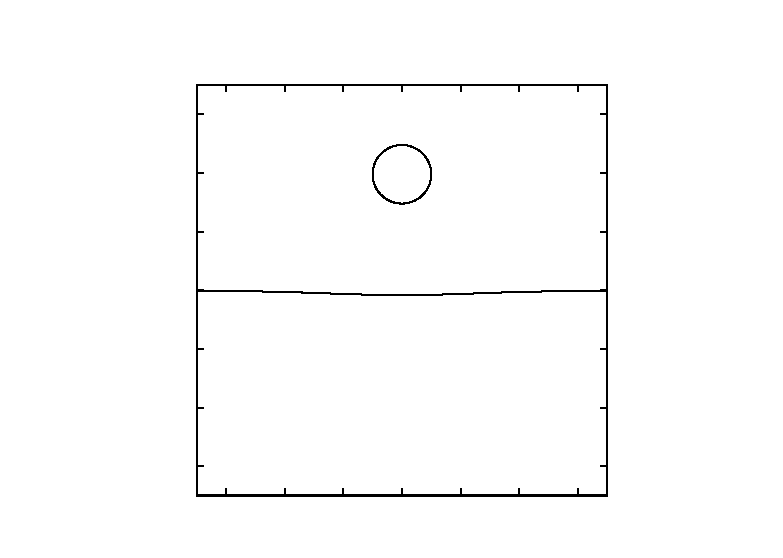
\includegraphics{floating_frame2}}%
    \gplfronttext
  \end{picture}%
\endgroup
}
        \caption{}
        \label{fig:floating_frame2}
      \end{subfigure}
      ~
      \begin{subfigure}[b]{0.45\textwidth}
        \resizebox{\textwidth}{!}{\Large % GNUPLOT: LaTeX picture with Postscript
\begingroup
  \makeatletter
  \providecommand\color[2][]{%
    \GenericError{(gnuplot) \space\space\space\@spaces}{%
      Package color not loaded in conjunction with
      terminal option `colourtext'%
    }{See the gnuplot documentation for explanation.%
    }{Either use 'blacktext' in gnuplot or load the package
      color.sty in LaTeX.}%
    \renewcommand\color[2][]{}%
  }%
  \providecommand\includegraphics[2][]{%
    \GenericError{(gnuplot) \space\space\space\@spaces}{%
      Package graphicx or graphics not loaded%
    }{See the gnuplot documentation for explanation.%
    }{The gnuplot epslatex terminal needs graphicx.sty or graphics.sty.}%
    \renewcommand\includegraphics[2][]{}%
  }%
  \providecommand\rotatebox[2]{#2}%
  \@ifundefined{ifGPcolor}{%
    \newif\ifGPcolor
    \GPcolorfalse
  }{}%
  \@ifundefined{ifGPblacktext}{%
    \newif\ifGPblacktext
    \GPblacktexttrue
  }{}%
  % define a \g@addto@macro without @ in the name:
  \let\gplgaddtomacro\g@addto@macro
  % define empty templates for all commands taking text:
  \gdef\gplbacktext{}%
  \gdef\gplfronttext{}%
  \makeatother
  \ifGPblacktext
    % no textcolor at all
    \def\colorrgb#1{}%
    \def\colorgray#1{}%
  \else
    % gray or color?
    \ifGPcolor
      \def\colorrgb#1{\color[rgb]{#1}}%
      \def\colorgray#1{\color[gray]{#1}}%
      \expandafter\def\csname LTw\endcsname{\color{white}}%
      \expandafter\def\csname LTb\endcsname{\color{black}}%
      \expandafter\def\csname LTa\endcsname{\color{black}}%
      \expandafter\def\csname LT0\endcsname{\color[rgb]{1,0,0}}%
      \expandafter\def\csname LT1\endcsname{\color[rgb]{0,1,0}}%
      \expandafter\def\csname LT2\endcsname{\color[rgb]{0,0,1}}%
      \expandafter\def\csname LT3\endcsname{\color[rgb]{1,0,1}}%
      \expandafter\def\csname LT4\endcsname{\color[rgb]{0,1,1}}%
      \expandafter\def\csname LT5\endcsname{\color[rgb]{1,1,0}}%
      \expandafter\def\csname LT6\endcsname{\color[rgb]{0,0,0}}%
      \expandafter\def\csname LT7\endcsname{\color[rgb]{1,0.3,0}}%
      \expandafter\def\csname LT8\endcsname{\color[rgb]{0.5,0.5,0.5}}%
    \else
      % gray
      \def\colorrgb#1{\color{black}}%
      \def\colorgray#1{\color[gray]{#1}}%
      \expandafter\def\csname LTw\endcsname{\color{white}}%
      \expandafter\def\csname LTb\endcsname{\color{black}}%
      \expandafter\def\csname LTa\endcsname{\color{black}}%
      \expandafter\def\csname LT0\endcsname{\color{black}}%
      \expandafter\def\csname LT1\endcsname{\color{black}}%
      \expandafter\def\csname LT2\endcsname{\color{black}}%
      \expandafter\def\csname LT3\endcsname{\color{black}}%
      \expandafter\def\csname LT4\endcsname{\color{black}}%
      \expandafter\def\csname LT5\endcsname{\color{black}}%
      \expandafter\def\csname LT6\endcsname{\color{black}}%
      \expandafter\def\csname LT7\endcsname{\color{black}}%
      \expandafter\def\csname LT8\endcsname{\color{black}}%
    \fi
  \fi
    \setlength{\unitlength}{0.0500bp}%
    \ifx\gptboxheight\undefined%
      \newlength{\gptboxheight}%
      \newlength{\gptboxwidth}%
      \newsavebox{\gptboxtext}%
    \fi%
    \setlength{\fboxrule}{0.5pt}%
    \setlength{\fboxsep}{1pt}%
\begin{picture}(7200.00,5040.00)%
    \gplgaddtomacro\gplbacktext{%
      \csname LTb\endcsname%
      \put(1597,721){\makebox(0,0)[r]{\strut{}$-6$}}%
      \put(1597,1284){\makebox(0,0)[r]{\strut{}$-4$}}%
      \put(1597,1847){\makebox(0,0)[r]{\strut{}$-2$}}%
      \put(1597,2410){\makebox(0,0)[r]{\strut{}$0$}}%
      \put(1597,2972){\makebox(0,0)[r]{\strut{}$2$}}%
      \put(1597,3535){\makebox(0,0)[r]{\strut{}$4$}}%
      \put(1597,4098){\makebox(0,0)[r]{\strut{}$6$}}%
      \put(2010,220){\makebox(0,0){\strut{}$-6$}}%
      \put(2573,220){\makebox(0,0){\strut{}$-4$}}%
      \put(3136,220){\makebox(0,0){\strut{}$-2$}}%
      \put(3699,220){\makebox(0,0){\strut{}$0$}}%
      \put(4261,220){\makebox(0,0){\strut{}$2$}}%
      \put(4824,220){\makebox(0,0){\strut{}$4$}}%
      \put(5387,220){\makebox(0,0){\strut{}$6$}}%
    }%
    \gplgaddtomacro\gplfronttext{%
      \csname LTb\endcsname%
      \put(3698,4709){\makebox(0,0){\strut{}t = 9.37}}%
    }%
    \gplbacktext
    \put(0,0){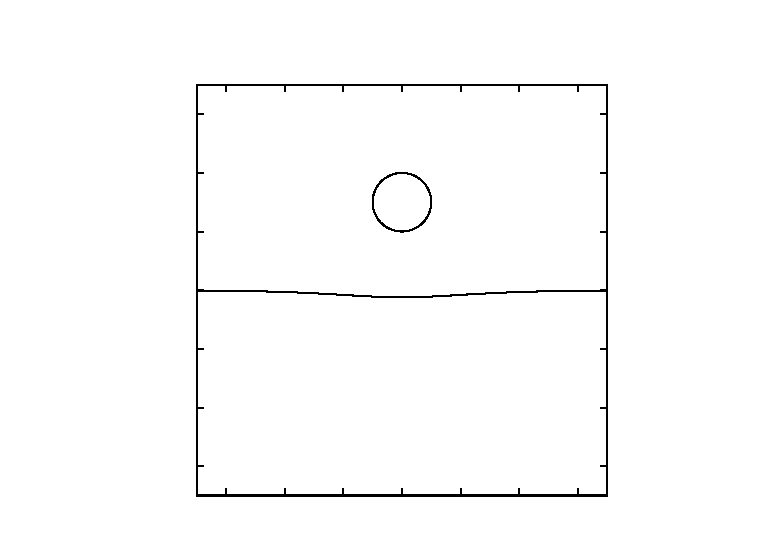
\includegraphics{../../Programming/sinking_bim_write_up/trunk/floating_frame3}}%
    \gplfronttext
  \end{picture}%
\endgroup
}
        \caption{}
        \label{fig:floating_frame3}
      \end{subfigure}
      
      \begin{subfigure}[b]{0.45\textwidth}
        \resizebox{\textwidth}{!}{\Large % GNUPLOT: LaTeX picture with Postscript
\begingroup
  \makeatletter
  \providecommand\color[2][]{%
    \GenericError{(gnuplot) \space\space\space\@spaces}{%
      Package color not loaded in conjunction with
      terminal option `colourtext'%
    }{See the gnuplot documentation for explanation.%
    }{Either use 'blacktext' in gnuplot or load the package
      color.sty in LaTeX.}%
    \renewcommand\color[2][]{}%
  }%
  \providecommand\includegraphics[2][]{%
    \GenericError{(gnuplot) \space\space\space\@spaces}{%
      Package graphicx or graphics not loaded%
    }{See the gnuplot documentation for explanation.%
    }{The gnuplot epslatex terminal needs graphicx.sty or graphics.sty.}%
    \renewcommand\includegraphics[2][]{}%
  }%
  \providecommand\rotatebox[2]{#2}%
  \@ifundefined{ifGPcolor}{%
    \newif\ifGPcolor
    \GPcolorfalse
  }{}%
  \@ifundefined{ifGPblacktext}{%
    \newif\ifGPblacktext
    \GPblacktexttrue
  }{}%
  % define a \g@addto@macro without @ in the name:
  \let\gplgaddtomacro\g@addto@macro
  % define empty templates for all commands taking text:
  \gdef\gplbacktext{}%
  \gdef\gplfronttext{}%
  \makeatother
  \ifGPblacktext
    % no textcolor at all
    \def\colorrgb#1{}%
    \def\colorgray#1{}%
  \else
    % gray or color?
    \ifGPcolor
      \def\colorrgb#1{\color[rgb]{#1}}%
      \def\colorgray#1{\color[gray]{#1}}%
      \expandafter\def\csname LTw\endcsname{\color{white}}%
      \expandafter\def\csname LTb\endcsname{\color{black}}%
      \expandafter\def\csname LTa\endcsname{\color{black}}%
      \expandafter\def\csname LT0\endcsname{\color[rgb]{1,0,0}}%
      \expandafter\def\csname LT1\endcsname{\color[rgb]{0,1,0}}%
      \expandafter\def\csname LT2\endcsname{\color[rgb]{0,0,1}}%
      \expandafter\def\csname LT3\endcsname{\color[rgb]{1,0,1}}%
      \expandafter\def\csname LT4\endcsname{\color[rgb]{0,1,1}}%
      \expandafter\def\csname LT5\endcsname{\color[rgb]{1,1,0}}%
      \expandafter\def\csname LT6\endcsname{\color[rgb]{0,0,0}}%
      \expandafter\def\csname LT7\endcsname{\color[rgb]{1,0.3,0}}%
      \expandafter\def\csname LT8\endcsname{\color[rgb]{0.5,0.5,0.5}}%
    \else
      % gray
      \def\colorrgb#1{\color{black}}%
      \def\colorgray#1{\color[gray]{#1}}%
      \expandafter\def\csname LTw\endcsname{\color{white}}%
      \expandafter\def\csname LTb\endcsname{\color{black}}%
      \expandafter\def\csname LTa\endcsname{\color{black}}%
      \expandafter\def\csname LT0\endcsname{\color{black}}%
      \expandafter\def\csname LT1\endcsname{\color{black}}%
      \expandafter\def\csname LT2\endcsname{\color{black}}%
      \expandafter\def\csname LT3\endcsname{\color{black}}%
      \expandafter\def\csname LT4\endcsname{\color{black}}%
      \expandafter\def\csname LT5\endcsname{\color{black}}%
      \expandafter\def\csname LT6\endcsname{\color{black}}%
      \expandafter\def\csname LT7\endcsname{\color{black}}%
      \expandafter\def\csname LT8\endcsname{\color{black}}%
    \fi
  \fi
    \setlength{\unitlength}{0.0500bp}%
    \ifx\gptboxheight\undefined%
      \newlength{\gptboxheight}%
      \newlength{\gptboxwidth}%
      \newsavebox{\gptboxtext}%
    \fi%
    \setlength{\fboxrule}{0.5pt}%
    \setlength{\fboxsep}{1pt}%
\begin{picture}(7200.00,5040.00)%
    \gplgaddtomacro\gplbacktext{%
      \csname LTb\endcsname%
      \put(1597,721){\makebox(0,0)[r]{\strut{}$-6$}}%
      \put(1597,1284){\makebox(0,0)[r]{\strut{}$-4$}}%
      \put(1597,1847){\makebox(0,0)[r]{\strut{}$-2$}}%
      \put(1597,2410){\makebox(0,0)[r]{\strut{}$0$}}%
      \put(1597,2972){\makebox(0,0)[r]{\strut{}$2$}}%
      \put(1597,3535){\makebox(0,0)[r]{\strut{}$4$}}%
      \put(1597,4098){\makebox(0,0)[r]{\strut{}$6$}}%
      \put(2010,220){\makebox(0,0){\strut{}$-6$}}%
      \put(2573,220){\makebox(0,0){\strut{}$-4$}}%
      \put(3136,220){\makebox(0,0){\strut{}$-2$}}%
      \put(3699,220){\makebox(0,0){\strut{}$0$}}%
      \put(4261,220){\makebox(0,0){\strut{}$2$}}%
      \put(4824,220){\makebox(0,0){\strut{}$4$}}%
      \put(5387,220){\makebox(0,0){\strut{}$6$}}%
    }%
    \gplgaddtomacro\gplfronttext{%
      \csname LTb\endcsname%
      \put(3698,4709){\makebox(0,0){\strut{}t = 10.76}}%
    }%
    \gplbacktext
    \put(0,0){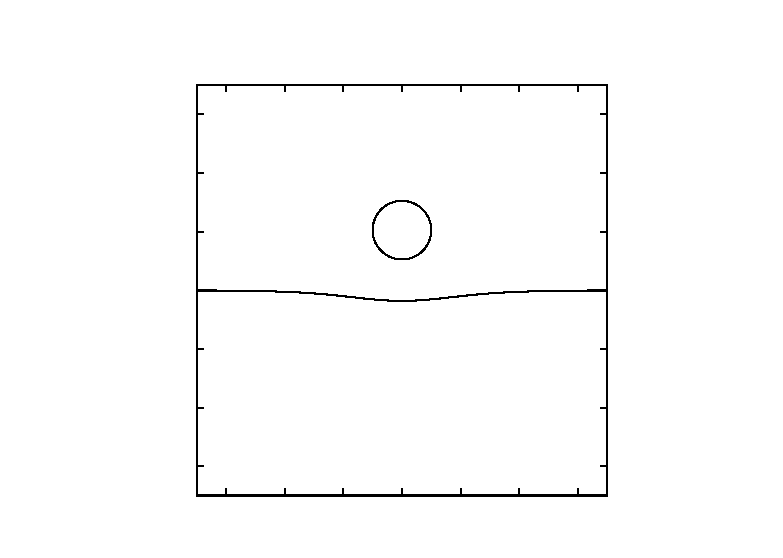
\includegraphics{../../Programming/sinking_bim_write_up/trunk/floating_frame4}}%
    \gplfronttext
  \end{picture}%
\endgroup
}
        \caption{}
        \label{fig:floating_frame4}
      \end{subfigure}
      ~
      \begin{subfigure}[b]{0.45\textwidth}
        \resizebox{\textwidth}{!}{\Large % GNUPLOT: LaTeX picture with Postscript
\begingroup
  \makeatletter
  \providecommand\color[2][]{%
    \GenericError{(gnuplot) \space\space\space\@spaces}{%
      Package color not loaded in conjunction with
      terminal option `colourtext'%
    }{See the gnuplot documentation for explanation.%
    }{Either use 'blacktext' in gnuplot or load the package
      color.sty in LaTeX.}%
    \renewcommand\color[2][]{}%
  }%
  \providecommand\includegraphics[2][]{%
    \GenericError{(gnuplot) \space\space\space\@spaces}{%
      Package graphicx or graphics not loaded%
    }{See the gnuplot documentation for explanation.%
    }{The gnuplot epslatex terminal needs graphicx.sty or graphics.sty.}%
    \renewcommand\includegraphics[2][]{}%
  }%
  \providecommand\rotatebox[2]{#2}%
  \@ifundefined{ifGPcolor}{%
    \newif\ifGPcolor
    \GPcolorfalse
  }{}%
  \@ifundefined{ifGPblacktext}{%
    \newif\ifGPblacktext
    \GPblacktexttrue
  }{}%
  % define a \g@addto@macro without @ in the name:
  \let\gplgaddtomacro\g@addto@macro
  % define empty templates for all commands taking text:
  \gdef\gplbacktext{}%
  \gdef\gplfronttext{}%
  \makeatother
  \ifGPblacktext
    % no textcolor at all
    \def\colorrgb#1{}%
    \def\colorgray#1{}%
  \else
    % gray or color?
    \ifGPcolor
      \def\colorrgb#1{\color[rgb]{#1}}%
      \def\colorgray#1{\color[gray]{#1}}%
      \expandafter\def\csname LTw\endcsname{\color{white}}%
      \expandafter\def\csname LTb\endcsname{\color{black}}%
      \expandafter\def\csname LTa\endcsname{\color{black}}%
      \expandafter\def\csname LT0\endcsname{\color[rgb]{1,0,0}}%
      \expandafter\def\csname LT1\endcsname{\color[rgb]{0,1,0}}%
      \expandafter\def\csname LT2\endcsname{\color[rgb]{0,0,1}}%
      \expandafter\def\csname LT3\endcsname{\color[rgb]{1,0,1}}%
      \expandafter\def\csname LT4\endcsname{\color[rgb]{0,1,1}}%
      \expandafter\def\csname LT5\endcsname{\color[rgb]{1,1,0}}%
      \expandafter\def\csname LT6\endcsname{\color[rgb]{0,0,0}}%
      \expandafter\def\csname LT7\endcsname{\color[rgb]{1,0.3,0}}%
      \expandafter\def\csname LT8\endcsname{\color[rgb]{0.5,0.5,0.5}}%
    \else
      % gray
      \def\colorrgb#1{\color{black}}%
      \def\colorgray#1{\color[gray]{#1}}%
      \expandafter\def\csname LTw\endcsname{\color{white}}%
      \expandafter\def\csname LTb\endcsname{\color{black}}%
      \expandafter\def\csname LTa\endcsname{\color{black}}%
      \expandafter\def\csname LT0\endcsname{\color{black}}%
      \expandafter\def\csname LT1\endcsname{\color{black}}%
      \expandafter\def\csname LT2\endcsname{\color{black}}%
      \expandafter\def\csname LT3\endcsname{\color{black}}%
      \expandafter\def\csname LT4\endcsname{\color{black}}%
      \expandafter\def\csname LT5\endcsname{\color{black}}%
      \expandafter\def\csname LT6\endcsname{\color{black}}%
      \expandafter\def\csname LT7\endcsname{\color{black}}%
      \expandafter\def\csname LT8\endcsname{\color{black}}%
    \fi
  \fi
    \setlength{\unitlength}{0.0500bp}%
    \ifx\gptboxheight\undefined%
      \newlength{\gptboxheight}%
      \newlength{\gptboxwidth}%
      \newsavebox{\gptboxtext}%
    \fi%
    \setlength{\fboxrule}{0.5pt}%
    \setlength{\fboxsep}{1pt}%
\begin{picture}(7200.00,5040.00)%
    \gplgaddtomacro\gplbacktext{%
      \csname LTb\endcsname%
      \put(1597,721){\makebox(0,0)[r]{\strut{}$-6$}}%
      \put(1597,1284){\makebox(0,0)[r]{\strut{}$-4$}}%
      \put(1597,1847){\makebox(0,0)[r]{\strut{}$-2$}}%
      \put(1597,2410){\makebox(0,0)[r]{\strut{}$0$}}%
      \put(1597,2972){\makebox(0,0)[r]{\strut{}$2$}}%
      \put(1597,3535){\makebox(0,0)[r]{\strut{}$4$}}%
      \put(1597,4098){\makebox(0,0)[r]{\strut{}$6$}}%
      \put(2010,220){\makebox(0,0){\strut{}$-6$}}%
      \put(2573,220){\makebox(0,0){\strut{}$-4$}}%
      \put(3136,220){\makebox(0,0){\strut{}$-2$}}%
      \put(3699,220){\makebox(0,0){\strut{}$0$}}%
      \put(4261,220){\makebox(0,0){\strut{}$2$}}%
      \put(4824,220){\makebox(0,0){\strut{}$4$}}%
      \put(5387,220){\makebox(0,0){\strut{}$6$}}%
    }%
    \gplgaddtomacro\gplfronttext{%
      \csname LTb\endcsname%
      \put(3698,4709){\makebox(0,0){\strut{}t = 12.69}}%
    }%
    \gplbacktext
    \put(0,0){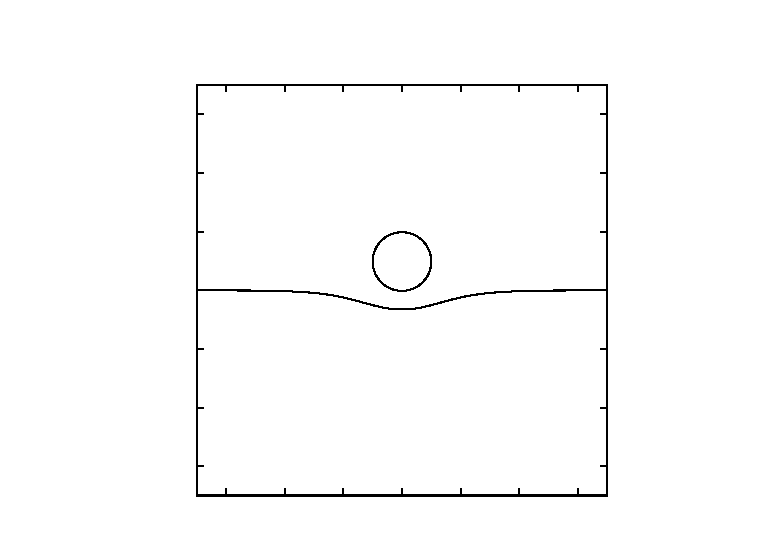
\includegraphics{floating_frame5}}%
    \gplfronttext
  \end{picture}%
\endgroup
}
        \caption{}
        \label{fig:floating_frame5}
      \end{subfigure}
      
      \begin{subfigure}[b]{0.45\textwidth}
        \resizebox{\textwidth}{!}{\Large % GNUPLOT: LaTeX picture with Postscript
\begingroup
  \makeatletter
  \providecommand\color[2][]{%
    \GenericError{(gnuplot) \space\space\space\@spaces}{%
      Package color not loaded in conjunction with
      terminal option `colourtext'%
    }{See the gnuplot documentation for explanation.%
    }{Either use 'blacktext' in gnuplot or load the package
      color.sty in LaTeX.}%
    \renewcommand\color[2][]{}%
  }%
  \providecommand\includegraphics[2][]{%
    \GenericError{(gnuplot) \space\space\space\@spaces}{%
      Package graphicx or graphics not loaded%
    }{See the gnuplot documentation for explanation.%
    }{The gnuplot epslatex terminal needs graphicx.sty or graphics.sty.}%
    \renewcommand\includegraphics[2][]{}%
  }%
  \providecommand\rotatebox[2]{#2}%
  \@ifundefined{ifGPcolor}{%
    \newif\ifGPcolor
    \GPcolorfalse
  }{}%
  \@ifundefined{ifGPblacktext}{%
    \newif\ifGPblacktext
    \GPblacktexttrue
  }{}%
  % define a \g@addto@macro without @ in the name:
  \let\gplgaddtomacro\g@addto@macro
  % define empty templates for all commands taking text:
  \gdef\gplbacktext{}%
  \gdef\gplfronttext{}%
  \makeatother
  \ifGPblacktext
    % no textcolor at all
    \def\colorrgb#1{}%
    \def\colorgray#1{}%
  \else
    % gray or color?
    \ifGPcolor
      \def\colorrgb#1{\color[rgb]{#1}}%
      \def\colorgray#1{\color[gray]{#1}}%
      \expandafter\def\csname LTw\endcsname{\color{white}}%
      \expandafter\def\csname LTb\endcsname{\color{black}}%
      \expandafter\def\csname LTa\endcsname{\color{black}}%
      \expandafter\def\csname LT0\endcsname{\color[rgb]{1,0,0}}%
      \expandafter\def\csname LT1\endcsname{\color[rgb]{0,1,0}}%
      \expandafter\def\csname LT2\endcsname{\color[rgb]{0,0,1}}%
      \expandafter\def\csname LT3\endcsname{\color[rgb]{1,0,1}}%
      \expandafter\def\csname LT4\endcsname{\color[rgb]{0,1,1}}%
      \expandafter\def\csname LT5\endcsname{\color[rgb]{1,1,0}}%
      \expandafter\def\csname LT6\endcsname{\color[rgb]{0,0,0}}%
      \expandafter\def\csname LT7\endcsname{\color[rgb]{1,0.3,0}}%
      \expandafter\def\csname LT8\endcsname{\color[rgb]{0.5,0.5,0.5}}%
    \else
      % gray
      \def\colorrgb#1{\color{black}}%
      \def\colorgray#1{\color[gray]{#1}}%
      \expandafter\def\csname LTw\endcsname{\color{white}}%
      \expandafter\def\csname LTb\endcsname{\color{black}}%
      \expandafter\def\csname LTa\endcsname{\color{black}}%
      \expandafter\def\csname LT0\endcsname{\color{black}}%
      \expandafter\def\csname LT1\endcsname{\color{black}}%
      \expandafter\def\csname LT2\endcsname{\color{black}}%
      \expandafter\def\csname LT3\endcsname{\color{black}}%
      \expandafter\def\csname LT4\endcsname{\color{black}}%
      \expandafter\def\csname LT5\endcsname{\color{black}}%
      \expandafter\def\csname LT6\endcsname{\color{black}}%
      \expandafter\def\csname LT7\endcsname{\color{black}}%
      \expandafter\def\csname LT8\endcsname{\color{black}}%
    \fi
  \fi
    \setlength{\unitlength}{0.0500bp}%
    \ifx\gptboxheight\undefined%
      \newlength{\gptboxheight}%
      \newlength{\gptboxwidth}%
      \newsavebox{\gptboxtext}%
    \fi%
    \setlength{\fboxrule}{0.5pt}%
    \setlength{\fboxsep}{1pt}%
\begin{picture}(7200.00,5040.00)%
    \gplgaddtomacro\gplbacktext{%
      \csname LTb\endcsname%
      \put(1597,721){\makebox(0,0)[r]{\strut{}$-6$}}%
      \put(1597,1284){\makebox(0,0)[r]{\strut{}$-4$}}%
      \put(1597,1847){\makebox(0,0)[r]{\strut{}$-2$}}%
      \put(1597,2410){\makebox(0,0)[r]{\strut{}$0$}}%
      \put(1597,2972){\makebox(0,0)[r]{\strut{}$2$}}%
      \put(1597,3535){\makebox(0,0)[r]{\strut{}$4$}}%
      \put(1597,4098){\makebox(0,0)[r]{\strut{}$6$}}%
      \put(2010,220){\makebox(0,0){\strut{}$-6$}}%
      \put(2573,220){\makebox(0,0){\strut{}$-4$}}%
      \put(3136,220){\makebox(0,0){\strut{}$-2$}}%
      \put(3699,220){\makebox(0,0){\strut{}$0$}}%
      \put(4261,220){\makebox(0,0){\strut{}$2$}}%
      \put(4824,220){\makebox(0,0){\strut{}$4$}}%
      \put(5387,220){\makebox(0,0){\strut{}$6$}}%
    }%
    \gplgaddtomacro\gplfronttext{%
      \csname LTb\endcsname%
      \put(3698,4709){\makebox(0,0){\strut{}t = 15.74}}%
    }%
    \gplbacktext
    \put(0,0){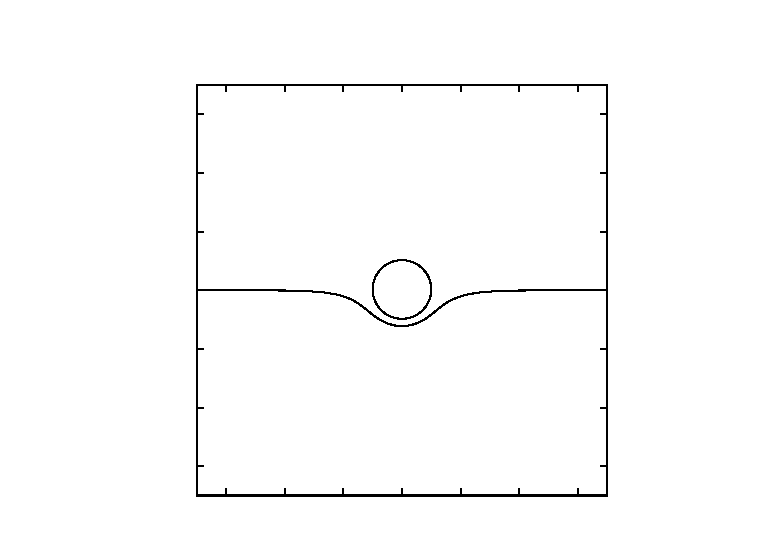
\includegraphics{floating_frame6}}%
    \gplfronttext
  \end{picture}%
\endgroup
}
        \caption{}
        \label{fig:floating_frame6}
      \end{subfigure}
      ~
      \begin{subfigure}[b]{0.45\textwidth}
        \resizebox{\textwidth}{!}{\Large % GNUPLOT: LaTeX picture with Postscript
\begingroup
  \makeatletter
  \providecommand\color[2][]{%
    \GenericError{(gnuplot) \space\space\space\@spaces}{%
      Package color not loaded in conjunction with
      terminal option `colourtext'%
    }{See the gnuplot documentation for explanation.%
    }{Either use 'blacktext' in gnuplot or load the package
      color.sty in LaTeX.}%
    \renewcommand\color[2][]{}%
  }%
  \providecommand\includegraphics[2][]{%
    \GenericError{(gnuplot) \space\space\space\@spaces}{%
      Package graphicx or graphics not loaded%
    }{See the gnuplot documentation for explanation.%
    }{The gnuplot epslatex terminal needs graphicx.sty or graphics.sty.}%
    \renewcommand\includegraphics[2][]{}%
  }%
  \providecommand\rotatebox[2]{#2}%
  \@ifundefined{ifGPcolor}{%
    \newif\ifGPcolor
    \GPcolorfalse
  }{}%
  \@ifundefined{ifGPblacktext}{%
    \newif\ifGPblacktext
    \GPblacktexttrue
  }{}%
  % define a \g@addto@macro without @ in the name:
  \let\gplgaddtomacro\g@addto@macro
  % define empty templates for all commands taking text:
  \gdef\gplbacktext{}%
  \gdef\gplfronttext{}%
  \makeatother
  \ifGPblacktext
    % no textcolor at all
    \def\colorrgb#1{}%
    \def\colorgray#1{}%
  \else
    % gray or color?
    \ifGPcolor
      \def\colorrgb#1{\color[rgb]{#1}}%
      \def\colorgray#1{\color[gray]{#1}}%
      \expandafter\def\csname LTw\endcsname{\color{white}}%
      \expandafter\def\csname LTb\endcsname{\color{black}}%
      \expandafter\def\csname LTa\endcsname{\color{black}}%
      \expandafter\def\csname LT0\endcsname{\color[rgb]{1,0,0}}%
      \expandafter\def\csname LT1\endcsname{\color[rgb]{0,1,0}}%
      \expandafter\def\csname LT2\endcsname{\color[rgb]{0,0,1}}%
      \expandafter\def\csname LT3\endcsname{\color[rgb]{1,0,1}}%
      \expandafter\def\csname LT4\endcsname{\color[rgb]{0,1,1}}%
      \expandafter\def\csname LT5\endcsname{\color[rgb]{1,1,0}}%
      \expandafter\def\csname LT6\endcsname{\color[rgb]{0,0,0}}%
      \expandafter\def\csname LT7\endcsname{\color[rgb]{1,0.3,0}}%
      \expandafter\def\csname LT8\endcsname{\color[rgb]{0.5,0.5,0.5}}%
    \else
      % gray
      \def\colorrgb#1{\color{black}}%
      \def\colorgray#1{\color[gray]{#1}}%
      \expandafter\def\csname LTw\endcsname{\color{white}}%
      \expandafter\def\csname LTb\endcsname{\color{black}}%
      \expandafter\def\csname LTa\endcsname{\color{black}}%
      \expandafter\def\csname LT0\endcsname{\color{black}}%
      \expandafter\def\csname LT1\endcsname{\color{black}}%
      \expandafter\def\csname LT2\endcsname{\color{black}}%
      \expandafter\def\csname LT3\endcsname{\color{black}}%
      \expandafter\def\csname LT4\endcsname{\color{black}}%
      \expandafter\def\csname LT5\endcsname{\color{black}}%
      \expandafter\def\csname LT6\endcsname{\color{black}}%
      \expandafter\def\csname LT7\endcsname{\color{black}}%
      \expandafter\def\csname LT8\endcsname{\color{black}}%
    \fi
  \fi
    \setlength{\unitlength}{0.0500bp}%
    \ifx\gptboxheight\undefined%
      \newlength{\gptboxheight}%
      \newlength{\gptboxwidth}%
      \newsavebox{\gptboxtext}%
    \fi%
    \setlength{\fboxrule}{0.5pt}%
    \setlength{\fboxsep}{1pt}%
\begin{picture}(7200.00,5040.00)%
    \gplgaddtomacro\gplbacktext{%
      \csname LTb\endcsname%
      \put(1597,721){\makebox(0,0)[r]{\strut{}$-6$}}%
      \put(1597,1284){\makebox(0,0)[r]{\strut{}$-4$}}%
      \put(1597,1847){\makebox(0,0)[r]{\strut{}$-2$}}%
      \put(1597,2410){\makebox(0,0)[r]{\strut{}$0$}}%
      \put(1597,2972){\makebox(0,0)[r]{\strut{}$2$}}%
      \put(1597,3535){\makebox(0,0)[r]{\strut{}$4$}}%
      \put(1597,4098){\makebox(0,0)[r]{\strut{}$6$}}%
      \put(2010,220){\makebox(0,0){\strut{}$-6$}}%
      \put(2573,220){\makebox(0,0){\strut{}$-4$}}%
      \put(3136,220){\makebox(0,0){\strut{}$-2$}}%
      \put(3699,220){\makebox(0,0){\strut{}$0$}}%
      \put(4261,220){\makebox(0,0){\strut{}$2$}}%
      \put(4824,220){\makebox(0,0){\strut{}$4$}}%
      \put(5387,220){\makebox(0,0){\strut{}$6$}}%
    }%
    \gplgaddtomacro\gplfronttext{%
      \csname LTb\endcsname%
      \put(3698,4709){\makebox(0,0){\strut{}t = 999.99}}%
    }%
    \gplbacktext
    \put(0,0){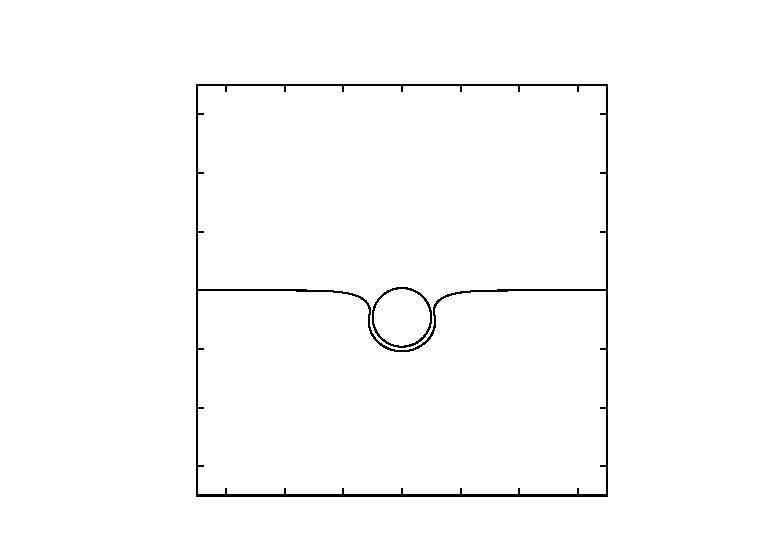
\includegraphics{../../Programming/sinking_bim_write_up/trunk/floating_frame7}}%
    \gplfronttext
  \end{picture}%
\endgroup
}
        \caption{}
        \label{fig:floating_frame7}
      \end{subfigure}
      \caption{Settling of a sphere onto the interface when $D = 2.2$, $\Bo = 2.5$ and $\lambda = 1$. The interface deforms as the sphere approaches and the sphere attains an equilibrium position with a thin film of fluid trapped between the sphere and the interface.}\label{fig:floating_frame}
    \end{figure}

  \begin{figure}
    \resizebox{0.9\textwidth}{!}{\large % GNUPLOT: LaTeX picture with Postscript
\begingroup
  \makeatletter
  \providecommand\color[2][]{%
    \GenericError{(gnuplot) \space\space\space\@spaces}{%
      Package color not loaded in conjunction with
      terminal option `colourtext'%
    }{See the gnuplot documentation for explanation.%
    }{Either use 'blacktext' in gnuplot or load the package
      color.sty in LaTeX.}%
    \renewcommand\color[2][]{}%
  }%
  \providecommand\includegraphics[2][]{%
    \GenericError{(gnuplot) \space\space\space\@spaces}{%
      Package graphicx or graphics not loaded%
    }{See the gnuplot documentation for explanation.%
    }{The gnuplot epslatex terminal needs graphicx.sty or graphics.sty.}%
    \renewcommand\includegraphics[2][]{}%
  }%
  \providecommand\rotatebox[2]{#2}%
  \@ifundefined{ifGPcolor}{%
    \newif\ifGPcolor
    \GPcolorfalse
  }{}%
  \@ifundefined{ifGPblacktext}{%
    \newif\ifGPblacktext
    \GPblacktexttrue
  }{}%
  % define a \g@addto@macro without @ in the name:
  \let\gplgaddtomacro\g@addto@macro
  % define empty templates for all commands taking text:
  \gdef\gplbacktext{}%
  \gdef\gplfronttext{}%
  \makeatother
  \ifGPblacktext
    % no textcolor at all
    \def\colorrgb#1{}%
    \def\colorgray#1{}%
  \else
    % gray or color?
    \ifGPcolor
      \def\colorrgb#1{\color[rgb]{#1}}%
      \def\colorgray#1{\color[gray]{#1}}%
      \expandafter\def\csname LTw\endcsname{\color{white}}%
      \expandafter\def\csname LTb\endcsname{\color{black}}%
      \expandafter\def\csname LTa\endcsname{\color{black}}%
      \expandafter\def\csname LT0\endcsname{\color[rgb]{1,0,0}}%
      \expandafter\def\csname LT1\endcsname{\color[rgb]{0,1,0}}%
      \expandafter\def\csname LT2\endcsname{\color[rgb]{0,0,1}}%
      \expandafter\def\csname LT3\endcsname{\color[rgb]{1,0,1}}%
      \expandafter\def\csname LT4\endcsname{\color[rgb]{0,1,1}}%
      \expandafter\def\csname LT5\endcsname{\color[rgb]{1,1,0}}%
      \expandafter\def\csname LT6\endcsname{\color[rgb]{0,0,0}}%
      \expandafter\def\csname LT7\endcsname{\color[rgb]{1,0.3,0}}%
      \expandafter\def\csname LT8\endcsname{\color[rgb]{0.5,0.5,0.5}}%
    \else
      % gray
      \def\colorrgb#1{\color{black}}%
      \def\colorgray#1{\color[gray]{#1}}%
      \expandafter\def\csname LTw\endcsname{\color{white}}%
      \expandafter\def\csname LTb\endcsname{\color{black}}%
      \expandafter\def\csname LTa\endcsname{\color{black}}%
      \expandafter\def\csname LT0\endcsname{\color{black}}%
      \expandafter\def\csname LT1\endcsname{\color{black}}%
      \expandafter\def\csname LT2\endcsname{\color{black}}%
      \expandafter\def\csname LT3\endcsname{\color{black}}%
      \expandafter\def\csname LT4\endcsname{\color{black}}%
      \expandafter\def\csname LT5\endcsname{\color{black}}%
      \expandafter\def\csname LT6\endcsname{\color{black}}%
      \expandafter\def\csname LT7\endcsname{\color{black}}%
      \expandafter\def\csname LT8\endcsname{\color{black}}%
    \fi
  \fi
    \setlength{\unitlength}{0.0500bp}%
    \ifx\gptboxheight\undefined%
      \newlength{\gptboxheight}%
      \newlength{\gptboxwidth}%
      \newsavebox{\gptboxtext}%
    \fi%
    \setlength{\fboxrule}{0.5pt}%
    \setlength{\fboxsep}{1pt}%
\begin{picture}(7200.00,5040.00)%
    \gplgaddtomacro\gplbacktext{%
      \csname LTb\endcsname%
      \put(682,704){\makebox(0,0)[r]{\strut{}$-2$}}%
      \put(682,1286){\makebox(0,0)[r]{\strut{}$0$}}%
      \put(682,1867){\makebox(0,0)[r]{\strut{}$2$}}%
      \put(682,2449){\makebox(0,0)[r]{\strut{}$4$}}%
      \put(682,3030){\makebox(0,0)[r]{\strut{}$6$}}%
      \put(682,3612){\makebox(0,0)[r]{\strut{}$8$}}%
      \put(682,4193){\makebox(0,0)[r]{\strut{}$10$}}%
      \put(682,4775){\makebox(0,0)[r]{\strut{}$12$}}%
      \put(814,484){\makebox(0,0){\strut{}$0$}}%
      \put(2012,484){\makebox(0,0){\strut{}$100$}}%
      \put(3210,484){\makebox(0,0){\strut{}$200$}}%
      \put(4407,484){\makebox(0,0){\strut{}$300$}}%
      \put(5605,484){\makebox(0,0){\strut{}$400$}}%
      \put(6803,484){\makebox(0,0){\strut{}$500$}}%
    }%
    \gplgaddtomacro\gplfronttext{%
      \csname LTb\endcsname%
      \put(176,2739){\rotatebox{-270}{\makebox(0,0){\strut{}$z_{\text{s}}$}}}%
      \put(3808,154){\makebox(0,0){\strut{}$t$}}%
    }%
    \gplbacktext
    \put(0,0){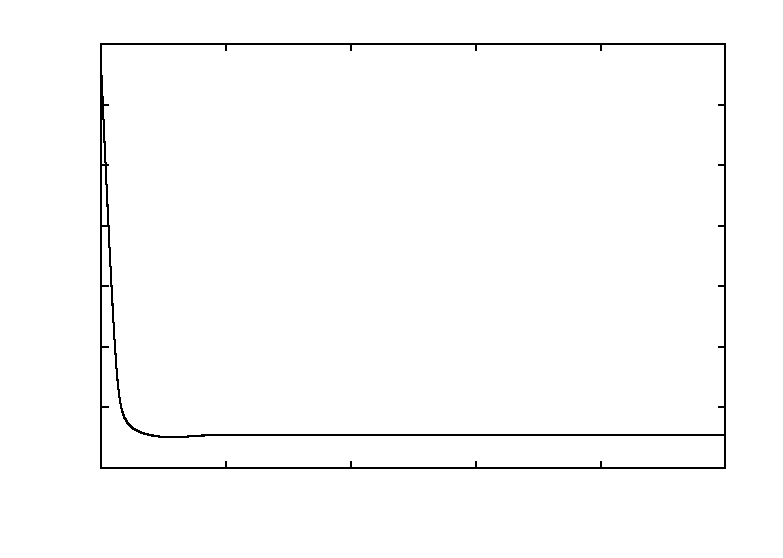
\includegraphics{floating_traj}}%
    \gplfronttext
  \end{picture}%
\endgroup
}
    \caption{Position curve of the sphere, which is seen to attain an equilibrium position at the interface. \label{fig:floating_traj}}
  \end{figure}


    \begin{figure}
      \centering
      \begin{subfigure}[b]{0.45\textwidth}
        \resizebox{\textwidth}{!}{\Large % GNUPLOT: LaTeX picture with Postscript
\begingroup
  \makeatletter
  \providecommand\color[2][]{%
    \GenericError{(gnuplot) \space\space\space\@spaces}{%
      Package color not loaded in conjunction with
      terminal option `colourtext'%
    }{See the gnuplot documentation for explanation.%
    }{Either use 'blacktext' in gnuplot or load the package
      color.sty in LaTeX.}%
    \renewcommand\color[2][]{}%
  }%
  \providecommand\includegraphics[2][]{%
    \GenericError{(gnuplot) \space\space\space\@spaces}{%
      Package graphicx or graphics not loaded%
    }{See the gnuplot documentation for explanation.%
    }{The gnuplot epslatex terminal needs graphicx.sty or graphics.sty.}%
    \renewcommand\includegraphics[2][]{}%
  }%
  \providecommand\rotatebox[2]{#2}%
  \@ifundefined{ifGPcolor}{%
    \newif\ifGPcolor
    \GPcolorfalse
  }{}%
  \@ifundefined{ifGPblacktext}{%
    \newif\ifGPblacktext
    \GPblacktexttrue
  }{}%
  % define a \g@addto@macro without @ in the name:
  \let\gplgaddtomacro\g@addto@macro
  % define empty templates for all commands taking text:
  \gdef\gplbacktext{}%
  \gdef\gplfronttext{}%
  \makeatother
  \ifGPblacktext
    % no textcolor at all
    \def\colorrgb#1{}%
    \def\colorgray#1{}%
  \else
    % gray or color?
    \ifGPcolor
      \def\colorrgb#1{\color[rgb]{#1}}%
      \def\colorgray#1{\color[gray]{#1}}%
      \expandafter\def\csname LTw\endcsname{\color{white}}%
      \expandafter\def\csname LTb\endcsname{\color{black}}%
      \expandafter\def\csname LTa\endcsname{\color{black}}%
      \expandafter\def\csname LT0\endcsname{\color[rgb]{1,0,0}}%
      \expandafter\def\csname LT1\endcsname{\color[rgb]{0,1,0}}%
      \expandafter\def\csname LT2\endcsname{\color[rgb]{0,0,1}}%
      \expandafter\def\csname LT3\endcsname{\color[rgb]{1,0,1}}%
      \expandafter\def\csname LT4\endcsname{\color[rgb]{0,1,1}}%
      \expandafter\def\csname LT5\endcsname{\color[rgb]{1,1,0}}%
      \expandafter\def\csname LT6\endcsname{\color[rgb]{0,0,0}}%
      \expandafter\def\csname LT7\endcsname{\color[rgb]{1,0.3,0}}%
      \expandafter\def\csname LT8\endcsname{\color[rgb]{0.5,0.5,0.5}}%
    \else
      % gray
      \def\colorrgb#1{\color{black}}%
      \def\colorgray#1{\color[gray]{#1}}%
      \expandafter\def\csname LTw\endcsname{\color{white}}%
      \expandafter\def\csname LTb\endcsname{\color{black}}%
      \expandafter\def\csname LTa\endcsname{\color{black}}%
      \expandafter\def\csname LT0\endcsname{\color{black}}%
      \expandafter\def\csname LT1\endcsname{\color{black}}%
      \expandafter\def\csname LT2\endcsname{\color{black}}%
      \expandafter\def\csname LT3\endcsname{\color{black}}%
      \expandafter\def\csname LT4\endcsname{\color{black}}%
      \expandafter\def\csname LT5\endcsname{\color{black}}%
      \expandafter\def\csname LT6\endcsname{\color{black}}%
      \expandafter\def\csname LT7\endcsname{\color{black}}%
      \expandafter\def\csname LT8\endcsname{\color{black}}%
    \fi
  \fi
    \setlength{\unitlength}{0.0500bp}%
    \ifx\gptboxheight\undefined%
      \newlength{\gptboxheight}%
      \newlength{\gptboxwidth}%
      \newsavebox{\gptboxtext}%
    \fi%
    \setlength{\fboxrule}{0.5pt}%
    \setlength{\fboxsep}{1pt}%
\begin{picture}(7200.00,5040.00)%
    \gplgaddtomacro\gplbacktext{%
      \csname LTb\endcsname%
      \put(1597,721){\makebox(0,0)[r]{\strut{}$-6$}}%
      \put(1597,1284){\makebox(0,0)[r]{\strut{}$-4$}}%
      \put(1597,1847){\makebox(0,0)[r]{\strut{}$-2$}}%
      \put(1597,2410){\makebox(0,0)[r]{\strut{}$0$}}%
      \put(1597,2972){\makebox(0,0)[r]{\strut{}$2$}}%
      \put(1597,3535){\makebox(0,0)[r]{\strut{}$4$}}%
      \put(1597,4098){\makebox(0,0)[r]{\strut{}$6$}}%
      \put(2010,220){\makebox(0,0){\strut{}$-6$}}%
      \put(2573,220){\makebox(0,0){\strut{}$-4$}}%
      \put(3136,220){\makebox(0,0){\strut{}$-2$}}%
      \put(3699,220){\makebox(0,0){\strut{}$0$}}%
      \put(4261,220){\makebox(0,0){\strut{}$2$}}%
      \put(4824,220){\makebox(0,0){\strut{}$4$}}%
      \put(5387,220){\makebox(0,0){\strut{}$6$}}%
    }%
    \gplgaddtomacro\gplfronttext{%
      \csname LTb\endcsname%
      \put(3698,4709){\makebox(0,0){\strut{}t = 9.39}}%
    }%
    \gplbacktext
    \put(0,0){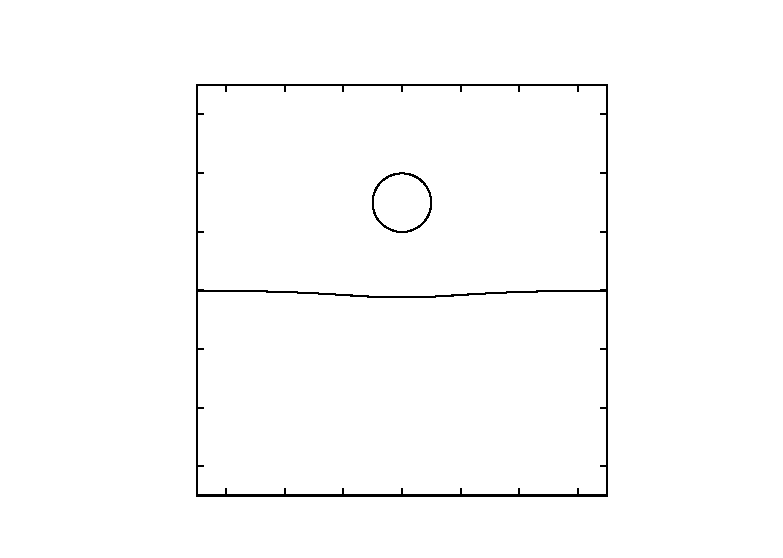
\includegraphics{../../Programming/sinking_bim_write_up/trunk/sinking_frame1}}%
    \gplfronttext
  \end{picture}%
\endgroup
}
        \caption{}
        \label{fig:sinking_frame1}
      \end{subfigure}
      ~
      \begin{subfigure}[b]{0.45\textwidth}
        \resizebox{\textwidth}{!}{\Large % GNUPLOT: LaTeX picture with Postscript
\begingroup
  \makeatletter
  \providecommand\color[2][]{%
    \GenericError{(gnuplot) \space\space\space\@spaces}{%
      Package color not loaded in conjunction with
      terminal option `colourtext'%
    }{See the gnuplot documentation for explanation.%
    }{Either use 'blacktext' in gnuplot or load the package
      color.sty in LaTeX.}%
    \renewcommand\color[2][]{}%
  }%
  \providecommand\includegraphics[2][]{%
    \GenericError{(gnuplot) \space\space\space\@spaces}{%
      Package graphicx or graphics not loaded%
    }{See the gnuplot documentation for explanation.%
    }{The gnuplot epslatex terminal needs graphicx.sty or graphics.sty.}%
    \renewcommand\includegraphics[2][]{}%
  }%
  \providecommand\rotatebox[2]{#2}%
  \@ifundefined{ifGPcolor}{%
    \newif\ifGPcolor
    \GPcolorfalse
  }{}%
  \@ifundefined{ifGPblacktext}{%
    \newif\ifGPblacktext
    \GPblacktexttrue
  }{}%
  % define a \g@addto@macro without @ in the name:
  \let\gplgaddtomacro\g@addto@macro
  % define empty templates for all commands taking text:
  \gdef\gplbacktext{}%
  \gdef\gplfronttext{}%
  \makeatother
  \ifGPblacktext
    % no textcolor at all
    \def\colorrgb#1{}%
    \def\colorgray#1{}%
  \else
    % gray or color?
    \ifGPcolor
      \def\colorrgb#1{\color[rgb]{#1}}%
      \def\colorgray#1{\color[gray]{#1}}%
      \expandafter\def\csname LTw\endcsname{\color{white}}%
      \expandafter\def\csname LTb\endcsname{\color{black}}%
      \expandafter\def\csname LTa\endcsname{\color{black}}%
      \expandafter\def\csname LT0\endcsname{\color[rgb]{1,0,0}}%
      \expandafter\def\csname LT1\endcsname{\color[rgb]{0,1,0}}%
      \expandafter\def\csname LT2\endcsname{\color[rgb]{0,0,1}}%
      \expandafter\def\csname LT3\endcsname{\color[rgb]{1,0,1}}%
      \expandafter\def\csname LT4\endcsname{\color[rgb]{0,1,1}}%
      \expandafter\def\csname LT5\endcsname{\color[rgb]{1,1,0}}%
      \expandafter\def\csname LT6\endcsname{\color[rgb]{0,0,0}}%
      \expandafter\def\csname LT7\endcsname{\color[rgb]{1,0.3,0}}%
      \expandafter\def\csname LT8\endcsname{\color[rgb]{0.5,0.5,0.5}}%
    \else
      % gray
      \def\colorrgb#1{\color{black}}%
      \def\colorgray#1{\color[gray]{#1}}%
      \expandafter\def\csname LTw\endcsname{\color{white}}%
      \expandafter\def\csname LTb\endcsname{\color{black}}%
      \expandafter\def\csname LTa\endcsname{\color{black}}%
      \expandafter\def\csname LT0\endcsname{\color{black}}%
      \expandafter\def\csname LT1\endcsname{\color{black}}%
      \expandafter\def\csname LT2\endcsname{\color{black}}%
      \expandafter\def\csname LT3\endcsname{\color{black}}%
      \expandafter\def\csname LT4\endcsname{\color{black}}%
      \expandafter\def\csname LT5\endcsname{\color{black}}%
      \expandafter\def\csname LT6\endcsname{\color{black}}%
      \expandafter\def\csname LT7\endcsname{\color{black}}%
      \expandafter\def\csname LT8\endcsname{\color{black}}%
    \fi
  \fi
    \setlength{\unitlength}{0.0500bp}%
    \ifx\gptboxheight\undefined%
      \newlength{\gptboxheight}%
      \newlength{\gptboxwidth}%
      \newsavebox{\gptboxtext}%
    \fi%
    \setlength{\fboxrule}{0.5pt}%
    \setlength{\fboxsep}{1pt}%
\begin{picture}(7200.00,5040.00)%
    \gplgaddtomacro\gplbacktext{%
      \csname LTb\endcsname%
      \put(1597,721){\makebox(0,0)[r]{\strut{}$-6$}}%
      \put(1597,1284){\makebox(0,0)[r]{\strut{}$-4$}}%
      \put(1597,1847){\makebox(0,0)[r]{\strut{}$-2$}}%
      \put(1597,2410){\makebox(0,0)[r]{\strut{}$0$}}%
      \put(1597,2972){\makebox(0,0)[r]{\strut{}$2$}}%
      \put(1597,3535){\makebox(0,0)[r]{\strut{}$4$}}%
      \put(1597,4098){\makebox(0,0)[r]{\strut{}$6$}}%
      \put(2010,220){\makebox(0,0){\strut{}$-6$}}%
      \put(2573,220){\makebox(0,0){\strut{}$-4$}}%
      \put(3136,220){\makebox(0,0){\strut{}$-2$}}%
      \put(3699,220){\makebox(0,0){\strut{}$0$}}%
      \put(4261,220){\makebox(0,0){\strut{}$2$}}%
      \put(4824,220){\makebox(0,0){\strut{}$4$}}%
      \put(5387,220){\makebox(0,0){\strut{}$6$}}%
    }%
    \gplgaddtomacro\gplfronttext{%
      \csname LTb\endcsname%
      \put(3698,4709){\makebox(0,0){\strut{}t = 10.74}}%
    }%
    \gplbacktext
    \put(0,0){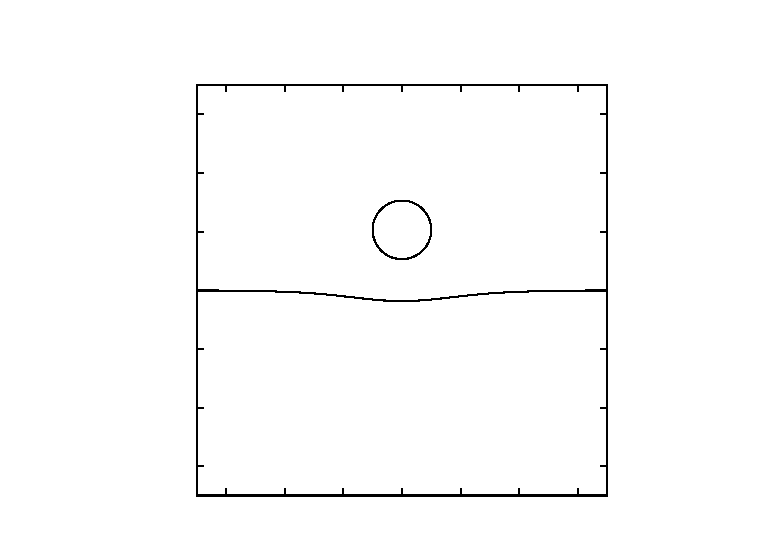
\includegraphics{../../Programming/sinking_bim_write_up/trunk/sinking_frame2}}%
    \gplfronttext
  \end{picture}%
\endgroup
}
        \caption{}
        \label{fig:sinking_frame2}
      \end{subfigure}
      
      \begin{subfigure}[b]{0.45\textwidth}
        \resizebox{\textwidth}{!}{\Large % GNUPLOT: LaTeX picture with Postscript
\begingroup
  \makeatletter
  \providecommand\color[2][]{%
    \GenericError{(gnuplot) \space\space\space\@spaces}{%
      Package color not loaded in conjunction with
      terminal option `colourtext'%
    }{See the gnuplot documentation for explanation.%
    }{Either use 'blacktext' in gnuplot or load the package
      color.sty in LaTeX.}%
    \renewcommand\color[2][]{}%
  }%
  \providecommand\includegraphics[2][]{%
    \GenericError{(gnuplot) \space\space\space\@spaces}{%
      Package graphicx or graphics not loaded%
    }{See the gnuplot documentation for explanation.%
    }{The gnuplot epslatex terminal needs graphicx.sty or graphics.sty.}%
    \renewcommand\includegraphics[2][]{}%
  }%
  \providecommand\rotatebox[2]{#2}%
  \@ifundefined{ifGPcolor}{%
    \newif\ifGPcolor
    \GPcolorfalse
  }{}%
  \@ifundefined{ifGPblacktext}{%
    \newif\ifGPblacktext
    \GPblacktexttrue
  }{}%
  % define a \g@addto@macro without @ in the name:
  \let\gplgaddtomacro\g@addto@macro
  % define empty templates for all commands taking text:
  \gdef\gplbacktext{}%
  \gdef\gplfronttext{}%
  \makeatother
  \ifGPblacktext
    % no textcolor at all
    \def\colorrgb#1{}%
    \def\colorgray#1{}%
  \else
    % gray or color?
    \ifGPcolor
      \def\colorrgb#1{\color[rgb]{#1}}%
      \def\colorgray#1{\color[gray]{#1}}%
      \expandafter\def\csname LTw\endcsname{\color{white}}%
      \expandafter\def\csname LTb\endcsname{\color{black}}%
      \expandafter\def\csname LTa\endcsname{\color{black}}%
      \expandafter\def\csname LT0\endcsname{\color[rgb]{1,0,0}}%
      \expandafter\def\csname LT1\endcsname{\color[rgb]{0,1,0}}%
      \expandafter\def\csname LT2\endcsname{\color[rgb]{0,0,1}}%
      \expandafter\def\csname LT3\endcsname{\color[rgb]{1,0,1}}%
      \expandafter\def\csname LT4\endcsname{\color[rgb]{0,1,1}}%
      \expandafter\def\csname LT5\endcsname{\color[rgb]{1,1,0}}%
      \expandafter\def\csname LT6\endcsname{\color[rgb]{0,0,0}}%
      \expandafter\def\csname LT7\endcsname{\color[rgb]{1,0.3,0}}%
      \expandafter\def\csname LT8\endcsname{\color[rgb]{0.5,0.5,0.5}}%
    \else
      % gray
      \def\colorrgb#1{\color{black}}%
      \def\colorgray#1{\color[gray]{#1}}%
      \expandafter\def\csname LTw\endcsname{\color{white}}%
      \expandafter\def\csname LTb\endcsname{\color{black}}%
      \expandafter\def\csname LTa\endcsname{\color{black}}%
      \expandafter\def\csname LT0\endcsname{\color{black}}%
      \expandafter\def\csname LT1\endcsname{\color{black}}%
      \expandafter\def\csname LT2\endcsname{\color{black}}%
      \expandafter\def\csname LT3\endcsname{\color{black}}%
      \expandafter\def\csname LT4\endcsname{\color{black}}%
      \expandafter\def\csname LT5\endcsname{\color{black}}%
      \expandafter\def\csname LT6\endcsname{\color{black}}%
      \expandafter\def\csname LT7\endcsname{\color{black}}%
      \expandafter\def\csname LT8\endcsname{\color{black}}%
    \fi
  \fi
    \setlength{\unitlength}{0.0500bp}%
    \ifx\gptboxheight\undefined%
      \newlength{\gptboxheight}%
      \newlength{\gptboxwidth}%
      \newsavebox{\gptboxtext}%
    \fi%
    \setlength{\fboxrule}{0.5pt}%
    \setlength{\fboxsep}{1pt}%
\begin{picture}(7200.00,5040.00)%
    \gplgaddtomacro\gplbacktext{%
      \csname LTb\endcsname%
      \put(1597,721){\makebox(0,0)[r]{\strut{}$-6$}}%
      \put(1597,1284){\makebox(0,0)[r]{\strut{}$-4$}}%
      \put(1597,1847){\makebox(0,0)[r]{\strut{}$-2$}}%
      \put(1597,2410){\makebox(0,0)[r]{\strut{}$0$}}%
      \put(1597,2972){\makebox(0,0)[r]{\strut{}$2$}}%
      \put(1597,3535){\makebox(0,0)[r]{\strut{}$4$}}%
      \put(1597,4098){\makebox(0,0)[r]{\strut{}$6$}}%
      \put(2010,220){\makebox(0,0){\strut{}$-6$}}%
      \put(2573,220){\makebox(0,0){\strut{}$-4$}}%
      \put(3136,220){\makebox(0,0){\strut{}$-2$}}%
      \put(3699,220){\makebox(0,0){\strut{}$0$}}%
      \put(4261,220){\makebox(0,0){\strut{}$2$}}%
      \put(4824,220){\makebox(0,0){\strut{}$4$}}%
      \put(5387,220){\makebox(0,0){\strut{}$6$}}%
    }%
    \gplgaddtomacro\gplfronttext{%
      \csname LTb\endcsname%
      \put(3698,4709){\makebox(0,0){\strut{}t = 12.64}}%
    }%
    \gplbacktext
    \put(0,0){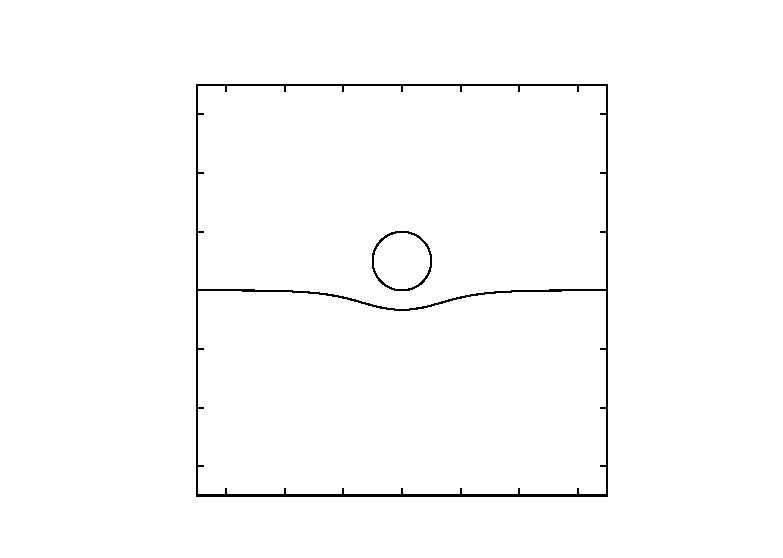
\includegraphics{sinking_frame3}}%
    \gplfronttext
  \end{picture}%
\endgroup
}
        \caption{}
        \label{fig:sinking_frame3}
      \end{subfigure}
      ~
      \begin{subfigure}[b]{0.45\textwidth}
        \resizebox{\textwidth}{!}{\Large % GNUPLOT: LaTeX picture with Postscript
\begingroup
  \makeatletter
  \providecommand\color[2][]{%
    \GenericError{(gnuplot) \space\space\space\@spaces}{%
      Package color not loaded in conjunction with
      terminal option `colourtext'%
    }{See the gnuplot documentation for explanation.%
    }{Either use 'blacktext' in gnuplot or load the package
      color.sty in LaTeX.}%
    \renewcommand\color[2][]{}%
  }%
  \providecommand\includegraphics[2][]{%
    \GenericError{(gnuplot) \space\space\space\@spaces}{%
      Package graphicx or graphics not loaded%
    }{See the gnuplot documentation for explanation.%
    }{The gnuplot epslatex terminal needs graphicx.sty or graphics.sty.}%
    \renewcommand\includegraphics[2][]{}%
  }%
  \providecommand\rotatebox[2]{#2}%
  \@ifundefined{ifGPcolor}{%
    \newif\ifGPcolor
    \GPcolorfalse
  }{}%
  \@ifundefined{ifGPblacktext}{%
    \newif\ifGPblacktext
    \GPblacktexttrue
  }{}%
  % define a \g@addto@macro without @ in the name:
  \let\gplgaddtomacro\g@addto@macro
  % define empty templates for all commands taking text:
  \gdef\gplbacktext{}%
  \gdef\gplfronttext{}%
  \makeatother
  \ifGPblacktext
    % no textcolor at all
    \def\colorrgb#1{}%
    \def\colorgray#1{}%
  \else
    % gray or color?
    \ifGPcolor
      \def\colorrgb#1{\color[rgb]{#1}}%
      \def\colorgray#1{\color[gray]{#1}}%
      \expandafter\def\csname LTw\endcsname{\color{white}}%
      \expandafter\def\csname LTb\endcsname{\color{black}}%
      \expandafter\def\csname LTa\endcsname{\color{black}}%
      \expandafter\def\csname LT0\endcsname{\color[rgb]{1,0,0}}%
      \expandafter\def\csname LT1\endcsname{\color[rgb]{0,1,0}}%
      \expandafter\def\csname LT2\endcsname{\color[rgb]{0,0,1}}%
      \expandafter\def\csname LT3\endcsname{\color[rgb]{1,0,1}}%
      \expandafter\def\csname LT4\endcsname{\color[rgb]{0,1,1}}%
      \expandafter\def\csname LT5\endcsname{\color[rgb]{1,1,0}}%
      \expandafter\def\csname LT6\endcsname{\color[rgb]{0,0,0}}%
      \expandafter\def\csname LT7\endcsname{\color[rgb]{1,0.3,0}}%
      \expandafter\def\csname LT8\endcsname{\color[rgb]{0.5,0.5,0.5}}%
    \else
      % gray
      \def\colorrgb#1{\color{black}}%
      \def\colorgray#1{\color[gray]{#1}}%
      \expandafter\def\csname LTw\endcsname{\color{white}}%
      \expandafter\def\csname LTb\endcsname{\color{black}}%
      \expandafter\def\csname LTa\endcsname{\color{black}}%
      \expandafter\def\csname LT0\endcsname{\color{black}}%
      \expandafter\def\csname LT1\endcsname{\color{black}}%
      \expandafter\def\csname LT2\endcsname{\color{black}}%
      \expandafter\def\csname LT3\endcsname{\color{black}}%
      \expandafter\def\csname LT4\endcsname{\color{black}}%
      \expandafter\def\csname LT5\endcsname{\color{black}}%
      \expandafter\def\csname LT6\endcsname{\color{black}}%
      \expandafter\def\csname LT7\endcsname{\color{black}}%
      \expandafter\def\csname LT8\endcsname{\color{black}}%
    \fi
  \fi
    \setlength{\unitlength}{0.0500bp}%
    \ifx\gptboxheight\undefined%
      \newlength{\gptboxheight}%
      \newlength{\gptboxwidth}%
      \newsavebox{\gptboxtext}%
    \fi%
    \setlength{\fboxrule}{0.5pt}%
    \setlength{\fboxsep}{1pt}%
\begin{picture}(7200.00,5040.00)%
    \gplgaddtomacro\gplbacktext{%
      \csname LTb\endcsname%
      \put(1597,721){\makebox(0,0)[r]{\strut{}$-6$}}%
      \put(1597,1284){\makebox(0,0)[r]{\strut{}$-4$}}%
      \put(1597,1847){\makebox(0,0)[r]{\strut{}$-2$}}%
      \put(1597,2410){\makebox(0,0)[r]{\strut{}$0$}}%
      \put(1597,2972){\makebox(0,0)[r]{\strut{}$2$}}%
      \put(1597,3535){\makebox(0,0)[r]{\strut{}$4$}}%
      \put(1597,4098){\makebox(0,0)[r]{\strut{}$6$}}%
      \put(2010,220){\makebox(0,0){\strut{}$-6$}}%
      \put(2573,220){\makebox(0,0){\strut{}$-4$}}%
      \put(3136,220){\makebox(0,0){\strut{}$-2$}}%
      \put(3699,220){\makebox(0,0){\strut{}$0$}}%
      \put(4261,220){\makebox(0,0){\strut{}$2$}}%
      \put(4824,220){\makebox(0,0){\strut{}$4$}}%
      \put(5387,220){\makebox(0,0){\strut{}$6$}}%
    }%
    \gplgaddtomacro\gplfronttext{%
      \csname LTb\endcsname%
      \put(3698,4709){\makebox(0,0){\strut{}t = 15.42}}%
    }%
    \gplbacktext
    \put(0,0){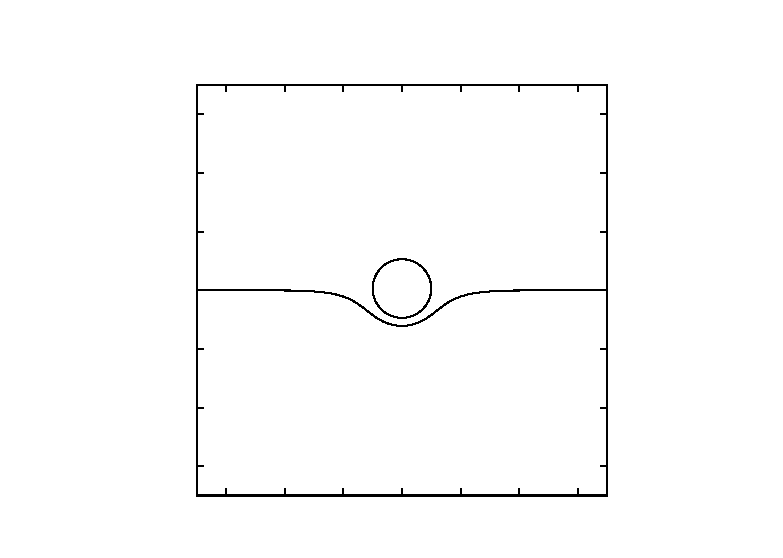
\includegraphics{sinking_frame4}}%
    \gplfronttext
  \end{picture}%
\endgroup
}
        \caption{}
        \label{fig:sinking_frame4}
      \end{subfigure}
      
      \begin{subfigure}[b]{0.45\textwidth}
        \resizebox{\textwidth}{!}{\Large % GNUPLOT: LaTeX picture with Postscript
\begingroup
  \makeatletter
  \providecommand\color[2][]{%
    \GenericError{(gnuplot) \space\space\space\@spaces}{%
      Package color not loaded in conjunction with
      terminal option `colourtext'%
    }{See the gnuplot documentation for explanation.%
    }{Either use 'blacktext' in gnuplot or load the package
      color.sty in LaTeX.}%
    \renewcommand\color[2][]{}%
  }%
  \providecommand\includegraphics[2][]{%
    \GenericError{(gnuplot) \space\space\space\@spaces}{%
      Package graphicx or graphics not loaded%
    }{See the gnuplot documentation for explanation.%
    }{The gnuplot epslatex terminal needs graphicx.sty or graphics.sty.}%
    \renewcommand\includegraphics[2][]{}%
  }%
  \providecommand\rotatebox[2]{#2}%
  \@ifundefined{ifGPcolor}{%
    \newif\ifGPcolor
    \GPcolorfalse
  }{}%
  \@ifundefined{ifGPblacktext}{%
    \newif\ifGPblacktext
    \GPblacktexttrue
  }{}%
  % define a \g@addto@macro without @ in the name:
  \let\gplgaddtomacro\g@addto@macro
  % define empty templates for all commands taking text:
  \gdef\gplbacktext{}%
  \gdef\gplfronttext{}%
  \makeatother
  \ifGPblacktext
    % no textcolor at all
    \def\colorrgb#1{}%
    \def\colorgray#1{}%
  \else
    % gray or color?
    \ifGPcolor
      \def\colorrgb#1{\color[rgb]{#1}}%
      \def\colorgray#1{\color[gray]{#1}}%
      \expandafter\def\csname LTw\endcsname{\color{white}}%
      \expandafter\def\csname LTb\endcsname{\color{black}}%
      \expandafter\def\csname LTa\endcsname{\color{black}}%
      \expandafter\def\csname LT0\endcsname{\color[rgb]{1,0,0}}%
      \expandafter\def\csname LT1\endcsname{\color[rgb]{0,1,0}}%
      \expandafter\def\csname LT2\endcsname{\color[rgb]{0,0,1}}%
      \expandafter\def\csname LT3\endcsname{\color[rgb]{1,0,1}}%
      \expandafter\def\csname LT4\endcsname{\color[rgb]{0,1,1}}%
      \expandafter\def\csname LT5\endcsname{\color[rgb]{1,1,0}}%
      \expandafter\def\csname LT6\endcsname{\color[rgb]{0,0,0}}%
      \expandafter\def\csname LT7\endcsname{\color[rgb]{1,0.3,0}}%
      \expandafter\def\csname LT8\endcsname{\color[rgb]{0.5,0.5,0.5}}%
    \else
      % gray
      \def\colorrgb#1{\color{black}}%
      \def\colorgray#1{\color[gray]{#1}}%
      \expandafter\def\csname LTw\endcsname{\color{white}}%
      \expandafter\def\csname LTb\endcsname{\color{black}}%
      \expandafter\def\csname LTa\endcsname{\color{black}}%
      \expandafter\def\csname LT0\endcsname{\color{black}}%
      \expandafter\def\csname LT1\endcsname{\color{black}}%
      \expandafter\def\csname LT2\endcsname{\color{black}}%
      \expandafter\def\csname LT3\endcsname{\color{black}}%
      \expandafter\def\csname LT4\endcsname{\color{black}}%
      \expandafter\def\csname LT5\endcsname{\color{black}}%
      \expandafter\def\csname LT6\endcsname{\color{black}}%
      \expandafter\def\csname LT7\endcsname{\color{black}}%
      \expandafter\def\csname LT8\endcsname{\color{black}}%
    \fi
  \fi
    \setlength{\unitlength}{0.0500bp}%
    \ifx\gptboxheight\undefined%
      \newlength{\gptboxheight}%
      \newlength{\gptboxwidth}%
      \newsavebox{\gptboxtext}%
    \fi%
    \setlength{\fboxrule}{0.5pt}%
    \setlength{\fboxsep}{1pt}%
\begin{picture}(7200.00,5040.00)%
    \gplgaddtomacro\gplbacktext{%
      \csname LTb\endcsname%
      \put(1597,721){\makebox(0,0)[r]{\strut{}$-6$}}%
      \put(1597,1284){\makebox(0,0)[r]{\strut{}$-4$}}%
      \put(1597,1847){\makebox(0,0)[r]{\strut{}$-2$}}%
      \put(1597,2410){\makebox(0,0)[r]{\strut{}$0$}}%
      \put(1597,2972){\makebox(0,0)[r]{\strut{}$2$}}%
      \put(1597,3535){\makebox(0,0)[r]{\strut{}$4$}}%
      \put(1597,4098){\makebox(0,0)[r]{\strut{}$6$}}%
      \put(2010,220){\makebox(0,0){\strut{}$-6$}}%
      \put(2573,220){\makebox(0,0){\strut{}$-4$}}%
      \put(3136,220){\makebox(0,0){\strut{}$-2$}}%
      \put(3699,220){\makebox(0,0){\strut{}$0$}}%
      \put(4261,220){\makebox(0,0){\strut{}$2$}}%
      \put(4824,220){\makebox(0,0){\strut{}$4$}}%
      \put(5387,220){\makebox(0,0){\strut{}$6$}}%
    }%
    \gplgaddtomacro\gplfronttext{%
      \csname LTb\endcsname%
      \put(3698,4709){\makebox(0,0){\strut{}t = 30.84}}%
    }%
    \gplbacktext
    \put(0,0){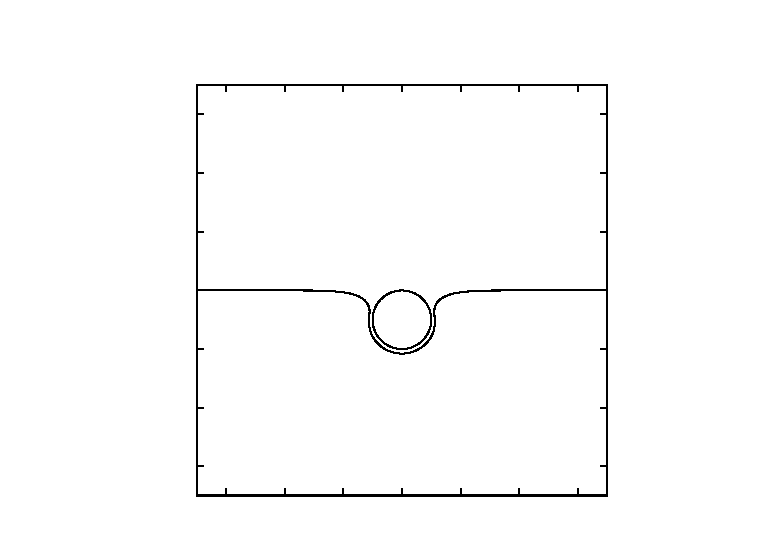
\includegraphics{../../Programming/sinking_bim_write_up/trunk/sinking_frame5}}%
    \gplfronttext
  \end{picture}%
\endgroup
}
        \caption{}
        \label{fig:sinking_frame5}
      \end{subfigure}
      ~
      \begin{subfigure}[b]{0.45\textwidth}
        \resizebox{\textwidth}{!}{\large % GNUPLOT: LaTeX picture with Postscript
\begingroup
  \makeatletter
  \providecommand\color[2][]{%
    \GenericError{(gnuplot) \space\space\space\@spaces}{%
      Package color not loaded in conjunction with
      terminal option `colourtext'%
    }{See the gnuplot documentation for explanation.%
    }{Either use 'blacktext' in gnuplot or load the package
      color.sty in LaTeX.}%
    \renewcommand\color[2][]{}%
  }%
  \providecommand\includegraphics[2][]{%
    \GenericError{(gnuplot) \space\space\space\@spaces}{%
      Package graphicx or graphics not loaded%
    }{See the gnuplot documentation for explanation.%
    }{The gnuplot epslatex terminal needs graphicx.sty or graphics.sty.}%
    \renewcommand\includegraphics[2][]{}%
  }%
  \providecommand\rotatebox[2]{#2}%
  \@ifundefined{ifGPcolor}{%
    \newif\ifGPcolor
    \GPcolorfalse
  }{}%
  \@ifundefined{ifGPblacktext}{%
    \newif\ifGPblacktext
    \GPblacktexttrue
  }{}%
  % define a \g@addto@macro without @ in the name:
  \let\gplgaddtomacro\g@addto@macro
  % define empty templates for all commands taking text:
  \gdef\gplbacktext{}%
  \gdef\gplfronttext{}%
  \makeatother
  \ifGPblacktext
    % no textcolor at all
    \def\colorrgb#1{}%
    \def\colorgray#1{}%
  \else
    % gray or color?
    \ifGPcolor
      \def\colorrgb#1{\color[rgb]{#1}}%
      \def\colorgray#1{\color[gray]{#1}}%
      \expandafter\def\csname LTw\endcsname{\color{white}}%
      \expandafter\def\csname LTb\endcsname{\color{black}}%
      \expandafter\def\csname LTa\endcsname{\color{black}}%
      \expandafter\def\csname LT0\endcsname{\color[rgb]{1,0,0}}%
      \expandafter\def\csname LT1\endcsname{\color[rgb]{0,1,0}}%
      \expandafter\def\csname LT2\endcsname{\color[rgb]{0,0,1}}%
      \expandafter\def\csname LT3\endcsname{\color[rgb]{1,0,1}}%
      \expandafter\def\csname LT4\endcsname{\color[rgb]{0,1,1}}%
      \expandafter\def\csname LT5\endcsname{\color[rgb]{1,1,0}}%
      \expandafter\def\csname LT6\endcsname{\color[rgb]{0,0,0}}%
      \expandafter\def\csname LT7\endcsname{\color[rgb]{1,0.3,0}}%
      \expandafter\def\csname LT8\endcsname{\color[rgb]{0.5,0.5,0.5}}%
    \else
      % gray
      \def\colorrgb#1{\color{black}}%
      \def\colorgray#1{\color[gray]{#1}}%
      \expandafter\def\csname LTw\endcsname{\color{white}}%
      \expandafter\def\csname LTb\endcsname{\color{black}}%
      \expandafter\def\csname LTa\endcsname{\color{black}}%
      \expandafter\def\csname LT0\endcsname{\color{black}}%
      \expandafter\def\csname LT1\endcsname{\color{black}}%
      \expandafter\def\csname LT2\endcsname{\color{black}}%
      \expandafter\def\csname LT3\endcsname{\color{black}}%
      \expandafter\def\csname LT4\endcsname{\color{black}}%
      \expandafter\def\csname LT5\endcsname{\color{black}}%
      \expandafter\def\csname LT6\endcsname{\color{black}}%
      \expandafter\def\csname LT7\endcsname{\color{black}}%
      \expandafter\def\csname LT8\endcsname{\color{black}}%
    \fi
  \fi
    \setlength{\unitlength}{0.0500bp}%
    \ifx\gptboxheight\undefined%
      \newlength{\gptboxheight}%
      \newlength{\gptboxwidth}%
      \newsavebox{\gptboxtext}%
    \fi%
    \setlength{\fboxrule}{0.5pt}%
    \setlength{\fboxsep}{1pt}%
\begin{picture}(7200.00,5040.00)%
    \gplgaddtomacro\gplbacktext{%
      \csname LTb\endcsname%
      \put(1597,721){\makebox(0,0)[r]{\strut{}$-6$}}%
      \put(1597,1284){\makebox(0,0)[r]{\strut{}$-4$}}%
      \put(1597,1847){\makebox(0,0)[r]{\strut{}$-2$}}%
      \put(1597,2410){\makebox(0,0)[r]{\strut{}$0$}}%
      \put(1597,2972){\makebox(0,0)[r]{\strut{}$2$}}%
      \put(1597,3535){\makebox(0,0)[r]{\strut{}$4$}}%
      \put(1597,4098){\makebox(0,0)[r]{\strut{}$6$}}%
      \put(2010,220){\makebox(0,0){\strut{}$-6$}}%
      \put(2573,220){\makebox(0,0){\strut{}$-4$}}%
      \put(3136,220){\makebox(0,0){\strut{}$-2$}}%
      \put(3699,220){\makebox(0,0){\strut{}$0$}}%
      \put(4261,220){\makebox(0,0){\strut{}$2$}}%
      \put(4824,220){\makebox(0,0){\strut{}$4$}}%
      \put(5387,220){\makebox(0,0){\strut{}$6$}}%
    }%
    \gplgaddtomacro\gplfronttext{%
      \csname LTb\endcsname%
      \put(3698,4709){\makebox(0,0){\strut{}t = 58.19}}%
    }%
    \gplbacktext
    \put(0,0){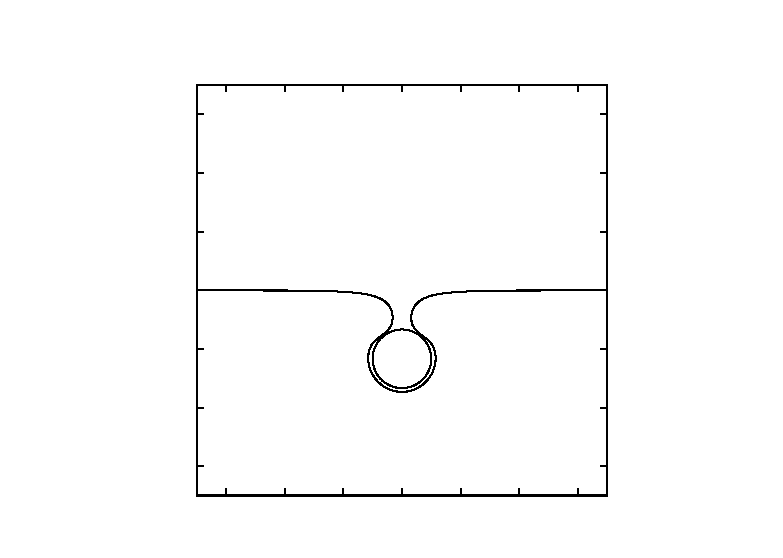
\includegraphics{sinking_frame6}}%
    \gplfronttext
  \end{picture}%
\endgroup
}
        \caption{}
        \label{fig:sinking_frame6}
      \end{subfigure}
      \caption{Settling of a sphere onto and through the interface when $D = 2.2$, $\Bo = 3.5$ and $\lambda = 1$. The interface deforms as the sphere approaches and envelopes the sphere as it sinks.}\label{fig:sinking_frame}
    \end{figure}

  \begin{figure}
    \resizebox{0.9\textwidth}{!}{\Large % GNUPLOT: LaTeX picture with Postscript
\begingroup
  \makeatletter
  \providecommand\color[2][]{%
    \GenericError{(gnuplot) \space\space\space\@spaces}{%
      Package color not loaded in conjunction with
      terminal option `colourtext'%
    }{See the gnuplot documentation for explanation.%
    }{Either use 'blacktext' in gnuplot or load the package
      color.sty in LaTeX.}%
    \renewcommand\color[2][]{}%
  }%
  \providecommand\includegraphics[2][]{%
    \GenericError{(gnuplot) \space\space\space\@spaces}{%
      Package graphicx or graphics not loaded%
    }{See the gnuplot documentation for explanation.%
    }{The gnuplot epslatex terminal needs graphicx.sty or graphics.sty.}%
    \renewcommand\includegraphics[2][]{}%
  }%
  \providecommand\rotatebox[2]{#2}%
  \@ifundefined{ifGPcolor}{%
    \newif\ifGPcolor
    \GPcolorfalse
  }{}%
  \@ifundefined{ifGPblacktext}{%
    \newif\ifGPblacktext
    \GPblacktexttrue
  }{}%
  % define a \g@addto@macro without @ in the name:
  \let\gplgaddtomacro\g@addto@macro
  % define empty templates for all commands taking text:
  \gdef\gplbacktext{}%
  \gdef\gplfronttext{}%
  \makeatother
  \ifGPblacktext
    % no textcolor at all
    \def\colorrgb#1{}%
    \def\colorgray#1{}%
  \else
    % gray or color?
    \ifGPcolor
      \def\colorrgb#1{\color[rgb]{#1}}%
      \def\colorgray#1{\color[gray]{#1}}%
      \expandafter\def\csname LTw\endcsname{\color{white}}%
      \expandafter\def\csname LTb\endcsname{\color{black}}%
      \expandafter\def\csname LTa\endcsname{\color{black}}%
      \expandafter\def\csname LT0\endcsname{\color[rgb]{1,0,0}}%
      \expandafter\def\csname LT1\endcsname{\color[rgb]{0,1,0}}%
      \expandafter\def\csname LT2\endcsname{\color[rgb]{0,0,1}}%
      \expandafter\def\csname LT3\endcsname{\color[rgb]{1,0,1}}%
      \expandafter\def\csname LT4\endcsname{\color[rgb]{0,1,1}}%
      \expandafter\def\csname LT5\endcsname{\color[rgb]{1,1,0}}%
      \expandafter\def\csname LT6\endcsname{\color[rgb]{0,0,0}}%
      \expandafter\def\csname LT7\endcsname{\color[rgb]{1,0.3,0}}%
      \expandafter\def\csname LT8\endcsname{\color[rgb]{0.5,0.5,0.5}}%
    \else
      % gray
      \def\colorrgb#1{\color{black}}%
      \def\colorgray#1{\color[gray]{#1}}%
      \expandafter\def\csname LTw\endcsname{\color{white}}%
      \expandafter\def\csname LTb\endcsname{\color{black}}%
      \expandafter\def\csname LTa\endcsname{\color{black}}%
      \expandafter\def\csname LT0\endcsname{\color{black}}%
      \expandafter\def\csname LT1\endcsname{\color{black}}%
      \expandafter\def\csname LT2\endcsname{\color{black}}%
      \expandafter\def\csname LT3\endcsname{\color{black}}%
      \expandafter\def\csname LT4\endcsname{\color{black}}%
      \expandafter\def\csname LT5\endcsname{\color{black}}%
      \expandafter\def\csname LT6\endcsname{\color{black}}%
      \expandafter\def\csname LT7\endcsname{\color{black}}%
      \expandafter\def\csname LT8\endcsname{\color{black}}%
    \fi
  \fi
    \setlength{\unitlength}{0.0500bp}%
    \ifx\gptboxheight\undefined%
      \newlength{\gptboxheight}%
      \newlength{\gptboxwidth}%
      \newsavebox{\gptboxtext}%
    \fi%
    \setlength{\fboxrule}{0.5pt}%
    \setlength{\fboxsep}{1pt}%
\begin{picture}(7200.00,5040.00)%
    \gplgaddtomacro\gplbacktext{%
      \csname LTb\endcsname%
      \put(682,704){\makebox(0,0)[r]{\strut{}$-4$}}%
      \put(682,1213){\makebox(0,0)[r]{\strut{}$-2$}}%
      \put(682,1722){\makebox(0,0)[r]{\strut{}$0$}}%
      \put(682,2231){\makebox(0,0)[r]{\strut{}$2$}}%
      \put(682,2740){\makebox(0,0)[r]{\strut{}$4$}}%
      \put(682,3248){\makebox(0,0)[r]{\strut{}$6$}}%
      \put(682,3757){\makebox(0,0)[r]{\strut{}$8$}}%
      \put(682,4266){\makebox(0,0)[r]{\strut{}$10$}}%
      \put(682,4775){\makebox(0,0)[r]{\strut{}$12$}}%
      \put(814,484){\makebox(0,0){\strut{}$0$}}%
      \put(1812,484){\makebox(0,0){\strut{}$10$}}%
      \put(2810,484){\makebox(0,0){\strut{}$20$}}%
      \put(3809,484){\makebox(0,0){\strut{}$30$}}%
      \put(4807,484){\makebox(0,0){\strut{}$40$}}%
      \put(5805,484){\makebox(0,0){\strut{}$50$}}%
      \put(6803,484){\makebox(0,0){\strut{}$60$}}%
    }%
    \gplgaddtomacro\gplfronttext{%
      \csname LTb\endcsname%
      \put(176,2739){\rotatebox{-270}{\makebox(0,0){\strut{}$z_{\text{s}}$}}}%
      \put(3808,154){\makebox(0,0){\strut{}$t$}}%
    }%
    \gplbacktext
    \put(0,0){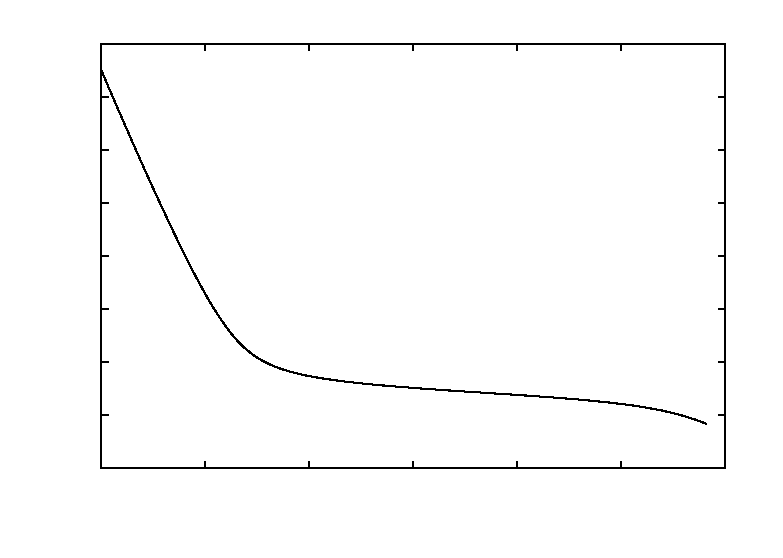
\includegraphics{sinking_traj}}%
    \gplfronttext
  \end{picture}%
\endgroup
}
    \caption{Position curve of the sphere, which is seen to slow down at the interface, before accelerating away.\label{fig:sinking_traj}}
  \end{figure}

A regime diagram has been constructed for the floating-sinking transition. It has been found that for $\lambda \leq 10$ the location of the transition in the parameter space defined by $D$, $\Bo$ and $\lambda$ is independent of $\lambda$. Figure~\ref{fig:regime} shows the transition in a plane of constant $\lambda$ over orders of magnitude variation in $D$ and $\Bo$. Also shown is the prediction for this transition from the theoretical model of \citep{Vella06}. This model finds the maximum $D$ for a given $\Bo$ and contact angle for a sphere to be at equilibrium at an interface. This is different from our model, since no initial motion of the sphere is considered, and the existence of a contact line on the sphere is imposed. Despite these differences, we see that the results in figure~\ref{fig:regime} agree with this model. In figure~\ref{fig:zoom_regime} however, we show the results of a denser investigation of the paramter space, in the region where the transition curve has the highest curvature. It can be seen that although our model reproduces the shape of the predicted regime boundary, there is an offset such that our model predicts a higher maximum value of $D$ for a given $\Bo$.

  \begin{figure}
    \resizebox{0.9\textwidth}{!}{\large % GNUPLOT: LaTeX picture with Postscript
\begingroup
  \makeatletter
  \providecommand\color[2][]{%
    \GenericError{(gnuplot) \space\space\space\@spaces}{%
      Package color not loaded in conjunction with
      terminal option `colourtext'%
    }{See the gnuplot documentation for explanation.%
    }{Either use 'blacktext' in gnuplot or load the package
      color.sty in LaTeX.}%
    \renewcommand\color[2][]{}%
  }%
  \providecommand\includegraphics[2][]{%
    \GenericError{(gnuplot) \space\space\space\@spaces}{%
      Package graphicx or graphics not loaded%
    }{See the gnuplot documentation for explanation.%
    }{The gnuplot epslatex terminal needs graphicx.sty or graphics.sty.}%
    \renewcommand\includegraphics[2][]{}%
  }%
  \providecommand\rotatebox[2]{#2}%
  \@ifundefined{ifGPcolor}{%
    \newif\ifGPcolor
    \GPcolorfalse
  }{}%
  \@ifundefined{ifGPblacktext}{%
    \newif\ifGPblacktext
    \GPblacktexttrue
  }{}%
  % define a \g@addto@macro without @ in the name:
  \let\gplgaddtomacro\g@addto@macro
  % define empty templates for all commands taking text:
  \gdef\gplbacktext{}%
  \gdef\gplfronttext{}%
  \makeatother
  \ifGPblacktext
    % no textcolor at all
    \def\colorrgb#1{}%
    \def\colorgray#1{}%
  \else
    % gray or color?
    \ifGPcolor
      \def\colorrgb#1{\color[rgb]{#1}}%
      \def\colorgray#1{\color[gray]{#1}}%
      \expandafter\def\csname LTw\endcsname{\color{white}}%
      \expandafter\def\csname LTb\endcsname{\color{black}}%
      \expandafter\def\csname LTa\endcsname{\color{black}}%
      \expandafter\def\csname LT0\endcsname{\color[rgb]{1,0,0}}%
      \expandafter\def\csname LT1\endcsname{\color[rgb]{0,1,0}}%
      \expandafter\def\csname LT2\endcsname{\color[rgb]{0,0,1}}%
      \expandafter\def\csname LT3\endcsname{\color[rgb]{1,0,1}}%
      \expandafter\def\csname LT4\endcsname{\color[rgb]{0,1,1}}%
      \expandafter\def\csname LT5\endcsname{\color[rgb]{1,1,0}}%
      \expandafter\def\csname LT6\endcsname{\color[rgb]{0,0,0}}%
      \expandafter\def\csname LT7\endcsname{\color[rgb]{1,0.3,0}}%
      \expandafter\def\csname LT8\endcsname{\color[rgb]{0.5,0.5,0.5}}%
    \else
      % gray
      \def\colorrgb#1{\color{black}}%
      \def\colorgray#1{\color[gray]{#1}}%
      \expandafter\def\csname LTw\endcsname{\color{white}}%
      \expandafter\def\csname LTb\endcsname{\color{black}}%
      \expandafter\def\csname LTa\endcsname{\color{black}}%
      \expandafter\def\csname LT0\endcsname{\color{black}}%
      \expandafter\def\csname LT1\endcsname{\color{black}}%
      \expandafter\def\csname LT2\endcsname{\color{black}}%
      \expandafter\def\csname LT3\endcsname{\color{black}}%
      \expandafter\def\csname LT4\endcsname{\color{black}}%
      \expandafter\def\csname LT5\endcsname{\color{black}}%
      \expandafter\def\csname LT6\endcsname{\color{black}}%
      \expandafter\def\csname LT7\endcsname{\color{black}}%
      \expandafter\def\csname LT8\endcsname{\color{black}}%
    \fi
  \fi
    \setlength{\unitlength}{0.0500bp}%
    \ifx\gptboxheight\undefined%
      \newlength{\gptboxheight}%
      \newlength{\gptboxwidth}%
      \newsavebox{\gptboxtext}%
    \fi%
    \setlength{\fboxrule}{0.5pt}%
    \setlength{\fboxsep}{1pt}%
\begin{picture}(7200.00,5040.00)%
    \gplgaddtomacro\gplbacktext{%
      \csname LTb\endcsname%
      \put(1078,924){\makebox(0,0)[r]{\strut{}$0.1$}}%
      \put(1078,1615){\makebox(0,0)[r]{\strut{}$1$}}%
      \put(1078,2306){\makebox(0,0)[r]{\strut{}$10$}}%
      \put(1078,2997){\makebox(0,0)[r]{\strut{}$100$}}%
      \put(1078,3688){\makebox(0,0)[r]{\strut{}$1000$}}%
      \put(1078,4379){\makebox(0,0)[r]{\strut{}$10000$}}%
      \put(1210,704){\makebox(0,0){\strut{}$0.001$}}%
      \put(2009,704){\makebox(0,0){\strut{}$0.01$}}%
      \put(2808,704){\makebox(0,0){\strut{}$0.1$}}%
      \put(3607,704){\makebox(0,0){\strut{}$1$}}%
      \put(4406,704){\makebox(0,0){\strut{}$10$}}%
      \put(5205,704){\makebox(0,0){\strut{}$100$}}%
      \put(6004,704){\makebox(0,0){\strut{}$1000$}}%
      \put(6803,704){\makebox(0,0){\strut{}$10000$}}%
    }%
    \gplgaddtomacro\gplfronttext{%
      \csname LTb\endcsname%
      \put(176,2651){\rotatebox{-270}{\makebox(0,0){\strut{}$D$}}}%
      \put(4006,374){\makebox(0,0){\strut{}$\text{Bo}$}}%
      \put(4006,4709){\makebox(0,0){\strut{}$\lambda = 1$}}%
      \csname LTb\endcsname%
      \put(2064,173){\makebox(0,0)[r]{\strut{}Floating}}%
      \csname LTb\endcsname%
      \put(4239,173){\makebox(0,0)[r]{\strut{}Sinking}}%
      \csname LTb\endcsname%
      \put(6414,173){\makebox(0,0)[r]{\strut{}Vella 2006}}%
    }%
    \gplbacktext
    \put(0,0){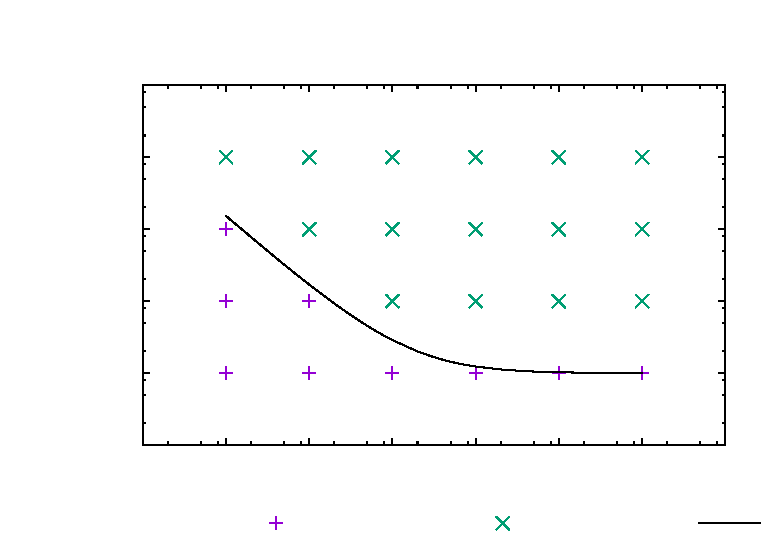
\includegraphics{regime_pub}}%
    \gplfronttext
  \end{picture}%
\endgroup
}
    \caption{A regime diagram showing the fields of floating and sinking in the $\lambda = 1$ plane of the parameters space defined by ${\lambda, \Bo, D}$. Points show results of simulations. Solid line shows prediction from theoretical model of \citep{Vella06}.\label{fig:regime}}
  \end{figure}

  \begin{figure}
    \resizebox{0.9\textwidth}{!}{\large % GNUPLOT: LaTeX picture with Postscript
\begingroup
  \makeatletter
  \providecommand\color[2][]{%
    \GenericError{(gnuplot) \space\space\space\@spaces}{%
      Package color not loaded in conjunction with
      terminal option `colourtext'%
    }{See the gnuplot documentation for explanation.%
    }{Either use 'blacktext' in gnuplot or load the package
      color.sty in LaTeX.}%
    \renewcommand\color[2][]{}%
  }%
  \providecommand\includegraphics[2][]{%
    \GenericError{(gnuplot) \space\space\space\@spaces}{%
      Package graphicx or graphics not loaded%
    }{See the gnuplot documentation for explanation.%
    }{The gnuplot epslatex terminal needs graphicx.sty or graphics.sty.}%
    \renewcommand\includegraphics[2][]{}%
  }%
  \providecommand\rotatebox[2]{#2}%
  \@ifundefined{ifGPcolor}{%
    \newif\ifGPcolor
    \GPcolorfalse
  }{}%
  \@ifundefined{ifGPblacktext}{%
    \newif\ifGPblacktext
    \GPblacktexttrue
  }{}%
  % define a \g@addto@macro without @ in the name:
  \let\gplgaddtomacro\g@addto@macro
  % define empty templates for all commands taking text:
  \gdef\gplbacktext{}%
  \gdef\gplfronttext{}%
  \makeatother
  \ifGPblacktext
    % no textcolor at all
    \def\colorrgb#1{}%
    \def\colorgray#1{}%
  \else
    % gray or color?
    \ifGPcolor
      \def\colorrgb#1{\color[rgb]{#1}}%
      \def\colorgray#1{\color[gray]{#1}}%
      \expandafter\def\csname LTw\endcsname{\color{white}}%
      \expandafter\def\csname LTb\endcsname{\color{black}}%
      \expandafter\def\csname LTa\endcsname{\color{black}}%
      \expandafter\def\csname LT0\endcsname{\color[rgb]{1,0,0}}%
      \expandafter\def\csname LT1\endcsname{\color[rgb]{0,1,0}}%
      \expandafter\def\csname LT2\endcsname{\color[rgb]{0,0,1}}%
      \expandafter\def\csname LT3\endcsname{\color[rgb]{1,0,1}}%
      \expandafter\def\csname LT4\endcsname{\color[rgb]{0,1,1}}%
      \expandafter\def\csname LT5\endcsname{\color[rgb]{1,1,0}}%
      \expandafter\def\csname LT6\endcsname{\color[rgb]{0,0,0}}%
      \expandafter\def\csname LT7\endcsname{\color[rgb]{1,0.3,0}}%
      \expandafter\def\csname LT8\endcsname{\color[rgb]{0.5,0.5,0.5}}%
    \else
      % gray
      \def\colorrgb#1{\color{black}}%
      \def\colorgray#1{\color[gray]{#1}}%
      \expandafter\def\csname LTw\endcsname{\color{white}}%
      \expandafter\def\csname LTb\endcsname{\color{black}}%
      \expandafter\def\csname LTa\endcsname{\color{black}}%
      \expandafter\def\csname LT0\endcsname{\color{black}}%
      \expandafter\def\csname LT1\endcsname{\color{black}}%
      \expandafter\def\csname LT2\endcsname{\color{black}}%
      \expandafter\def\csname LT3\endcsname{\color{black}}%
      \expandafter\def\csname LT4\endcsname{\color{black}}%
      \expandafter\def\csname LT5\endcsname{\color{black}}%
      \expandafter\def\csname LT6\endcsname{\color{black}}%
      \expandafter\def\csname LT7\endcsname{\color{black}}%
      \expandafter\def\csname LT8\endcsname{\color{black}}%
    \fi
  \fi
    \setlength{\unitlength}{0.0500bp}%
    \ifx\gptboxheight\undefined%
      \newlength{\gptboxheight}%
      \newlength{\gptboxwidth}%
      \newsavebox{\gptboxtext}%
    \fi%
    \setlength{\fboxrule}{0.5pt}%
    \setlength{\fboxsep}{1pt}%
\begin{picture}(7200.00,5040.00)%
    \gplgaddtomacro\gplbacktext{%
      \csname LTb\endcsname%
      \put(550,924){\makebox(0,0)[r]{\strut{}$0$}}%
      \put(550,1615){\makebox(0,0)[r]{\strut{}$1$}}%
      \put(550,2306){\makebox(0,0)[r]{\strut{}$2$}}%
      \put(550,2997){\makebox(0,0)[r]{\strut{}$3$}}%
      \put(550,3688){\makebox(0,0)[r]{\strut{}$4$}}%
      \put(550,4379){\makebox(0,0)[r]{\strut{}$5$}}%
      \put(682,704){\makebox(0,0){\strut{}$0$}}%
      \put(1906,704){\makebox(0,0){\strut{}$2$}}%
      \put(3130,704){\makebox(0,0){\strut{}$4$}}%
      \put(4355,704){\makebox(0,0){\strut{}$6$}}%
      \put(5579,704){\makebox(0,0){\strut{}$8$}}%
      \put(6803,704){\makebox(0,0){\strut{}$10$}}%
    }%
    \gplgaddtomacro\gplfronttext{%
      \csname LTb\endcsname%
      \put(176,2651){\rotatebox{-270}{\makebox(0,0){\strut{}$D$}}}%
      \put(3742,374){\makebox(0,0){\strut{}$\text{Bo}$}}%
      \put(3742,4709){\makebox(0,0){\strut{}$\lambda = 1$}}%
      \csname LTb\endcsname%
      \put(1800,173){\makebox(0,0)[r]{\strut{}Floating}}%
      \csname LTb\endcsname%
      \put(3975,173){\makebox(0,0)[r]{\strut{}Sinking}}%
      \csname LTb\endcsname%
      \put(6150,173){\makebox(0,0)[r]{\strut{}Vella 2006}}%
    }%
    \gplbacktext
    \put(0,0){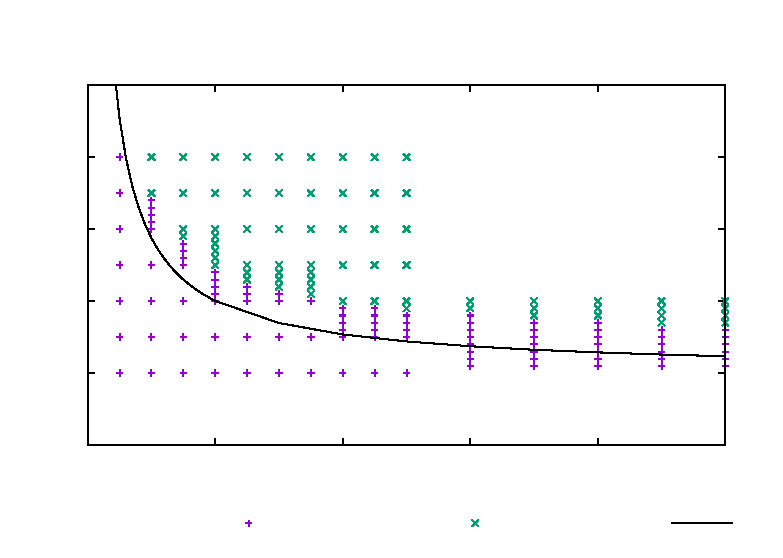
\includegraphics{zoom_regime_pub}}%
    \gplfronttext
  \end{picture}%
\endgroup
}
    \caption{A regime diagram showing the fields of floating and sinking in the $\lambda = 1$ plane of the parameters space defined by ${\lambda, \Bo, D}$. Points show results of simulations. Solid line shows prediction from theoretical model of \citep{Vella06}.\label{fig:zoom_regime}}
  \end{figure}

\subsubsection{Equilibrium Floating Position}
\label{subsubsec:equilib_pos}

For simulations where the sphere is observed to attain a static equilibrium position, the dependence of the final height of the sphere $z_{\text{eq}}$on $D$, $\Bo$ and $\lambda$ has been determined. A key result is that $z_{\text{eq}}$ is independent of the viscosity ratio as seen in figure~\ref{fig:fin_pos_viscos}. Figure~\ref{fig:fin_pos} shows the dependence of $z_{\text{eq}}$ on $\Bo$ for different values of $D$. There are a number of points to note here. Firstly, as $\Bo \to 0$, the dependence of $z_{\text{eq}}$ on $D$ vanishes, and $z_{\text{c}} \to 0$. Once $\Bo > 0.01$, $z_{\text{c}}$ decreases and the equilibrium position of sphere is deeper with respect to the plane of the undeformed interface. For a given $\Bo$, the larger the value of $D$, the deeper the equilibrium position of the sphere. For $D \neq 1$, as $\Bo$ increases the floating-sinking transition is crossed and $z_{\text{eq}} \to -\infty$. For $D = 1$, as $\Bo \to \infty$, $z_{\text{c}} \to -0.32$. 

  \begin{figure}
    \resizebox{0.9\textwidth}{!}{\large % GNUPLOT: LaTeX picture with Postscript
\begingroup
  \makeatletter
  \providecommand\color[2][]{%
    \GenericError{(gnuplot) \space\space\space\@spaces}{%
      Package color not loaded in conjunction with
      terminal option `colourtext'%
    }{See the gnuplot documentation for explanation.%
    }{Either use 'blacktext' in gnuplot or load the package
      color.sty in LaTeX.}%
    \renewcommand\color[2][]{}%
  }%
  \providecommand\includegraphics[2][]{%
    \GenericError{(gnuplot) \space\space\space\@spaces}{%
      Package graphicx or graphics not loaded%
    }{See the gnuplot documentation for explanation.%
    }{The gnuplot epslatex terminal needs graphicx.sty or graphics.sty.}%
    \renewcommand\includegraphics[2][]{}%
  }%
  \providecommand\rotatebox[2]{#2}%
  \@ifundefined{ifGPcolor}{%
    \newif\ifGPcolor
    \GPcolorfalse
  }{}%
  \@ifundefined{ifGPblacktext}{%
    \newif\ifGPblacktext
    \GPblacktexttrue
  }{}%
  % define a \g@addto@macro without @ in the name:
  \let\gplgaddtomacro\g@addto@macro
  % define empty templates for all commands taking text:
  \gdef\gplbacktext{}%
  \gdef\gplfronttext{}%
  \makeatother
  \ifGPblacktext
    % no textcolor at all
    \def\colorrgb#1{}%
    \def\colorgray#1{}%
  \else
    % gray or color?
    \ifGPcolor
      \def\colorrgb#1{\color[rgb]{#1}}%
      \def\colorgray#1{\color[gray]{#1}}%
      \expandafter\def\csname LTw\endcsname{\color{white}}%
      \expandafter\def\csname LTb\endcsname{\color{black}}%
      \expandafter\def\csname LTa\endcsname{\color{black}}%
      \expandafter\def\csname LT0\endcsname{\color[rgb]{1,0,0}}%
      \expandafter\def\csname LT1\endcsname{\color[rgb]{0,1,0}}%
      \expandafter\def\csname LT2\endcsname{\color[rgb]{0,0,1}}%
      \expandafter\def\csname LT3\endcsname{\color[rgb]{1,0,1}}%
      \expandafter\def\csname LT4\endcsname{\color[rgb]{0,1,1}}%
      \expandafter\def\csname LT5\endcsname{\color[rgb]{1,1,0}}%
      \expandafter\def\csname LT6\endcsname{\color[rgb]{0,0,0}}%
      \expandafter\def\csname LT7\endcsname{\color[rgb]{1,0.3,0}}%
      \expandafter\def\csname LT8\endcsname{\color[rgb]{0.5,0.5,0.5}}%
    \else
      % gray
      \def\colorrgb#1{\color{black}}%
      \def\colorgray#1{\color[gray]{#1}}%
      \expandafter\def\csname LTw\endcsname{\color{white}}%
      \expandafter\def\csname LTb\endcsname{\color{black}}%
      \expandafter\def\csname LTa\endcsname{\color{black}}%
      \expandafter\def\csname LT0\endcsname{\color{black}}%
      \expandafter\def\csname LT1\endcsname{\color{black}}%
      \expandafter\def\csname LT2\endcsname{\color{black}}%
      \expandafter\def\csname LT3\endcsname{\color{black}}%
      \expandafter\def\csname LT4\endcsname{\color{black}}%
      \expandafter\def\csname LT5\endcsname{\color{black}}%
      \expandafter\def\csname LT6\endcsname{\color{black}}%
      \expandafter\def\csname LT7\endcsname{\color{black}}%
      \expandafter\def\csname LT8\endcsname{\color{black}}%
    \fi
  \fi
    \setlength{\unitlength}{0.0500bp}%
    \ifx\gptboxheight\undefined%
      \newlength{\gptboxheight}%
      \newlength{\gptboxwidth}%
      \newsavebox{\gptboxtext}%
    \fi%
    \setlength{\fboxrule}{0.5pt}%
    \setlength{\fboxsep}{1pt}%
\begin{picture}(7200.00,5040.00)%
    \gplgaddtomacro\gplbacktext{%
      \csname LTb\endcsname%
      \put(946,1144){\makebox(0,0)[r]{\strut{}$-0.5$}}%
      \put(946,1503){\makebox(0,0)[r]{\strut{}$-0.4$}}%
      \put(946,1863){\makebox(0,0)[r]{\strut{}$-0.3$}}%
      \put(946,2222){\makebox(0,0)[r]{\strut{}$-0.2$}}%
      \put(946,2582){\makebox(0,0)[r]{\strut{}$-0.1$}}%
      \put(946,2941){\makebox(0,0)[r]{\strut{}$0$}}%
      \put(946,3301){\makebox(0,0)[r]{\strut{}$0.1$}}%
      \put(946,3660){\makebox(0,0)[r]{\strut{}$0.2$}}%
      \put(946,4020){\makebox(0,0)[r]{\strut{}$0.3$}}%
      \put(946,4379){\makebox(0,0)[r]{\strut{}$0.4$}}%
      \put(1078,924){\makebox(0,0){\strut{}$0.0001$}}%
      \put(2032,924){\makebox(0,0){\strut{}$0.001$}}%
      \put(2986,924){\makebox(0,0){\strut{}$0.01$}}%
      \put(3940,924){\makebox(0,0){\strut{}$0.1$}}%
      \put(4895,924){\makebox(0,0){\strut{}$1$}}%
      \put(5849,924){\makebox(0,0){\strut{}$10$}}%
      \put(6803,924){\makebox(0,0){\strut{}$100$}}%
    }%
    \gplgaddtomacro\gplfronttext{%
      \csname LTb\endcsname%
      \put(176,2761){\rotatebox{-270}{\makebox(0,0){\strut{}$z_{\text{eq}}$}}}%
      \put(3940,594){\makebox(0,0){\strut{}$\lambda$}}%
      \put(3940,4709){\makebox(0,0){\strut{}$\Bo = 1$}}%
      \put(3940,393){\makebox(0,0){\strut{}$D$}}%
      \csname LTb\endcsname%
      \put(1834,173){\makebox(0,0)[r]{\strut{}1}}%
      \csname LTb\endcsname%
      \put(3085,173){\makebox(0,0)[r]{\strut{}1.5}}%
      \csname LTb\endcsname%
      \put(4336,173){\makebox(0,0)[r]{\strut{}2}}%
      \csname LTb\endcsname%
      \put(5587,173){\makebox(0,0)[r]{\strut{}2.5}}%
    }%
    \gplbacktext
    \put(0,0){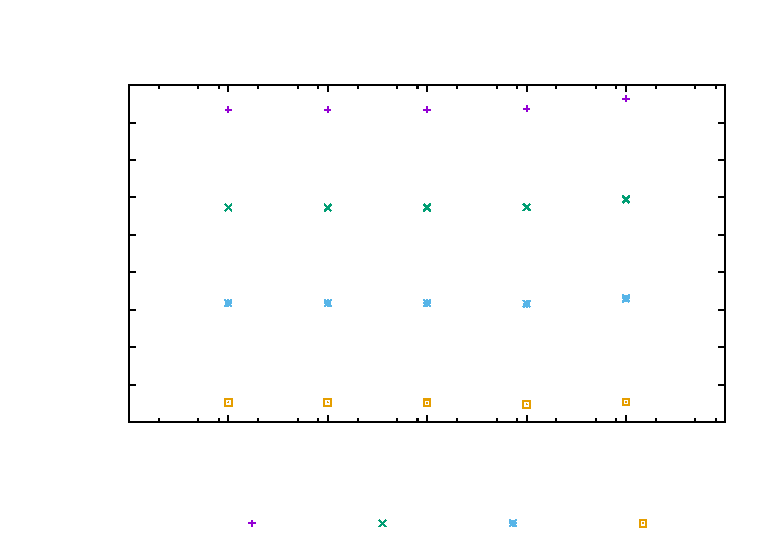
\includegraphics{../../Programming/sinking_bim_write_up/trunk/fin_pos_viscos}}%
    \gplfronttext
  \end{picture}%
\endgroup
}
    \caption{Plots of $z_{\text{eq}}$ versus $\lambda$ for $\Bo = 1$ and different values of $D$. It is seen that there is no dependence on $\lambda$. The same is true for other values of $\Bo$. \label{fig:fin_pos_viscos}}
  \end{figure}

  \begin{figure}
    \resizebox{0.9\textwidth}{!}{\large % GNUPLOT: LaTeX picture with Postscript
\begingroup
  \makeatletter
  \providecommand\color[2][]{%
    \GenericError{(gnuplot) \space\space\space\@spaces}{%
      Package color not loaded in conjunction with
      terminal option `colourtext'%
    }{See the gnuplot documentation for explanation.%
    }{Either use 'blacktext' in gnuplot or load the package
      color.sty in LaTeX.}%
    \renewcommand\color[2][]{}%
  }%
  \providecommand\includegraphics[2][]{%
    \GenericError{(gnuplot) \space\space\space\@spaces}{%
      Package graphicx or graphics not loaded%
    }{See the gnuplot documentation for explanation.%
    }{The gnuplot epslatex terminal needs graphicx.sty or graphics.sty.}%
    \renewcommand\includegraphics[2][]{}%
  }%
  \providecommand\rotatebox[2]{#2}%
  \@ifundefined{ifGPcolor}{%
    \newif\ifGPcolor
    \GPcolorfalse
  }{}%
  \@ifundefined{ifGPblacktext}{%
    \newif\ifGPblacktext
    \GPblacktexttrue
  }{}%
  % define a \g@addto@macro without @ in the name:
  \let\gplgaddtomacro\g@addto@macro
  % define empty templates for all commands taking text:
  \gdef\gplbacktext{}%
  \gdef\gplfronttext{}%
  \makeatother
  \ifGPblacktext
    % no textcolor at all
    \def\colorrgb#1{}%
    \def\colorgray#1{}%
  \else
    % gray or color?
    \ifGPcolor
      \def\colorrgb#1{\color[rgb]{#1}}%
      \def\colorgray#1{\color[gray]{#1}}%
      \expandafter\def\csname LTw\endcsname{\color{white}}%
      \expandafter\def\csname LTb\endcsname{\color{black}}%
      \expandafter\def\csname LTa\endcsname{\color{black}}%
      \expandafter\def\csname LT0\endcsname{\color[rgb]{1,0,0}}%
      \expandafter\def\csname LT1\endcsname{\color[rgb]{0,1,0}}%
      \expandafter\def\csname LT2\endcsname{\color[rgb]{0,0,1}}%
      \expandafter\def\csname LT3\endcsname{\color[rgb]{1,0,1}}%
      \expandafter\def\csname LT4\endcsname{\color[rgb]{0,1,1}}%
      \expandafter\def\csname LT5\endcsname{\color[rgb]{1,1,0}}%
      \expandafter\def\csname LT6\endcsname{\color[rgb]{0,0,0}}%
      \expandafter\def\csname LT7\endcsname{\color[rgb]{1,0.3,0}}%
      \expandafter\def\csname LT8\endcsname{\color[rgb]{0.5,0.5,0.5}}%
    \else
      % gray
      \def\colorrgb#1{\color{black}}%
      \def\colorgray#1{\color[gray]{#1}}%
      \expandafter\def\csname LTw\endcsname{\color{white}}%
      \expandafter\def\csname LTb\endcsname{\color{black}}%
      \expandafter\def\csname LTa\endcsname{\color{black}}%
      \expandafter\def\csname LT0\endcsname{\color{black}}%
      \expandafter\def\csname LT1\endcsname{\color{black}}%
      \expandafter\def\csname LT2\endcsname{\color{black}}%
      \expandafter\def\csname LT3\endcsname{\color{black}}%
      \expandafter\def\csname LT4\endcsname{\color{black}}%
      \expandafter\def\csname LT5\endcsname{\color{black}}%
      \expandafter\def\csname LT6\endcsname{\color{black}}%
      \expandafter\def\csname LT7\endcsname{\color{black}}%
      \expandafter\def\csname LT8\endcsname{\color{black}}%
    \fi
  \fi
    \setlength{\unitlength}{0.0500bp}%
    \ifx\gptboxheight\undefined%
      \newlength{\gptboxheight}%
      \newlength{\gptboxwidth}%
      \newsavebox{\gptboxtext}%
    \fi%
    \setlength{\fboxrule}{0.5pt}%
    \setlength{\fboxsep}{1pt}%
\begin{picture}(7200.00,5040.00)%
    \gplgaddtomacro\gplbacktext{%
      \csname LTb\endcsname%
      \put(946,704){\makebox(0,0)[r]{\strut{}$-1$}}%
      \put(946,1038){\makebox(0,0)[r]{\strut{}$-0.8$}}%
      \put(946,1372){\makebox(0,0)[r]{\strut{}$-0.6$}}%
      \put(946,1706){\makebox(0,0)[r]{\strut{}$-0.4$}}%
      \put(946,2040){\makebox(0,0)[r]{\strut{}$-0.2$}}%
      \put(946,2374){\makebox(0,0)[r]{\strut{}$0$}}%
      \put(946,2709){\makebox(0,0)[r]{\strut{}$0.2$}}%
      \put(946,3043){\makebox(0,0)[r]{\strut{}$0.4$}}%
      \put(946,3377){\makebox(0,0)[r]{\strut{}$0.6$}}%
      \put(946,3711){\makebox(0,0)[r]{\strut{}$0.8$}}%
      \put(946,4045){\makebox(0,0)[r]{\strut{}$1$}}%
      \put(946,4379){\makebox(0,0)[r]{\strut{}$1.2$}}%
      \put(1078,484){\makebox(0,0){\strut{}$0.001$}}%
      \put(1896,484){\makebox(0,0){\strut{}$0.01$}}%
      \put(2714,484){\makebox(0,0){\strut{}$0.1$}}%
      \put(3532,484){\makebox(0,0){\strut{}$1$}}%
      \put(4349,484){\makebox(0,0){\strut{}$10$}}%
      \put(5167,484){\makebox(0,0){\strut{}$100$}}%
      \put(5985,484){\makebox(0,0){\strut{}$1000$}}%
      \put(6803,484){\makebox(0,0){\strut{}$10000$}}%
    }%
    \gplgaddtomacro\gplfronttext{%
      \csname LTb\endcsname%
      \put(176,2541){\rotatebox{-270}{\makebox(0,0){\strut{}$z_{\text{eq}}$}}}%
      \put(3940,154){\makebox(0,0){\strut{}$\Bo$}}%
      \put(3940,4709){\makebox(0,0){\strut{}$\lambda = 1$}}%
      \put(6045,4206){\makebox(0,0){\strut{}$D$}}%
      \csname LTb\endcsname%
      \put(5816,3986){\makebox(0,0)[r]{\strut{}1}}%
      \csname LTb\endcsname%
      \put(5816,3766){\makebox(0,0)[r]{\strut{}1.5}}%
      \csname LTb\endcsname%
      \put(5816,3546){\makebox(0,0)[r]{\strut{}2}}%
      \csname LTb\endcsname%
      \put(5816,3326){\makebox(0,0)[r]{\strut{}2.5}}%
    }%
    \gplbacktext
    \put(0,0){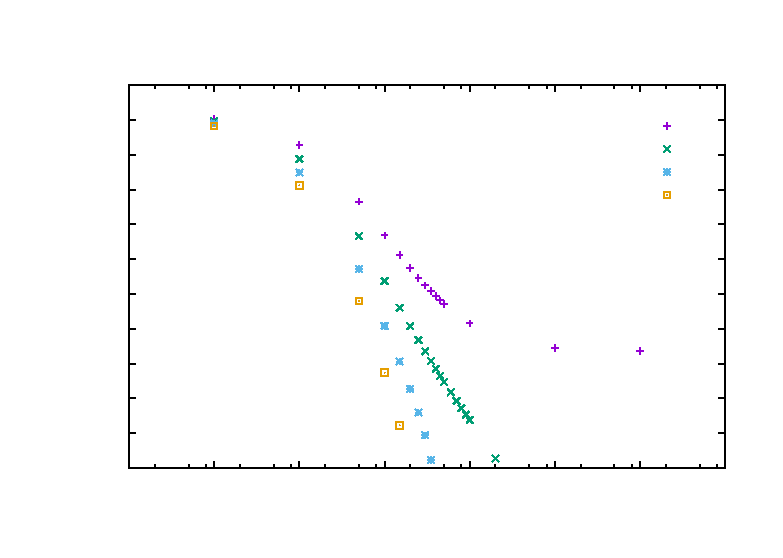
\includegraphics{../../Programming/sinking_bim_write_up/trunk/fin_pos}}%
    \gplfronttext
  \end{picture}%
\endgroup
}
    \caption{Plots of $z_{\text{eq}}$ versus $\Bo$ for $\lambda = 1$ and different values of $D$. As $\Bo \to 0$, $z_{\text{eq}}$ becomes independent of $D$. As $\Bo$ increases, the sphere transitions to sinking and so the plots cannot be continued to higher $\Bo$. \label{fig:fin_pos}}
  \end{figure}

\subsubsection{Entrained Volume}
\label{subsubsec:ent_vol_res}

As described in section~\ref{sec:num_meth}, one of the criteria for the termination of the model is that two separate branches of the interface become closer to each other than the smallest interval length on either the sphere or the interface. In the case, the interface is assumed to snap at this point and the volume of upper phase fluid beneath the point of snapping is defined as the entrained volume $V$. The range of parameters for which the entrained volume was investigated is limited by the termination criteria of the model. For $D < 4$ or $\lambda > 0.03$, most simulations where sinking was observed terminated when the sphere and the interface became too close. For $D = 4$, the same is true for $\Bo <1$ and as $D$ increases, this critical value of $\Bo$ decreases, such that for $D = 1000$ interface snapping was observed down to $\Bo = 0.01$, the smallest value used.

Figure~\ref{fig:mdr_snap} shows the dependence of the entrained volume of $\Bo$ for different values of $D$ and $\lambda$. For $D = 8$ (figure~\ref{fig:mdr=8}), it can be seen that for $\Bo < 1$, $V$ is approximately independent of $\lambda$ and $V \sim \ln\Bo$. For $\Bo > 1$, $V$ becomes independent of $\Bo$ and there is a weak dependence on $\lambda$; the more viscous the upper fluid relative to the lower fluid, the greater the volume of entrained fluid. Increasing $D$ to 50 (figure~\ref{fig:mdr=50}) it can be seen that the viscosity independent linear relationship between $V$ and $\ln\Bo$ is present for $\ln \Bo < -2$ ($\Bo < 0.14$). For larger Bond numbers, $V$ again becomes independent of $\Bo$ although the viscosity dependence is stronger than for $D = 8$. Additionally, for a given $\Bo$ and $\lambda$, $V$ is greater for $D = 50$ than $D = 8$.

These trends are continued to higher values of $D$ (figures~\ref{fig:mdr=100} and~\ref{fig:mdr=1000}). The transitional value of $\Bo$ decreases as $D$ increases; for $D = 1000$ this transitional value is smaller than the smallest $\Bo$ used. Also, as $D$ increases at fixed $\lambda$ and $\Bo$, so does $V$.


    \begin{figure}
      \centering
      \begin{subfigure}[b]{0.45\textwidth}
        \resizebox{\textwidth}{!}{\Large % GNUPLOT: LaTeX picture with Postscript
\begingroup
  \makeatletter
  \providecommand\color[2][]{%
    \GenericError{(gnuplot) \space\space\space\@spaces}{%
      Package color not loaded in conjunction with
      terminal option `colourtext'%
    }{See the gnuplot documentation for explanation.%
    }{Either use 'blacktext' in gnuplot or load the package
      color.sty in LaTeX.}%
    \renewcommand\color[2][]{}%
  }%
  \providecommand\includegraphics[2][]{%
    \GenericError{(gnuplot) \space\space\space\@spaces}{%
      Package graphicx or graphics not loaded%
    }{See the gnuplot documentation for explanation.%
    }{The gnuplot epslatex terminal needs graphicx.sty or graphics.sty.}%
    \renewcommand\includegraphics[2][]{}%
  }%
  \providecommand\rotatebox[2]{#2}%
  \@ifundefined{ifGPcolor}{%
    \newif\ifGPcolor
    \GPcolorfalse
  }{}%
  \@ifundefined{ifGPblacktext}{%
    \newif\ifGPblacktext
    \GPblacktexttrue
  }{}%
  % define a \g@addto@macro without @ in the name:
  \let\gplgaddtomacro\g@addto@macro
  % define empty templates for all commands taking text:
  \gdef\gplbacktext{}%
  \gdef\gplfronttext{}%
  \makeatother
  \ifGPblacktext
    % no textcolor at all
    \def\colorrgb#1{}%
    \def\colorgray#1{}%
  \else
    % gray or color?
    \ifGPcolor
      \def\colorrgb#1{\color[rgb]{#1}}%
      \def\colorgray#1{\color[gray]{#1}}%
      \expandafter\def\csname LTw\endcsname{\color{white}}%
      \expandafter\def\csname LTb\endcsname{\color{black}}%
      \expandafter\def\csname LTa\endcsname{\color{black}}%
      \expandafter\def\csname LT0\endcsname{\color[rgb]{1,0,0}}%
      \expandafter\def\csname LT1\endcsname{\color[rgb]{0,1,0}}%
      \expandafter\def\csname LT2\endcsname{\color[rgb]{0,0,1}}%
      \expandafter\def\csname LT3\endcsname{\color[rgb]{1,0,1}}%
      \expandafter\def\csname LT4\endcsname{\color[rgb]{0,1,1}}%
      \expandafter\def\csname LT5\endcsname{\color[rgb]{1,1,0}}%
      \expandafter\def\csname LT6\endcsname{\color[rgb]{0,0,0}}%
      \expandafter\def\csname LT7\endcsname{\color[rgb]{1,0.3,0}}%
      \expandafter\def\csname LT8\endcsname{\color[rgb]{0.5,0.5,0.5}}%
    \else
      % gray
      \def\colorrgb#1{\color{black}}%
      \def\colorgray#1{\color[gray]{#1}}%
      \expandafter\def\csname LTw\endcsname{\color{white}}%
      \expandafter\def\csname LTb\endcsname{\color{black}}%
      \expandafter\def\csname LTa\endcsname{\color{black}}%
      \expandafter\def\csname LT0\endcsname{\color{black}}%
      \expandafter\def\csname LT1\endcsname{\color{black}}%
      \expandafter\def\csname LT2\endcsname{\color{black}}%
      \expandafter\def\csname LT3\endcsname{\color{black}}%
      \expandafter\def\csname LT4\endcsname{\color{black}}%
      \expandafter\def\csname LT5\endcsname{\color{black}}%
      \expandafter\def\csname LT6\endcsname{\color{black}}%
      \expandafter\def\csname LT7\endcsname{\color{black}}%
      \expandafter\def\csname LT8\endcsname{\color{black}}%
    \fi
  \fi
    \setlength{\unitlength}{0.0500bp}%
    \ifx\gptboxheight\undefined%
      \newlength{\gptboxheight}%
      \newlength{\gptboxwidth}%
      \newsavebox{\gptboxtext}%
    \fi%
    \setlength{\fboxrule}{0.5pt}%
    \setlength{\fboxsep}{1pt}%
\begin{picture}(7200.00,5040.00)%
    \gplgaddtomacro\gplbacktext{%
      \csname LTb\endcsname%
      \put(682,704){\makebox(0,0)[r]{\strut{}$0$}}%
      \put(682,1112){\makebox(0,0)[r]{\strut{}$2$}}%
      \put(682,1521){\makebox(0,0)[r]{\strut{}$4$}}%
      \put(682,1929){\makebox(0,0)[r]{\strut{}$6$}}%
      \put(682,2337){\makebox(0,0)[r]{\strut{}$8$}}%
      \put(682,2746){\makebox(0,0)[r]{\strut{}$10$}}%
      \put(682,3154){\makebox(0,0)[r]{\strut{}$12$}}%
      \put(682,3562){\makebox(0,0)[r]{\strut{}$14$}}%
      \put(682,3971){\makebox(0,0)[r]{\strut{}$16$}}%
      \put(682,4379){\makebox(0,0)[r]{\strut{}$18$}}%
      \put(814,484){\makebox(0,0){\strut{}$-6$}}%
      \put(1670,484){\makebox(0,0){\strut{}$-4$}}%
      \put(2525,484){\makebox(0,0){\strut{}$-2$}}%
      \put(3381,484){\makebox(0,0){\strut{}$0$}}%
      \put(4236,484){\makebox(0,0){\strut{}$2$}}%
      \put(5092,484){\makebox(0,0){\strut{}$4$}}%
      \put(5947,484){\makebox(0,0){\strut{}$6$}}%
      \put(6803,484){\makebox(0,0){\strut{}$8$}}%
    }%
    \gplgaddtomacro\gplfronttext{%
      \csname LTb\endcsname%
      \put(176,2541){\rotatebox{-270}{\makebox(0,0){\strut{}$V$}}}%
      \put(3808,154){\makebox(0,0){\strut{}$\ln\Bo$}}%
      \put(3808,4709){\makebox(0,0){\strut{}$D = 8$}}%
      \put(1703,4151){\makebox(0,0){\strut{}$\lambda$}}%
      \csname LTb\endcsname%
      \put(1606,3931){\makebox(0,0)[r]{\strut{}0.001}}%
      \csname LTb\endcsname%
      \put(1606,3601){\makebox(0,0)[r]{\strut{}0.003}}%
      \csname LTb\endcsname%
      \put(1606,3271){\makebox(0,0)[r]{\strut{}0.005}}%
      \csname LTb\endcsname%
      \put(1606,2941){\makebox(0,0)[r]{\strut{}0.008}}%
      \csname LTb\endcsname%
      \put(1606,2611){\makebox(0,0)[r]{\strut{}0.01}}%
      \csname LTb\endcsname%
      \put(1606,2281){\makebox(0,0)[r]{\strut{}0.03}}%
    }%
    \gplbacktext
    \put(0,0){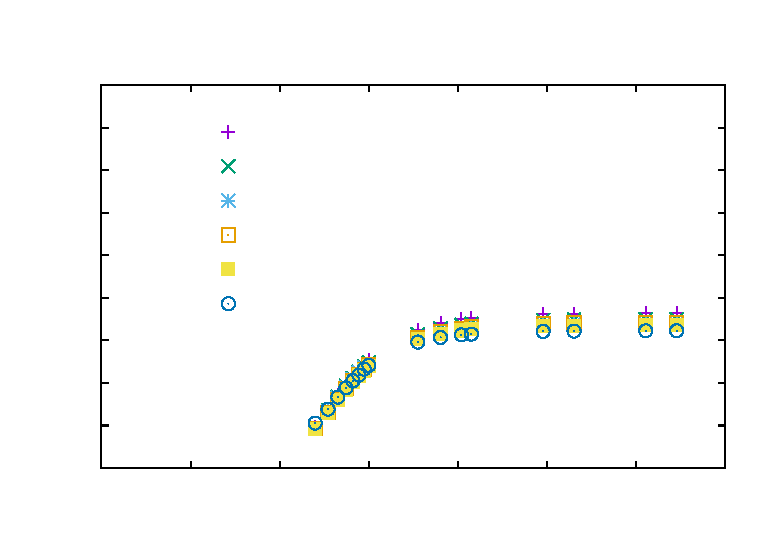
\includegraphics{../../Programming/sinking_bim_write_up/trunk/mdr=8_pub}}%
    \gplfronttext
  \end{picture}%
\endgroup
}
        \caption{}
        \label{fig:mdr=8}
      \end{subfigure}
      ~
      \begin{subfigure}[b]{0.45\textwidth}
        \resizebox{\textwidth}{!}{\Large % GNUPLOT: LaTeX picture with Postscript
\begingroup
  \makeatletter
  \providecommand\color[2][]{%
    \GenericError{(gnuplot) \space\space\space\@spaces}{%
      Package color not loaded in conjunction with
      terminal option `colourtext'%
    }{See the gnuplot documentation for explanation.%
    }{Either use 'blacktext' in gnuplot or load the package
      color.sty in LaTeX.}%
    \renewcommand\color[2][]{}%
  }%
  \providecommand\includegraphics[2][]{%
    \GenericError{(gnuplot) \space\space\space\@spaces}{%
      Package graphicx or graphics not loaded%
    }{See the gnuplot documentation for explanation.%
    }{The gnuplot epslatex terminal needs graphicx.sty or graphics.sty.}%
    \renewcommand\includegraphics[2][]{}%
  }%
  \providecommand\rotatebox[2]{#2}%
  \@ifundefined{ifGPcolor}{%
    \newif\ifGPcolor
    \GPcolorfalse
  }{}%
  \@ifundefined{ifGPblacktext}{%
    \newif\ifGPblacktext
    \GPblacktexttrue
  }{}%
  % define a \g@addto@macro without @ in the name:
  \let\gplgaddtomacro\g@addto@macro
  % define empty templates for all commands taking text:
  \gdef\gplbacktext{}%
  \gdef\gplfronttext{}%
  \makeatother
  \ifGPblacktext
    % no textcolor at all
    \def\colorrgb#1{}%
    \def\colorgray#1{}%
  \else
    % gray or color?
    \ifGPcolor
      \def\colorrgb#1{\color[rgb]{#1}}%
      \def\colorgray#1{\color[gray]{#1}}%
      \expandafter\def\csname LTw\endcsname{\color{white}}%
      \expandafter\def\csname LTb\endcsname{\color{black}}%
      \expandafter\def\csname LTa\endcsname{\color{black}}%
      \expandafter\def\csname LT0\endcsname{\color[rgb]{1,0,0}}%
      \expandafter\def\csname LT1\endcsname{\color[rgb]{0,1,0}}%
      \expandafter\def\csname LT2\endcsname{\color[rgb]{0,0,1}}%
      \expandafter\def\csname LT3\endcsname{\color[rgb]{1,0,1}}%
      \expandafter\def\csname LT4\endcsname{\color[rgb]{0,1,1}}%
      \expandafter\def\csname LT5\endcsname{\color[rgb]{1,1,0}}%
      \expandafter\def\csname LT6\endcsname{\color[rgb]{0,0,0}}%
      \expandafter\def\csname LT7\endcsname{\color[rgb]{1,0.3,0}}%
      \expandafter\def\csname LT8\endcsname{\color[rgb]{0.5,0.5,0.5}}%
    \else
      % gray
      \def\colorrgb#1{\color{black}}%
      \def\colorgray#1{\color[gray]{#1}}%
      \expandafter\def\csname LTw\endcsname{\color{white}}%
      \expandafter\def\csname LTb\endcsname{\color{black}}%
      \expandafter\def\csname LTa\endcsname{\color{black}}%
      \expandafter\def\csname LT0\endcsname{\color{black}}%
      \expandafter\def\csname LT1\endcsname{\color{black}}%
      \expandafter\def\csname LT2\endcsname{\color{black}}%
      \expandafter\def\csname LT3\endcsname{\color{black}}%
      \expandafter\def\csname LT4\endcsname{\color{black}}%
      \expandafter\def\csname LT5\endcsname{\color{black}}%
      \expandafter\def\csname LT6\endcsname{\color{black}}%
      \expandafter\def\csname LT7\endcsname{\color{black}}%
      \expandafter\def\csname LT8\endcsname{\color{black}}%
    \fi
  \fi
    \setlength{\unitlength}{0.0500bp}%
    \ifx\gptboxheight\undefined%
      \newlength{\gptboxheight}%
      \newlength{\gptboxwidth}%
      \newsavebox{\gptboxtext}%
    \fi%
    \setlength{\fboxrule}{0.5pt}%
    \setlength{\fboxsep}{1pt}%
\begin{picture}(7200.00,5040.00)%
    \gplgaddtomacro\gplbacktext{%
      \csname LTb\endcsname%
      \put(682,704){\makebox(0,0)[r]{\strut{}$0$}}%
      \put(682,1112){\makebox(0,0)[r]{\strut{}$2$}}%
      \put(682,1521){\makebox(0,0)[r]{\strut{}$4$}}%
      \put(682,1929){\makebox(0,0)[r]{\strut{}$6$}}%
      \put(682,2337){\makebox(0,0)[r]{\strut{}$8$}}%
      \put(682,2746){\makebox(0,0)[r]{\strut{}$10$}}%
      \put(682,3154){\makebox(0,0)[r]{\strut{}$12$}}%
      \put(682,3562){\makebox(0,0)[r]{\strut{}$14$}}%
      \put(682,3971){\makebox(0,0)[r]{\strut{}$16$}}%
      \put(682,4379){\makebox(0,0)[r]{\strut{}$18$}}%
      \put(814,484){\makebox(0,0){\strut{}$-6$}}%
      \put(1670,484){\makebox(0,0){\strut{}$-4$}}%
      \put(2525,484){\makebox(0,0){\strut{}$-2$}}%
      \put(3381,484){\makebox(0,0){\strut{}$0$}}%
      \put(4236,484){\makebox(0,0){\strut{}$2$}}%
      \put(5092,484){\makebox(0,0){\strut{}$4$}}%
      \put(5947,484){\makebox(0,0){\strut{}$6$}}%
      \put(6803,484){\makebox(0,0){\strut{}$8$}}%
    }%
    \gplgaddtomacro\gplfronttext{%
      \csname LTb\endcsname%
      \put(176,2541){\rotatebox{-270}{\makebox(0,0){\strut{}$V$}}}%
      \put(3808,154){\makebox(0,0){\strut{}$\ln\Bo$}}%
      \put(3808,4709){\makebox(0,0){\strut{}$D = 50$}}%
    }%
    \gplbacktext
    \put(0,0){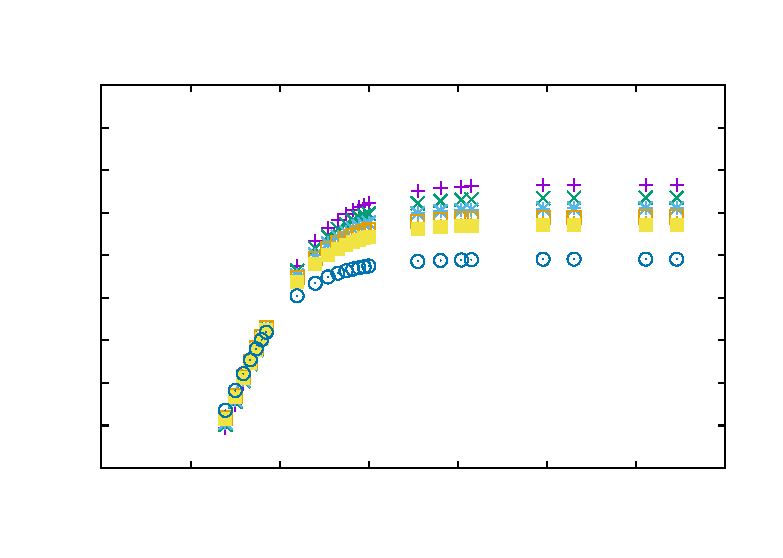
\includegraphics{mdr=50_pub}}%
    \gplfronttext
  \end{picture}%
\endgroup
}
        \caption{}
        \label{fig:mdr=50}
      \end{subfigure}
      
      \begin{subfigure}[b]{0.45\textwidth}
        \resizebox{\textwidth}{!}{\Large % GNUPLOT: LaTeX picture with Postscript
\begingroup
  \makeatletter
  \providecommand\color[2][]{%
    \GenericError{(gnuplot) \space\space\space\@spaces}{%
      Package color not loaded in conjunction with
      terminal option `colourtext'%
    }{See the gnuplot documentation for explanation.%
    }{Either use 'blacktext' in gnuplot or load the package
      color.sty in LaTeX.}%
    \renewcommand\color[2][]{}%
  }%
  \providecommand\includegraphics[2][]{%
    \GenericError{(gnuplot) \space\space\space\@spaces}{%
      Package graphicx or graphics not loaded%
    }{See the gnuplot documentation for explanation.%
    }{The gnuplot epslatex terminal needs graphicx.sty or graphics.sty.}%
    \renewcommand\includegraphics[2][]{}%
  }%
  \providecommand\rotatebox[2]{#2}%
  \@ifundefined{ifGPcolor}{%
    \newif\ifGPcolor
    \GPcolorfalse
  }{}%
  \@ifundefined{ifGPblacktext}{%
    \newif\ifGPblacktext
    \GPblacktexttrue
  }{}%
  % define a \g@addto@macro without @ in the name:
  \let\gplgaddtomacro\g@addto@macro
  % define empty templates for all commands taking text:
  \gdef\gplbacktext{}%
  \gdef\gplfronttext{}%
  \makeatother
  \ifGPblacktext
    % no textcolor at all
    \def\colorrgb#1{}%
    \def\colorgray#1{}%
  \else
    % gray or color?
    \ifGPcolor
      \def\colorrgb#1{\color[rgb]{#1}}%
      \def\colorgray#1{\color[gray]{#1}}%
      \expandafter\def\csname LTw\endcsname{\color{white}}%
      \expandafter\def\csname LTb\endcsname{\color{black}}%
      \expandafter\def\csname LTa\endcsname{\color{black}}%
      \expandafter\def\csname LT0\endcsname{\color[rgb]{1,0,0}}%
      \expandafter\def\csname LT1\endcsname{\color[rgb]{0,1,0}}%
      \expandafter\def\csname LT2\endcsname{\color[rgb]{0,0,1}}%
      \expandafter\def\csname LT3\endcsname{\color[rgb]{1,0,1}}%
      \expandafter\def\csname LT4\endcsname{\color[rgb]{0,1,1}}%
      \expandafter\def\csname LT5\endcsname{\color[rgb]{1,1,0}}%
      \expandafter\def\csname LT6\endcsname{\color[rgb]{0,0,0}}%
      \expandafter\def\csname LT7\endcsname{\color[rgb]{1,0.3,0}}%
      \expandafter\def\csname LT8\endcsname{\color[rgb]{0.5,0.5,0.5}}%
    \else
      % gray
      \def\colorrgb#1{\color{black}}%
      \def\colorgray#1{\color[gray]{#1}}%
      \expandafter\def\csname LTw\endcsname{\color{white}}%
      \expandafter\def\csname LTb\endcsname{\color{black}}%
      \expandafter\def\csname LTa\endcsname{\color{black}}%
      \expandafter\def\csname LT0\endcsname{\color{black}}%
      \expandafter\def\csname LT1\endcsname{\color{black}}%
      \expandafter\def\csname LT2\endcsname{\color{black}}%
      \expandafter\def\csname LT3\endcsname{\color{black}}%
      \expandafter\def\csname LT4\endcsname{\color{black}}%
      \expandafter\def\csname LT5\endcsname{\color{black}}%
      \expandafter\def\csname LT6\endcsname{\color{black}}%
      \expandafter\def\csname LT7\endcsname{\color{black}}%
      \expandafter\def\csname LT8\endcsname{\color{black}}%
    \fi
  \fi
    \setlength{\unitlength}{0.0500bp}%
    \ifx\gptboxheight\undefined%
      \newlength{\gptboxheight}%
      \newlength{\gptboxwidth}%
      \newsavebox{\gptboxtext}%
    \fi%
    \setlength{\fboxrule}{0.5pt}%
    \setlength{\fboxsep}{1pt}%
\begin{picture}(7200.00,5040.00)%
    \gplgaddtomacro\gplbacktext{%
      \csname LTb\endcsname%
      \put(682,704){\makebox(0,0)[r]{\strut{}$0$}}%
      \put(682,1112){\makebox(0,0)[r]{\strut{}$2$}}%
      \put(682,1521){\makebox(0,0)[r]{\strut{}$4$}}%
      \put(682,1929){\makebox(0,0)[r]{\strut{}$6$}}%
      \put(682,2337){\makebox(0,0)[r]{\strut{}$8$}}%
      \put(682,2746){\makebox(0,0)[r]{\strut{}$10$}}%
      \put(682,3154){\makebox(0,0)[r]{\strut{}$12$}}%
      \put(682,3562){\makebox(0,0)[r]{\strut{}$14$}}%
      \put(682,3971){\makebox(0,0)[r]{\strut{}$16$}}%
      \put(682,4379){\makebox(0,0)[r]{\strut{}$18$}}%
      \put(814,484){\makebox(0,0){\strut{}$-6$}}%
      \put(1670,484){\makebox(0,0){\strut{}$-4$}}%
      \put(2525,484){\makebox(0,0){\strut{}$-2$}}%
      \put(3381,484){\makebox(0,0){\strut{}$0$}}%
      \put(4236,484){\makebox(0,0){\strut{}$2$}}%
      \put(5092,484){\makebox(0,0){\strut{}$4$}}%
      \put(5947,484){\makebox(0,0){\strut{}$6$}}%
      \put(6803,484){\makebox(0,0){\strut{}$8$}}%
    }%
    \gplgaddtomacro\gplfronttext{%
      \csname LTb\endcsname%
      \put(176,2541){\rotatebox{-270}{\makebox(0,0){\strut{}$V$}}}%
      \put(3808,154){\makebox(0,0){\strut{}$\ln\Bo$}}%
      \put(3808,4709){\makebox(0,0){\strut{}$D = 100$}}%
    }%
    \gplbacktext
    \put(0,0){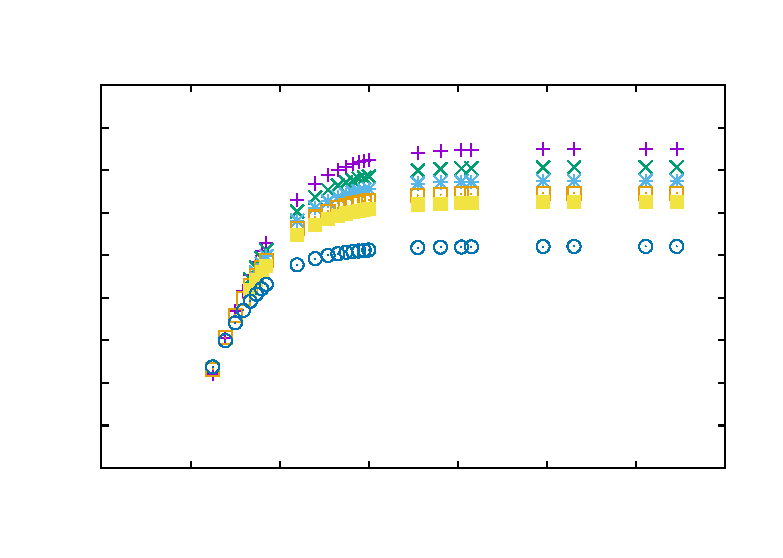
\includegraphics{mdr=100_pub}}%
    \gplfronttext
  \end{picture}%
\endgroup
}
        \caption{}
        \label{fig:mdr=100}
      \end{subfigure}
      ~
      \begin{subfigure}[b]{0.45\textwidth}
        \resizebox{\textwidth}{!}{\Large % GNUPLOT: LaTeX picture with Postscript
\begingroup
  \makeatletter
  \providecommand\color[2][]{%
    \GenericError{(gnuplot) \space\space\space\@spaces}{%
      Package color not loaded in conjunction with
      terminal option `colourtext'%
    }{See the gnuplot documentation for explanation.%
    }{Either use 'blacktext' in gnuplot or load the package
      color.sty in LaTeX.}%
    \renewcommand\color[2][]{}%
  }%
  \providecommand\includegraphics[2][]{%
    \GenericError{(gnuplot) \space\space\space\@spaces}{%
      Package graphicx or graphics not loaded%
    }{See the gnuplot documentation for explanation.%
    }{The gnuplot epslatex terminal needs graphicx.sty or graphics.sty.}%
    \renewcommand\includegraphics[2][]{}%
  }%
  \providecommand\rotatebox[2]{#2}%
  \@ifundefined{ifGPcolor}{%
    \newif\ifGPcolor
    \GPcolorfalse
  }{}%
  \@ifundefined{ifGPblacktext}{%
    \newif\ifGPblacktext
    \GPblacktexttrue
  }{}%
  % define a \g@addto@macro without @ in the name:
  \let\gplgaddtomacro\g@addto@macro
  % define empty templates for all commands taking text:
  \gdef\gplbacktext{}%
  \gdef\gplfronttext{}%
  \makeatother
  \ifGPblacktext
    % no textcolor at all
    \def\colorrgb#1{}%
    \def\colorgray#1{}%
  \else
    % gray or color?
    \ifGPcolor
      \def\colorrgb#1{\color[rgb]{#1}}%
      \def\colorgray#1{\color[gray]{#1}}%
      \expandafter\def\csname LTw\endcsname{\color{white}}%
      \expandafter\def\csname LTb\endcsname{\color{black}}%
      \expandafter\def\csname LTa\endcsname{\color{black}}%
      \expandafter\def\csname LT0\endcsname{\color[rgb]{1,0,0}}%
      \expandafter\def\csname LT1\endcsname{\color[rgb]{0,1,0}}%
      \expandafter\def\csname LT2\endcsname{\color[rgb]{0,0,1}}%
      \expandafter\def\csname LT3\endcsname{\color[rgb]{1,0,1}}%
      \expandafter\def\csname LT4\endcsname{\color[rgb]{0,1,1}}%
      \expandafter\def\csname LT5\endcsname{\color[rgb]{1,1,0}}%
      \expandafter\def\csname LT6\endcsname{\color[rgb]{0,0,0}}%
      \expandafter\def\csname LT7\endcsname{\color[rgb]{1,0.3,0}}%
      \expandafter\def\csname LT8\endcsname{\color[rgb]{0.5,0.5,0.5}}%
    \else
      % gray
      \def\colorrgb#1{\color{black}}%
      \def\colorgray#1{\color[gray]{#1}}%
      \expandafter\def\csname LTw\endcsname{\color{white}}%
      \expandafter\def\csname LTb\endcsname{\color{black}}%
      \expandafter\def\csname LTa\endcsname{\color{black}}%
      \expandafter\def\csname LT0\endcsname{\color{black}}%
      \expandafter\def\csname LT1\endcsname{\color{black}}%
      \expandafter\def\csname LT2\endcsname{\color{black}}%
      \expandafter\def\csname LT3\endcsname{\color{black}}%
      \expandafter\def\csname LT4\endcsname{\color{black}}%
      \expandafter\def\csname LT5\endcsname{\color{black}}%
      \expandafter\def\csname LT6\endcsname{\color{black}}%
      \expandafter\def\csname LT7\endcsname{\color{black}}%
      \expandafter\def\csname LT8\endcsname{\color{black}}%
    \fi
  \fi
    \setlength{\unitlength}{0.0500bp}%
    \ifx\gptboxheight\undefined%
      \newlength{\gptboxheight}%
      \newlength{\gptboxwidth}%
      \newsavebox{\gptboxtext}%
    \fi%
    \setlength{\fboxrule}{0.5pt}%
    \setlength{\fboxsep}{1pt}%
\begin{picture}(7200.00,5040.00)%
    \gplgaddtomacro\gplbacktext{%
      \csname LTb\endcsname%
      \put(682,704){\makebox(0,0)[r]{\strut{}$0$}}%
      \put(682,1112){\makebox(0,0)[r]{\strut{}$2$}}%
      \put(682,1521){\makebox(0,0)[r]{\strut{}$4$}}%
      \put(682,1929){\makebox(0,0)[r]{\strut{}$6$}}%
      \put(682,2337){\makebox(0,0)[r]{\strut{}$8$}}%
      \put(682,2746){\makebox(0,0)[r]{\strut{}$10$}}%
      \put(682,3154){\makebox(0,0)[r]{\strut{}$12$}}%
      \put(682,3562){\makebox(0,0)[r]{\strut{}$14$}}%
      \put(682,3971){\makebox(0,0)[r]{\strut{}$16$}}%
      \put(682,4379){\makebox(0,0)[r]{\strut{}$18$}}%
      \put(814,484){\makebox(0,0){\strut{}$-6$}}%
      \put(1670,484){\makebox(0,0){\strut{}$-4$}}%
      \put(2525,484){\makebox(0,0){\strut{}$-2$}}%
      \put(3381,484){\makebox(0,0){\strut{}$0$}}%
      \put(4236,484){\makebox(0,0){\strut{}$2$}}%
      \put(5092,484){\makebox(0,0){\strut{}$4$}}%
      \put(5947,484){\makebox(0,0){\strut{}$6$}}%
      \put(6803,484){\makebox(0,0){\strut{}$8$}}%
    }%
    \gplgaddtomacro\gplfronttext{%
      \csname LTb\endcsname%
      \put(176,2541){\rotatebox{-270}{\makebox(0,0){\strut{}$V$}}}%
      \put(3808,154){\makebox(0,0){\strut{}$\ln\Bo$}}%
      \put(3808,4709){\makebox(0,0){\strut{}$D = 1000$}}%
    }%
    \gplbacktext
    \put(0,0){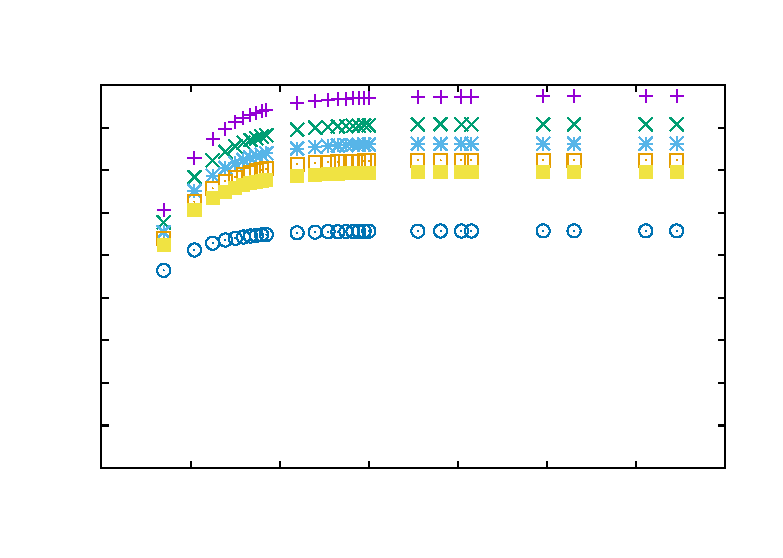
\includegraphics{../../Programming/sinking_bim_write_up/trunk/mdr=1000_pub}}%
    \gplfronttext
  \end{picture}%
\endgroup
}
        \caption{}
        \label{fig:mdr=1000}
      \end{subfigure}
      \caption{Dependence of entrained volume $V$ on $\Bo$ for different $\lambda$ for a) $D = 8$, b) $D = 50$, c) $D = 100$ and d) $D = 1000$. At small $\Bo$ there seems to be a linear relationship between $V$ and $\ln\Bo$ but as $\Bo$ increases, $V$ becomes independent of $\Bo$. }\label{fig:mdr_snap}
    \end{figure}

Figure~\ref{fig:viscos_snap} shows the same data as in figure~\ref{fig:mdr_snap} but with curves with different values of $D$ shown on the same plot with a fixed value of $\lambda$. All of the previously described features can be observed including the two regimes: $V \sim \ln\Bo$ and $V \neq V(\Bo)$, and the increase in $V$ with increasing $D$ and decreasing $\lambda$.

    \begin{figure}
      \centering
      \begin{subfigure}[b]{0.45\textwidth}
        \resizebox{\textwidth}{!}{\Large % GNUPLOT: LaTeX picture with Postscript
\begingroup
  \makeatletter
  \providecommand\color[2][]{%
    \GenericError{(gnuplot) \space\space\space\@spaces}{%
      Package color not loaded in conjunction with
      terminal option `colourtext'%
    }{See the gnuplot documentation for explanation.%
    }{Either use 'blacktext' in gnuplot or load the package
      color.sty in LaTeX.}%
    \renewcommand\color[2][]{}%
  }%
  \providecommand\includegraphics[2][]{%
    \GenericError{(gnuplot) \space\space\space\@spaces}{%
      Package graphicx or graphics not loaded%
    }{See the gnuplot documentation for explanation.%
    }{The gnuplot epslatex terminal needs graphicx.sty or graphics.sty.}%
    \renewcommand\includegraphics[2][]{}%
  }%
  \providecommand\rotatebox[2]{#2}%
  \@ifundefined{ifGPcolor}{%
    \newif\ifGPcolor
    \GPcolorfalse
  }{}%
  \@ifundefined{ifGPblacktext}{%
    \newif\ifGPblacktext
    \GPblacktexttrue
  }{}%
  % define a \g@addto@macro without @ in the name:
  \let\gplgaddtomacro\g@addto@macro
  % define empty templates for all commands taking text:
  \gdef\gplbacktext{}%
  \gdef\gplfronttext{}%
  \makeatother
  \ifGPblacktext
    % no textcolor at all
    \def\colorrgb#1{}%
    \def\colorgray#1{}%
  \else
    % gray or color?
    \ifGPcolor
      \def\colorrgb#1{\color[rgb]{#1}}%
      \def\colorgray#1{\color[gray]{#1}}%
      \expandafter\def\csname LTw\endcsname{\color{white}}%
      \expandafter\def\csname LTb\endcsname{\color{black}}%
      \expandafter\def\csname LTa\endcsname{\color{black}}%
      \expandafter\def\csname LT0\endcsname{\color[rgb]{1,0,0}}%
      \expandafter\def\csname LT1\endcsname{\color[rgb]{0,1,0}}%
      \expandafter\def\csname LT2\endcsname{\color[rgb]{0,0,1}}%
      \expandafter\def\csname LT3\endcsname{\color[rgb]{1,0,1}}%
      \expandafter\def\csname LT4\endcsname{\color[rgb]{0,1,1}}%
      \expandafter\def\csname LT5\endcsname{\color[rgb]{1,1,0}}%
      \expandafter\def\csname LT6\endcsname{\color[rgb]{0,0,0}}%
      \expandafter\def\csname LT7\endcsname{\color[rgb]{1,0.3,0}}%
      \expandafter\def\csname LT8\endcsname{\color[rgb]{0.5,0.5,0.5}}%
    \else
      % gray
      \def\colorrgb#1{\color{black}}%
      \def\colorgray#1{\color[gray]{#1}}%
      \expandafter\def\csname LTw\endcsname{\color{white}}%
      \expandafter\def\csname LTb\endcsname{\color{black}}%
      \expandafter\def\csname LTa\endcsname{\color{black}}%
      \expandafter\def\csname LT0\endcsname{\color{black}}%
      \expandafter\def\csname LT1\endcsname{\color{black}}%
      \expandafter\def\csname LT2\endcsname{\color{black}}%
      \expandafter\def\csname LT3\endcsname{\color{black}}%
      \expandafter\def\csname LT4\endcsname{\color{black}}%
      \expandafter\def\csname LT5\endcsname{\color{black}}%
      \expandafter\def\csname LT6\endcsname{\color{black}}%
      \expandafter\def\csname LT7\endcsname{\color{black}}%
      \expandafter\def\csname LT8\endcsname{\color{black}}%
    \fi
  \fi
    \setlength{\unitlength}{0.0500bp}%
    \ifx\gptboxheight\undefined%
      \newlength{\gptboxheight}%
      \newlength{\gptboxwidth}%
      \newsavebox{\gptboxtext}%
    \fi%
    \setlength{\fboxrule}{0.5pt}%
    \setlength{\fboxsep}{1pt}%
\begin{picture}(7200.00,5040.00)%
    \gplgaddtomacro\gplbacktext{%
      \csname LTb\endcsname%
      \put(682,704){\makebox(0,0)[r]{\strut{}$0$}}%
      \put(682,1112){\makebox(0,0)[r]{\strut{}$2$}}%
      \put(682,1521){\makebox(0,0)[r]{\strut{}$4$}}%
      \put(682,1929){\makebox(0,0)[r]{\strut{}$6$}}%
      \put(682,2337){\makebox(0,0)[r]{\strut{}$8$}}%
      \put(682,2746){\makebox(0,0)[r]{\strut{}$10$}}%
      \put(682,3154){\makebox(0,0)[r]{\strut{}$12$}}%
      \put(682,3562){\makebox(0,0)[r]{\strut{}$14$}}%
      \put(682,3971){\makebox(0,0)[r]{\strut{}$16$}}%
      \put(682,4379){\makebox(0,0)[r]{\strut{}$18$}}%
      \put(814,484){\makebox(0,0){\strut{}$-6$}}%
      \put(1670,484){\makebox(0,0){\strut{}$-4$}}%
      \put(2525,484){\makebox(0,0){\strut{}$-2$}}%
      \put(3381,484){\makebox(0,0){\strut{}$0$}}%
      \put(4236,484){\makebox(0,0){\strut{}$2$}}%
      \put(5092,484){\makebox(0,0){\strut{}$4$}}%
      \put(5947,484){\makebox(0,0){\strut{}$6$}}%
      \put(6803,484){\makebox(0,0){\strut{}$8$}}%
    }%
    \gplgaddtomacro\gplfronttext{%
      \csname LTb\endcsname%
      \put(176,2541){\rotatebox{-270}{\makebox(0,0){\strut{}$V$}}}%
      \put(3808,154){\makebox(0,0){\strut{}$\ln\Bo$}}%
      \put(3808,4709){\makebox(0,0){\strut{}$\lambda = 0.001$}}%
    }%
    \gplbacktext
    \put(0,0){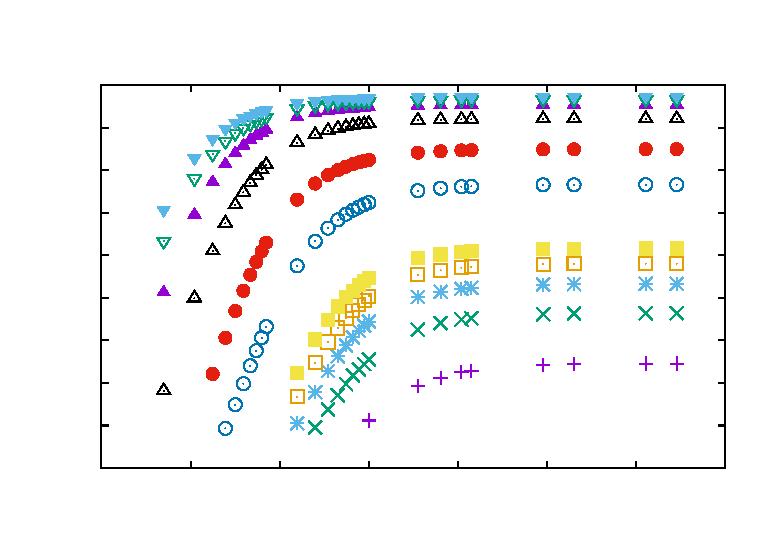
\includegraphics{viscos_rat=001_pub}}%
    \gplfronttext
  \end{picture}%
\endgroup
}
        \caption{}
        \label{fig:viscos_rat=0.001}
      \end{subfigure}
      ~
      \begin{subfigure}[b]{0.45\textwidth}
        \resizebox{\textwidth}{!}{\Large % GNUPLOT: LaTeX picture with Postscript
\begingroup
  \makeatletter
  \providecommand\color[2][]{%
    \GenericError{(gnuplot) \space\space\space\@spaces}{%
      Package color not loaded in conjunction with
      terminal option `colourtext'%
    }{See the gnuplot documentation for explanation.%
    }{Either use 'blacktext' in gnuplot or load the package
      color.sty in LaTeX.}%
    \renewcommand\color[2][]{}%
  }%
  \providecommand\includegraphics[2][]{%
    \GenericError{(gnuplot) \space\space\space\@spaces}{%
      Package graphicx or graphics not loaded%
    }{See the gnuplot documentation for explanation.%
    }{The gnuplot epslatex terminal needs graphicx.sty or graphics.sty.}%
    \renewcommand\includegraphics[2][]{}%
  }%
  \providecommand\rotatebox[2]{#2}%
  \@ifundefined{ifGPcolor}{%
    \newif\ifGPcolor
    \GPcolorfalse
  }{}%
  \@ifundefined{ifGPblacktext}{%
    \newif\ifGPblacktext
    \GPblacktexttrue
  }{}%
  % define a \g@addto@macro without @ in the name:
  \let\gplgaddtomacro\g@addto@macro
  % define empty templates for all commands taking text:
  \gdef\gplbacktext{}%
  \gdef\gplfronttext{}%
  \makeatother
  \ifGPblacktext
    % no textcolor at all
    \def\colorrgb#1{}%
    \def\colorgray#1{}%
  \else
    % gray or color?
    \ifGPcolor
      \def\colorrgb#1{\color[rgb]{#1}}%
      \def\colorgray#1{\color[gray]{#1}}%
      \expandafter\def\csname LTw\endcsname{\color{white}}%
      \expandafter\def\csname LTb\endcsname{\color{black}}%
      \expandafter\def\csname LTa\endcsname{\color{black}}%
      \expandafter\def\csname LT0\endcsname{\color[rgb]{1,0,0}}%
      \expandafter\def\csname LT1\endcsname{\color[rgb]{0,1,0}}%
      \expandafter\def\csname LT2\endcsname{\color[rgb]{0,0,1}}%
      \expandafter\def\csname LT3\endcsname{\color[rgb]{1,0,1}}%
      \expandafter\def\csname LT4\endcsname{\color[rgb]{0,1,1}}%
      \expandafter\def\csname LT5\endcsname{\color[rgb]{1,1,0}}%
      \expandafter\def\csname LT6\endcsname{\color[rgb]{0,0,0}}%
      \expandafter\def\csname LT7\endcsname{\color[rgb]{1,0.3,0}}%
      \expandafter\def\csname LT8\endcsname{\color[rgb]{0.5,0.5,0.5}}%
    \else
      % gray
      \def\colorrgb#1{\color{black}}%
      \def\colorgray#1{\color[gray]{#1}}%
      \expandafter\def\csname LTw\endcsname{\color{white}}%
      \expandafter\def\csname LTb\endcsname{\color{black}}%
      \expandafter\def\csname LTa\endcsname{\color{black}}%
      \expandafter\def\csname LT0\endcsname{\color{black}}%
      \expandafter\def\csname LT1\endcsname{\color{black}}%
      \expandafter\def\csname LT2\endcsname{\color{black}}%
      \expandafter\def\csname LT3\endcsname{\color{black}}%
      \expandafter\def\csname LT4\endcsname{\color{black}}%
      \expandafter\def\csname LT5\endcsname{\color{black}}%
      \expandafter\def\csname LT6\endcsname{\color{black}}%
      \expandafter\def\csname LT7\endcsname{\color{black}}%
      \expandafter\def\csname LT8\endcsname{\color{black}}%
    \fi
  \fi
    \setlength{\unitlength}{0.0500bp}%
    \ifx\gptboxheight\undefined%
      \newlength{\gptboxheight}%
      \newlength{\gptboxwidth}%
      \newsavebox{\gptboxtext}%
    \fi%
    \setlength{\fboxrule}{0.5pt}%
    \setlength{\fboxsep}{1pt}%
\begin{picture}(7200.00,5040.00)%
    \gplgaddtomacro\gplbacktext{%
      \csname LTb\endcsname%
      \put(682,704){\makebox(0,0)[r]{\strut{}$0$}}%
      \put(682,1112){\makebox(0,0)[r]{\strut{}$2$}}%
      \put(682,1521){\makebox(0,0)[r]{\strut{}$4$}}%
      \put(682,1929){\makebox(0,0)[r]{\strut{}$6$}}%
      \put(682,2337){\makebox(0,0)[r]{\strut{}$8$}}%
      \put(682,2746){\makebox(0,0)[r]{\strut{}$10$}}%
      \put(682,3154){\makebox(0,0)[r]{\strut{}$12$}}%
      \put(682,3562){\makebox(0,0)[r]{\strut{}$14$}}%
      \put(682,3971){\makebox(0,0)[r]{\strut{}$16$}}%
      \put(682,4379){\makebox(0,0)[r]{\strut{}$18$}}%
      \put(814,484){\makebox(0,0){\strut{}$-6$}}%
      \put(1670,484){\makebox(0,0){\strut{}$-4$}}%
      \put(2525,484){\makebox(0,0){\strut{}$-2$}}%
      \put(3381,484){\makebox(0,0){\strut{}$0$}}%
      \put(4236,484){\makebox(0,0){\strut{}$2$}}%
      \put(5092,484){\makebox(0,0){\strut{}$4$}}%
      \put(5947,484){\makebox(0,0){\strut{}$6$}}%
      \put(6803,484){\makebox(0,0){\strut{}$8$}}%
    }%
    \gplgaddtomacro\gplfronttext{%
      \csname LTb\endcsname%
      \put(176,2541){\rotatebox{-270}{\makebox(0,0){\strut{}$V$}}}%
      \put(3808,154){\makebox(0,0){\strut{}$\ln\Bo$}}%
      \put(3808,4709){\makebox(0,0){\strut{}$\lambda = 0.005$}}%
    }%
    \gplbacktext
    \put(0,0){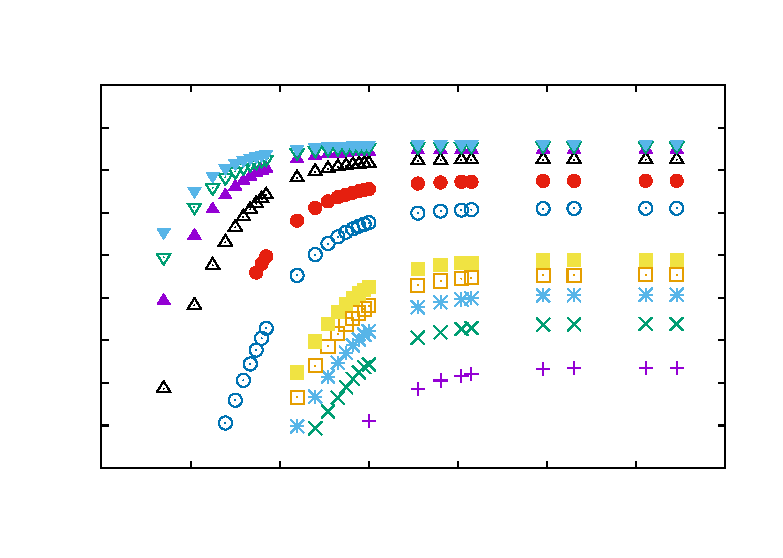
\includegraphics{viscos_rat=005_pub}}%
    \gplfronttext
  \end{picture}%
\endgroup
}
        \caption{}
        \label{fig:viscos_rat=0.005}
      \end{subfigure}
      
      \begin{subfigure}[b]{0.45\textwidth}
        \resizebox{\textwidth}{!}{\Large % GNUPLOT: LaTeX picture with Postscript
\begingroup
  \makeatletter
  \providecommand\color[2][]{%
    \GenericError{(gnuplot) \space\space\space\@spaces}{%
      Package color not loaded in conjunction with
      terminal option `colourtext'%
    }{See the gnuplot documentation for explanation.%
    }{Either use 'blacktext' in gnuplot or load the package
      color.sty in LaTeX.}%
    \renewcommand\color[2][]{}%
  }%
  \providecommand\includegraphics[2][]{%
    \GenericError{(gnuplot) \space\space\space\@spaces}{%
      Package graphicx or graphics not loaded%
    }{See the gnuplot documentation for explanation.%
    }{The gnuplot epslatex terminal needs graphicx.sty or graphics.sty.}%
    \renewcommand\includegraphics[2][]{}%
  }%
  \providecommand\rotatebox[2]{#2}%
  \@ifundefined{ifGPcolor}{%
    \newif\ifGPcolor
    \GPcolorfalse
  }{}%
  \@ifundefined{ifGPblacktext}{%
    \newif\ifGPblacktext
    \GPblacktexttrue
  }{}%
  % define a \g@addto@macro without @ in the name:
  \let\gplgaddtomacro\g@addto@macro
  % define empty templates for all commands taking text:
  \gdef\gplbacktext{}%
  \gdef\gplfronttext{}%
  \makeatother
  \ifGPblacktext
    % no textcolor at all
    \def\colorrgb#1{}%
    \def\colorgray#1{}%
  \else
    % gray or color?
    \ifGPcolor
      \def\colorrgb#1{\color[rgb]{#1}}%
      \def\colorgray#1{\color[gray]{#1}}%
      \expandafter\def\csname LTw\endcsname{\color{white}}%
      \expandafter\def\csname LTb\endcsname{\color{black}}%
      \expandafter\def\csname LTa\endcsname{\color{black}}%
      \expandafter\def\csname LT0\endcsname{\color[rgb]{1,0,0}}%
      \expandafter\def\csname LT1\endcsname{\color[rgb]{0,1,0}}%
      \expandafter\def\csname LT2\endcsname{\color[rgb]{0,0,1}}%
      \expandafter\def\csname LT3\endcsname{\color[rgb]{1,0,1}}%
      \expandafter\def\csname LT4\endcsname{\color[rgb]{0,1,1}}%
      \expandafter\def\csname LT5\endcsname{\color[rgb]{1,1,0}}%
      \expandafter\def\csname LT6\endcsname{\color[rgb]{0,0,0}}%
      \expandafter\def\csname LT7\endcsname{\color[rgb]{1,0.3,0}}%
      \expandafter\def\csname LT8\endcsname{\color[rgb]{0.5,0.5,0.5}}%
    \else
      % gray
      \def\colorrgb#1{\color{black}}%
      \def\colorgray#1{\color[gray]{#1}}%
      \expandafter\def\csname LTw\endcsname{\color{white}}%
      \expandafter\def\csname LTb\endcsname{\color{black}}%
      \expandafter\def\csname LTa\endcsname{\color{black}}%
      \expandafter\def\csname LT0\endcsname{\color{black}}%
      \expandafter\def\csname LT1\endcsname{\color{black}}%
      \expandafter\def\csname LT2\endcsname{\color{black}}%
      \expandafter\def\csname LT3\endcsname{\color{black}}%
      \expandafter\def\csname LT4\endcsname{\color{black}}%
      \expandafter\def\csname LT5\endcsname{\color{black}}%
      \expandafter\def\csname LT6\endcsname{\color{black}}%
      \expandafter\def\csname LT7\endcsname{\color{black}}%
      \expandafter\def\csname LT8\endcsname{\color{black}}%
    \fi
  \fi
    \setlength{\unitlength}{0.0500bp}%
    \ifx\gptboxheight\undefined%
      \newlength{\gptboxheight}%
      \newlength{\gptboxwidth}%
      \newsavebox{\gptboxtext}%
    \fi%
    \setlength{\fboxrule}{0.5pt}%
    \setlength{\fboxsep}{1pt}%
\begin{picture}(7200.00,5040.00)%
    \gplgaddtomacro\gplbacktext{%
      \csname LTb\endcsname%
      \put(682,704){\makebox(0,0)[r]{\strut{}$0$}}%
      \put(682,1112){\makebox(0,0)[r]{\strut{}$2$}}%
      \put(682,1521){\makebox(0,0)[r]{\strut{}$4$}}%
      \put(682,1929){\makebox(0,0)[r]{\strut{}$6$}}%
      \put(682,2337){\makebox(0,0)[r]{\strut{}$8$}}%
      \put(682,2746){\makebox(0,0)[r]{\strut{}$10$}}%
      \put(682,3154){\makebox(0,0)[r]{\strut{}$12$}}%
      \put(682,3562){\makebox(0,0)[r]{\strut{}$14$}}%
      \put(682,3971){\makebox(0,0)[r]{\strut{}$16$}}%
      \put(682,4379){\makebox(0,0)[r]{\strut{}$18$}}%
      \put(814,484){\makebox(0,0){\strut{}$-6$}}%
      \put(1670,484){\makebox(0,0){\strut{}$-4$}}%
      \put(2525,484){\makebox(0,0){\strut{}$-2$}}%
      \put(3381,484){\makebox(0,0){\strut{}$0$}}%
      \put(4236,484){\makebox(0,0){\strut{}$2$}}%
      \put(5092,484){\makebox(0,0){\strut{}$4$}}%
      \put(5947,484){\makebox(0,0){\strut{}$6$}}%
      \put(6803,484){\makebox(0,0){\strut{}$8$}}%
    }%
    \gplgaddtomacro\gplfronttext{%
      \csname LTb\endcsname%
      \put(176,2541){\rotatebox{-270}{\makebox(0,0){\strut{}$V$}}}%
      \put(3808,154){\makebox(0,0){\strut{}$\ln\Bo$}}%
      \put(3808,4709){\makebox(0,0){\strut{}$\lambda = 0.01$}}%
    }%
    \gplbacktext
    \put(0,0){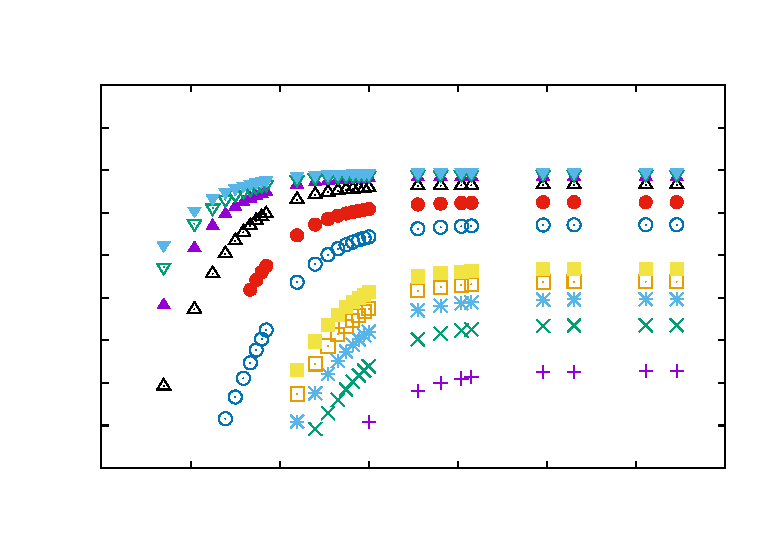
\includegraphics{../../Programming/sinking_bim_write_up/trunk/viscos_rat=01_pub}}%
    \gplfronttext
  \end{picture}%
\endgroup
}
        \caption{}
        \label{fig:viscos_rat=0.01}
      \end{subfigure}
      ~
      \begin{subfigure}[b]{0.45\textwidth}
        \resizebox{\textwidth}{!}{\Large % GNUPLOT: LaTeX picture with Postscript
\begingroup
  \makeatletter
  \providecommand\color[2][]{%
    \GenericError{(gnuplot) \space\space\space\@spaces}{%
      Package color not loaded in conjunction with
      terminal option `colourtext'%
    }{See the gnuplot documentation for explanation.%
    }{Either use 'blacktext' in gnuplot or load the package
      color.sty in LaTeX.}%
    \renewcommand\color[2][]{}%
  }%
  \providecommand\includegraphics[2][]{%
    \GenericError{(gnuplot) \space\space\space\@spaces}{%
      Package graphicx or graphics not loaded%
    }{See the gnuplot documentation for explanation.%
    }{The gnuplot epslatex terminal needs graphicx.sty or graphics.sty.}%
    \renewcommand\includegraphics[2][]{}%
  }%
  \providecommand\rotatebox[2]{#2}%
  \@ifundefined{ifGPcolor}{%
    \newif\ifGPcolor
    \GPcolorfalse
  }{}%
  \@ifundefined{ifGPblacktext}{%
    \newif\ifGPblacktext
    \GPblacktexttrue
  }{}%
  % define a \g@addto@macro without @ in the name:
  \let\gplgaddtomacro\g@addto@macro
  % define empty templates for all commands taking text:
  \gdef\gplbacktext{}%
  \gdef\gplfronttext{}%
  \makeatother
  \ifGPblacktext
    % no textcolor at all
    \def\colorrgb#1{}%
    \def\colorgray#1{}%
  \else
    % gray or color?
    \ifGPcolor
      \def\colorrgb#1{\color[rgb]{#1}}%
      \def\colorgray#1{\color[gray]{#1}}%
      \expandafter\def\csname LTw\endcsname{\color{white}}%
      \expandafter\def\csname LTb\endcsname{\color{black}}%
      \expandafter\def\csname LTa\endcsname{\color{black}}%
      \expandafter\def\csname LT0\endcsname{\color[rgb]{1,0,0}}%
      \expandafter\def\csname LT1\endcsname{\color[rgb]{0,1,0}}%
      \expandafter\def\csname LT2\endcsname{\color[rgb]{0,0,1}}%
      \expandafter\def\csname LT3\endcsname{\color[rgb]{1,0,1}}%
      \expandafter\def\csname LT4\endcsname{\color[rgb]{0,1,1}}%
      \expandafter\def\csname LT5\endcsname{\color[rgb]{1,1,0}}%
      \expandafter\def\csname LT6\endcsname{\color[rgb]{0,0,0}}%
      \expandafter\def\csname LT7\endcsname{\color[rgb]{1,0.3,0}}%
      \expandafter\def\csname LT8\endcsname{\color[rgb]{0.5,0.5,0.5}}%
    \else
      % gray
      \def\colorrgb#1{\color{black}}%
      \def\colorgray#1{\color[gray]{#1}}%
      \expandafter\def\csname LTw\endcsname{\color{white}}%
      \expandafter\def\csname LTb\endcsname{\color{black}}%
      \expandafter\def\csname LTa\endcsname{\color{black}}%
      \expandafter\def\csname LT0\endcsname{\color{black}}%
      \expandafter\def\csname LT1\endcsname{\color{black}}%
      \expandafter\def\csname LT2\endcsname{\color{black}}%
      \expandafter\def\csname LT3\endcsname{\color{black}}%
      \expandafter\def\csname LT4\endcsname{\color{black}}%
      \expandafter\def\csname LT5\endcsname{\color{black}}%
      \expandafter\def\csname LT6\endcsname{\color{black}}%
      \expandafter\def\csname LT7\endcsname{\color{black}}%
      \expandafter\def\csname LT8\endcsname{\color{black}}%
    \fi
  \fi
    \setlength{\unitlength}{0.0500bp}%
    \ifx\gptboxheight\undefined%
      \newlength{\gptboxheight}%
      \newlength{\gptboxwidth}%
      \newsavebox{\gptboxtext}%
    \fi%
    \setlength{\fboxrule}{0.5pt}%
    \setlength{\fboxsep}{1pt}%
\begin{picture}(7200.00,5040.00)%
    \gplgaddtomacro\gplbacktext{%
      \csname LTb\endcsname%
      \put(682,704){\makebox(0,0)[r]{\strut{}$0$}}%
      \put(682,1112){\makebox(0,0)[r]{\strut{}$2$}}%
      \put(682,1521){\makebox(0,0)[r]{\strut{}$4$}}%
      \put(682,1929){\makebox(0,0)[r]{\strut{}$6$}}%
      \put(682,2337){\makebox(0,0)[r]{\strut{}$8$}}%
      \put(682,2746){\makebox(0,0)[r]{\strut{}$10$}}%
      \put(682,3154){\makebox(0,0)[r]{\strut{}$12$}}%
      \put(682,3562){\makebox(0,0)[r]{\strut{}$14$}}%
      \put(682,3971){\makebox(0,0)[r]{\strut{}$16$}}%
      \put(682,4379){\makebox(0,0)[r]{\strut{}$18$}}%
      \put(814,484){\makebox(0,0){\strut{}$-6$}}%
      \put(1670,484){\makebox(0,0){\strut{}$-4$}}%
      \put(2525,484){\makebox(0,0){\strut{}$-2$}}%
      \put(3381,484){\makebox(0,0){\strut{}$0$}}%
      \put(4236,484){\makebox(0,0){\strut{}$2$}}%
      \put(5092,484){\makebox(0,0){\strut{}$4$}}%
      \put(5947,484){\makebox(0,0){\strut{}$6$}}%
      \put(6803,484){\makebox(0,0){\strut{}$8$}}%
    }%
    \gplgaddtomacro\gplfronttext{%
      \csname LTb\endcsname%
      \put(176,2541){\rotatebox{-270}{\makebox(0,0){\strut{}$V$}}}%
      \put(3808,154){\makebox(0,0){\strut{}$\ln\Bo$}}%
      \put(3808,4709){\makebox(0,0){\strut{}$\lambda = 0.03$}}%
      \put(3712,4151){\makebox(0,0){\strut{}$D$}}%
      \csname LTb\endcsname%
      \put(1474,3931){\makebox(0,0)[r]{\strut{}4}}%
      \csname LTb\endcsname%
      \put(1474,3601){\makebox(0,0)[r]{\strut{}8}}%
      \csname LTb\endcsname%
      \put(1474,3271){\makebox(0,0)[r]{\strut{}12}}%
      \csname LTb\endcsname%
      \put(2857,3931){\makebox(0,0)[r]{\strut{}16}}%
      \csname LTb\endcsname%
      \put(2857,3601){\makebox(0,0)[r]{\strut{}20}}%
      \csname LTb\endcsname%
      \put(2857,3271){\makebox(0,0)[r]{\strut{}50}}%
      \csname LTb\endcsname%
      \put(4240,3931){\makebox(0,0)[r]{\strut{}100}}%
      \csname LTb\endcsname%
      \put(4240,3601){\makebox(0,0)[r]{\strut{}250}}%
      \csname LTb\endcsname%
      \put(4240,3271){\makebox(0,0)[r]{\strut{}500}}%
      \csname LTb\endcsname%
      \put(5623,3931){\makebox(0,0)[r]{\strut{}750}}%
      \csname LTb\endcsname%
      \put(5623,3601){\makebox(0,0)[r]{\strut{}1000}}%
    }%
    \gplbacktext
    \put(0,0){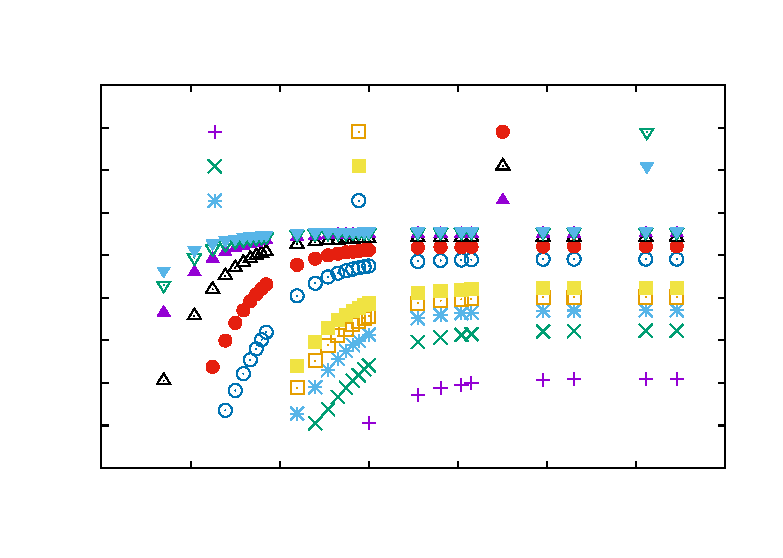
\includegraphics{../../Programming/sinking_bim_write_up/trunk/viscos_rat=03_pub}}%
    \gplfronttext
  \end{picture}%
\endgroup
}
        \caption{}
        \label{fig:mdr=viscos_rat=0.03}
      \end{subfigure}
      \caption{Dependence of entrained volume $V$ on $\Bo$ for different $D$ for a) $\lambda = 0.001$, b) $\lambda = 0.005$, c) $\lambda = 0.01$ and d) $\lambda = 0.03$. At small $\Bo$ there seems to be a linear relationship between $V$ and $\ln\Bo$ but as $\Bo$ increases, $V$ becomes independent of $\Bo$. }\label{fig:viscos_snap}
    \end{figure}

In magmas, the IFt $\sigma$ between two melts is expected to be equal to zero or very small (melts of different compositions are miscible). Therefore, in magmatic systems $\Bo \to \infty$. Motivated by this, figure~\ref{fig:highBo} shows the dependence of $V$ on $\lambda$ and $D$ for $\Bo = 1000$, which as can be seen from figures~\ref{fig:mdr_snap} and~\ref{fig:viscos_snap} is well into the regime where $V$ is independent of $\Bo$. Hence, these results can be considered the same as for when $\Bo \to \infty$. As seen in figure~\ref{fig:highBo_viscos}, for small values of $D$ ($\leq 3.5$) $V$ is nearly independent of $\lambda$. However, as $D$ increases, it is seen that $V$ decreases with $\lambda$. These features can also be seen in figure~\ref{fig:highBo_mdr} where it appears that the dependence on $D$ can be split into two regimes. For $\ln D$ between 0 and some critical value, $V \sim \ln D$. For $\lambda = 0.001$, this critical value is approximately 3, and this decreases to 1.4 for $\lambda = 0.05$. Above this critical value, the dependence on $D$ weakens, and it is possible that as $D \to \infty$, $V$ becomes independent of $D$, although further simulations at higher $D$ would be needed to verify this.

    \begin{figure}
      \centering
      \begin{subfigure}[b]{0.45\textwidth}
        \resizebox{\textwidth}{!}{\Large % GNUPLOT: LaTeX picture with Postscript
\begingroup
  \makeatletter
  \providecommand\color[2][]{%
    \GenericError{(gnuplot) \space\space\space\@spaces}{%
      Package color not loaded in conjunction with
      terminal option `colourtext'%
    }{See the gnuplot documentation for explanation.%
    }{Either use 'blacktext' in gnuplot or load the package
      color.sty in LaTeX.}%
    \renewcommand\color[2][]{}%
  }%
  \providecommand\includegraphics[2][]{%
    \GenericError{(gnuplot) \space\space\space\@spaces}{%
      Package graphicx or graphics not loaded%
    }{See the gnuplot documentation for explanation.%
    }{The gnuplot epslatex terminal needs graphicx.sty or graphics.sty.}%
    \renewcommand\includegraphics[2][]{}%
  }%
  \providecommand\rotatebox[2]{#2}%
  \@ifundefined{ifGPcolor}{%
    \newif\ifGPcolor
    \GPcolorfalse
  }{}%
  \@ifundefined{ifGPblacktext}{%
    \newif\ifGPblacktext
    \GPblacktexttrue
  }{}%
  % define a \g@addto@macro without @ in the name:
  \let\gplgaddtomacro\g@addto@macro
  % define empty templates for all commands taking text:
  \gdef\gplbacktext{}%
  \gdef\gplfronttext{}%
  \makeatother
  \ifGPblacktext
    % no textcolor at all
    \def\colorrgb#1{}%
    \def\colorgray#1{}%
  \else
    % gray or color?
    \ifGPcolor
      \def\colorrgb#1{\color[rgb]{#1}}%
      \def\colorgray#1{\color[gray]{#1}}%
      \expandafter\def\csname LTw\endcsname{\color{white}}%
      \expandafter\def\csname LTb\endcsname{\color{black}}%
      \expandafter\def\csname LTa\endcsname{\color{black}}%
      \expandafter\def\csname LT0\endcsname{\color[rgb]{1,0,0}}%
      \expandafter\def\csname LT1\endcsname{\color[rgb]{0,1,0}}%
      \expandafter\def\csname LT2\endcsname{\color[rgb]{0,0,1}}%
      \expandafter\def\csname LT3\endcsname{\color[rgb]{1,0,1}}%
      \expandafter\def\csname LT4\endcsname{\color[rgb]{0,1,1}}%
      \expandafter\def\csname LT5\endcsname{\color[rgb]{1,1,0}}%
      \expandafter\def\csname LT6\endcsname{\color[rgb]{0,0,0}}%
      \expandafter\def\csname LT7\endcsname{\color[rgb]{1,0.3,0}}%
      \expandafter\def\csname LT8\endcsname{\color[rgb]{0.5,0.5,0.5}}%
    \else
      % gray
      \def\colorrgb#1{\color{black}}%
      \def\colorgray#1{\color[gray]{#1}}%
      \expandafter\def\csname LTw\endcsname{\color{white}}%
      \expandafter\def\csname LTb\endcsname{\color{black}}%
      \expandafter\def\csname LTa\endcsname{\color{black}}%
      \expandafter\def\csname LT0\endcsname{\color{black}}%
      \expandafter\def\csname LT1\endcsname{\color{black}}%
      \expandafter\def\csname LT2\endcsname{\color{black}}%
      \expandafter\def\csname LT3\endcsname{\color{black}}%
      \expandafter\def\csname LT4\endcsname{\color{black}}%
      \expandafter\def\csname LT5\endcsname{\color{black}}%
      \expandafter\def\csname LT6\endcsname{\color{black}}%
      \expandafter\def\csname LT7\endcsname{\color{black}}%
      \expandafter\def\csname LT8\endcsname{\color{black}}%
    \fi
  \fi
    \setlength{\unitlength}{0.0500bp}%
    \ifx\gptboxheight\undefined%
      \newlength{\gptboxheight}%
      \newlength{\gptboxwidth}%
      \newsavebox{\gptboxtext}%
    \fi%
    \setlength{\fboxrule}{0.5pt}%
    \setlength{\fboxsep}{1pt}%
\begin{picture}(7200.00,5040.00)%
    \gplgaddtomacro\gplbacktext{%
      \csname LTb\endcsname%
      \put(682,704){\makebox(0,0)[r]{\strut{}$0$}}%
      \put(682,1112){\makebox(0,0)[r]{\strut{}$2$}}%
      \put(682,1521){\makebox(0,0)[r]{\strut{}$4$}}%
      \put(682,1929){\makebox(0,0)[r]{\strut{}$6$}}%
      \put(682,2337){\makebox(0,0)[r]{\strut{}$8$}}%
      \put(682,2746){\makebox(0,0)[r]{\strut{}$10$}}%
      \put(682,3154){\makebox(0,0)[r]{\strut{}$12$}}%
      \put(682,3562){\makebox(0,0)[r]{\strut{}$14$}}%
      \put(682,3971){\makebox(0,0)[r]{\strut{}$16$}}%
      \put(682,4379){\makebox(0,0)[r]{\strut{}$18$}}%
      \put(814,484){\makebox(0,0){\strut{}$0$}}%
      \put(2012,484){\makebox(0,0){\strut{}$0.01$}}%
      \put(3210,484){\makebox(0,0){\strut{}$0.02$}}%
      \put(4407,484){\makebox(0,0){\strut{}$0.03$}}%
      \put(5605,484){\makebox(0,0){\strut{}$0.04$}}%
      \put(6803,484){\makebox(0,0){\strut{}$0.05$}}%
    }%
    \gplgaddtomacro\gplfronttext{%
      \csname LTb\endcsname%
      \put(176,2541){\rotatebox{-270}{\makebox(0,0){\strut{}$V$}}}%
      \put(3808,154){\makebox(0,0){\strut{}$\lambda$}}%
      \put(3808,4709){\makebox(0,0){\strut{}$\Bo = 1000$}}%
      \put(4596,4151){\makebox(0,0){\strut{}$D$}}%
      \csname LTb\endcsname%
      \put(3050,3931){\makebox(0,0)[r]{\strut{}1.5}}%
      \csname LTb\endcsname%
      \put(3050,3601){\makebox(0,0)[r]{\strut{}2.5}}%
      \csname LTb\endcsname%
      \put(3050,3271){\makebox(0,0)[r]{\strut{}3.5}}%
      \csname LTb\endcsname%
      \put(4433,3931){\makebox(0,0)[r]{\strut{}8}}%
      \csname LTb\endcsname%
      \put(4433,3601){\makebox(0,0)[r]{\strut{}12}}%
      \csname LTb\endcsname%
      \put(4433,3271){\makebox(0,0)[r]{\strut{}20}}%
      \csname LTb\endcsname%
      \put(5816,3931){\makebox(0,0)[r]{\strut{}100}}%
      \csname LTb\endcsname%
      \put(5816,3601){\makebox(0,0)[r]{\strut{}500}}%
      \csname LTb\endcsname%
      \put(5816,3271){\makebox(0,0)[r]{\strut{}1000}}%
    }%
    \gplbacktext
    \put(0,0){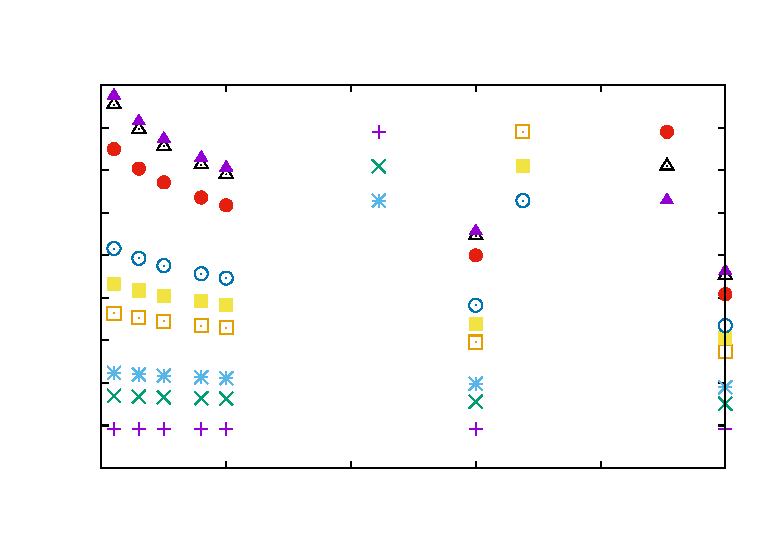
\includegraphics{../../Programming/sinking_bim_write_up/trunk/highBo_viscos_for_pub}}%
    \gplfronttext
  \end{picture}%
\endgroup
}
        \caption{}
        \label{fig:highBo_viscos}
      \end{subfigure}
      ~
      \begin{subfigure}[b]{0.45\textwidth}
        \resizebox{\textwidth}{!}{\Large % GNUPLOT: LaTeX picture with Postscript
\begingroup
  \makeatletter
  \providecommand\color[2][]{%
    \GenericError{(gnuplot) \space\space\space\@spaces}{%
      Package color not loaded in conjunction with
      terminal option `colourtext'%
    }{See the gnuplot documentation for explanation.%
    }{Either use 'blacktext' in gnuplot or load the package
      color.sty in LaTeX.}%
    \renewcommand\color[2][]{}%
  }%
  \providecommand\includegraphics[2][]{%
    \GenericError{(gnuplot) \space\space\space\@spaces}{%
      Package graphicx or graphics not loaded%
    }{See the gnuplot documentation for explanation.%
    }{The gnuplot epslatex terminal needs graphicx.sty or graphics.sty.}%
    \renewcommand\includegraphics[2][]{}%
  }%
  \providecommand\rotatebox[2]{#2}%
  \@ifundefined{ifGPcolor}{%
    \newif\ifGPcolor
    \GPcolorfalse
  }{}%
  \@ifundefined{ifGPblacktext}{%
    \newif\ifGPblacktext
    \GPblacktexttrue
  }{}%
  % define a \g@addto@macro without @ in the name:
  \let\gplgaddtomacro\g@addto@macro
  % define empty templates for all commands taking text:
  \gdef\gplbacktext{}%
  \gdef\gplfronttext{}%
  \makeatother
  \ifGPblacktext
    % no textcolor at all
    \def\colorrgb#1{}%
    \def\colorgray#1{}%
  \else
    % gray or color?
    \ifGPcolor
      \def\colorrgb#1{\color[rgb]{#1}}%
      \def\colorgray#1{\color[gray]{#1}}%
      \expandafter\def\csname LTw\endcsname{\color{white}}%
      \expandafter\def\csname LTb\endcsname{\color{black}}%
      \expandafter\def\csname LTa\endcsname{\color{black}}%
      \expandafter\def\csname LT0\endcsname{\color[rgb]{1,0,0}}%
      \expandafter\def\csname LT1\endcsname{\color[rgb]{0,1,0}}%
      \expandafter\def\csname LT2\endcsname{\color[rgb]{0,0,1}}%
      \expandafter\def\csname LT3\endcsname{\color[rgb]{1,0,1}}%
      \expandafter\def\csname LT4\endcsname{\color[rgb]{0,1,1}}%
      \expandafter\def\csname LT5\endcsname{\color[rgb]{1,1,0}}%
      \expandafter\def\csname LT6\endcsname{\color[rgb]{0,0,0}}%
      \expandafter\def\csname LT7\endcsname{\color[rgb]{1,0.3,0}}%
      \expandafter\def\csname LT8\endcsname{\color[rgb]{0.5,0.5,0.5}}%
    \else
      % gray
      \def\colorrgb#1{\color{black}}%
      \def\colorgray#1{\color[gray]{#1}}%
      \expandafter\def\csname LTw\endcsname{\color{white}}%
      \expandafter\def\csname LTb\endcsname{\color{black}}%
      \expandafter\def\csname LTa\endcsname{\color{black}}%
      \expandafter\def\csname LT0\endcsname{\color{black}}%
      \expandafter\def\csname LT1\endcsname{\color{black}}%
      \expandafter\def\csname LT2\endcsname{\color{black}}%
      \expandafter\def\csname LT3\endcsname{\color{black}}%
      \expandafter\def\csname LT4\endcsname{\color{black}}%
      \expandafter\def\csname LT5\endcsname{\color{black}}%
      \expandafter\def\csname LT6\endcsname{\color{black}}%
      \expandafter\def\csname LT7\endcsname{\color{black}}%
      \expandafter\def\csname LT8\endcsname{\color{black}}%
    \fi
  \fi
    \setlength{\unitlength}{0.0500bp}%
    \ifx\gptboxheight\undefined%
      \newlength{\gptboxheight}%
      \newlength{\gptboxwidth}%
      \newsavebox{\gptboxtext}%
    \fi%
    \setlength{\fboxrule}{0.5pt}%
    \setlength{\fboxsep}{1pt}%
\begin{picture}(7200.00,5040.00)%
    \gplgaddtomacro\gplbacktext{%
      \csname LTb\endcsname%
      \put(682,704){\makebox(0,0)[r]{\strut{}$0$}}%
      \put(682,1112){\makebox(0,0)[r]{\strut{}$2$}}%
      \put(682,1521){\makebox(0,0)[r]{\strut{}$4$}}%
      \put(682,1929){\makebox(0,0)[r]{\strut{}$6$}}%
      \put(682,2337){\makebox(0,0)[r]{\strut{}$8$}}%
      \put(682,2746){\makebox(0,0)[r]{\strut{}$10$}}%
      \put(682,3154){\makebox(0,0)[r]{\strut{}$12$}}%
      \put(682,3562){\makebox(0,0)[r]{\strut{}$14$}}%
      \put(682,3971){\makebox(0,0)[r]{\strut{}$16$}}%
      \put(682,4379){\makebox(0,0)[r]{\strut{}$18$}}%
      \put(1358,484){\makebox(0,0){\strut{}$1$}}%
      \put(2266,484){\makebox(0,0){\strut{}$2$}}%
      \put(3173,484){\makebox(0,0){\strut{}$3$}}%
      \put(4081,484){\makebox(0,0){\strut{}$4$}}%
      \put(4988,484){\makebox(0,0){\strut{}$5$}}%
      \put(5896,484){\makebox(0,0){\strut{}$6$}}%
      \put(6803,484){\makebox(0,0){\strut{}$7$}}%
    }%
    \gplgaddtomacro\gplfronttext{%
      \csname LTb\endcsname%
      \put(176,2541){\rotatebox{-270}{\makebox(0,0){\strut{}$V$}}}%
      \put(3808,154){\makebox(0,0){\strut{}$\ln D$}}%
      \put(3808,4709){\makebox(0,0){\strut{}$\Bo = 1000$}}%
      \put(2461,4151){\makebox(0,0){\strut{}$\lambda$}}%
      \csname LTb\endcsname%
      \put(1606,3931){\makebox(0,0)[r]{\strut{}0.001}}%
      \csname LTb\endcsname%
      \put(1606,3601){\makebox(0,0)[r]{\strut{}0.003}}%
      \csname LTb\endcsname%
      \put(1606,3271){\makebox(0,0)[r]{\strut{}0.005}}%
      \csname LTb\endcsname%
      \put(1606,2941){\makebox(0,0)[r]{\strut{}0.008}}%
      \csname LTb\endcsname%
      \put(3121,3931){\makebox(0,0)[r]{\strut{}0.01}}%
      \csname LTb\endcsname%
      \put(3121,3601){\makebox(0,0)[r]{\strut{}0.03}}%
      \csname LTb\endcsname%
      \put(3121,3271){\makebox(0,0)[r]{\strut{}0.05}}%
    }%
    \gplbacktext
    \put(0,0){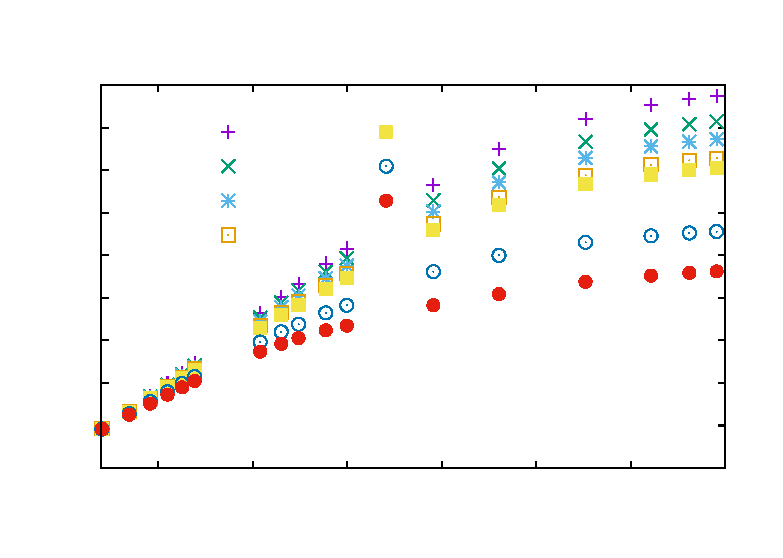
\includegraphics{../../Programming/sinking_bim_write_up/trunk/highBo_mdr_for_pub}}%
    \gplfronttext
  \end{picture}%
\endgroup
}
        \caption{}
        \label{fig:highBo_mdr}
      \end{subfigure}
      \caption{Dependence of $V$ on a) $\lambda$ for different $D$ and b) $D$ for different $\lambda$, for $\Bo = 1000$, which is in the regime where $V$ is independent of $\Bo$.}\label{fig:highBo}
    \end{figure}

\subsubsection{Sinking Timescale}
\label{subsubsec:sink_time}

The sinking timescale $t_{\text{s}}$ is defined as the time between the sphere first touching the plane of the undeformed interface and the moment at which the sphere loses contact with the bulk of the upper phase i.e. when the tail snaps. Within the BIM, this is interpretted as the moment at which the separation between the two branches of the interface becomes smaller than the separation between the points use to discretise it. Figure~\ref{fig:mdr_time} shows the dependence of the sinking time on the Bond number, for different values of the MDR and viscosity ratio. It is observed that the function $t_{\text{s}} = t_{\text{s}}(\Bo, D, \lambda)$ is not simple. For all values of $D$ and $\Bo$, the larger the value of the viscosity ratio, the longer the sinking time. Additionally, for all values of $D$, as $\Bo$ approaches the floating transition, the time taken for sinking tends to infinity, and as $\Bo \to \infty$ the sinking time becomes independent of $\Bo$. However, the behaviour is complicated for intermediate value of $\Bo$. For $D = 8$, the decrease in sinking time with $\Bo$ is monotonic. However as $D$ increases, a minimum in the sinking time as a function of $\Bo$ appears. This minimum only appears for larger values of the viscosity ratio and becomes more pronounced as the viscosity ratio increases. For the case $D = 1000$, it is inferred that the minimum in the curve for $\lambda = 0.03$ occurs at a vlaue of $\Bo < 0.01$ (the smallest Bond number investigated).

    \begin{figure}
      \centering
      \begin{subfigure}[b]{0.45\textwidth}
        \resizebox{\textwidth}{!}{\Large % GNUPLOT: LaTeX picture with Postscript
\begingroup
  \makeatletter
  \providecommand\color[2][]{%
    \GenericError{(gnuplot) \space\space\space\@spaces}{%
      Package color not loaded in conjunction with
      terminal option `colourtext'%
    }{See the gnuplot documentation for explanation.%
    }{Either use 'blacktext' in gnuplot or load the package
      color.sty in LaTeX.}%
    \renewcommand\color[2][]{}%
  }%
  \providecommand\includegraphics[2][]{%
    \GenericError{(gnuplot) \space\space\space\@spaces}{%
      Package graphicx or graphics not loaded%
    }{See the gnuplot documentation for explanation.%
    }{The gnuplot epslatex terminal needs graphicx.sty or graphics.sty.}%
    \renewcommand\includegraphics[2][]{}%
  }%
  \providecommand\rotatebox[2]{#2}%
  \@ifundefined{ifGPcolor}{%
    \newif\ifGPcolor
    \GPcolorfalse
  }{}%
  \@ifundefined{ifGPblacktext}{%
    \newif\ifGPblacktext
    \GPblacktexttrue
  }{}%
  % define a \g@addto@macro without @ in the name:
  \let\gplgaddtomacro\g@addto@macro
  % define empty templates for all commands taking text:
  \gdef\gplbacktext{}%
  \gdef\gplfronttext{}%
  \makeatother
  \ifGPblacktext
    % no textcolor at all
    \def\colorrgb#1{}%
    \def\colorgray#1{}%
  \else
    % gray or color?
    \ifGPcolor
      \def\colorrgb#1{\color[rgb]{#1}}%
      \def\colorgray#1{\color[gray]{#1}}%
      \expandafter\def\csname LTw\endcsname{\color{white}}%
      \expandafter\def\csname LTb\endcsname{\color{black}}%
      \expandafter\def\csname LTa\endcsname{\color{black}}%
      \expandafter\def\csname LT0\endcsname{\color[rgb]{1,0,0}}%
      \expandafter\def\csname LT1\endcsname{\color[rgb]{0,1,0}}%
      \expandafter\def\csname LT2\endcsname{\color[rgb]{0,0,1}}%
      \expandafter\def\csname LT3\endcsname{\color[rgb]{1,0,1}}%
      \expandafter\def\csname LT4\endcsname{\color[rgb]{0,1,1}}%
      \expandafter\def\csname LT5\endcsname{\color[rgb]{1,1,0}}%
      \expandafter\def\csname LT6\endcsname{\color[rgb]{0,0,0}}%
      \expandafter\def\csname LT7\endcsname{\color[rgb]{1,0.3,0}}%
      \expandafter\def\csname LT8\endcsname{\color[rgb]{0.5,0.5,0.5}}%
    \else
      % gray
      \def\colorrgb#1{\color{black}}%
      \def\colorgray#1{\color[gray]{#1}}%
      \expandafter\def\csname LTw\endcsname{\color{white}}%
      \expandafter\def\csname LTb\endcsname{\color{black}}%
      \expandafter\def\csname LTa\endcsname{\color{black}}%
      \expandafter\def\csname LT0\endcsname{\color{black}}%
      \expandafter\def\csname LT1\endcsname{\color{black}}%
      \expandafter\def\csname LT2\endcsname{\color{black}}%
      \expandafter\def\csname LT3\endcsname{\color{black}}%
      \expandafter\def\csname LT4\endcsname{\color{black}}%
      \expandafter\def\csname LT5\endcsname{\color{black}}%
      \expandafter\def\csname LT6\endcsname{\color{black}}%
      \expandafter\def\csname LT7\endcsname{\color{black}}%
      \expandafter\def\csname LT8\endcsname{\color{black}}%
    \fi
  \fi
    \setlength{\unitlength}{0.0500bp}%
    \ifx\gptboxheight\undefined%
      \newlength{\gptboxheight}%
      \newlength{\gptboxwidth}%
      \newsavebox{\gptboxtext}%
    \fi%
    \setlength{\fboxrule}{0.5pt}%
    \setlength{\fboxsep}{1pt}%
\begin{picture}(7200.00,5040.00)%
    \gplgaddtomacro\gplbacktext{%
      \csname LTb\endcsname%
      \put(682,704){\makebox(0,0)[r]{\strut{}$5$}}%
      \put(682,1317){\makebox(0,0)[r]{\strut{}$10$}}%
      \put(682,1929){\makebox(0,0)[r]{\strut{}$15$}}%
      \put(682,2542){\makebox(0,0)[r]{\strut{}$20$}}%
      \put(682,3154){\makebox(0,0)[r]{\strut{}$25$}}%
      \put(682,3767){\makebox(0,0)[r]{\strut{}$30$}}%
      \put(682,4379){\makebox(0,0)[r]{\strut{}$35$}}%
      \put(814,484){\makebox(0,0){\strut{}$-6$}}%
      \put(1670,484){\makebox(0,0){\strut{}$-4$}}%
      \put(2525,484){\makebox(0,0){\strut{}$-2$}}%
      \put(3381,484){\makebox(0,0){\strut{}$0$}}%
      \put(4236,484){\makebox(0,0){\strut{}$2$}}%
      \put(5092,484){\makebox(0,0){\strut{}$4$}}%
      \put(5947,484){\makebox(0,0){\strut{}$6$}}%
      \put(6803,484){\makebox(0,0){\strut{}$8$}}%
    }%
    \gplgaddtomacro\gplfronttext{%
      \csname LTb\endcsname%
      \put(176,2541){\rotatebox{-270}{\makebox(0,0){\strut{}$t_{\text{s}}$}}}%
      \put(3808,154){\makebox(0,0){\strut{}$\ln \Bo$}}%
      \put(3808,4709){\makebox(0,0){\strut{}$D = 8$}}%
      \put(5913,4151){\makebox(0,0){\strut{}$\lambda$}}%
      \csname LTb\endcsname%
      \put(5816,3931){\makebox(0,0)[r]{\strut{}0.001}}%
      \csname LTb\endcsname%
      \put(5816,3601){\makebox(0,0)[r]{\strut{}0.003}}%
      \csname LTb\endcsname%
      \put(5816,3271){\makebox(0,0)[r]{\strut{}0.005}}%
      \csname LTb\endcsname%
      \put(5816,2941){\makebox(0,0)[r]{\strut{}0.008}}%
      \csname LTb\endcsname%
      \put(5816,2611){\makebox(0,0)[r]{\strut{}0.01}}%
      \csname LTb\endcsname%
      \put(5816,2281){\makebox(0,0)[r]{\strut{}0.03}}%
    }%
    \gplbacktext
    \put(0,0){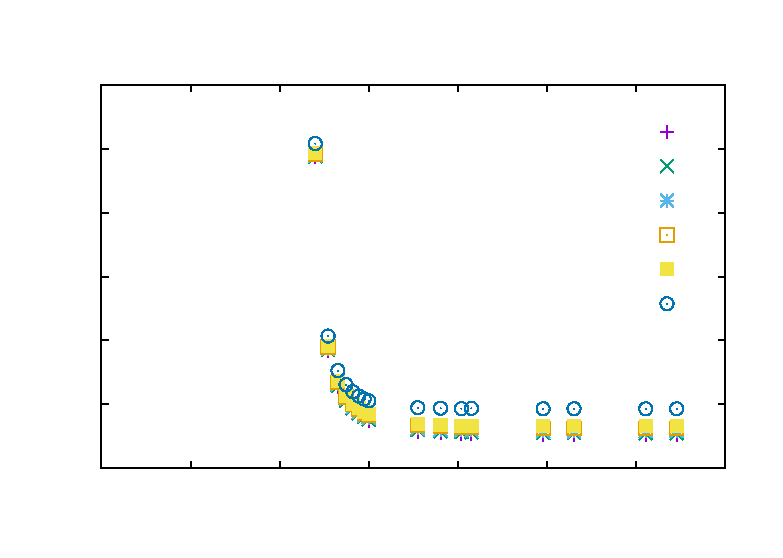
\includegraphics{../../Programming/sinking_bim_write_up/trunk/mdr=8_time}}%
    \gplfronttext
  \end{picture}%
\endgroup
}
        \caption{}
        \label{fig:mdr=8_time}
      \end{subfigure}
      ~
      \begin{subfigure}[b]{0.45\textwidth}
        \resizebox{\textwidth}{!}{\Large % GNUPLOT: LaTeX picture with Postscript
\begingroup
  \makeatletter
  \providecommand\color[2][]{%
    \GenericError{(gnuplot) \space\space\space\@spaces}{%
      Package color not loaded in conjunction with
      terminal option `colourtext'%
    }{See the gnuplot documentation for explanation.%
    }{Either use 'blacktext' in gnuplot or load the package
      color.sty in LaTeX.}%
    \renewcommand\color[2][]{}%
  }%
  \providecommand\includegraphics[2][]{%
    \GenericError{(gnuplot) \space\space\space\@spaces}{%
      Package graphicx or graphics not loaded%
    }{See the gnuplot documentation for explanation.%
    }{The gnuplot epslatex terminal needs graphicx.sty or graphics.sty.}%
    \renewcommand\includegraphics[2][]{}%
  }%
  \providecommand\rotatebox[2]{#2}%
  \@ifundefined{ifGPcolor}{%
    \newif\ifGPcolor
    \GPcolorfalse
  }{}%
  \@ifundefined{ifGPblacktext}{%
    \newif\ifGPblacktext
    \GPblacktexttrue
  }{}%
  % define a \g@addto@macro without @ in the name:
  \let\gplgaddtomacro\g@addto@macro
  % define empty templates for all commands taking text:
  \gdef\gplbacktext{}%
  \gdef\gplfronttext{}%
  \makeatother
  \ifGPblacktext
    % no textcolor at all
    \def\colorrgb#1{}%
    \def\colorgray#1{}%
  \else
    % gray or color?
    \ifGPcolor
      \def\colorrgb#1{\color[rgb]{#1}}%
      \def\colorgray#1{\color[gray]{#1}}%
      \expandafter\def\csname LTw\endcsname{\color{white}}%
      \expandafter\def\csname LTb\endcsname{\color{black}}%
      \expandafter\def\csname LTa\endcsname{\color{black}}%
      \expandafter\def\csname LT0\endcsname{\color[rgb]{1,0,0}}%
      \expandafter\def\csname LT1\endcsname{\color[rgb]{0,1,0}}%
      \expandafter\def\csname LT2\endcsname{\color[rgb]{0,0,1}}%
      \expandafter\def\csname LT3\endcsname{\color[rgb]{1,0,1}}%
      \expandafter\def\csname LT4\endcsname{\color[rgb]{0,1,1}}%
      \expandafter\def\csname LT5\endcsname{\color[rgb]{1,1,0}}%
      \expandafter\def\csname LT6\endcsname{\color[rgb]{0,0,0}}%
      \expandafter\def\csname LT7\endcsname{\color[rgb]{1,0.3,0}}%
      \expandafter\def\csname LT8\endcsname{\color[rgb]{0.5,0.5,0.5}}%
    \else
      % gray
      \def\colorrgb#1{\color{black}}%
      \def\colorgray#1{\color[gray]{#1}}%
      \expandafter\def\csname LTw\endcsname{\color{white}}%
      \expandafter\def\csname LTb\endcsname{\color{black}}%
      \expandafter\def\csname LTa\endcsname{\color{black}}%
      \expandafter\def\csname LT0\endcsname{\color{black}}%
      \expandafter\def\csname LT1\endcsname{\color{black}}%
      \expandafter\def\csname LT2\endcsname{\color{black}}%
      \expandafter\def\csname LT3\endcsname{\color{black}}%
      \expandafter\def\csname LT4\endcsname{\color{black}}%
      \expandafter\def\csname LT5\endcsname{\color{black}}%
      \expandafter\def\csname LT6\endcsname{\color{black}}%
      \expandafter\def\csname LT7\endcsname{\color{black}}%
      \expandafter\def\csname LT8\endcsname{\color{black}}%
    \fi
  \fi
    \setlength{\unitlength}{0.0500bp}%
    \ifx\gptboxheight\undefined%
      \newlength{\gptboxheight}%
      \newlength{\gptboxwidth}%
      \newsavebox{\gptboxtext}%
    \fi%
    \setlength{\fboxrule}{0.5pt}%
    \setlength{\fboxsep}{1pt}%
\begin{picture}(7200.00,5040.00)%
    \gplgaddtomacro\gplbacktext{%
      \csname LTb\endcsname%
      \put(682,704){\makebox(0,0)[r]{\strut{}$6$}}%
      \put(682,1163){\makebox(0,0)[r]{\strut{}$8$}}%
      \put(682,1623){\makebox(0,0)[r]{\strut{}$10$}}%
      \put(682,2082){\makebox(0,0)[r]{\strut{}$12$}}%
      \put(682,2542){\makebox(0,0)[r]{\strut{}$14$}}%
      \put(682,3001){\makebox(0,0)[r]{\strut{}$16$}}%
      \put(682,3460){\makebox(0,0)[r]{\strut{}$18$}}%
      \put(682,3920){\makebox(0,0)[r]{\strut{}$20$}}%
      \put(682,4379){\makebox(0,0)[r]{\strut{}$22$}}%
      \put(814,484){\makebox(0,0){\strut{}$-6$}}%
      \put(1670,484){\makebox(0,0){\strut{}$-4$}}%
      \put(2525,484){\makebox(0,0){\strut{}$-2$}}%
      \put(3381,484){\makebox(0,0){\strut{}$0$}}%
      \put(4236,484){\makebox(0,0){\strut{}$2$}}%
      \put(5092,484){\makebox(0,0){\strut{}$4$}}%
      \put(5947,484){\makebox(0,0){\strut{}$6$}}%
      \put(6803,484){\makebox(0,0){\strut{}$8$}}%
    }%
    \gplgaddtomacro\gplfronttext{%
      \csname LTb\endcsname%
      \put(176,2541){\rotatebox{-270}{\makebox(0,0){\strut{}$t_{\text{s}}$}}}%
      \put(3808,154){\makebox(0,0){\strut{}$\ln \Bo$}}%
      \put(3808,4709){\makebox(0,0){\strut{}$D = 50$}}%
    }%
    \gplbacktext
    \put(0,0){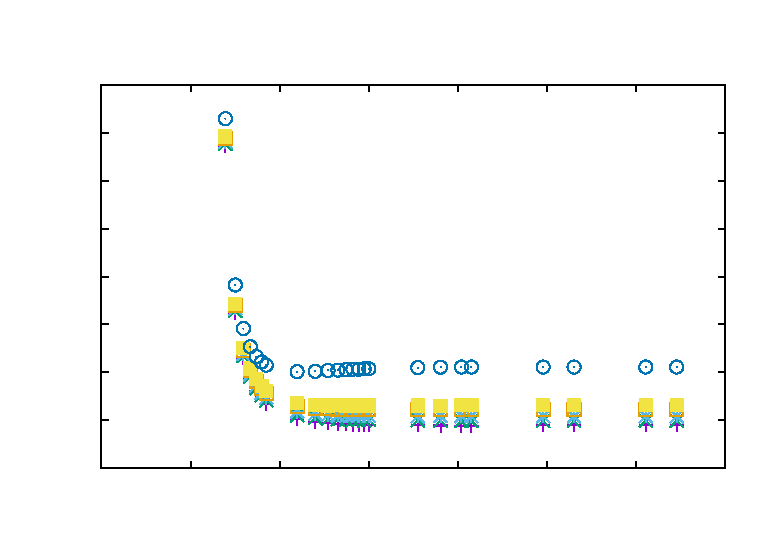
\includegraphics{../../Programming/sinking_bim_write_up/trunk/mdr=50_time}}%
    \gplfronttext
  \end{picture}%
\endgroup
}
        \caption{}
        \label{fig:mdr=50_time}
      \end{subfigure}
      
      \begin{subfigure}[b]{0.45\textwidth}
        \resizebox{\textwidth}{!}{\Large % GNUPLOT: LaTeX picture with Postscript
\begingroup
  \makeatletter
  \providecommand\color[2][]{%
    \GenericError{(gnuplot) \space\space\space\@spaces}{%
      Package color not loaded in conjunction with
      terminal option `colourtext'%
    }{See the gnuplot documentation for explanation.%
    }{Either use 'blacktext' in gnuplot or load the package
      color.sty in LaTeX.}%
    \renewcommand\color[2][]{}%
  }%
  \providecommand\includegraphics[2][]{%
    \GenericError{(gnuplot) \space\space\space\@spaces}{%
      Package graphicx or graphics not loaded%
    }{See the gnuplot documentation for explanation.%
    }{The gnuplot epslatex terminal needs graphicx.sty or graphics.sty.}%
    \renewcommand\includegraphics[2][]{}%
  }%
  \providecommand\rotatebox[2]{#2}%
  \@ifundefined{ifGPcolor}{%
    \newif\ifGPcolor
    \GPcolorfalse
  }{}%
  \@ifundefined{ifGPblacktext}{%
    \newif\ifGPblacktext
    \GPblacktexttrue
  }{}%
  % define a \g@addto@macro without @ in the name:
  \let\gplgaddtomacro\g@addto@macro
  % define empty templates for all commands taking text:
  \gdef\gplbacktext{}%
  \gdef\gplfronttext{}%
  \makeatother
  \ifGPblacktext
    % no textcolor at all
    \def\colorrgb#1{}%
    \def\colorgray#1{}%
  \else
    % gray or color?
    \ifGPcolor
      \def\colorrgb#1{\color[rgb]{#1}}%
      \def\colorgray#1{\color[gray]{#1}}%
      \expandafter\def\csname LTw\endcsname{\color{white}}%
      \expandafter\def\csname LTb\endcsname{\color{black}}%
      \expandafter\def\csname LTa\endcsname{\color{black}}%
      \expandafter\def\csname LT0\endcsname{\color[rgb]{1,0,0}}%
      \expandafter\def\csname LT1\endcsname{\color[rgb]{0,1,0}}%
      \expandafter\def\csname LT2\endcsname{\color[rgb]{0,0,1}}%
      \expandafter\def\csname LT3\endcsname{\color[rgb]{1,0,1}}%
      \expandafter\def\csname LT4\endcsname{\color[rgb]{0,1,1}}%
      \expandafter\def\csname LT5\endcsname{\color[rgb]{1,1,0}}%
      \expandafter\def\csname LT6\endcsname{\color[rgb]{0,0,0}}%
      \expandafter\def\csname LT7\endcsname{\color[rgb]{1,0.3,0}}%
      \expandafter\def\csname LT8\endcsname{\color[rgb]{0.5,0.5,0.5}}%
    \else
      % gray
      \def\colorrgb#1{\color{black}}%
      \def\colorgray#1{\color[gray]{#1}}%
      \expandafter\def\csname LTw\endcsname{\color{white}}%
      \expandafter\def\csname LTb\endcsname{\color{black}}%
      \expandafter\def\csname LTa\endcsname{\color{black}}%
      \expandafter\def\csname LT0\endcsname{\color{black}}%
      \expandafter\def\csname LT1\endcsname{\color{black}}%
      \expandafter\def\csname LT2\endcsname{\color{black}}%
      \expandafter\def\csname LT3\endcsname{\color{black}}%
      \expandafter\def\csname LT4\endcsname{\color{black}}%
      \expandafter\def\csname LT5\endcsname{\color{black}}%
      \expandafter\def\csname LT6\endcsname{\color{black}}%
      \expandafter\def\csname LT7\endcsname{\color{black}}%
      \expandafter\def\csname LT8\endcsname{\color{black}}%
    \fi
  \fi
    \setlength{\unitlength}{0.0500bp}%
    \ifx\gptboxheight\undefined%
      \newlength{\gptboxheight}%
      \newlength{\gptboxwidth}%
      \newsavebox{\gptboxtext}%
    \fi%
    \setlength{\fboxrule}{0.5pt}%
    \setlength{\fboxsep}{1pt}%
\begin{picture}(7200.00,5040.00)%
    \gplgaddtomacro\gplbacktext{%
      \csname LTb\endcsname%
      \put(946,704){\makebox(0,0)[r]{\strut{}$8$}}%
      \put(946,1163){\makebox(0,0)[r]{\strut{}$8.5$}}%
      \put(946,1623){\makebox(0,0)[r]{\strut{}$9$}}%
      \put(946,2082){\makebox(0,0)[r]{\strut{}$9.5$}}%
      \put(946,2542){\makebox(0,0)[r]{\strut{}$10$}}%
      \put(946,3001){\makebox(0,0)[r]{\strut{}$10.5$}}%
      \put(946,3460){\makebox(0,0)[r]{\strut{}$11$}}%
      \put(946,3920){\makebox(0,0)[r]{\strut{}$11.5$}}%
      \put(946,4379){\makebox(0,0)[r]{\strut{}$12$}}%
      \put(1078,484){\makebox(0,0){\strut{}$-6$}}%
      \put(1896,484){\makebox(0,0){\strut{}$-4$}}%
      \put(2714,484){\makebox(0,0){\strut{}$-2$}}%
      \put(3532,484){\makebox(0,0){\strut{}$0$}}%
      \put(4349,484){\makebox(0,0){\strut{}$2$}}%
      \put(5167,484){\makebox(0,0){\strut{}$4$}}%
      \put(5985,484){\makebox(0,0){\strut{}$6$}}%
      \put(6803,484){\makebox(0,0){\strut{}$8$}}%
    }%
    \gplgaddtomacro\gplfronttext{%
      \csname LTb\endcsname%
      \put(176,2541){\rotatebox{-270}{\makebox(0,0){\strut{}$t_{\text{s}}$}}}%
      \put(3940,154){\makebox(0,0){\strut{}$\ln \Bo$}}%
      \put(3940,4709){\makebox(0,0){\strut{}$D = 100$}}%
    }%
    \gplbacktext
    \put(0,0){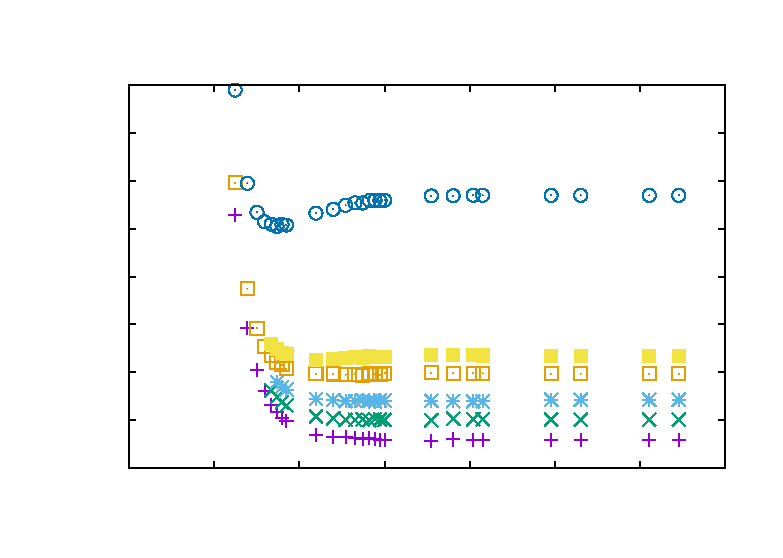
\includegraphics{../../Programming/sinking_bim_write_up/trunk/mdr=100_time}}%
    \gplfronttext
  \end{picture}%
\endgroup
}
        \caption{}
        \label{fig:mdr=100_time}
      \end{subfigure}
      ~
      \begin{subfigure}[b]{0.45\textwidth}
        \resizebox{\textwidth}{!}{\Large % GNUPLOT: LaTeX picture with Postscript
\begingroup
  \makeatletter
  \providecommand\color[2][]{%
    \GenericError{(gnuplot) \space\space\space\@spaces}{%
      Package color not loaded in conjunction with
      terminal option `colourtext'%
    }{See the gnuplot documentation for explanation.%
    }{Either use 'blacktext' in gnuplot or load the package
      color.sty in LaTeX.}%
    \renewcommand\color[2][]{}%
  }%
  \providecommand\includegraphics[2][]{%
    \GenericError{(gnuplot) \space\space\space\@spaces}{%
      Package graphicx or graphics not loaded%
    }{See the gnuplot documentation for explanation.%
    }{The gnuplot epslatex terminal needs graphicx.sty or graphics.sty.}%
    \renewcommand\includegraphics[2][]{}%
  }%
  \providecommand\rotatebox[2]{#2}%
  \@ifundefined{ifGPcolor}{%
    \newif\ifGPcolor
    \GPcolorfalse
  }{}%
  \@ifundefined{ifGPblacktext}{%
    \newif\ifGPblacktext
    \GPblacktexttrue
  }{}%
  % define a \g@addto@macro without @ in the name:
  \let\gplgaddtomacro\g@addto@macro
  % define empty templates for all commands taking text:
  \gdef\gplbacktext{}%
  \gdef\gplfronttext{}%
  \makeatother
  \ifGPblacktext
    % no textcolor at all
    \def\colorrgb#1{}%
    \def\colorgray#1{}%
  \else
    % gray or color?
    \ifGPcolor
      \def\colorrgb#1{\color[rgb]{#1}}%
      \def\colorgray#1{\color[gray]{#1}}%
      \expandafter\def\csname LTw\endcsname{\color{white}}%
      \expandafter\def\csname LTb\endcsname{\color{black}}%
      \expandafter\def\csname LTa\endcsname{\color{black}}%
      \expandafter\def\csname LT0\endcsname{\color[rgb]{1,0,0}}%
      \expandafter\def\csname LT1\endcsname{\color[rgb]{0,1,0}}%
      \expandafter\def\csname LT2\endcsname{\color[rgb]{0,0,1}}%
      \expandafter\def\csname LT3\endcsname{\color[rgb]{1,0,1}}%
      \expandafter\def\csname LT4\endcsname{\color[rgb]{0,1,1}}%
      \expandafter\def\csname LT5\endcsname{\color[rgb]{1,1,0}}%
      \expandafter\def\csname LT6\endcsname{\color[rgb]{0,0,0}}%
      \expandafter\def\csname LT7\endcsname{\color[rgb]{1,0.3,0}}%
      \expandafter\def\csname LT8\endcsname{\color[rgb]{0.5,0.5,0.5}}%
    \else
      % gray
      \def\colorrgb#1{\color{black}}%
      \def\colorgray#1{\color[gray]{#1}}%
      \expandafter\def\csname LTw\endcsname{\color{white}}%
      \expandafter\def\csname LTb\endcsname{\color{black}}%
      \expandafter\def\csname LTa\endcsname{\color{black}}%
      \expandafter\def\csname LT0\endcsname{\color{black}}%
      \expandafter\def\csname LT1\endcsname{\color{black}}%
      \expandafter\def\csname LT2\endcsname{\color{black}}%
      \expandafter\def\csname LT3\endcsname{\color{black}}%
      \expandafter\def\csname LT4\endcsname{\color{black}}%
      \expandafter\def\csname LT5\endcsname{\color{black}}%
      \expandafter\def\csname LT6\endcsname{\color{black}}%
      \expandafter\def\csname LT7\endcsname{\color{black}}%
      \expandafter\def\csname LT8\endcsname{\color{black}}%
    \fi
  \fi
    \setlength{\unitlength}{0.0500bp}%
    \ifx\gptboxheight\undefined%
      \newlength{\gptboxheight}%
      \newlength{\gptboxwidth}%
      \newsavebox{\gptboxtext}%
    \fi%
    \setlength{\fboxrule}{0.5pt}%
    \setlength{\fboxsep}{1pt}%
\begin{picture}(7200.00,5040.00)%
    \gplgaddtomacro\gplbacktext{%
      \csname LTb\endcsname%
      \put(946,704){\makebox(0,0)[r]{\strut{}$9$}}%
      \put(946,1229){\makebox(0,0)[r]{\strut{}$9.5$}}%
      \put(946,1754){\makebox(0,0)[r]{\strut{}$10$}}%
      \put(946,2279){\makebox(0,0)[r]{\strut{}$10.5$}}%
      \put(946,2804){\makebox(0,0)[r]{\strut{}$11$}}%
      \put(946,3329){\makebox(0,0)[r]{\strut{}$11.5$}}%
      \put(946,3854){\makebox(0,0)[r]{\strut{}$12$}}%
      \put(946,4379){\makebox(0,0)[r]{\strut{}$12.5$}}%
      \put(1078,484){\makebox(0,0){\strut{}$-6$}}%
      \put(1896,484){\makebox(0,0){\strut{}$-4$}}%
      \put(2714,484){\makebox(0,0){\strut{}$-2$}}%
      \put(3532,484){\makebox(0,0){\strut{}$0$}}%
      \put(4349,484){\makebox(0,0){\strut{}$2$}}%
      \put(5167,484){\makebox(0,0){\strut{}$4$}}%
      \put(5985,484){\makebox(0,0){\strut{}$6$}}%
      \put(6803,484){\makebox(0,0){\strut{}$8$}}%
    }%
    \gplgaddtomacro\gplfronttext{%
      \csname LTb\endcsname%
      \put(176,2541){\rotatebox{-270}{\makebox(0,0){\strut{}$t_{\text{s}}$}}}%
      \put(3940,154){\makebox(0,0){\strut{}$\ln \Bo$}}%
      \put(3940,4709){\makebox(0,0){\strut{}$D = 1000$}}%
    }%
    \gplbacktext
    \put(0,0){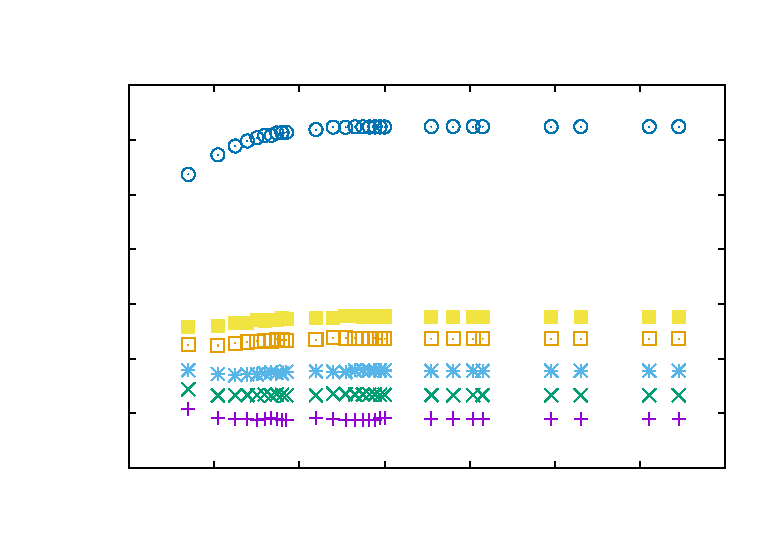
\includegraphics{../../Programming/sinking_bim_write_up/trunk/mdr=1000_time}}%
    \gplfronttext
  \end{picture}%
\endgroup
}
        \caption{}
        \label{fig:mdr=1000_time}
      \end{subfigure}
      \caption{Dependence of the sinking timescale $t_{\text{s}}$ on $\Bo$ for different $\lambda$ and a) $D = 8$, b) $D = 50$, c) $D = 100$ and d) $D = 1000$. Note the difference in vertical scale between the figures.}\label{fig:mdr_time}
    \end{figure}

Bearing in mind the application to mixing magmas, the high Bond number limit has been investigated (figure~\ref{fig:highBo_time}). As before, figure~\ref{fig:time_viscos} shows that an increase in the value of the viscosity ratio leads to an increase in the sinking timescale. Like with $\Bo$, the sinking timescale depends on $D$ in a non-monotonic fashion (figure~\ref{fig:time_mdr}). As $D \to 1$, $t_{\text{s}} \to \infty$ and as $D \to \infty$ the sinking timescale becomes independent of $D$. However, there is a local minimum in the value of $t_{\text{s}}$ at approximately $\ln D \approx 2$ ($D \approx 7.3$).

    \begin{figure}
      \centering
      \begin{subfigure}[b]{0.45\textwidth}
        \resizebox{\textwidth}{!}{\Large % GNUPLOT: LaTeX picture with Postscript
\begingroup
  \makeatletter
  \providecommand\color[2][]{%
    \GenericError{(gnuplot) \space\space\space\@spaces}{%
      Package color not loaded in conjunction with
      terminal option `colourtext'%
    }{See the gnuplot documentation for explanation.%
    }{Either use 'blacktext' in gnuplot or load the package
      color.sty in LaTeX.}%
    \renewcommand\color[2][]{}%
  }%
  \providecommand\includegraphics[2][]{%
    \GenericError{(gnuplot) \space\space\space\@spaces}{%
      Package graphicx or graphics not loaded%
    }{See the gnuplot documentation for explanation.%
    }{The gnuplot epslatex terminal needs graphicx.sty or graphics.sty.}%
    \renewcommand\includegraphics[2][]{}%
  }%
  \providecommand\rotatebox[2]{#2}%
  \@ifundefined{ifGPcolor}{%
    \newif\ifGPcolor
    \GPcolorfalse
  }{}%
  \@ifundefined{ifGPblacktext}{%
    \newif\ifGPblacktext
    \GPblacktexttrue
  }{}%
  % define a \g@addto@macro without @ in the name:
  \let\gplgaddtomacro\g@addto@macro
  % define empty templates for all commands taking text:
  \gdef\gplbacktext{}%
  \gdef\gplfronttext{}%
  \makeatother
  \ifGPblacktext
    % no textcolor at all
    \def\colorrgb#1{}%
    \def\colorgray#1{}%
  \else
    % gray or color?
    \ifGPcolor
      \def\colorrgb#1{\color[rgb]{#1}}%
      \def\colorgray#1{\color[gray]{#1}}%
      \expandafter\def\csname LTw\endcsname{\color{white}}%
      \expandafter\def\csname LTb\endcsname{\color{black}}%
      \expandafter\def\csname LTa\endcsname{\color{black}}%
      \expandafter\def\csname LT0\endcsname{\color[rgb]{1,0,0}}%
      \expandafter\def\csname LT1\endcsname{\color[rgb]{0,1,0}}%
      \expandafter\def\csname LT2\endcsname{\color[rgb]{0,0,1}}%
      \expandafter\def\csname LT3\endcsname{\color[rgb]{1,0,1}}%
      \expandafter\def\csname LT4\endcsname{\color[rgb]{0,1,1}}%
      \expandafter\def\csname LT5\endcsname{\color[rgb]{1,1,0}}%
      \expandafter\def\csname LT6\endcsname{\color[rgb]{0,0,0}}%
      \expandafter\def\csname LT7\endcsname{\color[rgb]{1,0.3,0}}%
      \expandafter\def\csname LT8\endcsname{\color[rgb]{0.5,0.5,0.5}}%
    \else
      % gray
      \def\colorrgb#1{\color{black}}%
      \def\colorgray#1{\color[gray]{#1}}%
      \expandafter\def\csname LTw\endcsname{\color{white}}%
      \expandafter\def\csname LTb\endcsname{\color{black}}%
      \expandafter\def\csname LTa\endcsname{\color{black}}%
      \expandafter\def\csname LT0\endcsname{\color{black}}%
      \expandafter\def\csname LT1\endcsname{\color{black}}%
      \expandafter\def\csname LT2\endcsname{\color{black}}%
      \expandafter\def\csname LT3\endcsname{\color{black}}%
      \expandafter\def\csname LT4\endcsname{\color{black}}%
      \expandafter\def\csname LT5\endcsname{\color{black}}%
      \expandafter\def\csname LT6\endcsname{\color{black}}%
      \expandafter\def\csname LT7\endcsname{\color{black}}%
      \expandafter\def\csname LT8\endcsname{\color{black}}%
    \fi
  \fi
    \setlength{\unitlength}{0.0500bp}%
    \ifx\gptboxheight\undefined%
      \newlength{\gptboxheight}%
      \newlength{\gptboxwidth}%
      \newsavebox{\gptboxtext}%
    \fi%
    \setlength{\fboxrule}{0.5pt}%
    \setlength{\fboxsep}{1pt}%
\begin{picture}(7200.00,5040.00)%
    \gplgaddtomacro\gplbacktext{%
      \csname LTb\endcsname%
      \put(682,704){\makebox(0,0)[r]{\strut{}$0$}}%
      \put(682,1383){\makebox(0,0)[r]{\strut{}$10$}}%
      \put(682,2061){\makebox(0,0)[r]{\strut{}$20$}}%
      \put(682,2740){\makebox(0,0)[r]{\strut{}$30$}}%
      \put(682,3418){\makebox(0,0)[r]{\strut{}$40$}}%
      \put(682,4097){\makebox(0,0)[r]{\strut{}$50$}}%
      \put(682,4775){\makebox(0,0)[r]{\strut{}$60$}}%
      \put(1914,484){\makebox(0,0){\strut{}$0.01$}}%
      \put(3136,484){\makebox(0,0){\strut{}$0.02$}}%
      \put(4359,484){\makebox(0,0){\strut{}$0.03$}}%
      \put(5581,484){\makebox(0,0){\strut{}$0.04$}}%
      \put(6803,484){\makebox(0,0){\strut{}$0.05$}}%
    }%
    \gplgaddtomacro\gplfronttext{%
      \csname LTb\endcsname%
      \put(176,2739){\rotatebox{-270}{\makebox(0,0){\strut{}$t_{\text{s}}$}}}%
      \put(3808,154){\makebox(0,0){\strut{}$\lambda$}}%
      \put(4596,3179){\makebox(0,0){\strut{}$D$}}%
      \csname LTb\endcsname%
      \put(3050,2959){\makebox(0,0)[r]{\strut{}1.5}}%
      \csname LTb\endcsname%
      \put(3050,2629){\makebox(0,0)[r]{\strut{}2}}%
      \csname LTb\endcsname%
      \put(3050,2299){\makebox(0,0)[r]{\strut{}2.5}}%
      \csname LTb\endcsname%
      \put(4433,2959){\makebox(0,0)[r]{\strut{}3}}%
      \csname LTb\endcsname%
      \put(4433,2629){\makebox(0,0)[r]{\strut{}3.5}}%
      \csname LTb\endcsname%
      \put(4433,2299){\makebox(0,0)[r]{\strut{}4}}%
      \csname LTb\endcsname%
      \put(5816,2959){\makebox(0,0)[r]{\strut{}10}}%
      \csname LTb\endcsname%
      \put(5816,2629){\makebox(0,0)[r]{\strut{}100}}%
      \csname LTb\endcsname%
      \put(5816,2299){\makebox(0,0)[r]{\strut{}1000}}%
    }%
    \gplbacktext
    \put(0,0){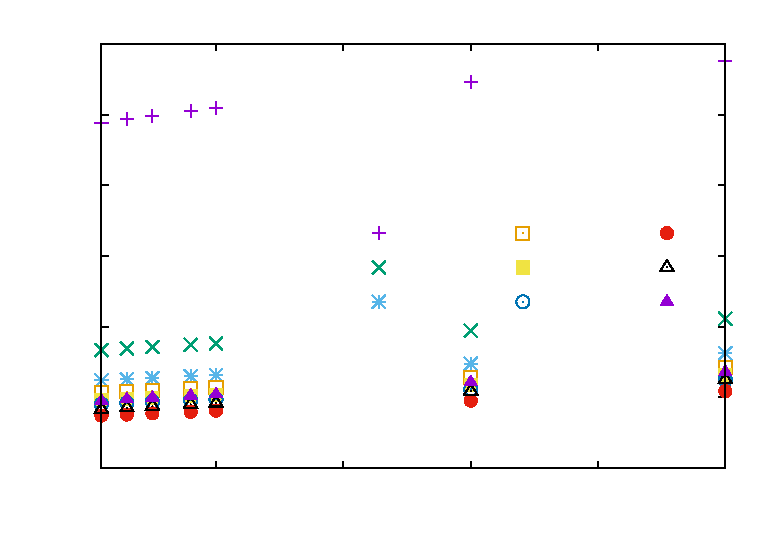
\includegraphics{../../Programming/sinking_bim_write_up/trunk/time_viscos}}%
    \gplfronttext
  \end{picture}%
\endgroup
}
        \caption{}
        \label{fig:time_viscos}
      \end{subfigure}
      ~
      \begin{subfigure}[b]{0.45\textwidth}
        \resizebox{\textwidth}{!}{\Large % GNUPLOT: LaTeX picture with Postscript
\begingroup
  \makeatletter
  \providecommand\color[2][]{%
    \GenericError{(gnuplot) \space\space\space\@spaces}{%
      Package color not loaded in conjunction with
      terminal option `colourtext'%
    }{See the gnuplot documentation for explanation.%
    }{Either use 'blacktext' in gnuplot or load the package
      color.sty in LaTeX.}%
    \renewcommand\color[2][]{}%
  }%
  \providecommand\includegraphics[2][]{%
    \GenericError{(gnuplot) \space\space\space\@spaces}{%
      Package graphicx or graphics not loaded%
    }{See the gnuplot documentation for explanation.%
    }{The gnuplot epslatex terminal needs graphicx.sty or graphics.sty.}%
    \renewcommand\includegraphics[2][]{}%
  }%
  \providecommand\rotatebox[2]{#2}%
  \@ifundefined{ifGPcolor}{%
    \newif\ifGPcolor
    \GPcolorfalse
  }{}%
  \@ifundefined{ifGPblacktext}{%
    \newif\ifGPblacktext
    \GPblacktexttrue
  }{}%
  % define a \g@addto@macro without @ in the name:
  \let\gplgaddtomacro\g@addto@macro
  % define empty templates for all commands taking text:
  \gdef\gplbacktext{}%
  \gdef\gplfronttext{}%
  \makeatother
  \ifGPblacktext
    % no textcolor at all
    \def\colorrgb#1{}%
    \def\colorgray#1{}%
  \else
    % gray or color?
    \ifGPcolor
      \def\colorrgb#1{\color[rgb]{#1}}%
      \def\colorgray#1{\color[gray]{#1}}%
      \expandafter\def\csname LTw\endcsname{\color{white}}%
      \expandafter\def\csname LTb\endcsname{\color{black}}%
      \expandafter\def\csname LTa\endcsname{\color{black}}%
      \expandafter\def\csname LT0\endcsname{\color[rgb]{1,0,0}}%
      \expandafter\def\csname LT1\endcsname{\color[rgb]{0,1,0}}%
      \expandafter\def\csname LT2\endcsname{\color[rgb]{0,0,1}}%
      \expandafter\def\csname LT3\endcsname{\color[rgb]{1,0,1}}%
      \expandafter\def\csname LT4\endcsname{\color[rgb]{0,1,1}}%
      \expandafter\def\csname LT5\endcsname{\color[rgb]{1,1,0}}%
      \expandafter\def\csname LT6\endcsname{\color[rgb]{0,0,0}}%
      \expandafter\def\csname LT7\endcsname{\color[rgb]{1,0.3,0}}%
      \expandafter\def\csname LT8\endcsname{\color[rgb]{0.5,0.5,0.5}}%
    \else
      % gray
      \def\colorrgb#1{\color{black}}%
      \def\colorgray#1{\color[gray]{#1}}%
      \expandafter\def\csname LTw\endcsname{\color{white}}%
      \expandafter\def\csname LTb\endcsname{\color{black}}%
      \expandafter\def\csname LTa\endcsname{\color{black}}%
      \expandafter\def\csname LT0\endcsname{\color{black}}%
      \expandafter\def\csname LT1\endcsname{\color{black}}%
      \expandafter\def\csname LT2\endcsname{\color{black}}%
      \expandafter\def\csname LT3\endcsname{\color{black}}%
      \expandafter\def\csname LT4\endcsname{\color{black}}%
      \expandafter\def\csname LT5\endcsname{\color{black}}%
      \expandafter\def\csname LT6\endcsname{\color{black}}%
      \expandafter\def\csname LT7\endcsname{\color{black}}%
      \expandafter\def\csname LT8\endcsname{\color{black}}%
    \fi
  \fi
    \setlength{\unitlength}{0.0500bp}%
    \ifx\gptboxheight\undefined%
      \newlength{\gptboxheight}%
      \newlength{\gptboxwidth}%
      \newsavebox{\gptboxtext}%
    \fi%
    \setlength{\fboxrule}{0.5pt}%
    \setlength{\fboxsep}{1pt}%
\begin{picture}(7200.00,5040.00)%
    \gplgaddtomacro\gplbacktext{%
      \csname LTb\endcsname%
      \put(682,704){\makebox(0,0)[r]{\strut{}$0$}}%
      \put(682,1383){\makebox(0,0)[r]{\strut{}$10$}}%
      \put(682,2061){\makebox(0,0)[r]{\strut{}$20$}}%
      \put(682,2740){\makebox(0,0)[r]{\strut{}$30$}}%
      \put(682,3418){\makebox(0,0)[r]{\strut{}$40$}}%
      \put(682,4097){\makebox(0,0)[r]{\strut{}$50$}}%
      \put(682,4775){\makebox(0,0)[r]{\strut{}$60$}}%
      \put(814,484){\makebox(0,0){\strut{}$0$}}%
      \put(1670,484){\makebox(0,0){\strut{}$1$}}%
      \put(2525,484){\makebox(0,0){\strut{}$2$}}%
      \put(3381,484){\makebox(0,0){\strut{}$3$}}%
      \put(4236,484){\makebox(0,0){\strut{}$4$}}%
      \put(5092,484){\makebox(0,0){\strut{}$5$}}%
      \put(5947,484){\makebox(0,0){\strut{}$6$}}%
      \put(6803,484){\makebox(0,0){\strut{}$7$}}%
    }%
    \gplgaddtomacro\gplfronttext{%
      \csname LTb\endcsname%
      \put(176,2739){\rotatebox{-270}{\makebox(0,0){\strut{}$t_{\text{s}}$}}}%
      \put(3808,154){\makebox(0,0){\strut{}$\ln D$}}%
      \put(5156,4547){\makebox(0,0){\strut{}$\lambda$}}%
      \csname LTb\endcsname%
      \put(4301,4327){\makebox(0,0)[r]{\strut{}0.001}}%
      \csname LTb\endcsname%
      \put(4301,3997){\makebox(0,0)[r]{\strut{}0.01}}%
      \csname LTb\endcsname%
      \put(5816,4327){\makebox(0,0)[r]{\strut{}0.03}}%
      \csname LTb\endcsname%
      \put(5816,3997){\makebox(0,0)[r]{\strut{}0.05}}%
    }%
    \gplbacktext
    \put(0,0){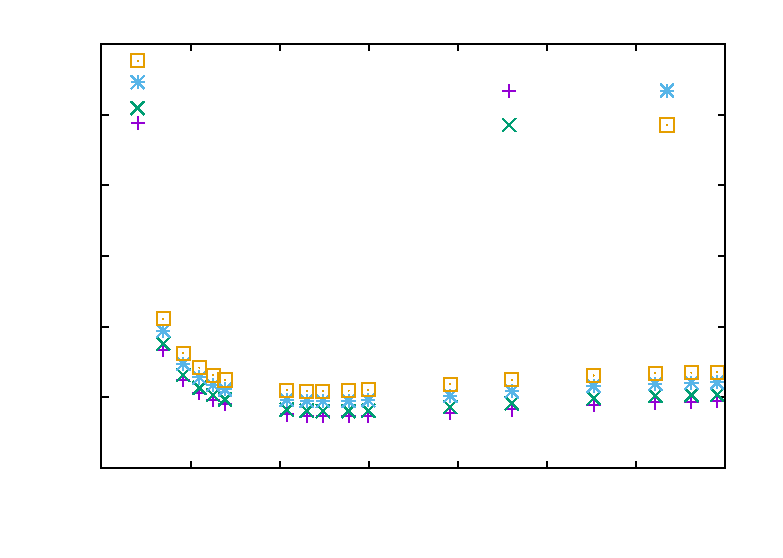
\includegraphics{../../Programming/sinking_bim_write_up/trunk/time_mdr}}%
    \gplfronttext
  \end{picture}%
\endgroup
}
        \caption{}
        \label{fig:time_mdr}
      \end{subfigure}
      \caption{Dependence of $t_{\text{s}}$ on a) $\lambda$ for different $D$ and b) $D$ for different $\lambda$, for $\Bo = 1000$, which is in the regime where $t_{\text{s}}$ is independent of $\Bo$.}\label{fig:highBo_time}
    \end{figure}

\subsection{Settling Spheroids}
\label{subsec:spheroids}

The settling of non-spherical particles shows different behaviour. Figure~\ref{fig:float_oblate} shows the settling of an oblate spheroid of aspect ratio $R = 0.5$ onto an interface, where the dimensionless parameters are $D = 2$, $\Bo = 10$ and $\lambda = 1$. As can be seen, the speroid is able to float at the interface. Comparing with figure~\ref{zoom_regime_pub.tex} it can be seen that for these values, spheres are observed to sink through the interface. Therefore, decreasing the aspect ratio of the particle can inhibit sinking. 

    \begin{figure}
      \centering
      \begin{subfigure}[b]{0.45\textwidth}
        \resizebox{\textwidth}{!}{\Large % GNUPLOT: LaTeX picture with Postscript
\begingroup
  \makeatletter
  \providecommand\color[2][]{%
    \GenericError{(gnuplot) \space\space\space\@spaces}{%
      Package color not loaded in conjunction with
      terminal option `colourtext'%
    }{See the gnuplot documentation for explanation.%
    }{Either use 'blacktext' in gnuplot or load the package
      color.sty in LaTeX.}%
    \renewcommand\color[2][]{}%
  }%
  \providecommand\includegraphics[2][]{%
    \GenericError{(gnuplot) \space\space\space\@spaces}{%
      Package graphicx or graphics not loaded%
    }{See the gnuplot documentation for explanation.%
    }{The gnuplot epslatex terminal needs graphicx.sty or graphics.sty.}%
    \renewcommand\includegraphics[2][]{}%
  }%
  \providecommand\rotatebox[2]{#2}%
  \@ifundefined{ifGPcolor}{%
    \newif\ifGPcolor
    \GPcolorfalse
  }{}%
  \@ifundefined{ifGPblacktext}{%
    \newif\ifGPblacktext
    \GPblacktexttrue
  }{}%
  % define a \g@addto@macro without @ in the name:
  \let\gplgaddtomacro\g@addto@macro
  % define empty templates for all commands taking text:
  \gdef\gplbacktext{}%
  \gdef\gplfronttext{}%
  \makeatother
  \ifGPblacktext
    % no textcolor at all
    \def\colorrgb#1{}%
    \def\colorgray#1{}%
  \else
    % gray or color?
    \ifGPcolor
      \def\colorrgb#1{\color[rgb]{#1}}%
      \def\colorgray#1{\color[gray]{#1}}%
      \expandafter\def\csname LTw\endcsname{\color{white}}%
      \expandafter\def\csname LTb\endcsname{\color{black}}%
      \expandafter\def\csname LTa\endcsname{\color{black}}%
      \expandafter\def\csname LT0\endcsname{\color[rgb]{1,0,0}}%
      \expandafter\def\csname LT1\endcsname{\color[rgb]{0,1,0}}%
      \expandafter\def\csname LT2\endcsname{\color[rgb]{0,0,1}}%
      \expandafter\def\csname LT3\endcsname{\color[rgb]{1,0,1}}%
      \expandafter\def\csname LT4\endcsname{\color[rgb]{0,1,1}}%
      \expandafter\def\csname LT5\endcsname{\color[rgb]{1,1,0}}%
      \expandafter\def\csname LT6\endcsname{\color[rgb]{0,0,0}}%
      \expandafter\def\csname LT7\endcsname{\color[rgb]{1,0.3,0}}%
      \expandafter\def\csname LT8\endcsname{\color[rgb]{0.5,0.5,0.5}}%
    \else
      % gray
      \def\colorrgb#1{\color{black}}%
      \def\colorgray#1{\color[gray]{#1}}%
      \expandafter\def\csname LTw\endcsname{\color{white}}%
      \expandafter\def\csname LTb\endcsname{\color{black}}%
      \expandafter\def\csname LTa\endcsname{\color{black}}%
      \expandafter\def\csname LT0\endcsname{\color{black}}%
      \expandafter\def\csname LT1\endcsname{\color{black}}%
      \expandafter\def\csname LT2\endcsname{\color{black}}%
      \expandafter\def\csname LT3\endcsname{\color{black}}%
      \expandafter\def\csname LT4\endcsname{\color{black}}%
      \expandafter\def\csname LT5\endcsname{\color{black}}%
      \expandafter\def\csname LT6\endcsname{\color{black}}%
      \expandafter\def\csname LT7\endcsname{\color{black}}%
      \expandafter\def\csname LT8\endcsname{\color{black}}%
    \fi
  \fi
    \setlength{\unitlength}{0.0500bp}%
    \ifx\gptboxheight\undefined%
      \newlength{\gptboxheight}%
      \newlength{\gptboxwidth}%
      \newsavebox{\gptboxtext}%
    \fi%
    \setlength{\fboxrule}{0.5pt}%
    \setlength{\fboxsep}{1pt}%
\begin{picture}(7200.00,5040.00)%
    \gplgaddtomacro\gplbacktext{%
      \csname LTb\endcsname%
      \put(1597,440){\makebox(0,0)[r]{\strut{}$-6$}}%
      \put(1597,1097){\makebox(0,0)[r]{\strut{}$-4$}}%
      \put(1597,1753){\makebox(0,0)[r]{\strut{}$-2$}}%
      \put(1597,2410){\makebox(0,0)[r]{\strut{}$0$}}%
      \put(1597,3066){\makebox(0,0)[r]{\strut{}$2$}}%
      \put(1597,3723){\makebox(0,0)[r]{\strut{}$4$}}%
      \put(1597,4379){\makebox(0,0)[r]{\strut{}$6$}}%
      \put(1729,220){\makebox(0,0){\strut{}$-6$}}%
      \put(2386,220){\makebox(0,0){\strut{}$-4$}}%
      \put(3042,220){\makebox(0,0){\strut{}$-2$}}%
      \put(3699,220){\makebox(0,0){\strut{}$0$}}%
      \put(4355,220){\makebox(0,0){\strut{}$2$}}%
      \put(5012,220){\makebox(0,0){\strut{}$4$}}%
      \put(5668,220){\makebox(0,0){\strut{}$6$}}%
    }%
    \gplgaddtomacro\gplfronttext{%
      \csname LTb\endcsname%
      \put(3698,4709){\makebox(0,0){\strut{}$t = 0$}}%
    }%
    \gplbacktext
    \put(0,0){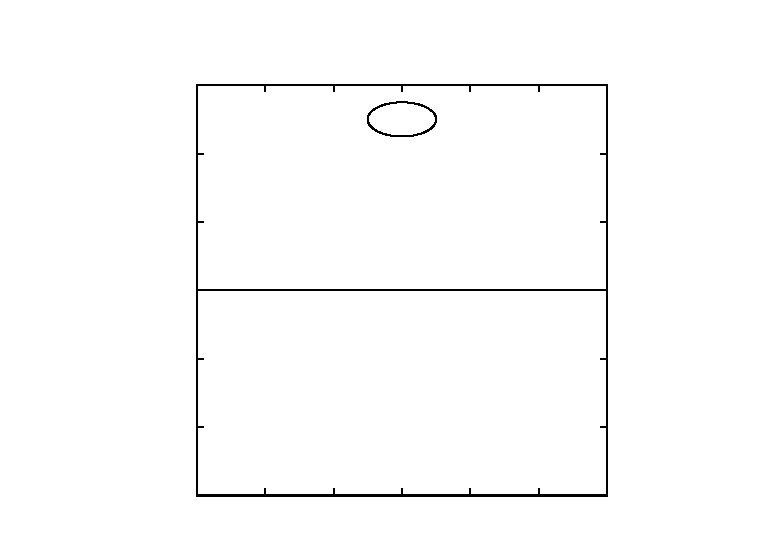
\includegraphics{../../Programming/sinking_bim_write_up/trunk/ob_float1}}%
    \gplfronttext
  \end{picture}%
\endgroup
}
        \caption{}
        \label{fig:ob_float1}
      \end{subfigure}
      ~
      \begin{subfigure}[b]{0.45\textwidth}
        \resizebox{\textwidth}{!}{\Large % GNUPLOT: LaTeX picture with Postscript
\begingroup
  \makeatletter
  \providecommand\color[2][]{%
    \GenericError{(gnuplot) \space\space\space\@spaces}{%
      Package color not loaded in conjunction with
      terminal option `colourtext'%
    }{See the gnuplot documentation for explanation.%
    }{Either use 'blacktext' in gnuplot or load the package
      color.sty in LaTeX.}%
    \renewcommand\color[2][]{}%
  }%
  \providecommand\includegraphics[2][]{%
    \GenericError{(gnuplot) \space\space\space\@spaces}{%
      Package graphicx or graphics not loaded%
    }{See the gnuplot documentation for explanation.%
    }{The gnuplot epslatex terminal needs graphicx.sty or graphics.sty.}%
    \renewcommand\includegraphics[2][]{}%
  }%
  \providecommand\rotatebox[2]{#2}%
  \@ifundefined{ifGPcolor}{%
    \newif\ifGPcolor
    \GPcolorfalse
  }{}%
  \@ifundefined{ifGPblacktext}{%
    \newif\ifGPblacktext
    \GPblacktexttrue
  }{}%
  % define a \g@addto@macro without @ in the name:
  \let\gplgaddtomacro\g@addto@macro
  % define empty templates for all commands taking text:
  \gdef\gplbacktext{}%
  \gdef\gplfronttext{}%
  \makeatother
  \ifGPblacktext
    % no textcolor at all
    \def\colorrgb#1{}%
    \def\colorgray#1{}%
  \else
    % gray or color?
    \ifGPcolor
      \def\colorrgb#1{\color[rgb]{#1}}%
      \def\colorgray#1{\color[gray]{#1}}%
      \expandafter\def\csname LTw\endcsname{\color{white}}%
      \expandafter\def\csname LTb\endcsname{\color{black}}%
      \expandafter\def\csname LTa\endcsname{\color{black}}%
      \expandafter\def\csname LT0\endcsname{\color[rgb]{1,0,0}}%
      \expandafter\def\csname LT1\endcsname{\color[rgb]{0,1,0}}%
      \expandafter\def\csname LT2\endcsname{\color[rgb]{0,0,1}}%
      \expandafter\def\csname LT3\endcsname{\color[rgb]{1,0,1}}%
      \expandafter\def\csname LT4\endcsname{\color[rgb]{0,1,1}}%
      \expandafter\def\csname LT5\endcsname{\color[rgb]{1,1,0}}%
      \expandafter\def\csname LT6\endcsname{\color[rgb]{0,0,0}}%
      \expandafter\def\csname LT7\endcsname{\color[rgb]{1,0.3,0}}%
      \expandafter\def\csname LT8\endcsname{\color[rgb]{0.5,0.5,0.5}}%
    \else
      % gray
      \def\colorrgb#1{\color{black}}%
      \def\colorgray#1{\color[gray]{#1}}%
      \expandafter\def\csname LTw\endcsname{\color{white}}%
      \expandafter\def\csname LTb\endcsname{\color{black}}%
      \expandafter\def\csname LTa\endcsname{\color{black}}%
      \expandafter\def\csname LT0\endcsname{\color{black}}%
      \expandafter\def\csname LT1\endcsname{\color{black}}%
      \expandafter\def\csname LT2\endcsname{\color{black}}%
      \expandafter\def\csname LT3\endcsname{\color{black}}%
      \expandafter\def\csname LT4\endcsname{\color{black}}%
      \expandafter\def\csname LT5\endcsname{\color{black}}%
      \expandafter\def\csname LT6\endcsname{\color{black}}%
      \expandafter\def\csname LT7\endcsname{\color{black}}%
      \expandafter\def\csname LT8\endcsname{\color{black}}%
    \fi
  \fi
    \setlength{\unitlength}{0.0500bp}%
    \ifx\gptboxheight\undefined%
      \newlength{\gptboxheight}%
      \newlength{\gptboxwidth}%
      \newsavebox{\gptboxtext}%
    \fi%
    \setlength{\fboxrule}{0.5pt}%
    \setlength{\fboxsep}{1pt}%
\begin{picture}(7200.00,5040.00)%
    \gplgaddtomacro\gplbacktext{%
      \csname LTb\endcsname%
      \put(1597,440){\makebox(0,0)[r]{\strut{}$-6$}}%
      \put(1597,1097){\makebox(0,0)[r]{\strut{}$-4$}}%
      \put(1597,1753){\makebox(0,0)[r]{\strut{}$-2$}}%
      \put(1597,2410){\makebox(0,0)[r]{\strut{}$0$}}%
      \put(1597,3066){\makebox(0,0)[r]{\strut{}$2$}}%
      \put(1597,3723){\makebox(0,0)[r]{\strut{}$4$}}%
      \put(1597,4379){\makebox(0,0)[r]{\strut{}$6$}}%
      \put(1729,220){\makebox(0,0){\strut{}$-6$}}%
      \put(2386,220){\makebox(0,0){\strut{}$-4$}}%
      \put(3042,220){\makebox(0,0){\strut{}$-2$}}%
      \put(3699,220){\makebox(0,0){\strut{}$0$}}%
      \put(4355,220){\makebox(0,0){\strut{}$2$}}%
      \put(5012,220){\makebox(0,0){\strut{}$4$}}%
      \put(5668,220){\makebox(0,0){\strut{}$6$}}%
    }%
    \gplgaddtomacro\gplfronttext{%
      \csname LTb\endcsname%
      \put(3698,4709){\makebox(0,0){\strut{}$t = 2.52$}}%
    }%
    \gplbacktext
    \put(0,0){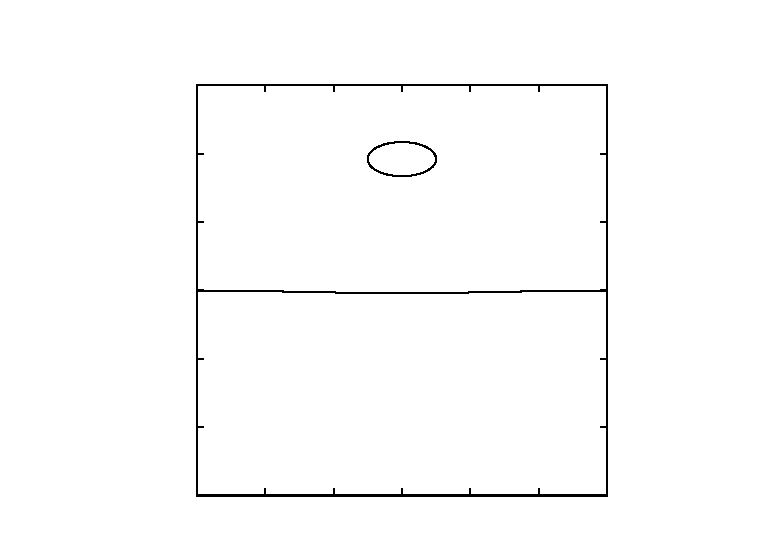
\includegraphics{../../Programming/sinking_bim_write_up/trunk/ob_float2}}%
    \gplfronttext
  \end{picture}%
\endgroup
}
        \caption{}
        \label{fig:ob_float2}
      \end{subfigure}
      
      \begin{subfigure}[b]{0.45\textwidth}
        \resizebox{\textwidth}{!}{\Large % GNUPLOT: LaTeX picture with Postscript
\begingroup
  \makeatletter
  \providecommand\color[2][]{%
    \GenericError{(gnuplot) \space\space\space\@spaces}{%
      Package color not loaded in conjunction with
      terminal option `colourtext'%
    }{See the gnuplot documentation for explanation.%
    }{Either use 'blacktext' in gnuplot or load the package
      color.sty in LaTeX.}%
    \renewcommand\color[2][]{}%
  }%
  \providecommand\includegraphics[2][]{%
    \GenericError{(gnuplot) \space\space\space\@spaces}{%
      Package graphicx or graphics not loaded%
    }{See the gnuplot documentation for explanation.%
    }{The gnuplot epslatex terminal needs graphicx.sty or graphics.sty.}%
    \renewcommand\includegraphics[2][]{}%
  }%
  \providecommand\rotatebox[2]{#2}%
  \@ifundefined{ifGPcolor}{%
    \newif\ifGPcolor
    \GPcolorfalse
  }{}%
  \@ifundefined{ifGPblacktext}{%
    \newif\ifGPblacktext
    \GPblacktexttrue
  }{}%
  % define a \g@addto@macro without @ in the name:
  \let\gplgaddtomacro\g@addto@macro
  % define empty templates for all commands taking text:
  \gdef\gplbacktext{}%
  \gdef\gplfronttext{}%
  \makeatother
  \ifGPblacktext
    % no textcolor at all
    \def\colorrgb#1{}%
    \def\colorgray#1{}%
  \else
    % gray or color?
    \ifGPcolor
      \def\colorrgb#1{\color[rgb]{#1}}%
      \def\colorgray#1{\color[gray]{#1}}%
      \expandafter\def\csname LTw\endcsname{\color{white}}%
      \expandafter\def\csname LTb\endcsname{\color{black}}%
      \expandafter\def\csname LTa\endcsname{\color{black}}%
      \expandafter\def\csname LT0\endcsname{\color[rgb]{1,0,0}}%
      \expandafter\def\csname LT1\endcsname{\color[rgb]{0,1,0}}%
      \expandafter\def\csname LT2\endcsname{\color[rgb]{0,0,1}}%
      \expandafter\def\csname LT3\endcsname{\color[rgb]{1,0,1}}%
      \expandafter\def\csname LT4\endcsname{\color[rgb]{0,1,1}}%
      \expandafter\def\csname LT5\endcsname{\color[rgb]{1,1,0}}%
      \expandafter\def\csname LT6\endcsname{\color[rgb]{0,0,0}}%
      \expandafter\def\csname LT7\endcsname{\color[rgb]{1,0.3,0}}%
      \expandafter\def\csname LT8\endcsname{\color[rgb]{0.5,0.5,0.5}}%
    \else
      % gray
      \def\colorrgb#1{\color{black}}%
      \def\colorgray#1{\color[gray]{#1}}%
      \expandafter\def\csname LTw\endcsname{\color{white}}%
      \expandafter\def\csname LTb\endcsname{\color{black}}%
      \expandafter\def\csname LTa\endcsname{\color{black}}%
      \expandafter\def\csname LT0\endcsname{\color{black}}%
      \expandafter\def\csname LT1\endcsname{\color{black}}%
      \expandafter\def\csname LT2\endcsname{\color{black}}%
      \expandafter\def\csname LT3\endcsname{\color{black}}%
      \expandafter\def\csname LT4\endcsname{\color{black}}%
      \expandafter\def\csname LT5\endcsname{\color{black}}%
      \expandafter\def\csname LT6\endcsname{\color{black}}%
      \expandafter\def\csname LT7\endcsname{\color{black}}%
      \expandafter\def\csname LT8\endcsname{\color{black}}%
    \fi
  \fi
    \setlength{\unitlength}{0.0500bp}%
    \ifx\gptboxheight\undefined%
      \newlength{\gptboxheight}%
      \newlength{\gptboxwidth}%
      \newsavebox{\gptboxtext}%
    \fi%
    \setlength{\fboxrule}{0.5pt}%
    \setlength{\fboxsep}{1pt}%
\begin{picture}(7200.00,5040.00)%
    \gplgaddtomacro\gplbacktext{%
      \csname LTb\endcsname%
      \put(1597,440){\makebox(0,0)[r]{\strut{}$-6$}}%
      \put(1597,1097){\makebox(0,0)[r]{\strut{}$-4$}}%
      \put(1597,1753){\makebox(0,0)[r]{\strut{}$-2$}}%
      \put(1597,2410){\makebox(0,0)[r]{\strut{}$0$}}%
      \put(1597,3066){\makebox(0,0)[r]{\strut{}$2$}}%
      \put(1597,3723){\makebox(0,0)[r]{\strut{}$4$}}%
      \put(1597,4379){\makebox(0,0)[r]{\strut{}$6$}}%
      \put(1729,220){\makebox(0,0){\strut{}$-6$}}%
      \put(2386,220){\makebox(0,0){\strut{}$-4$}}%
      \put(3042,220){\makebox(0,0){\strut{}$-2$}}%
      \put(3699,220){\makebox(0,0){\strut{}$0$}}%
      \put(4355,220){\makebox(0,0){\strut{}$2$}}%
      \put(5012,220){\makebox(0,0){\strut{}$4$}}%
      \put(5668,220){\makebox(0,0){\strut{}$6$}}%
    }%
    \gplgaddtomacro\gplfronttext{%
      \csname LTb\endcsname%
      \put(3698,4709){\makebox(0,0){\strut{}$t = 4.46$}}%
    }%
    \gplbacktext
    \put(0,0){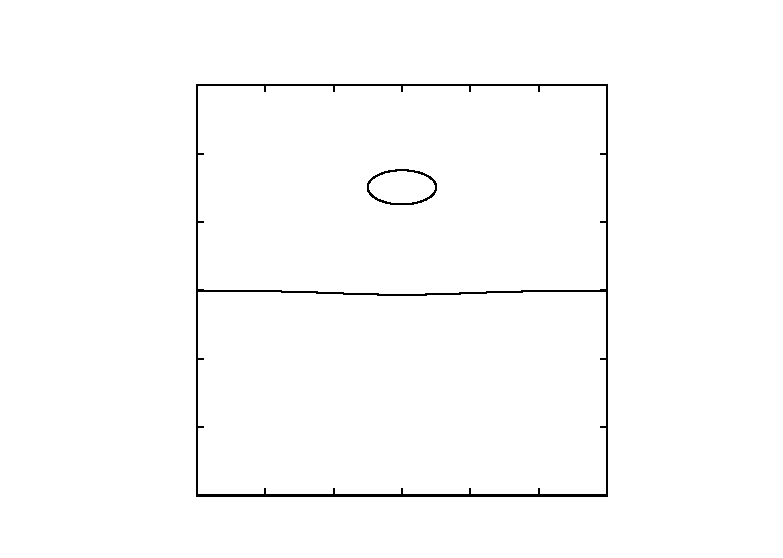
\includegraphics{../../Programming/sinking_bim_write_up/trunk/ob_float3}}%
    \gplfronttext
  \end{picture}%
\endgroup
}
        \caption{}
        \label{fig:ob_float3}
      \end{subfigure}
      ~
      \begin{subfigure}[b]{0.45\textwidth}
        \resizebox{\textwidth}{!}{\Large % GNUPLOT: LaTeX picture with Postscript
\begingroup
  \makeatletter
  \providecommand\color[2][]{%
    \GenericError{(gnuplot) \space\space\space\@spaces}{%
      Package color not loaded in conjunction with
      terminal option `colourtext'%
    }{See the gnuplot documentation for explanation.%
    }{Either use 'blacktext' in gnuplot or load the package
      color.sty in LaTeX.}%
    \renewcommand\color[2][]{}%
  }%
  \providecommand\includegraphics[2][]{%
    \GenericError{(gnuplot) \space\space\space\@spaces}{%
      Package graphicx or graphics not loaded%
    }{See the gnuplot documentation for explanation.%
    }{The gnuplot epslatex terminal needs graphicx.sty or graphics.sty.}%
    \renewcommand\includegraphics[2][]{}%
  }%
  \providecommand\rotatebox[2]{#2}%
  \@ifundefined{ifGPcolor}{%
    \newif\ifGPcolor
    \GPcolorfalse
  }{}%
  \@ifundefined{ifGPblacktext}{%
    \newif\ifGPblacktext
    \GPblacktexttrue
  }{}%
  % define a \g@addto@macro without @ in the name:
  \let\gplgaddtomacro\g@addto@macro
  % define empty templates for all commands taking text:
  \gdef\gplbacktext{}%
  \gdef\gplfronttext{}%
  \makeatother
  \ifGPblacktext
    % no textcolor at all
    \def\colorrgb#1{}%
    \def\colorgray#1{}%
  \else
    % gray or color?
    \ifGPcolor
      \def\colorrgb#1{\color[rgb]{#1}}%
      \def\colorgray#1{\color[gray]{#1}}%
      \expandafter\def\csname LTw\endcsname{\color{white}}%
      \expandafter\def\csname LTb\endcsname{\color{black}}%
      \expandafter\def\csname LTa\endcsname{\color{black}}%
      \expandafter\def\csname LT0\endcsname{\color[rgb]{1,0,0}}%
      \expandafter\def\csname LT1\endcsname{\color[rgb]{0,1,0}}%
      \expandafter\def\csname LT2\endcsname{\color[rgb]{0,0,1}}%
      \expandafter\def\csname LT3\endcsname{\color[rgb]{1,0,1}}%
      \expandafter\def\csname LT4\endcsname{\color[rgb]{0,1,1}}%
      \expandafter\def\csname LT5\endcsname{\color[rgb]{1,1,0}}%
      \expandafter\def\csname LT6\endcsname{\color[rgb]{0,0,0}}%
      \expandafter\def\csname LT7\endcsname{\color[rgb]{1,0.3,0}}%
      \expandafter\def\csname LT8\endcsname{\color[rgb]{0.5,0.5,0.5}}%
    \else
      % gray
      \def\colorrgb#1{\color{black}}%
      \def\colorgray#1{\color[gray]{#1}}%
      \expandafter\def\csname LTw\endcsname{\color{white}}%
      \expandafter\def\csname LTb\endcsname{\color{black}}%
      \expandafter\def\csname LTa\endcsname{\color{black}}%
      \expandafter\def\csname LT0\endcsname{\color{black}}%
      \expandafter\def\csname LT1\endcsname{\color{black}}%
      \expandafter\def\csname LT2\endcsname{\color{black}}%
      \expandafter\def\csname LT3\endcsname{\color{black}}%
      \expandafter\def\csname LT4\endcsname{\color{black}}%
      \expandafter\def\csname LT5\endcsname{\color{black}}%
      \expandafter\def\csname LT6\endcsname{\color{black}}%
      \expandafter\def\csname LT7\endcsname{\color{black}}%
      \expandafter\def\csname LT8\endcsname{\color{black}}%
    \fi
  \fi
    \setlength{\unitlength}{0.0500bp}%
    \ifx\gptboxheight\undefined%
      \newlength{\gptboxheight}%
      \newlength{\gptboxwidth}%
      \newsavebox{\gptboxtext}%
    \fi%
    \setlength{\fboxrule}{0.5pt}%
    \setlength{\fboxsep}{1pt}%
\begin{picture}(7200.00,5040.00)%
    \gplgaddtomacro\gplbacktext{%
      \csname LTb\endcsname%
      \put(1597,440){\makebox(0,0)[r]{\strut{}$-6$}}%
      \put(1597,1097){\makebox(0,0)[r]{\strut{}$-4$}}%
      \put(1597,1753){\makebox(0,0)[r]{\strut{}$-2$}}%
      \put(1597,2410){\makebox(0,0)[r]{\strut{}$0$}}%
      \put(1597,3066){\makebox(0,0)[r]{\strut{}$2$}}%
      \put(1597,3723){\makebox(0,0)[r]{\strut{}$4$}}%
      \put(1597,4379){\makebox(0,0)[r]{\strut{}$6$}}%
      \put(1729,220){\makebox(0,0){\strut{}$-6$}}%
      \put(2386,220){\makebox(0,0){\strut{}$-4$}}%
      \put(3042,220){\makebox(0,0){\strut{}$-2$}}%
      \put(3699,220){\makebox(0,0){\strut{}$0$}}%
      \put(4355,220){\makebox(0,0){\strut{}$2$}}%
      \put(5012,220){\makebox(0,0){\strut{}$4$}}%
      \put(5668,220){\makebox(0,0){\strut{}$6$}}%
    }%
    \gplgaddtomacro\gplfronttext{%
      \csname LTb\endcsname%
      \put(3698,4709){\makebox(0,0){\strut{}$t = 7.02$}}%
    }%
    \gplbacktext
    \put(0,0){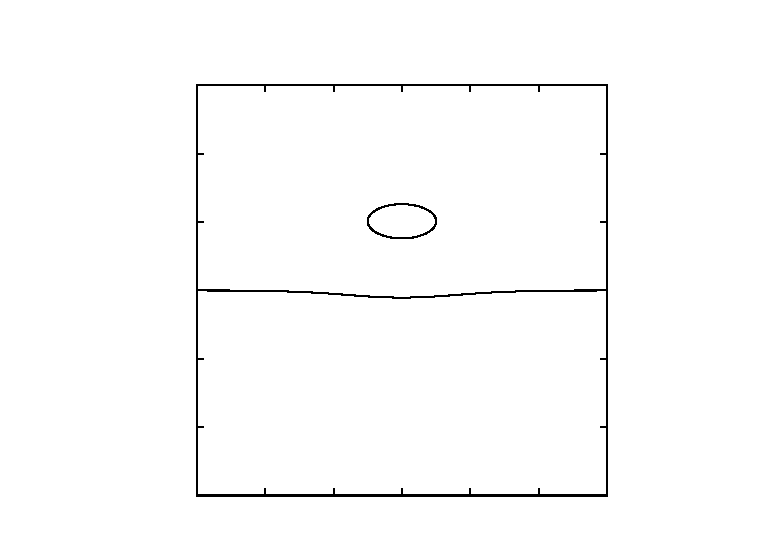
\includegraphics{../../Programming/sinking_bim_write_up/trunk/ob_float4}}%
    \gplfronttext
  \end{picture}%
\endgroup
}
        \caption{}
        \label{fig:ob_float4}
      \end{subfigure}
      
      \begin{subfigure}[b]{0.45\textwidth}
        \resizebox{\textwidth}{!}{\Large % GNUPLOT: LaTeX picture with Postscript
\begingroup
  \makeatletter
  \providecommand\color[2][]{%
    \GenericError{(gnuplot) \space\space\space\@spaces}{%
      Package color not loaded in conjunction with
      terminal option `colourtext'%
    }{See the gnuplot documentation for explanation.%
    }{Either use 'blacktext' in gnuplot or load the package
      color.sty in LaTeX.}%
    \renewcommand\color[2][]{}%
  }%
  \providecommand\includegraphics[2][]{%
    \GenericError{(gnuplot) \space\space\space\@spaces}{%
      Package graphicx or graphics not loaded%
    }{See the gnuplot documentation for explanation.%
    }{The gnuplot epslatex terminal needs graphicx.sty or graphics.sty.}%
    \renewcommand\includegraphics[2][]{}%
  }%
  \providecommand\rotatebox[2]{#2}%
  \@ifundefined{ifGPcolor}{%
    \newif\ifGPcolor
    \GPcolorfalse
  }{}%
  \@ifundefined{ifGPblacktext}{%
    \newif\ifGPblacktext
    \GPblacktexttrue
  }{}%
  % define a \g@addto@macro without @ in the name:
  \let\gplgaddtomacro\g@addto@macro
  % define empty templates for all commands taking text:
  \gdef\gplbacktext{}%
  \gdef\gplfronttext{}%
  \makeatother
  \ifGPblacktext
    % no textcolor at all
    \def\colorrgb#1{}%
    \def\colorgray#1{}%
  \else
    % gray or color?
    \ifGPcolor
      \def\colorrgb#1{\color[rgb]{#1}}%
      \def\colorgray#1{\color[gray]{#1}}%
      \expandafter\def\csname LTw\endcsname{\color{white}}%
      \expandafter\def\csname LTb\endcsname{\color{black}}%
      \expandafter\def\csname LTa\endcsname{\color{black}}%
      \expandafter\def\csname LT0\endcsname{\color[rgb]{1,0,0}}%
      \expandafter\def\csname LT1\endcsname{\color[rgb]{0,1,0}}%
      \expandafter\def\csname LT2\endcsname{\color[rgb]{0,0,1}}%
      \expandafter\def\csname LT3\endcsname{\color[rgb]{1,0,1}}%
      \expandafter\def\csname LT4\endcsname{\color[rgb]{0,1,1}}%
      \expandafter\def\csname LT5\endcsname{\color[rgb]{1,1,0}}%
      \expandafter\def\csname LT6\endcsname{\color[rgb]{0,0,0}}%
      \expandafter\def\csname LT7\endcsname{\color[rgb]{1,0.3,0}}%
      \expandafter\def\csname LT8\endcsname{\color[rgb]{0.5,0.5,0.5}}%
    \else
      % gray
      \def\colorrgb#1{\color{black}}%
      \def\colorgray#1{\color[gray]{#1}}%
      \expandafter\def\csname LTw\endcsname{\color{white}}%
      \expandafter\def\csname LTb\endcsname{\color{black}}%
      \expandafter\def\csname LTa\endcsname{\color{black}}%
      \expandafter\def\csname LT0\endcsname{\color{black}}%
      \expandafter\def\csname LT1\endcsname{\color{black}}%
      \expandafter\def\csname LT2\endcsname{\color{black}}%
      \expandafter\def\csname LT3\endcsname{\color{black}}%
      \expandafter\def\csname LT4\endcsname{\color{black}}%
      \expandafter\def\csname LT5\endcsname{\color{black}}%
      \expandafter\def\csname LT6\endcsname{\color{black}}%
      \expandafter\def\csname LT7\endcsname{\color{black}}%
      \expandafter\def\csname LT8\endcsname{\color{black}}%
    \fi
  \fi
    \setlength{\unitlength}{0.0500bp}%
    \ifx\gptboxheight\undefined%
      \newlength{\gptboxheight}%
      \newlength{\gptboxwidth}%
      \newsavebox{\gptboxtext}%
    \fi%
    \setlength{\fboxrule}{0.5pt}%
    \setlength{\fboxsep}{1pt}%
\begin{picture}(7200.00,5040.00)%
    \gplgaddtomacro\gplbacktext{%
      \csname LTb\endcsname%
      \put(1597,440){\makebox(0,0)[r]{\strut{}$-6$}}%
      \put(1597,1097){\makebox(0,0)[r]{\strut{}$-4$}}%
      \put(1597,1753){\makebox(0,0)[r]{\strut{}$-2$}}%
      \put(1597,2410){\makebox(0,0)[r]{\strut{}$0$}}%
      \put(1597,3066){\makebox(0,0)[r]{\strut{}$2$}}%
      \put(1597,3723){\makebox(0,0)[r]{\strut{}$4$}}%
      \put(1597,4379){\makebox(0,0)[r]{\strut{}$6$}}%
      \put(1729,220){\makebox(0,0){\strut{}$-6$}}%
      \put(2386,220){\makebox(0,0){\strut{}$-4$}}%
      \put(3042,220){\makebox(0,0){\strut{}$-2$}}%
      \put(3699,220){\makebox(0,0){\strut{}$0$}}%
      \put(4355,220){\makebox(0,0){\strut{}$2$}}%
      \put(5012,220){\makebox(0,0){\strut{}$4$}}%
      \put(5668,220){\makebox(0,0){\strut{}$6$}}%
    }%
    \gplgaddtomacro\gplfronttext{%
      \csname LTb\endcsname%
      \put(3698,4709){\makebox(0,0){\strut{}$t = 10.17$}}%
    }%
    \gplbacktext
    \put(0,0){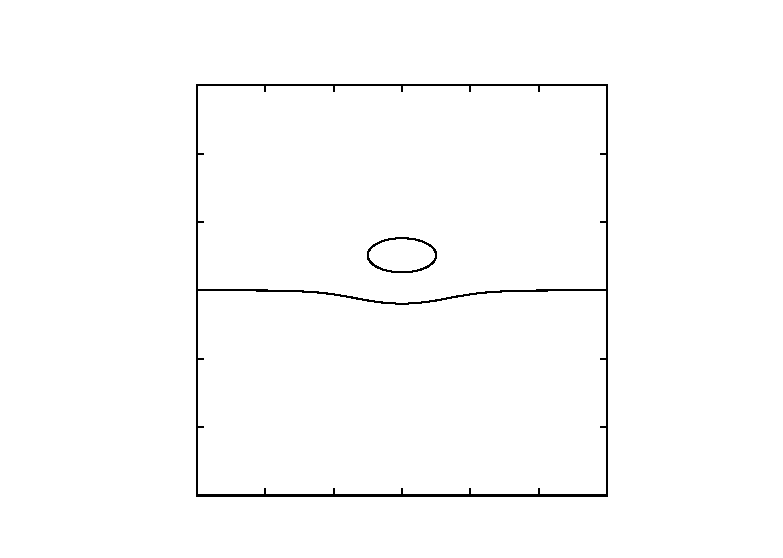
\includegraphics{../../Programming/sinking_bim_write_up/trunk/ob_float5}}%
    \gplfronttext
  \end{picture}%
\endgroup
}
        \caption{}
        \label{fig:ob_float5}
      \end{subfigure}
      ~
      \begin{subfigure}[b]{0.45\textwidth}
        \resizebox{\textwidth}{!}{\large % GNUPLOT: LaTeX picture with Postscript
\begingroup
  \makeatletter
  \providecommand\color[2][]{%
    \GenericError{(gnuplot) \space\space\space\@spaces}{%
      Package color not loaded in conjunction with
      terminal option `colourtext'%
    }{See the gnuplot documentation for explanation.%
    }{Either use 'blacktext' in gnuplot or load the package
      color.sty in LaTeX.}%
    \renewcommand\color[2][]{}%
  }%
  \providecommand\includegraphics[2][]{%
    \GenericError{(gnuplot) \space\space\space\@spaces}{%
      Package graphicx or graphics not loaded%
    }{See the gnuplot documentation for explanation.%
    }{The gnuplot epslatex terminal needs graphicx.sty or graphics.sty.}%
    \renewcommand\includegraphics[2][]{}%
  }%
  \providecommand\rotatebox[2]{#2}%
  \@ifundefined{ifGPcolor}{%
    \newif\ifGPcolor
    \GPcolorfalse
  }{}%
  \@ifundefined{ifGPblacktext}{%
    \newif\ifGPblacktext
    \GPblacktexttrue
  }{}%
  % define a \g@addto@macro without @ in the name:
  \let\gplgaddtomacro\g@addto@macro
  % define empty templates for all commands taking text:
  \gdef\gplbacktext{}%
  \gdef\gplfronttext{}%
  \makeatother
  \ifGPblacktext
    % no textcolor at all
    \def\colorrgb#1{}%
    \def\colorgray#1{}%
  \else
    % gray or color?
    \ifGPcolor
      \def\colorrgb#1{\color[rgb]{#1}}%
      \def\colorgray#1{\color[gray]{#1}}%
      \expandafter\def\csname LTw\endcsname{\color{white}}%
      \expandafter\def\csname LTb\endcsname{\color{black}}%
      \expandafter\def\csname LTa\endcsname{\color{black}}%
      \expandafter\def\csname LT0\endcsname{\color[rgb]{1,0,0}}%
      \expandafter\def\csname LT1\endcsname{\color[rgb]{0,1,0}}%
      \expandafter\def\csname LT2\endcsname{\color[rgb]{0,0,1}}%
      \expandafter\def\csname LT3\endcsname{\color[rgb]{1,0,1}}%
      \expandafter\def\csname LT4\endcsname{\color[rgb]{0,1,1}}%
      \expandafter\def\csname LT5\endcsname{\color[rgb]{1,1,0}}%
      \expandafter\def\csname LT6\endcsname{\color[rgb]{0,0,0}}%
      \expandafter\def\csname LT7\endcsname{\color[rgb]{1,0.3,0}}%
      \expandafter\def\csname LT8\endcsname{\color[rgb]{0.5,0.5,0.5}}%
    \else
      % gray
      \def\colorrgb#1{\color{black}}%
      \def\colorgray#1{\color[gray]{#1}}%
      \expandafter\def\csname LTw\endcsname{\color{white}}%
      \expandafter\def\csname LTb\endcsname{\color{black}}%
      \expandafter\def\csname LTa\endcsname{\color{black}}%
      \expandafter\def\csname LT0\endcsname{\color{black}}%
      \expandafter\def\csname LT1\endcsname{\color{black}}%
      \expandafter\def\csname LT2\endcsname{\color{black}}%
      \expandafter\def\csname LT3\endcsname{\color{black}}%
      \expandafter\def\csname LT4\endcsname{\color{black}}%
      \expandafter\def\csname LT5\endcsname{\color{black}}%
      \expandafter\def\csname LT6\endcsname{\color{black}}%
      \expandafter\def\csname LT7\endcsname{\color{black}}%
      \expandafter\def\csname LT8\endcsname{\color{black}}%
    \fi
  \fi
    \setlength{\unitlength}{0.0500bp}%
    \ifx\gptboxheight\undefined%
      \newlength{\gptboxheight}%
      \newlength{\gptboxwidth}%
      \newsavebox{\gptboxtext}%
    \fi%
    \setlength{\fboxrule}{0.5pt}%
    \setlength{\fboxsep}{1pt}%
\begin{picture}(7200.00,5040.00)%
    \gplgaddtomacro\gplbacktext{%
      \csname LTb\endcsname%
      \put(1597,440){\makebox(0,0)[r]{\strut{}$-6$}}%
      \put(1597,1097){\makebox(0,0)[r]{\strut{}$-4$}}%
      \put(1597,1753){\makebox(0,0)[r]{\strut{}$-2$}}%
      \put(1597,2410){\makebox(0,0)[r]{\strut{}$0$}}%
      \put(1597,3066){\makebox(0,0)[r]{\strut{}$2$}}%
      \put(1597,3723){\makebox(0,0)[r]{\strut{}$4$}}%
      \put(1597,4379){\makebox(0,0)[r]{\strut{}$6$}}%
      \put(1729,220){\makebox(0,0){\strut{}$-6$}}%
      \put(2386,220){\makebox(0,0){\strut{}$-4$}}%
      \put(3042,220){\makebox(0,0){\strut{}$-2$}}%
      \put(3699,220){\makebox(0,0){\strut{}$0$}}%
      \put(4355,220){\makebox(0,0){\strut{}$2$}}%
      \put(5012,220){\makebox(0,0){\strut{}$4$}}%
      \put(5668,220){\makebox(0,0){\strut{}$6$}}%
    }%
    \gplgaddtomacro\gplfronttext{%
      \csname LTb\endcsname%
      \put(3698,4709){\makebox(0,0){\strut{}$t = 999.99$}}%
    }%
    \gplbacktext
    \put(0,0){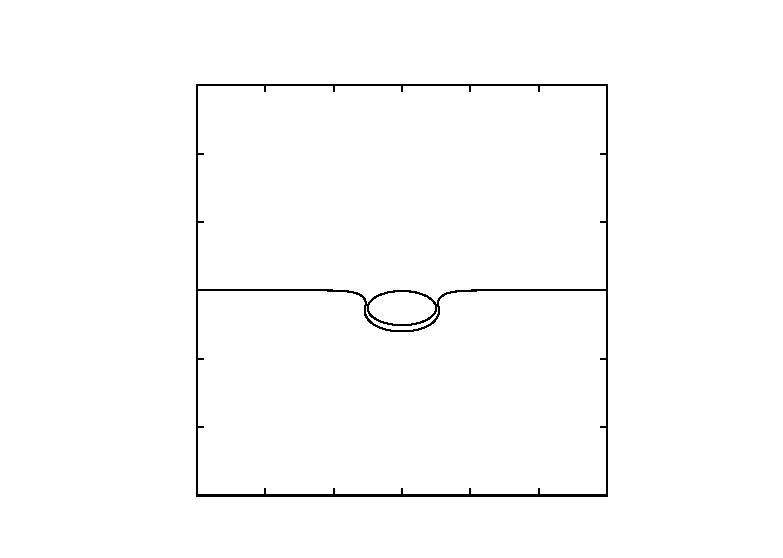
\includegraphics{../../Programming/sinking_bim_write_up/trunk/ob_float6}}%
    \gplfronttext
  \end{picture}%
\endgroup
}
        \caption{}
        \label{fig:ob_float6}
      \end{subfigure}
      \caption{Settling of an oblate spheroid with aspect ratio $R = 0.5$ onto the interface when $D = 2$, $\Bo = 10$ and $\lambda = 1$. The interface deforms as the sphere approaches and forms a depression into which the spheroid sits. }\label{fig:float_oblate}
    \end{figure}

Figure~\ref{fig:sinking_comp} compares the sinking of a sphere and that of a spheroid of aspect ratio $0.5$ where $D = \Bo = 1000$ and $\lambda = 1$. It is seen that at a given depth, the interfacial profile in both simulations is very similar, although it takes the spheroid much longer for it to reach that depth. In all simulations of an oblate spheroid where sinking was observed, all models terminated due to the separation between particle and interface becoming smaller than the distance between discretisation points. Hence, no simulations proceeded to tail snapping and therefore no data has been obtained regarding the sinking timescale and the entrained volume.
    \begin{figure}
      \centering
      \begin{subfigure}[b]{0.45\textwidth}
        \resizebox{\textwidth}{!}{\Large % GNUPLOT: LaTeX picture with Postscript
\begingroup
  \makeatletter
  \providecommand\color[2][]{%
    \GenericError{(gnuplot) \space\space\space\@spaces}{%
      Package color not loaded in conjunction with
      terminal option `colourtext'%
    }{See the gnuplot documentation for explanation.%
    }{Either use 'blacktext' in gnuplot or load the package
      color.sty in LaTeX.}%
    \renewcommand\color[2][]{}%
  }%
  \providecommand\includegraphics[2][]{%
    \GenericError{(gnuplot) \space\space\space\@spaces}{%
      Package graphicx or graphics not loaded%
    }{See the gnuplot documentation for explanation.%
    }{The gnuplot epslatex terminal needs graphicx.sty or graphics.sty.}%
    \renewcommand\includegraphics[2][]{}%
  }%
  \providecommand\rotatebox[2]{#2}%
  \@ifundefined{ifGPcolor}{%
    \newif\ifGPcolor
    \GPcolorfalse
  }{}%
  \@ifundefined{ifGPblacktext}{%
    \newif\ifGPblacktext
    \GPblacktexttrue
  }{}%
  % define a \g@addto@macro without @ in the name:
  \let\gplgaddtomacro\g@addto@macro
  % define empty templates for all commands taking text:
  \gdef\gplbacktext{}%
  \gdef\gplfronttext{}%
  \makeatother
  \ifGPblacktext
    % no textcolor at all
    \def\colorrgb#1{}%
    \def\colorgray#1{}%
  \else
    % gray or color?
    \ifGPcolor
      \def\colorrgb#1{\color[rgb]{#1}}%
      \def\colorgray#1{\color[gray]{#1}}%
      \expandafter\def\csname LTw\endcsname{\color{white}}%
      \expandafter\def\csname LTb\endcsname{\color{black}}%
      \expandafter\def\csname LTa\endcsname{\color{black}}%
      \expandafter\def\csname LT0\endcsname{\color[rgb]{1,0,0}}%
      \expandafter\def\csname LT1\endcsname{\color[rgb]{0,1,0}}%
      \expandafter\def\csname LT2\endcsname{\color[rgb]{0,0,1}}%
      \expandafter\def\csname LT3\endcsname{\color[rgb]{1,0,1}}%
      \expandafter\def\csname LT4\endcsname{\color[rgb]{0,1,1}}%
      \expandafter\def\csname LT5\endcsname{\color[rgb]{1,1,0}}%
      \expandafter\def\csname LT6\endcsname{\color[rgb]{0,0,0}}%
      \expandafter\def\csname LT7\endcsname{\color[rgb]{1,0.3,0}}%
      \expandafter\def\csname LT8\endcsname{\color[rgb]{0.5,0.5,0.5}}%
    \else
      % gray
      \def\colorrgb#1{\color{black}}%
      \def\colorgray#1{\color[gray]{#1}}%
      \expandafter\def\csname LTw\endcsname{\color{white}}%
      \expandafter\def\csname LTb\endcsname{\color{black}}%
      \expandafter\def\csname LTa\endcsname{\color{black}}%
      \expandafter\def\csname LT0\endcsname{\color{black}}%
      \expandafter\def\csname LT1\endcsname{\color{black}}%
      \expandafter\def\csname LT2\endcsname{\color{black}}%
      \expandafter\def\csname LT3\endcsname{\color{black}}%
      \expandafter\def\csname LT4\endcsname{\color{black}}%
      \expandafter\def\csname LT5\endcsname{\color{black}}%
      \expandafter\def\csname LT6\endcsname{\color{black}}%
      \expandafter\def\csname LT7\endcsname{\color{black}}%
      \expandafter\def\csname LT8\endcsname{\color{black}}%
    \fi
  \fi
    \setlength{\unitlength}{0.0500bp}%
    \ifx\gptboxheight\undefined%
      \newlength{\gptboxheight}%
      \newlength{\gptboxwidth}%
      \newsavebox{\gptboxtext}%
    \fi%
    \setlength{\fboxrule}{0.5pt}%
    \setlength{\fboxsep}{1pt}%
\begin{picture}(7200.00,5040.00)%
    \gplgaddtomacro\gplbacktext{%
      \csname LTb\endcsname%
      \put(1663,440){\makebox(0,0)[r]{\strut{}$-15$}}%
      \put(1663,1097){\makebox(0,0)[r]{\strut{}$-10$}}%
      \put(1663,1753){\makebox(0,0)[r]{\strut{}$-5$}}%
      \put(1663,2410){\makebox(0,0)[r]{\strut{}$0$}}%
      \put(1663,3066){\makebox(0,0)[r]{\strut{}$5$}}%
      \put(1663,3723){\makebox(0,0)[r]{\strut{}$10$}}%
      \put(1663,4379){\makebox(0,0)[r]{\strut{}$15$}}%
      \put(1795,220){\makebox(0,0){\strut{}$-15$}}%
      \put(2452,220){\makebox(0,0){\strut{}$-10$}}%
      \put(3108,220){\makebox(0,0){\strut{}$-5$}}%
      \put(3765,220){\makebox(0,0){\strut{}$0$}}%
      \put(4421,220){\makebox(0,0){\strut{}$5$}}%
      \put(5078,220){\makebox(0,0){\strut{}$10$}}%
      \put(5734,220){\makebox(0,0){\strut{}$15$}}%
    }%
    \gplgaddtomacro\gplfronttext{%
      \csname LTb\endcsname%
      \put(3764,4709){\makebox(0,0){\strut{}t = 14.62}}%
    }%
    \gplbacktext
    \put(0,0){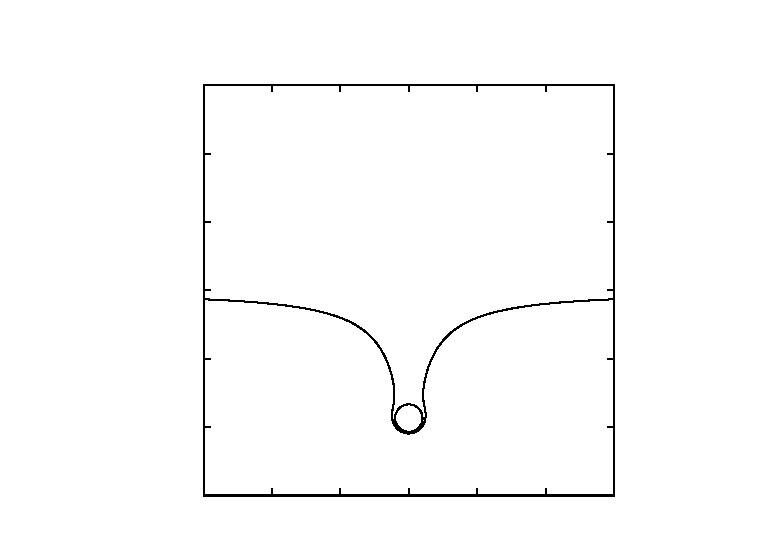
\includegraphics{../../Programming/sinking_bim_write_up/trunk/sphere_frame}}%
    \gplfronttext
  \end{picture}%
\endgroup
}
        \caption{}
        \label{fig:sphere_sink}
      \end{subfigure}
      ~
      \begin{subfigure}[b]{0.45\textwidth}
        \resizebox{\textwidth}{!}{\Large % GNUPLOT: LaTeX picture with Postscript
\begingroup
  \makeatletter
  \providecommand\color[2][]{%
    \GenericError{(gnuplot) \space\space\space\@spaces}{%
      Package color not loaded in conjunction with
      terminal option `colourtext'%
    }{See the gnuplot documentation for explanation.%
    }{Either use 'blacktext' in gnuplot or load the package
      color.sty in LaTeX.}%
    \renewcommand\color[2][]{}%
  }%
  \providecommand\includegraphics[2][]{%
    \GenericError{(gnuplot) \space\space\space\@spaces}{%
      Package graphicx or graphics not loaded%
    }{See the gnuplot documentation for explanation.%
    }{The gnuplot epslatex terminal needs graphicx.sty or graphics.sty.}%
    \renewcommand\includegraphics[2][]{}%
  }%
  \providecommand\rotatebox[2]{#2}%
  \@ifundefined{ifGPcolor}{%
    \newif\ifGPcolor
    \GPcolorfalse
  }{}%
  \@ifundefined{ifGPblacktext}{%
    \newif\ifGPblacktext
    \GPblacktexttrue
  }{}%
  % define a \g@addto@macro without @ in the name:
  \let\gplgaddtomacro\g@addto@macro
  % define empty templates for all commands taking text:
  \gdef\gplbacktext{}%
  \gdef\gplfronttext{}%
  \makeatother
  \ifGPblacktext
    % no textcolor at all
    \def\colorrgb#1{}%
    \def\colorgray#1{}%
  \else
    % gray or color?
    \ifGPcolor
      \def\colorrgb#1{\color[rgb]{#1}}%
      \def\colorgray#1{\color[gray]{#1}}%
      \expandafter\def\csname LTw\endcsname{\color{white}}%
      \expandafter\def\csname LTb\endcsname{\color{black}}%
      \expandafter\def\csname LTa\endcsname{\color{black}}%
      \expandafter\def\csname LT0\endcsname{\color[rgb]{1,0,0}}%
      \expandafter\def\csname LT1\endcsname{\color[rgb]{0,1,0}}%
      \expandafter\def\csname LT2\endcsname{\color[rgb]{0,0,1}}%
      \expandafter\def\csname LT3\endcsname{\color[rgb]{1,0,1}}%
      \expandafter\def\csname LT4\endcsname{\color[rgb]{0,1,1}}%
      \expandafter\def\csname LT5\endcsname{\color[rgb]{1,1,0}}%
      \expandafter\def\csname LT6\endcsname{\color[rgb]{0,0,0}}%
      \expandafter\def\csname LT7\endcsname{\color[rgb]{1,0.3,0}}%
      \expandafter\def\csname LT8\endcsname{\color[rgb]{0.5,0.5,0.5}}%
    \else
      % gray
      \def\colorrgb#1{\color{black}}%
      \def\colorgray#1{\color[gray]{#1}}%
      \expandafter\def\csname LTw\endcsname{\color{white}}%
      \expandafter\def\csname LTb\endcsname{\color{black}}%
      \expandafter\def\csname LTa\endcsname{\color{black}}%
      \expandafter\def\csname LT0\endcsname{\color{black}}%
      \expandafter\def\csname LT1\endcsname{\color{black}}%
      \expandafter\def\csname LT2\endcsname{\color{black}}%
      \expandafter\def\csname LT3\endcsname{\color{black}}%
      \expandafter\def\csname LT4\endcsname{\color{black}}%
      \expandafter\def\csname LT5\endcsname{\color{black}}%
      \expandafter\def\csname LT6\endcsname{\color{black}}%
      \expandafter\def\csname LT7\endcsname{\color{black}}%
      \expandafter\def\csname LT8\endcsname{\color{black}}%
    \fi
  \fi
    \setlength{\unitlength}{0.0500bp}%
    \ifx\gptboxheight\undefined%
      \newlength{\gptboxheight}%
      \newlength{\gptboxwidth}%
      \newsavebox{\gptboxtext}%
    \fi%
    \setlength{\fboxrule}{0.5pt}%
    \setlength{\fboxsep}{1pt}%
\begin{picture}(7200.00,5040.00)%
    \gplgaddtomacro\gplbacktext{%
      \csname LTb\endcsname%
      \put(1663,440){\makebox(0,0)[r]{\strut{}$-15$}}%
      \put(1663,1097){\makebox(0,0)[r]{\strut{}$-10$}}%
      \put(1663,1753){\makebox(0,0)[r]{\strut{}$-5$}}%
      \put(1663,2410){\makebox(0,0)[r]{\strut{}$0$}}%
      \put(1663,3066){\makebox(0,0)[r]{\strut{}$5$}}%
      \put(1663,3723){\makebox(0,0)[r]{\strut{}$10$}}%
      \put(1663,4379){\makebox(0,0)[r]{\strut{}$15$}}%
      \put(1795,220){\makebox(0,0){\strut{}$-15$}}%
      \put(2452,220){\makebox(0,0){\strut{}$-10$}}%
      \put(3108,220){\makebox(0,0){\strut{}$-5$}}%
      \put(3765,220){\makebox(0,0){\strut{}$0$}}%
      \put(4421,220){\makebox(0,0){\strut{}$5$}}%
      \put(5078,220){\makebox(0,0){\strut{}$10$}}%
      \put(5734,220){\makebox(0,0){\strut{}$15$}}%
    }%
    \gplgaddtomacro\gplfronttext{%
      \csname LTb\endcsname%
      \put(3764,4709){\makebox(0,0){\strut{}t = 26.83}}%
    }%
    \gplbacktext
    \put(0,0){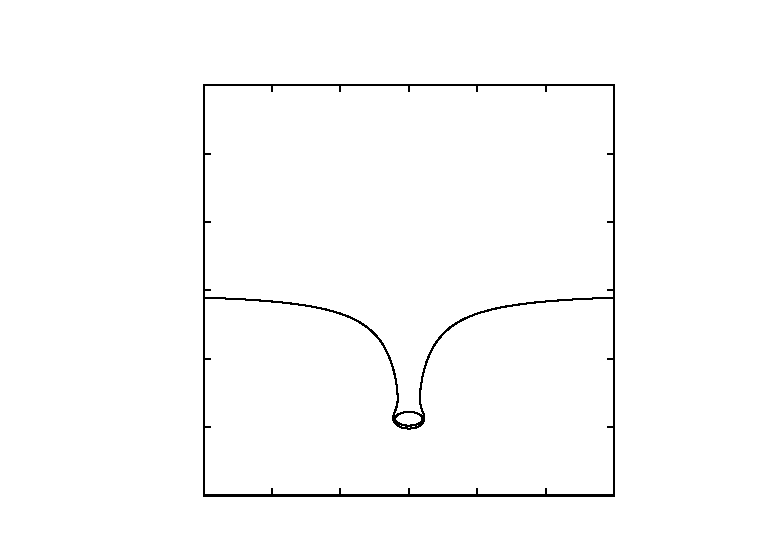
\includegraphics{../../Programming/sinking_bim_write_up/trunk/ob_frame}}%
    \gplfronttext
  \end{picture}%
\endgroup
}
        \caption{}
        \label{fig:ob_sink}
      \end{subfigure}
      \caption{Comparing the sinking of a a) sphere and an b) oblate spheroid with $R = 0.5$ for $D = \Bo = 1000$ and $\lambda = 1$. Both interfacial profiles are very similar.}\label{fig:sinking_comp}
    \end{figure}

\section{Discussion}
\label{sec:discuss}


\subsection{Floating versus Sinking}
\label{subsec:float_sink_discuss}

Figure~\ref{fig:zoom_regime} shows the location of the floating and sinking regimes in the parameter space defined by $\Bo$ and $D$, as found using the BIM presented in sections~\ref{sec:theory} and~\ref{sec:num_meth}. The curve in the figure shows the prediction for the transition between the two regimes found from the model of \citet{Vella06} for a contact angle of $\pi$ (sphere is completely wetted by upper fluid). It can be see that for a given $\Bo$, the transition predicted by the BIM is found at a higher value of $D$ than for the model presented by \citet{Vella06}. To rationalise this discrepancy, a brief description of the \citet{Vella06} model is given here, highlighting the key differences with the BIM. Motivated by these differences, modifications are then proposed to the \citet{Vella06} model and the validity of these is determined by comparing with the results from the BIM.

\subsubsection{\citet{Vella06} Model: A static description of the floating - sinking transition}
\label{subsubsec:Vella_model}

The model proposed in \citet{Vella06} considers the static problem of a sphere sitting at the interface between two immiscible, density stratified fluids. The presence of a three-phase contact line is assumed. The configuration is as seen in figure~\ref{fig:Vella_config}. The model is a force balance of the surface tension, buoyancy and gravitational forces present in the system, and finds the condition for there to be an equilibrium position of the sphere at the interface. 

  \begin{figure}
    $$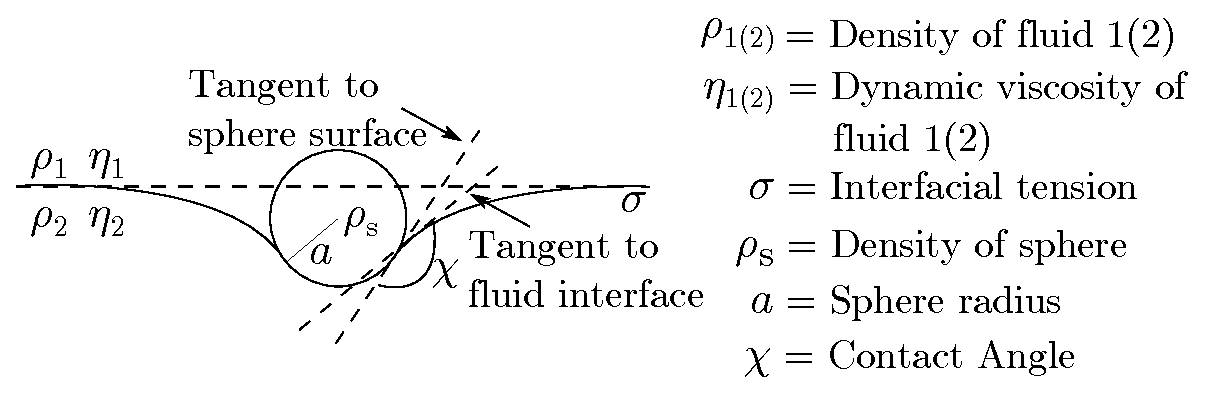
\includegraphics[width=0.8\textwidth]{../../Programming/sinking_bim_write_up/trunk/physical_formulation.eps}$$
    \caption{The configuration of the problem as modelled by \citet{Vella06}. The key difference between this and the BIM presented in sections~\ref{sec:theory} and~\ref{sec:num_meth} is that this model is static, and a three phase contact line is assumed. \label{fig:Vella_config}}
  \end{figure}

In order to construct this model, it is neccessary to consider a result from \citet{Keller98}; the vertical contribution of the IFT force on an object floating at an interface is equivalent to the buoyancy force of the fluid in the meniscus. This was first hypothesised by Galilei \citep{Galilei1663, Vella(2)07}. Figure~\ref{fig:Keller_fig} is a useful aid in explaining this. The volume of the meniscus is shown by the shaded regions external to the vertical cylindrical surface which contains the contact line. The IFT contribution to the vertical force is equal to the buoyancy of the upper fluid in this region. This means the force baclance for a sphere in equilibrium can be expressed as

\begin{equation}
\label{equ:Vella_force}
\frac{4 \pi (\rho_{\text{s}} - \rho_{1}) a^{3} g}{3} = 2 \pi a \sigma \sin \theta_{\text{c}} \sin (\chi - \theta_{\text{c}}) + (\rho_{2} - \rho_{1}) g \left(\frac{\pi a^{3} (2 + 3 \cos \theta_{\text{c}} - \cos^{3} \theta_{\text{c}})}{3} - \pi z_{c} a^{2} \sin^{2} \theta_{\text{c}} \right)
\end{equation}

where $\theta_{\text{c}}$ and $z_{\text{c}}$ are the polar and vertical coordinates of the contact line respectively. The left hand side corresponds to the weight of the sphere relative to the weight of the same volume of the upper fluid. The right hand side is the sum of the IFT contribution (equivalent to the buoyant force due to the volume of the meniscus external to the contact line), and the displaced weight of the lower fluid relative to the upper fluid, in the volume of the meniscus internal to the contact line (central shaded region in figure~\ref{fig:Keller_fig}).

\begin{figure}
  $$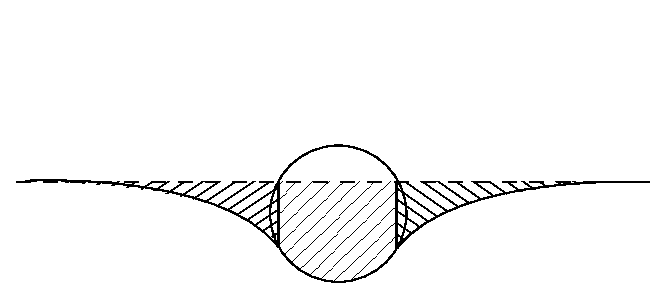
\includegraphics[width=0.8\textwidth]{../../Programming/sinking_bim_write_up/trunk/Keller_fig.eps}$$
  \caption{The different shadings show the regions internal and external to the meniscus.  \label{fig:Keller_fig}}
\end{figure}

Using the non-dimensionalisation scheme presented in section~\ref{subsec:theory} the force balance can be written as

\begin{equation}
\label{equ:Vella_non_dim}
D = \frac{3 \sin \theta_{\text{c}} \sin(\chi - \theta_{\text{c}})}{2 \Bo} + \frac{2 + 3 \cos \theta_{\text{c}} - \cos^{3} \theta_{\text{c}}}{3} - \frac{3 z'_{\text{c}} \sin^{2}\theta_{\text{c}}}{4}
\end{equation}

For a given $\Bo$, contact angle $\chi$ and contact line position (given by $\theta_{\text{c}}$ and $z'_{\text{c}}$), this equation gives the largest possible value of $D$ for which an equilibrium floating position exists. The contact line position itself is found by solving the Laplace-Young equation for the interfacial profile subject to the boundary condition given by the contact angle condition on the sphere, and imposing that the interface returns to its equilibrium position away from the sphere. This is a boundary value problem \citep{Riley06} and has no analytical solution in an axisymmetric geometry so needs to be solved numerically. 

Hence, the routine for finding the maximum $D$ at which floating can occur for a given $\Bo$ and $\chi$ is found by sweeping over different values of $\theta_{\text{c}}$ between $0$ and $\pi$ and solving the Laplace-Young equation for the corresponding height of the contact line $z_{\text{c}}$ for each case. These are then substituted into equation~\ref{equ:Vella_non_dim}. The largest value of $D$ calculated in the sweep is the largest value of $D$ for which floating is possible for a given $\Bo$ and $\chi$. The curve shown in figure~\ref{fig:zoom_regime} is the predicted floating-sinking transition for $\chi = pi$.

\subsubsection{Difference between the static and BIM models}
\label{subsubsec:model_diff}

To explain the discrepancy between the two models in their prediction of the floating-sinking transition location in the $\Bo$-$D$ parameters space, it is important to consider the differences between the models. The static model, as suggested by its name, is static. It merely considers the conditions at which a sphere can be in equilibrium at an interface, given a contact line exists. It doesn't account for any prior motion of the sphere. It has been shown for cylinders and a liquid-gas interface that increasing the speed of impact reduces the maximum density and/or size of cylinder that can float at the interface \citet{Vella07, Vella10}. This situation is theoretically considered by using an initial condition of the cylinder being in contact with the interface but having some initial velocity. It is important to note that in these studies the flow is in the inertial regime.

The key difference with the BIM used in this study is that in the initial state of the system the sphere is multiple radii above the interface and is settling at its terminal velocity. Hence, as well as having an initial velocity, no contact line exists. Since there is a no-slip boundary condition on the surface of the sphere (equation~\ref{equ:BC_kin_spere}), the fluid immediately adjacent to the sphere will never be displaced. This means that there will always remain a layer of upper phase fluid between the sphere and the interface. Hence it is impossible to reproduce the film drainage mode as seen in the experimental study. The presence of this layer will also have an effect on the floating-sinking transition, since it is effectively provides an extra contribution to the upward buoyancy forces. 

For a given $\Bo$, the BIM predicts the value of $D$ at which the floating-sinking transition occurs to be positively displaced relative to the prediction from the static model. This suggests that the effect of the trapped layer of upper phase fluid between the sphere and the interface has a more significant effect than the impact of the sphere.

\subsubsection{Modified static model}
\label{subsubsec:mod_stat_mod}

Motivated by the observation that the trapped layer has a greater effect on the floating-sinking transition than the impact of the sphere, a static model, modified from that described in section~\ref{subsubsec:Vella_model}, is presented here which accounts for a trapped layer of upper phase fluid (figure~\ref{fig:mod_stat_mod}). For simplicity, this layer is assumed to have a uniform thickness. Hence, in this model, the interface can be described by two parts. The first is a spherical cap of radius $a + \delta$ concentric with the sphere. At some polar angle $\theta_{\text{c}}$ this transitions into a meniscus whose geometry is determined by the Laplace-Young equation subject to the condition that at $\theta = \theta_{\text{c}}$, the tangent planes to both the spherical cap and the meniscus are coincident. 

\begin{figure}
  $$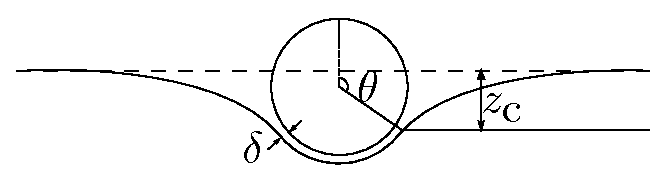
\includegraphics[width=0.8\textwidth]{../../Programming/sinking_bim_write_up/trunk/mod_stat_mod.eps}$$
  \caption{The modified static model configuration. The sphere and the interface are separated by a film of upper phase fluid of constant thickness $\delta$. \label{fig:mod_stat_mod}}
\end{figure}

The force balance for this geometry can be realised by modifying equation~\ref{equ:Vella_force} by replacing all the occurences of $a$ on the right-hand side by $a + \delta$ and setting $\chi = \pi$;

\begin{equation}
\label{equ:mod_force}
\frac{4 \pi (\rho_{\text{s}} - \rho_{1}) a^{3} g}{3} = 2 \pi (a + \delta) \sigma \sin^{2} \theta_{\text{c}} + (\rho_{2} - \rho_{1}) g \left(\frac{\pi (a + \delta)^{3} (2 + 3 \cos \theta_{\text{c}} - \cos^{3} \theta_{\text{c}})}{3} - \pi z_{c} (a + \delta)^{2} \sin^{2} \theta_{\text{c}} \right).
\end{equation}

As in section~\ref{subsubsec:Vella_model}, this can be non dimensionalised to give

\begin{equation}
\label{equ:mod_non_dim}
D = \Delta^{1/2} \left(\frac{3 \sin^{2} \theta_{\text{c}}}{2 \Bo} + \frac{\Delta (2 + 3 \cos \theta_{\text{c}} - \cos^{3} \theta_{\text{c}})}{4} - \frac{3 z'_{\text{c}} \Delta^{1/2} \sin^{2} \theta_{\text{c}}}{4}\right)
\end{equation}

where

\begin{equation}
\label{equ:non_dim_film}
\Delta = \left(1 + \frac{\delta}{a}\right)^{2}.
\end{equation}

For a given $\Bo$, $\theta_{\text{c}}$ and $\Delta$, equation~\ref{equ:mod_non_dim} gives the maximum value of $D$ for which a sphere is in equilibrium whilst separated from an interface by a film of thickness $\delta$. Using a routine similar to that described in section~\ref{subsubsec:Vella_model} the floating-sinking transition in the $\Bo$-$D$ space for different $\delta$ can be found (figure~\ref{fig:Delta_trans}). It can be seen that increasing the value of $\Delta$. and so the relative thickness of the trapped film, it is possible to support denser and larger spheres at a fluid interface. This is intuitively explained by the additional contribution of the buoyant fluid in the film to the upward force.

  \begin{figure}
    \resizebox{0.9\textwidth}{!}{\large % GNUPLOT: LaTeX picture with Postscript
\begingroup
  \makeatletter
  \providecommand\color[2][]{%
    \GenericError{(gnuplot) \space\space\space\@spaces}{%
      Package color not loaded in conjunction with
      terminal option `colourtext'%
    }{See the gnuplot documentation for explanation.%
    }{Either use 'blacktext' in gnuplot or load the package
      color.sty in LaTeX.}%
    \renewcommand\color[2][]{}%
  }%
  \providecommand\includegraphics[2][]{%
    \GenericError{(gnuplot) \space\space\space\@spaces}{%
      Package graphicx or graphics not loaded%
    }{See the gnuplot documentation for explanation.%
    }{The gnuplot epslatex terminal needs graphicx.sty or graphics.sty.}%
    \renewcommand\includegraphics[2][]{}%
  }%
  \providecommand\rotatebox[2]{#2}%
  \@ifundefined{ifGPcolor}{%
    \newif\ifGPcolor
    \GPcolorfalse
  }{}%
  \@ifundefined{ifGPblacktext}{%
    \newif\ifGPblacktext
    \GPblacktexttrue
  }{}%
  % define a \g@addto@macro without @ in the name:
  \let\gplgaddtomacro\g@addto@macro
  % define empty templates for all commands taking text:
  \gdef\gplbacktext{}%
  \gdef\gplfronttext{}%
  \makeatother
  \ifGPblacktext
    % no textcolor at all
    \def\colorrgb#1{}%
    \def\colorgray#1{}%
  \else
    % gray or color?
    \ifGPcolor
      \def\colorrgb#1{\color[rgb]{#1}}%
      \def\colorgray#1{\color[gray]{#1}}%
      \expandafter\def\csname LTw\endcsname{\color{white}}%
      \expandafter\def\csname LTb\endcsname{\color{black}}%
      \expandafter\def\csname LTa\endcsname{\color{black}}%
      \expandafter\def\csname LT0\endcsname{\color[rgb]{1,0,0}}%
      \expandafter\def\csname LT1\endcsname{\color[rgb]{0,1,0}}%
      \expandafter\def\csname LT2\endcsname{\color[rgb]{0,0,1}}%
      \expandafter\def\csname LT3\endcsname{\color[rgb]{1,0,1}}%
      \expandafter\def\csname LT4\endcsname{\color[rgb]{0,1,1}}%
      \expandafter\def\csname LT5\endcsname{\color[rgb]{1,1,0}}%
      \expandafter\def\csname LT6\endcsname{\color[rgb]{0,0,0}}%
      \expandafter\def\csname LT7\endcsname{\color[rgb]{1,0.3,0}}%
      \expandafter\def\csname LT8\endcsname{\color[rgb]{0.5,0.5,0.5}}%
    \else
      % gray
      \def\colorrgb#1{\color{black}}%
      \def\colorgray#1{\color[gray]{#1}}%
      \expandafter\def\csname LTw\endcsname{\color{white}}%
      \expandafter\def\csname LTb\endcsname{\color{black}}%
      \expandafter\def\csname LTa\endcsname{\color{black}}%
      \expandafter\def\csname LT0\endcsname{\color{black}}%
      \expandafter\def\csname LT1\endcsname{\color{black}}%
      \expandafter\def\csname LT2\endcsname{\color{black}}%
      \expandafter\def\csname LT3\endcsname{\color{black}}%
      \expandafter\def\csname LT4\endcsname{\color{black}}%
      \expandafter\def\csname LT5\endcsname{\color{black}}%
      \expandafter\def\csname LT6\endcsname{\color{black}}%
      \expandafter\def\csname LT7\endcsname{\color{black}}%
      \expandafter\def\csname LT8\endcsname{\color{black}}%
    \fi
  \fi
    \setlength{\unitlength}{0.0500bp}%
    \ifx\gptboxheight\undefined%
      \newlength{\gptboxheight}%
      \newlength{\gptboxwidth}%
      \newsavebox{\gptboxtext}%
    \fi%
    \setlength{\fboxrule}{0.5pt}%
    \setlength{\fboxsep}{1pt}%
\begin{picture}(7200.00,5040.00)%
    \gplgaddtomacro\gplbacktext{%
      \csname LTb\endcsname%
      \put(682,704){\makebox(0,0)[r]{\strut{}$0$}}%
      \put(682,1213){\makebox(0,0)[r]{\strut{}$2$}}%
      \put(682,1722){\makebox(0,0)[r]{\strut{}$4$}}%
      \put(682,2231){\makebox(0,0)[r]{\strut{}$6$}}%
      \put(682,2740){\makebox(0,0)[r]{\strut{}$8$}}%
      \put(682,3248){\makebox(0,0)[r]{\strut{}$10$}}%
      \put(682,3757){\makebox(0,0)[r]{\strut{}$12$}}%
      \put(682,4266){\makebox(0,0)[r]{\strut{}$14$}}%
      \put(682,4775){\makebox(0,0)[r]{\strut{}$16$}}%
      \put(814,484){\makebox(0,0){\strut{}$0$}}%
      \put(2012,484){\makebox(0,0){\strut{}$2$}}%
      \put(3210,484){\makebox(0,0){\strut{}$4$}}%
      \put(4407,484){\makebox(0,0){\strut{}$6$}}%
      \put(5605,484){\makebox(0,0){\strut{}$8$}}%
      \put(6803,484){\makebox(0,0){\strut{}$10$}}%
    }%
    \gplgaddtomacro\gplfronttext{%
      \csname LTb\endcsname%
      \put(176,2739){\rotatebox{-270}{\makebox(0,0){\strut{}$D$}}}%
      \put(3808,154){\makebox(0,0){\strut{}$\Bo$}}%
      \put(5979,4602){\makebox(0,0){\strut{}$\Delta$}}%
      \csname LTb\endcsname%
      \put(5816,4382){\makebox(0,0)[r]{\strut{}$1$}}%
      \csname LTb\endcsname%
      \put(5816,4162){\makebox(0,0)[r]{\strut{}$1.21$}}%
      \csname LTb\endcsname%
      \put(5816,3942){\makebox(0,0)[r]{\strut{}$1.44$}}%
      \csname LTb\endcsname%
      \put(5816,3722){\makebox(0,0)[r]{\strut{}$1.69$}}%
      \csname LTb\endcsname%
      \put(5816,3502){\makebox(0,0)[r]{\strut{}$1.96$}}%
      \csname LTb\endcsname%
      \put(5816,3282){\makebox(0,0)[r]{\strut{}$2.25$}}%
    }%
    \gplbacktext
    \put(0,0){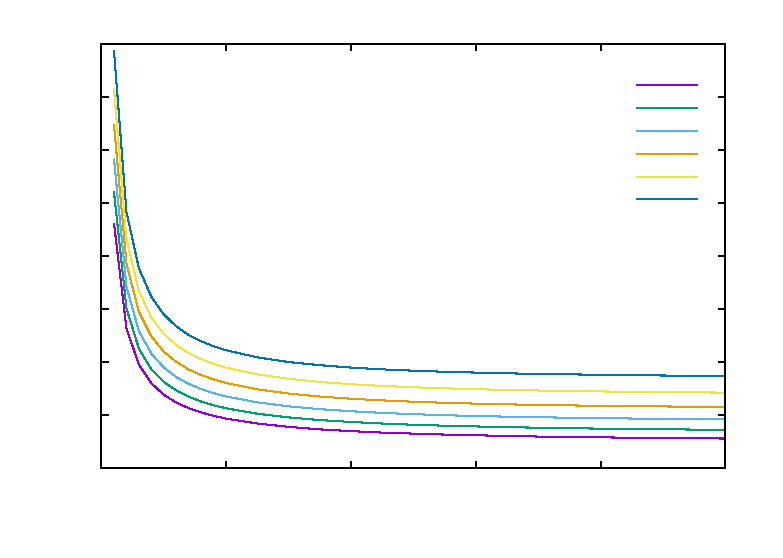
\includegraphics{Delta_trans_pub}}%
    \gplfronttext
  \end{picture}%
\endgroup
}
    \caption{Plots of equation~\ref{equ:mod_non_dim} for different values of $\Delta$. As $\Delta$ increases the floating-sinking transition at a given value of $\Bo$ shifts to higher values of $D$. \label{fig:Delta_trans}}
  \end{figure}

\subsubsection{Comparison with BIM results}
\label{subsubsection:mod_comp_bim}

To test if the modified static model provides a suitable explanation for the observed floating-sinking transition in the BIM results, the results of four simulations where floating was observed but the parameters are close to the transition were chosen for further analysis (see table~\ref{tab:film_sims}). For each of these simulations, the final profile of the thickness of the film separating the sphere from the interface was considered (figure~\ref{fig:float_films}) and the mean thickness of the film, weighted by the radial coordinate of the fluid, was calculated (given in table~\ref{tab:film_sims}).

\begin{longtable}{|c|c|c|c|}
  \caption{BIM simulations chosen for comparison with the modified static model, and the mean final thickness of the film separating the sphere from the interface. \label{tab:film_sims}} \\ % title name of the table
  \hline
$D$ & $\Bo$ & $\bar{\delta}$ & $\Delta$ \\
  \hline % inserts single-line
  3.4 & 1.0 & 0.175 & 1.381 \\
  2.8 & 1.5 & 0.171 & 1.371 \\
  2.2 & 2.5 & 0.160 & 1.346 \\
  2.0 & 3.5 & 0.157 & 1.339 \\
  \hline
\end{longtable}

    \begin{figure}
      \centering
      \begin{subfigure}[b]{0.225\textwidth}
        \resizebox{\textwidth}{!}{\Huge % GNUPLOT: LaTeX picture with Postscript
\begingroup
  \makeatletter
  \providecommand\color[2][]{%
    \GenericError{(gnuplot) \space\space\space\@spaces}{%
      Package color not loaded in conjunction with
      terminal option `colourtext'%
    }{See the gnuplot documentation for explanation.%
    }{Either use 'blacktext' in gnuplot or load the package
      color.sty in LaTeX.}%
    \renewcommand\color[2][]{}%
  }%
  \providecommand\includegraphics[2][]{%
    \GenericError{(gnuplot) \space\space\space\@spaces}{%
      Package graphicx or graphics not loaded%
    }{See the gnuplot documentation for explanation.%
    }{The gnuplot epslatex terminal needs graphicx.sty or graphics.sty.}%
    \renewcommand\includegraphics[2][]{}%
  }%
  \providecommand\rotatebox[2]{#2}%
  \@ifundefined{ifGPcolor}{%
    \newif\ifGPcolor
    \GPcolorfalse
  }{}%
  \@ifundefined{ifGPblacktext}{%
    \newif\ifGPblacktext
    \GPblacktexttrue
  }{}%
  % define a \g@addto@macro without @ in the name:
  \let\gplgaddtomacro\g@addto@macro
  % define empty templates for all commands taking text:
  \gdef\gplbacktext{}%
  \gdef\gplfronttext{}%
  \makeatother
  \ifGPblacktext
    % no textcolor at all
    \def\colorrgb#1{}%
    \def\colorgray#1{}%
  \else
    % gray or color?
    \ifGPcolor
      \def\colorrgb#1{\color[rgb]{#1}}%
      \def\colorgray#1{\color[gray]{#1}}%
      \expandafter\def\csname LTw\endcsname{\color{white}}%
      \expandafter\def\csname LTb\endcsname{\color{black}}%
      \expandafter\def\csname LTa\endcsname{\color{black}}%
      \expandafter\def\csname LT0\endcsname{\color[rgb]{1,0,0}}%
      \expandafter\def\csname LT1\endcsname{\color[rgb]{0,1,0}}%
      \expandafter\def\csname LT2\endcsname{\color[rgb]{0,0,1}}%
      \expandafter\def\csname LT3\endcsname{\color[rgb]{1,0,1}}%
      \expandafter\def\csname LT4\endcsname{\color[rgb]{0,1,1}}%
      \expandafter\def\csname LT5\endcsname{\color[rgb]{1,1,0}}%
      \expandafter\def\csname LT6\endcsname{\color[rgb]{0,0,0}}%
      \expandafter\def\csname LT7\endcsname{\color[rgb]{1,0.3,0}}%
      \expandafter\def\csname LT8\endcsname{\color[rgb]{0.5,0.5,0.5}}%
    \else
      % gray
      \def\colorrgb#1{\color{black}}%
      \def\colorgray#1{\color[gray]{#1}}%
      \expandafter\def\csname LTw\endcsname{\color{white}}%
      \expandafter\def\csname LTb\endcsname{\color{black}}%
      \expandafter\def\csname LTa\endcsname{\color{black}}%
      \expandafter\def\csname LT0\endcsname{\color{black}}%
      \expandafter\def\csname LT1\endcsname{\color{black}}%
      \expandafter\def\csname LT2\endcsname{\color{black}}%
      \expandafter\def\csname LT3\endcsname{\color{black}}%
      \expandafter\def\csname LT4\endcsname{\color{black}}%
      \expandafter\def\csname LT5\endcsname{\color{black}}%
      \expandafter\def\csname LT6\endcsname{\color{black}}%
      \expandafter\def\csname LT7\endcsname{\color{black}}%
      \expandafter\def\csname LT8\endcsname{\color{black}}%
    \fi
  \fi
    \setlength{\unitlength}{0.0500bp}%
    \ifx\gptboxheight\undefined%
      \newlength{\gptboxheight}%
      \newlength{\gptboxwidth}%
      \newsavebox{\gptboxtext}%
    \fi%
    \setlength{\fboxrule}{0.5pt}%
    \setlength{\fboxsep}{1pt}%
\begin{picture}(5668.00,8502.00)%
    \gplgaddtomacro\gplbacktext{%
      \csname LTb\endcsname%
      \put(946,1128){\makebox(0,0)[r]{\strut{}$-2.5$}}%
      \put(946,2176){\makebox(0,0)[r]{\strut{}$-2$}}%
      \put(946,3224){\makebox(0,0)[r]{\strut{}$-1.5$}}%
      \put(946,4273){\makebox(0,0)[r]{\strut{}$-1$}}%
      \put(946,5321){\makebox(0,0)[r]{\strut{}$-0.5$}}%
      \put(946,6369){\makebox(0,0)[r]{\strut{}$0$}}%
      \put(946,7417){\makebox(0,0)[r]{\strut{}$0.5$}}%
      \put(1078,908){\makebox(0,0){\strut{}$0$}}%
      \put(2126,908){\makebox(0,0){\strut{}$0.5$}}%
      \put(3175,908){\makebox(0,0){\strut{}$1$}}%
      \put(4223,908){\makebox(0,0){\strut{}$1.5$}}%
      \put(5271,908){\makebox(0,0){\strut{}$2$}}%
    }%
    \gplgaddtomacro\gplfronttext{%
      \csname LTb\endcsname%
      \put(176,4272){\rotatebox{-270}{\makebox(0,0){\strut{}$z$}}}%
      \put(3174,578){\makebox(0,0){\strut{}$r$}}%
      \put(3174,7747){\makebox(0,0){\strut{}$\Bo = 1$, $D = 3.4$}}%
    }%
    \gplbacktext
    \put(0,0){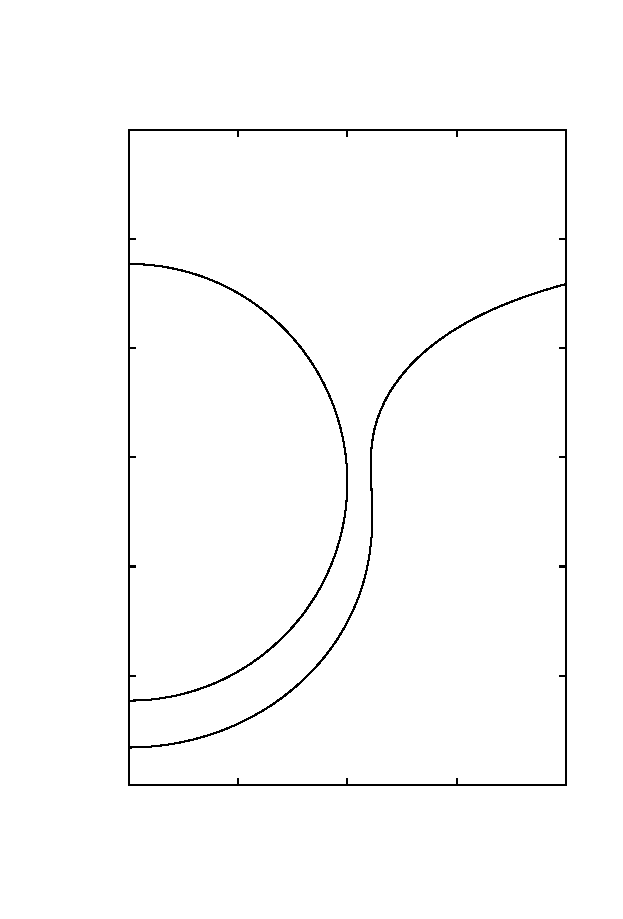
\includegraphics{float1}}%
    \gplfronttext
  \end{picture}%
\endgroup
}
        \caption{}
        \label{fig:float1}
      \end{subfigure}
      ~
      \begin{subfigure}[b]{0.225\textwidth}
        \resizebox{\textwidth}{!}{\Huge % GNUPLOT: LaTeX picture with Postscript
\begingroup
  \makeatletter
  \providecommand\color[2][]{%
    \GenericError{(gnuplot) \space\space\space\@spaces}{%
      Package color not loaded in conjunction with
      terminal option `colourtext'%
    }{See the gnuplot documentation for explanation.%
    }{Either use 'blacktext' in gnuplot or load the package
      color.sty in LaTeX.}%
    \renewcommand\color[2][]{}%
  }%
  \providecommand\includegraphics[2][]{%
    \GenericError{(gnuplot) \space\space\space\@spaces}{%
      Package graphicx or graphics not loaded%
    }{See the gnuplot documentation for explanation.%
    }{The gnuplot epslatex terminal needs graphicx.sty or graphics.sty.}%
    \renewcommand\includegraphics[2][]{}%
  }%
  \providecommand\rotatebox[2]{#2}%
  \@ifundefined{ifGPcolor}{%
    \newif\ifGPcolor
    \GPcolorfalse
  }{}%
  \@ifundefined{ifGPblacktext}{%
    \newif\ifGPblacktext
    \GPblacktexttrue
  }{}%
  % define a \g@addto@macro without @ in the name:
  \let\gplgaddtomacro\g@addto@macro
  % define empty templates for all commands taking text:
  \gdef\gplbacktext{}%
  \gdef\gplfronttext{}%
  \makeatother
  \ifGPblacktext
    % no textcolor at all
    \def\colorrgb#1{}%
    \def\colorgray#1{}%
  \else
    % gray or color?
    \ifGPcolor
      \def\colorrgb#1{\color[rgb]{#1}}%
      \def\colorgray#1{\color[gray]{#1}}%
      \expandafter\def\csname LTw\endcsname{\color{white}}%
      \expandafter\def\csname LTb\endcsname{\color{black}}%
      \expandafter\def\csname LTa\endcsname{\color{black}}%
      \expandafter\def\csname LT0\endcsname{\color[rgb]{1,0,0}}%
      \expandafter\def\csname LT1\endcsname{\color[rgb]{0,1,0}}%
      \expandafter\def\csname LT2\endcsname{\color[rgb]{0,0,1}}%
      \expandafter\def\csname LT3\endcsname{\color[rgb]{1,0,1}}%
      \expandafter\def\csname LT4\endcsname{\color[rgb]{0,1,1}}%
      \expandafter\def\csname LT5\endcsname{\color[rgb]{1,1,0}}%
      \expandafter\def\csname LT6\endcsname{\color[rgb]{0,0,0}}%
      \expandafter\def\csname LT7\endcsname{\color[rgb]{1,0.3,0}}%
      \expandafter\def\csname LT8\endcsname{\color[rgb]{0.5,0.5,0.5}}%
    \else
      % gray
      \def\colorrgb#1{\color{black}}%
      \def\colorgray#1{\color[gray]{#1}}%
      \expandafter\def\csname LTw\endcsname{\color{white}}%
      \expandafter\def\csname LTb\endcsname{\color{black}}%
      \expandafter\def\csname LTa\endcsname{\color{black}}%
      \expandafter\def\csname LT0\endcsname{\color{black}}%
      \expandafter\def\csname LT1\endcsname{\color{black}}%
      \expandafter\def\csname LT2\endcsname{\color{black}}%
      \expandafter\def\csname LT3\endcsname{\color{black}}%
      \expandafter\def\csname LT4\endcsname{\color{black}}%
      \expandafter\def\csname LT5\endcsname{\color{black}}%
      \expandafter\def\csname LT6\endcsname{\color{black}}%
      \expandafter\def\csname LT7\endcsname{\color{black}}%
      \expandafter\def\csname LT8\endcsname{\color{black}}%
    \fi
  \fi
    \setlength{\unitlength}{0.0500bp}%
    \ifx\gptboxheight\undefined%
      \newlength{\gptboxheight}%
      \newlength{\gptboxwidth}%
      \newsavebox{\gptboxtext}%
    \fi%
    \setlength{\fboxrule}{0.5pt}%
    \setlength{\fboxsep}{1pt}%
\begin{picture}(5668.00,8502.00)%
    \gplgaddtomacro\gplbacktext{%
      \csname LTb\endcsname%
      \put(946,1128){\makebox(0,0)[r]{\strut{}$-2.5$}}%
      \put(946,2176){\makebox(0,0)[r]{\strut{}$-2$}}%
      \put(946,3224){\makebox(0,0)[r]{\strut{}$-1.5$}}%
      \put(946,4273){\makebox(0,0)[r]{\strut{}$-1$}}%
      \put(946,5321){\makebox(0,0)[r]{\strut{}$-0.5$}}%
      \put(946,6369){\makebox(0,0)[r]{\strut{}$0$}}%
      \put(946,7417){\makebox(0,0)[r]{\strut{}$0.5$}}%
      \put(1078,908){\makebox(0,0){\strut{}$0$}}%
      \put(2126,908){\makebox(0,0){\strut{}$0.5$}}%
      \put(3175,908){\makebox(0,0){\strut{}$1$}}%
      \put(4223,908){\makebox(0,0){\strut{}$1.5$}}%
      \put(5271,908){\makebox(0,0){\strut{}$2$}}%
    }%
    \gplgaddtomacro\gplfronttext{%
      \csname LTb\endcsname%
      \put(176,4272){\rotatebox{-270}{\makebox(0,0){\strut{}$z$}}}%
      \put(3174,578){\makebox(0,0){\strut{}$r$}}%
      \put(3174,7747){\makebox(0,0){\strut{}$\Bo = 1.5$, $D = 2.8$}}%
    }%
    \gplbacktext
    \put(0,0){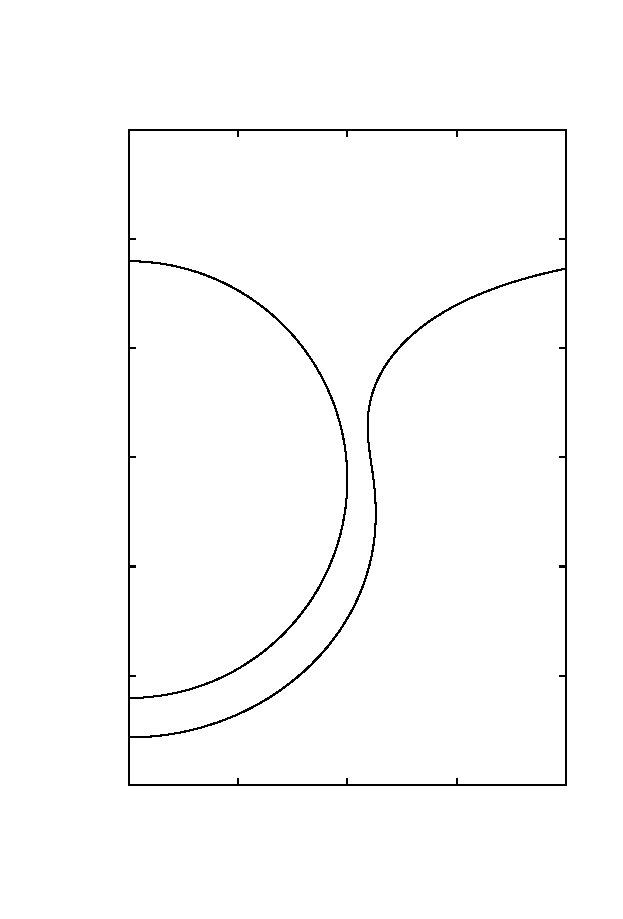
\includegraphics{../../Programming/sinking_bim_write_up/trunk/float2}}%
    \gplfronttext
  \end{picture}%
\endgroup
}
        \caption{}
        \label{fig:float2}
      \end{subfigure}
      ~
      \begin{subfigure}[b]{0.225\textwidth}
        \resizebox{\textwidth}{!}{\Huge % GNUPLOT: LaTeX picture with Postscript
\begingroup
  \makeatletter
  \providecommand\color[2][]{%
    \GenericError{(gnuplot) \space\space\space\@spaces}{%
      Package color not loaded in conjunction with
      terminal option `colourtext'%
    }{See the gnuplot documentation for explanation.%
    }{Either use 'blacktext' in gnuplot or load the package
      color.sty in LaTeX.}%
    \renewcommand\color[2][]{}%
  }%
  \providecommand\includegraphics[2][]{%
    \GenericError{(gnuplot) \space\space\space\@spaces}{%
      Package graphicx or graphics not loaded%
    }{See the gnuplot documentation for explanation.%
    }{The gnuplot epslatex terminal needs graphicx.sty or graphics.sty.}%
    \renewcommand\includegraphics[2][]{}%
  }%
  \providecommand\rotatebox[2]{#2}%
  \@ifundefined{ifGPcolor}{%
    \newif\ifGPcolor
    \GPcolorfalse
  }{}%
  \@ifundefined{ifGPblacktext}{%
    \newif\ifGPblacktext
    \GPblacktexttrue
  }{}%
  % define a \g@addto@macro without @ in the name:
  \let\gplgaddtomacro\g@addto@macro
  % define empty templates for all commands taking text:
  \gdef\gplbacktext{}%
  \gdef\gplfronttext{}%
  \makeatother
  \ifGPblacktext
    % no textcolor at all
    \def\colorrgb#1{}%
    \def\colorgray#1{}%
  \else
    % gray or color?
    \ifGPcolor
      \def\colorrgb#1{\color[rgb]{#1}}%
      \def\colorgray#1{\color[gray]{#1}}%
      \expandafter\def\csname LTw\endcsname{\color{white}}%
      \expandafter\def\csname LTb\endcsname{\color{black}}%
      \expandafter\def\csname LTa\endcsname{\color{black}}%
      \expandafter\def\csname LT0\endcsname{\color[rgb]{1,0,0}}%
      \expandafter\def\csname LT1\endcsname{\color[rgb]{0,1,0}}%
      \expandafter\def\csname LT2\endcsname{\color[rgb]{0,0,1}}%
      \expandafter\def\csname LT3\endcsname{\color[rgb]{1,0,1}}%
      \expandafter\def\csname LT4\endcsname{\color[rgb]{0,1,1}}%
      \expandafter\def\csname LT5\endcsname{\color[rgb]{1,1,0}}%
      \expandafter\def\csname LT6\endcsname{\color[rgb]{0,0,0}}%
      \expandafter\def\csname LT7\endcsname{\color[rgb]{1,0.3,0}}%
      \expandafter\def\csname LT8\endcsname{\color[rgb]{0.5,0.5,0.5}}%
    \else
      % gray
      \def\colorrgb#1{\color{black}}%
      \def\colorgray#1{\color[gray]{#1}}%
      \expandafter\def\csname LTw\endcsname{\color{white}}%
      \expandafter\def\csname LTb\endcsname{\color{black}}%
      \expandafter\def\csname LTa\endcsname{\color{black}}%
      \expandafter\def\csname LT0\endcsname{\color{black}}%
      \expandafter\def\csname LT1\endcsname{\color{black}}%
      \expandafter\def\csname LT2\endcsname{\color{black}}%
      \expandafter\def\csname LT3\endcsname{\color{black}}%
      \expandafter\def\csname LT4\endcsname{\color{black}}%
      \expandafter\def\csname LT5\endcsname{\color{black}}%
      \expandafter\def\csname LT6\endcsname{\color{black}}%
      \expandafter\def\csname LT7\endcsname{\color{black}}%
      \expandafter\def\csname LT8\endcsname{\color{black}}%
    \fi
  \fi
    \setlength{\unitlength}{0.0500bp}%
    \ifx\gptboxheight\undefined%
      \newlength{\gptboxheight}%
      \newlength{\gptboxwidth}%
      \newsavebox{\gptboxtext}%
    \fi%
    \setlength{\fboxrule}{0.5pt}%
    \setlength{\fboxsep}{1pt}%
\begin{picture}(5668.00,8502.00)%
    \gplgaddtomacro\gplbacktext{%
      \csname LTb\endcsname%
      \put(946,1128){\makebox(0,0)[r]{\strut{}$-2.5$}}%
      \put(946,2176){\makebox(0,0)[r]{\strut{}$-2$}}%
      \put(946,3224){\makebox(0,0)[r]{\strut{}$-1.5$}}%
      \put(946,4273){\makebox(0,0)[r]{\strut{}$-1$}}%
      \put(946,5321){\makebox(0,0)[r]{\strut{}$-0.5$}}%
      \put(946,6369){\makebox(0,0)[r]{\strut{}$0$}}%
      \put(946,7417){\makebox(0,0)[r]{\strut{}$0.5$}}%
      \put(1078,908){\makebox(0,0){\strut{}$0$}}%
      \put(2126,908){\makebox(0,0){\strut{}$0.5$}}%
      \put(3175,908){\makebox(0,0){\strut{}$1$}}%
      \put(4223,908){\makebox(0,0){\strut{}$1.5$}}%
      \put(5271,908){\makebox(0,0){\strut{}$2$}}%
    }%
    \gplgaddtomacro\gplfronttext{%
      \csname LTb\endcsname%
      \put(176,4272){\rotatebox{-270}{\makebox(0,0){\strut{}$z$}}}%
      \put(3174,578){\makebox(0,0){\strut{}$r$}}%
      \put(3174,7747){\makebox(0,0){\strut{}$\Bo = 2.5$, $D = 2.2$}}%
    }%
    \gplbacktext
    \put(0,0){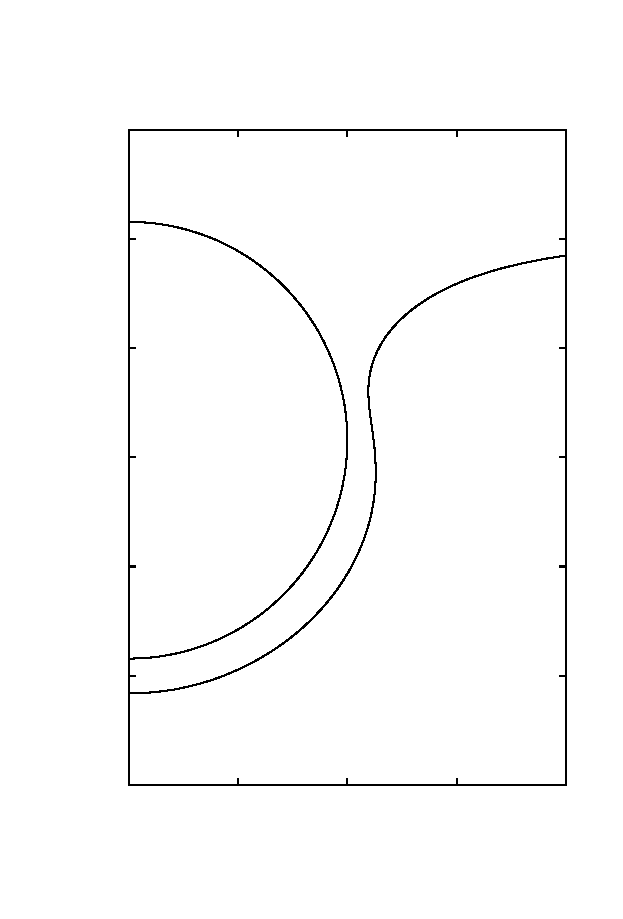
\includegraphics{../../Programming/sinking_bim_write_up/trunk/float3}}%
    \gplfronttext
  \end{picture}%
\endgroup
}
        \caption{}
        \label{fig:float3}
      \end{subfigure}
      ~
      \begin{subfigure}[b]{0.225\textwidth}
        \resizebox{\textwidth}{!}{\Huge % GNUPLOT: LaTeX picture with Postscript
\begingroup
  \makeatletter
  \providecommand\color[2][]{%
    \GenericError{(gnuplot) \space\space\space\@spaces}{%
      Package color not loaded in conjunction with
      terminal option `colourtext'%
    }{See the gnuplot documentation for explanation.%
    }{Either use 'blacktext' in gnuplot or load the package
      color.sty in LaTeX.}%
    \renewcommand\color[2][]{}%
  }%
  \providecommand\includegraphics[2][]{%
    \GenericError{(gnuplot) \space\space\space\@spaces}{%
      Package graphicx or graphics not loaded%
    }{See the gnuplot documentation for explanation.%
    }{The gnuplot epslatex terminal needs graphicx.sty or graphics.sty.}%
    \renewcommand\includegraphics[2][]{}%
  }%
  \providecommand\rotatebox[2]{#2}%
  \@ifundefined{ifGPcolor}{%
    \newif\ifGPcolor
    \GPcolorfalse
  }{}%
  \@ifundefined{ifGPblacktext}{%
    \newif\ifGPblacktext
    \GPblacktexttrue
  }{}%
  % define a \g@addto@macro without @ in the name:
  \let\gplgaddtomacro\g@addto@macro
  % define empty templates for all commands taking text:
  \gdef\gplbacktext{}%
  \gdef\gplfronttext{}%
  \makeatother
  \ifGPblacktext
    % no textcolor at all
    \def\colorrgb#1{}%
    \def\colorgray#1{}%
  \else
    % gray or color?
    \ifGPcolor
      \def\colorrgb#1{\color[rgb]{#1}}%
      \def\colorgray#1{\color[gray]{#1}}%
      \expandafter\def\csname LTw\endcsname{\color{white}}%
      \expandafter\def\csname LTb\endcsname{\color{black}}%
      \expandafter\def\csname LTa\endcsname{\color{black}}%
      \expandafter\def\csname LT0\endcsname{\color[rgb]{1,0,0}}%
      \expandafter\def\csname LT1\endcsname{\color[rgb]{0,1,0}}%
      \expandafter\def\csname LT2\endcsname{\color[rgb]{0,0,1}}%
      \expandafter\def\csname LT3\endcsname{\color[rgb]{1,0,1}}%
      \expandafter\def\csname LT4\endcsname{\color[rgb]{0,1,1}}%
      \expandafter\def\csname LT5\endcsname{\color[rgb]{1,1,0}}%
      \expandafter\def\csname LT6\endcsname{\color[rgb]{0,0,0}}%
      \expandafter\def\csname LT7\endcsname{\color[rgb]{1,0.3,0}}%
      \expandafter\def\csname LT8\endcsname{\color[rgb]{0.5,0.5,0.5}}%
    \else
      % gray
      \def\colorrgb#1{\color{black}}%
      \def\colorgray#1{\color[gray]{#1}}%
      \expandafter\def\csname LTw\endcsname{\color{white}}%
      \expandafter\def\csname LTb\endcsname{\color{black}}%
      \expandafter\def\csname LTa\endcsname{\color{black}}%
      \expandafter\def\csname LT0\endcsname{\color{black}}%
      \expandafter\def\csname LT1\endcsname{\color{black}}%
      \expandafter\def\csname LT2\endcsname{\color{black}}%
      \expandafter\def\csname LT3\endcsname{\color{black}}%
      \expandafter\def\csname LT4\endcsname{\color{black}}%
      \expandafter\def\csname LT5\endcsname{\color{black}}%
      \expandafter\def\csname LT6\endcsname{\color{black}}%
      \expandafter\def\csname LT7\endcsname{\color{black}}%
      \expandafter\def\csname LT8\endcsname{\color{black}}%
    \fi
  \fi
    \setlength{\unitlength}{0.0500bp}%
    \ifx\gptboxheight\undefined%
      \newlength{\gptboxheight}%
      \newlength{\gptboxwidth}%
      \newsavebox{\gptboxtext}%
    \fi%
    \setlength{\fboxrule}{0.5pt}%
    \setlength{\fboxsep}{1pt}%
\begin{picture}(5668.00,8502.00)%
    \gplgaddtomacro\gplbacktext{%
      \csname LTb\endcsname%
      \put(946,1128){\makebox(0,0)[r]{\strut{}$-2.5$}}%
      \put(946,2176){\makebox(0,0)[r]{\strut{}$-2$}}%
      \put(946,3224){\makebox(0,0)[r]{\strut{}$-1.5$}}%
      \put(946,4273){\makebox(0,0)[r]{\strut{}$-1$}}%
      \put(946,5321){\makebox(0,0)[r]{\strut{}$-0.5$}}%
      \put(946,6369){\makebox(0,0)[r]{\strut{}$0$}}%
      \put(946,7417){\makebox(0,0)[r]{\strut{}$0.5$}}%
      \put(1078,908){\makebox(0,0){\strut{}$0$}}%
      \put(2126,908){\makebox(0,0){\strut{}$0.5$}}%
      \put(3175,908){\makebox(0,0){\strut{}$1$}}%
      \put(4223,908){\makebox(0,0){\strut{}$1.5$}}%
      \put(5271,908){\makebox(0,0){\strut{}$2$}}%
    }%
    \gplgaddtomacro\gplfronttext{%
      \csname LTb\endcsname%
      \put(176,4272){\rotatebox{-270}{\makebox(0,0){\strut{}$z$}}}%
      \put(3174,578){\makebox(0,0){\strut{}$r$}}%
      \put(3174,7747){\makebox(0,0){\strut{}$\Bo = 3.5$, $D = 2$}}%
    }%
    \gplbacktext
    \put(0,0){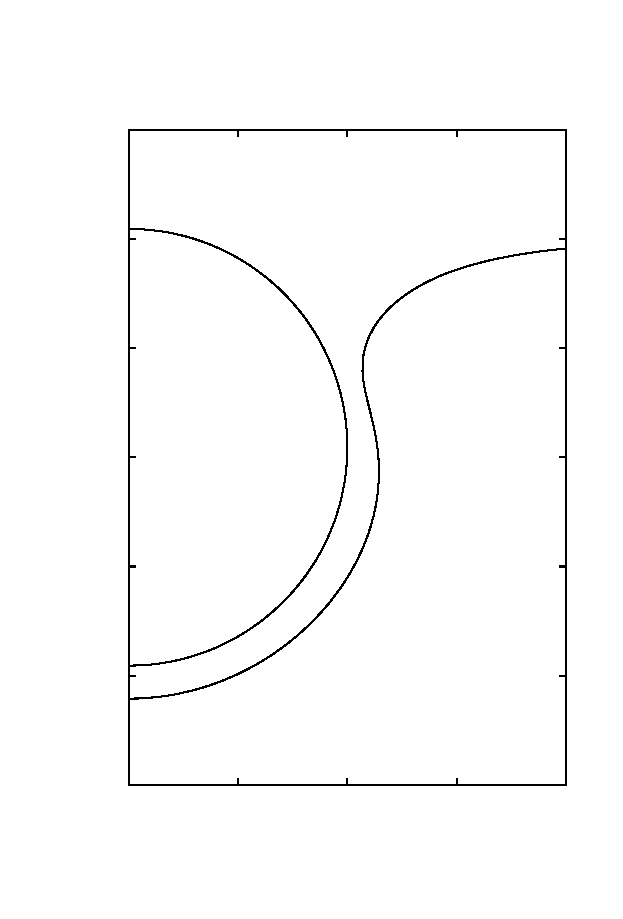
\includegraphics{float4}}%
    \gplfronttext
  \end{picture}%
\endgroup
}
        \caption{}
        \label{fig:float4}
      \end{subfigure}

      \begin{subfigure}[b]{0.9\textwidth}
        \resizebox{\textwidth}{!}{\normalsize % GNUPLOT: LaTeX picture with Postscript
\begingroup
  \makeatletter
  \providecommand\color[2][]{%
    \GenericError{(gnuplot) \space\space\space\@spaces}{%
      Package color not loaded in conjunction with
      terminal option `colourtext'%
    }{See the gnuplot documentation for explanation.%
    }{Either use 'blacktext' in gnuplot or load the package
      color.sty in LaTeX.}%
    \renewcommand\color[2][]{}%
  }%
  \providecommand\includegraphics[2][]{%
    \GenericError{(gnuplot) \space\space\space\@spaces}{%
      Package graphicx or graphics not loaded%
    }{See the gnuplot documentation for explanation.%
    }{The gnuplot epslatex terminal needs graphicx.sty or graphics.sty.}%
    \renewcommand\includegraphics[2][]{}%
  }%
  \providecommand\rotatebox[2]{#2}%
  \@ifundefined{ifGPcolor}{%
    \newif\ifGPcolor
    \GPcolorfalse
  }{}%
  \@ifundefined{ifGPblacktext}{%
    \newif\ifGPblacktext
    \GPblacktexttrue
  }{}%
  % define a \g@addto@macro without @ in the name:
  \let\gplgaddtomacro\g@addto@macro
  % define empty templates for all commands taking text:
  \gdef\gplbacktext{}%
  \gdef\gplfronttext{}%
  \makeatother
  \ifGPblacktext
    % no textcolor at all
    \def\colorrgb#1{}%
    \def\colorgray#1{}%
  \else
    % gray or color?
    \ifGPcolor
      \def\colorrgb#1{\color[rgb]{#1}}%
      \def\colorgray#1{\color[gray]{#1}}%
      \expandafter\def\csname LTw\endcsname{\color{white}}%
      \expandafter\def\csname LTb\endcsname{\color{black}}%
      \expandafter\def\csname LTa\endcsname{\color{black}}%
      \expandafter\def\csname LT0\endcsname{\color[rgb]{1,0,0}}%
      \expandafter\def\csname LT1\endcsname{\color[rgb]{0,1,0}}%
      \expandafter\def\csname LT2\endcsname{\color[rgb]{0,0,1}}%
      \expandafter\def\csname LT3\endcsname{\color[rgb]{1,0,1}}%
      \expandafter\def\csname LT4\endcsname{\color[rgb]{0,1,1}}%
      \expandafter\def\csname LT5\endcsname{\color[rgb]{1,1,0}}%
      \expandafter\def\csname LT6\endcsname{\color[rgb]{0,0,0}}%
      \expandafter\def\csname LT7\endcsname{\color[rgb]{1,0.3,0}}%
      \expandafter\def\csname LT8\endcsname{\color[rgb]{0.5,0.5,0.5}}%
    \else
      % gray
      \def\colorrgb#1{\color{black}}%
      \def\colorgray#1{\color[gray]{#1}}%
      \expandafter\def\csname LTw\endcsname{\color{white}}%
      \expandafter\def\csname LTb\endcsname{\color{black}}%
      \expandafter\def\csname LTa\endcsname{\color{black}}%
      \expandafter\def\csname LT0\endcsname{\color{black}}%
      \expandafter\def\csname LT1\endcsname{\color{black}}%
      \expandafter\def\csname LT2\endcsname{\color{black}}%
      \expandafter\def\csname LT3\endcsname{\color{black}}%
      \expandafter\def\csname LT4\endcsname{\color{black}}%
      \expandafter\def\csname LT5\endcsname{\color{black}}%
      \expandafter\def\csname LT6\endcsname{\color{black}}%
      \expandafter\def\csname LT7\endcsname{\color{black}}%
      \expandafter\def\csname LT8\endcsname{\color{black}}%
    \fi
  \fi
    \setlength{\unitlength}{0.0500bp}%
    \ifx\gptboxheight\undefined%
      \newlength{\gptboxheight}%
      \newlength{\gptboxwidth}%
      \newsavebox{\gptboxtext}%
    \fi%
    \setlength{\fboxrule}{0.5pt}%
    \setlength{\fboxsep}{1pt}%
\begin{picture}(7200.00,5040.00)%
    \gplgaddtomacro\gplbacktext{%
      \csname LTb\endcsname%
      \put(946,704){\makebox(0,0)[r]{\strut{}$0.1$}}%
      \put(946,1383){\makebox(0,0)[r]{\strut{}$0.12$}}%
      \put(946,2061){\makebox(0,0)[r]{\strut{}$0.14$}}%
      \put(946,2740){\makebox(0,0)[r]{\strut{}$0.16$}}%
      \put(946,3418){\makebox(0,0)[r]{\strut{}$0.18$}}%
      \put(946,4097){\makebox(0,0)[r]{\strut{}$0.2$}}%
      \put(946,4775){\makebox(0,0)[r]{\strut{}$0.22$}}%
      \put(1078,484){\makebox(0,0){\strut{}$\pi / 2$}}%
      \put(3941,484){\makebox(0,0){\strut{}$3 \pi / 4$}}%
      \put(6803,484){\makebox(0,0){\strut{}$\pi$}}%
    }%
    \gplgaddtomacro\gplfronttext{%
      \csname LTb\endcsname%
      \put(176,2739){\rotatebox{-270}{\makebox(0,0){\strut{}$\delta / a$}}}%
      \put(3940,154){\makebox(0,0){\strut{}$\theta$}}%
      \csname LTb\endcsname%
      \put(5816,1537){\makebox(0,0)[r]{\strut{}$\Bo = 1$, $D = 3.4$}}%
      \csname LTb\endcsname%
      \put(5816,1317){\makebox(0,0)[r]{\strut{}$\Bo = 1.5$, $D = 2.8$}}%
      \csname LTb\endcsname%
      \put(5816,1097){\makebox(0,0)[r]{\strut{}$\Bo = 2.5$, $D = 2.2$}}%
      \csname LTb\endcsname%
      \put(5816,877){\makebox(0,0)[r]{\strut{}$\Bo = 3.5$, $D = 2$}}%
    }%
    \gplbacktext
    \put(0,0){\includegraphics{film_profiles}}%
    \gplfronttext
  \end{picture}%
\endgroup
}
        \caption{}
        \label{fig:film_prof}
      \end{subfigure}
      \caption{a) to d) The final equilibrium configuration of the simulations listed in table~\ref{tab:film_sims}. In each example, the film constricts at approximately $\theta = \pi / 2$, just before the interface transitions into the meniscus profile. e) Film thickness as a function of $\theta$. The film thickness can be seen to vary up to about 50\%.}\label{fig:float_films}
    \end{figure}

As can be seen in figures~\ref{fig:float1} to~\ref{fig:float4}, the film is seen to contract at its periphery. This agrees with previous experimental observations \citep{Hartland68} where it has been noted that the film constricts at it's periphery, just inside the point where it transitions to the meniscus profile. This constriction is predicted by the theoretical model of \citep{Jones78} as a consequence of pressure gradients in the film as a consequence of the change in curvature of the interface at the film periphery. 

Additionally, the point where the film transitions to the meniscus occurs at a polar angle of $\theta \approx \pi / 2$. This is the first point of agreement with the modified static model. Differentiating of equation~\ref{equ:mod_non_dim} with respect to $\theta_{\text{c}}$ and setting $\partial D / \partial \theta_{\text{c}} = 0$ gives a solution of $\theta_{\text{c}} = \pi / 2$ (other solutions may exist but cannot be extracted due to the unavailability for a closed expression for $\partial z_{\text{c}} / \partial \theta_{\text{c}}$). Hence, there is a (at least a local) maximum in maximum value of $D$ for which floating can occur at $\theta_{\text{c}} = \pi / 2$. Since the chosen simulations are close to the transition, it is to be expected that they have an equilibrium configuration which gives this maximum upward force.

Figure~\ref{fig:film_prof} shows the film thickness as a function of $\theta$ for the different simulations. It can be seen that, unlike in the modified static model, the film has a variable thickness which can vary by up to 50\%. Therefore, to compare these simulations with the results from the static model, the mean thickness of the film, weighted by the radial coordinate, has been calculated. The reason for weighting by the radial coordinate is because the axisymmtric geometry means, for a given film thickness, there is a greater volume of fluid at a larger radius. The weighted mean thicknesses $\bar{\delta}$ and their corresponding value of $\Delta$ are given in table~\ref{tab:film_sims}. Figure~\ref{fig:float_trans} shows the predicted transitions for these values of $\Delta$ compared to the results from the BIM. It can be seen that all values of $\Delta$ reproduce the observed transition for $\Bo \geq 4$ and that as $\Delta$ decreases then the lowest value of $\Bo$ at which there is agreement becomes smaller; for $\Delta = 1.339$ there is agreement for $\Bo \geq 1.5$. For smaller $\Bo$, the static model predicts the transition to be at larger values of $D$ than the BIM model. This discrepancy is most likely explained by the fact that as $\Bo$ decreases, the amount of variation in film thickness increases (figure~\ref{fig:film_prof}) so the assumption of constant film thickness in the static model begins to no longer be valid. However, regardless, the modified static model still does a very good job of predicting the transition observed in the BIM, compared to the original static model (see figure~\ref{fig:zoom_regime}).

    \begin{figure}
      \centering
      \begin{subfigure}[b]{0.45\textwidth}
        \resizebox{\textwidth}{!}{\Large % GNUPLOT: LaTeX picture with Postscript
\begingroup
  \makeatletter
  \providecommand\color[2][]{%
    \GenericError{(gnuplot) \space\space\space\@spaces}{%
      Package color not loaded in conjunction with
      terminal option `colourtext'%
    }{See the gnuplot documentation for explanation.%
    }{Either use 'blacktext' in gnuplot or load the package
      color.sty in LaTeX.}%
    \renewcommand\color[2][]{}%
  }%
  \providecommand\includegraphics[2][]{%
    \GenericError{(gnuplot) \space\space\space\@spaces}{%
      Package graphicx or graphics not loaded%
    }{See the gnuplot documentation for explanation.%
    }{The gnuplot epslatex terminal needs graphicx.sty or graphics.sty.}%
    \renewcommand\includegraphics[2][]{}%
  }%
  \providecommand\rotatebox[2]{#2}%
  \@ifundefined{ifGPcolor}{%
    \newif\ifGPcolor
    \GPcolorfalse
  }{}%
  \@ifundefined{ifGPblacktext}{%
    \newif\ifGPblacktext
    \GPblacktexttrue
  }{}%
  % define a \g@addto@macro without @ in the name:
  \let\gplgaddtomacro\g@addto@macro
  % define empty templates for all commands taking text:
  \gdef\gplbacktext{}%
  \gdef\gplfronttext{}%
  \makeatother
  \ifGPblacktext
    % no textcolor at all
    \def\colorrgb#1{}%
    \def\colorgray#1{}%
  \else
    % gray or color?
    \ifGPcolor
      \def\colorrgb#1{\color[rgb]{#1}}%
      \def\colorgray#1{\color[gray]{#1}}%
      \expandafter\def\csname LTw\endcsname{\color{white}}%
      \expandafter\def\csname LTb\endcsname{\color{black}}%
      \expandafter\def\csname LTa\endcsname{\color{black}}%
      \expandafter\def\csname LT0\endcsname{\color[rgb]{1,0,0}}%
      \expandafter\def\csname LT1\endcsname{\color[rgb]{0,1,0}}%
      \expandafter\def\csname LT2\endcsname{\color[rgb]{0,0,1}}%
      \expandafter\def\csname LT3\endcsname{\color[rgb]{1,0,1}}%
      \expandafter\def\csname LT4\endcsname{\color[rgb]{0,1,1}}%
      \expandafter\def\csname LT5\endcsname{\color[rgb]{1,1,0}}%
      \expandafter\def\csname LT6\endcsname{\color[rgb]{0,0,0}}%
      \expandafter\def\csname LT7\endcsname{\color[rgb]{1,0.3,0}}%
      \expandafter\def\csname LT8\endcsname{\color[rgb]{0.5,0.5,0.5}}%
    \else
      % gray
      \def\colorrgb#1{\color{black}}%
      \def\colorgray#1{\color[gray]{#1}}%
      \expandafter\def\csname LTw\endcsname{\color{white}}%
      \expandafter\def\csname LTb\endcsname{\color{black}}%
      \expandafter\def\csname LTa\endcsname{\color{black}}%
      \expandafter\def\csname LT0\endcsname{\color{black}}%
      \expandafter\def\csname LT1\endcsname{\color{black}}%
      \expandafter\def\csname LT2\endcsname{\color{black}}%
      \expandafter\def\csname LT3\endcsname{\color{black}}%
      \expandafter\def\csname LT4\endcsname{\color{black}}%
      \expandafter\def\csname LT5\endcsname{\color{black}}%
      \expandafter\def\csname LT6\endcsname{\color{black}}%
      \expandafter\def\csname LT7\endcsname{\color{black}}%
      \expandafter\def\csname LT8\endcsname{\color{black}}%
    \fi
  \fi
    \setlength{\unitlength}{0.0500bp}%
    \ifx\gptboxheight\undefined%
      \newlength{\gptboxheight}%
      \newlength{\gptboxwidth}%
      \newsavebox{\gptboxtext}%
    \fi%
    \setlength{\fboxrule}{0.5pt}%
    \setlength{\fboxsep}{1pt}%
\begin{picture}(7200.00,5040.00)%
    \gplgaddtomacro\gplbacktext{%
      \csname LTb\endcsname%
      \put(550,704){\makebox(0,0)[r]{\strut{}$0$}}%
      \put(550,1439){\makebox(0,0)[r]{\strut{}$1$}}%
      \put(550,2174){\makebox(0,0)[r]{\strut{}$2$}}%
      \put(550,2909){\makebox(0,0)[r]{\strut{}$3$}}%
      \put(550,3644){\makebox(0,0)[r]{\strut{}$4$}}%
      \put(550,4379){\makebox(0,0)[r]{\strut{}$5$}}%
      \put(682,484){\makebox(0,0){\strut{}$0$}}%
      \put(1906,484){\makebox(0,0){\strut{}$1$}}%
      \put(3130,484){\makebox(0,0){\strut{}$2$}}%
      \put(4355,484){\makebox(0,0){\strut{}$3$}}%
      \put(5579,484){\makebox(0,0){\strut{}$4$}}%
      \put(6803,484){\makebox(0,0){\strut{}$5$}}%
    }%
    \gplgaddtomacro\gplfronttext{%
      \csname LTb\endcsname%
      \put(176,2541){\rotatebox{-270}{\makebox(0,0){\strut{}$D$}}}%
      \put(3742,154){\makebox(0,0){\strut{}$\Bo$}}%
      \put(3742,4709){\makebox(0,0){\strut{}$\Delta = 1.381$}}%
      \csname LTb\endcsname%
      \put(5816,4206){\makebox(0,0)[r]{\strut{}Floating}}%
      \csname LTb\endcsname%
      \put(5816,3986){\makebox(0,0)[r]{\strut{}Sinking}}%
    }%
    \gplbacktext
    \put(0,0){\includegraphics{float1_trans}}%
    \gplfronttext
  \end{picture}%
\endgroup
}
        \caption{}
        \label{fig:float1}
      \end{subfigure}
      ~
      \begin{subfigure}[b]{0.45\textwidth}
        \resizebox{\textwidth}{!}{\Large % GNUPLOT: LaTeX picture with Postscript
\begingroup
  \makeatletter
  \providecommand\color[2][]{%
    \GenericError{(gnuplot) \space\space\space\@spaces}{%
      Package color not loaded in conjunction with
      terminal option `colourtext'%
    }{See the gnuplot documentation for explanation.%
    }{Either use 'blacktext' in gnuplot or load the package
      color.sty in LaTeX.}%
    \renewcommand\color[2][]{}%
  }%
  \providecommand\includegraphics[2][]{%
    \GenericError{(gnuplot) \space\space\space\@spaces}{%
      Package graphicx or graphics not loaded%
    }{See the gnuplot documentation for explanation.%
    }{The gnuplot epslatex terminal needs graphicx.sty or graphics.sty.}%
    \renewcommand\includegraphics[2][]{}%
  }%
  \providecommand\rotatebox[2]{#2}%
  \@ifundefined{ifGPcolor}{%
    \newif\ifGPcolor
    \GPcolorfalse
  }{}%
  \@ifundefined{ifGPblacktext}{%
    \newif\ifGPblacktext
    \GPblacktexttrue
  }{}%
  % define a \g@addto@macro without @ in the name:
  \let\gplgaddtomacro\g@addto@macro
  % define empty templates for all commands taking text:
  \gdef\gplbacktext{}%
  \gdef\gplfronttext{}%
  \makeatother
  \ifGPblacktext
    % no textcolor at all
    \def\colorrgb#1{}%
    \def\colorgray#1{}%
  \else
    % gray or color?
    \ifGPcolor
      \def\colorrgb#1{\color[rgb]{#1}}%
      \def\colorgray#1{\color[gray]{#1}}%
      \expandafter\def\csname LTw\endcsname{\color{white}}%
      \expandafter\def\csname LTb\endcsname{\color{black}}%
      \expandafter\def\csname LTa\endcsname{\color{black}}%
      \expandafter\def\csname LT0\endcsname{\color[rgb]{1,0,0}}%
      \expandafter\def\csname LT1\endcsname{\color[rgb]{0,1,0}}%
      \expandafter\def\csname LT2\endcsname{\color[rgb]{0,0,1}}%
      \expandafter\def\csname LT3\endcsname{\color[rgb]{1,0,1}}%
      \expandafter\def\csname LT4\endcsname{\color[rgb]{0,1,1}}%
      \expandafter\def\csname LT5\endcsname{\color[rgb]{1,1,0}}%
      \expandafter\def\csname LT6\endcsname{\color[rgb]{0,0,0}}%
      \expandafter\def\csname LT7\endcsname{\color[rgb]{1,0.3,0}}%
      \expandafter\def\csname LT8\endcsname{\color[rgb]{0.5,0.5,0.5}}%
    \else
      % gray
      \def\colorrgb#1{\color{black}}%
      \def\colorgray#1{\color[gray]{#1}}%
      \expandafter\def\csname LTw\endcsname{\color{white}}%
      \expandafter\def\csname LTb\endcsname{\color{black}}%
      \expandafter\def\csname LTa\endcsname{\color{black}}%
      \expandafter\def\csname LT0\endcsname{\color{black}}%
      \expandafter\def\csname LT1\endcsname{\color{black}}%
      \expandafter\def\csname LT2\endcsname{\color{black}}%
      \expandafter\def\csname LT3\endcsname{\color{black}}%
      \expandafter\def\csname LT4\endcsname{\color{black}}%
      \expandafter\def\csname LT5\endcsname{\color{black}}%
      \expandafter\def\csname LT6\endcsname{\color{black}}%
      \expandafter\def\csname LT7\endcsname{\color{black}}%
      \expandafter\def\csname LT8\endcsname{\color{black}}%
    \fi
  \fi
    \setlength{\unitlength}{0.0500bp}%
    \ifx\gptboxheight\undefined%
      \newlength{\gptboxheight}%
      \newlength{\gptboxwidth}%
      \newsavebox{\gptboxtext}%
    \fi%
    \setlength{\fboxrule}{0.5pt}%
    \setlength{\fboxsep}{1pt}%
\begin{picture}(7200.00,5040.00)%
    \gplgaddtomacro\gplbacktext{%
      \csname LTb\endcsname%
      \put(550,704){\makebox(0,0)[r]{\strut{}$0$}}%
      \put(550,1439){\makebox(0,0)[r]{\strut{}$1$}}%
      \put(550,2174){\makebox(0,0)[r]{\strut{}$2$}}%
      \put(550,2909){\makebox(0,0)[r]{\strut{}$3$}}%
      \put(550,3644){\makebox(0,0)[r]{\strut{}$4$}}%
      \put(550,4379){\makebox(0,0)[r]{\strut{}$5$}}%
      \put(682,484){\makebox(0,0){\strut{}$0$}}%
      \put(1906,484){\makebox(0,0){\strut{}$1$}}%
      \put(3130,484){\makebox(0,0){\strut{}$2$}}%
      \put(4355,484){\makebox(0,0){\strut{}$3$}}%
      \put(5579,484){\makebox(0,0){\strut{}$4$}}%
      \put(6803,484){\makebox(0,0){\strut{}$5$}}%
    }%
    \gplgaddtomacro\gplfronttext{%
      \csname LTb\endcsname%
      \put(176,2541){\rotatebox{-270}{\makebox(0,0){\strut{}$D$}}}%
      \put(3742,154){\makebox(0,0){\strut{}$\Bo$}}%
      \put(3742,4709){\makebox(0,0){\strut{}$\Delta = 1.371$}}%
      \csname LTb\endcsname%
      \put(5816,4206){\makebox(0,0)[r]{\strut{}Floating}}%
      \csname LTb\endcsname%
      \put(5816,3986){\makebox(0,0)[r]{\strut{}Sinking}}%
    }%
    \gplbacktext
    \put(0,0){\includegraphics{../../Programming/sinking_bim_write_up/trunk/float2_trans}}%
    \gplfronttext
  \end{picture}%
\endgroup
}
        \caption{}
        \label{fig:float2}
      \end{subfigure}
      
      \begin{subfigure}[b]{0.45\textwidth}
        \resizebox{\textwidth}{!}{\Large % GNUPLOT: LaTeX picture with Postscript
\begingroup
  \makeatletter
  \providecommand\color[2][]{%
    \GenericError{(gnuplot) \space\space\space\@spaces}{%
      Package color not loaded in conjunction with
      terminal option `colourtext'%
    }{See the gnuplot documentation for explanation.%
    }{Either use 'blacktext' in gnuplot or load the package
      color.sty in LaTeX.}%
    \renewcommand\color[2][]{}%
  }%
  \providecommand\includegraphics[2][]{%
    \GenericError{(gnuplot) \space\space\space\@spaces}{%
      Package graphicx or graphics not loaded%
    }{See the gnuplot documentation for explanation.%
    }{The gnuplot epslatex terminal needs graphicx.sty or graphics.sty.}%
    \renewcommand\includegraphics[2][]{}%
  }%
  \providecommand\rotatebox[2]{#2}%
  \@ifundefined{ifGPcolor}{%
    \newif\ifGPcolor
    \GPcolorfalse
  }{}%
  \@ifundefined{ifGPblacktext}{%
    \newif\ifGPblacktext
    \GPblacktexttrue
  }{}%
  % define a \g@addto@macro without @ in the name:
  \let\gplgaddtomacro\g@addto@macro
  % define empty templates for all commands taking text:
  \gdef\gplbacktext{}%
  \gdef\gplfronttext{}%
  \makeatother
  \ifGPblacktext
    % no textcolor at all
    \def\colorrgb#1{}%
    \def\colorgray#1{}%
  \else
    % gray or color?
    \ifGPcolor
      \def\colorrgb#1{\color[rgb]{#1}}%
      \def\colorgray#1{\color[gray]{#1}}%
      \expandafter\def\csname LTw\endcsname{\color{white}}%
      \expandafter\def\csname LTb\endcsname{\color{black}}%
      \expandafter\def\csname LTa\endcsname{\color{black}}%
      \expandafter\def\csname LT0\endcsname{\color[rgb]{1,0,0}}%
      \expandafter\def\csname LT1\endcsname{\color[rgb]{0,1,0}}%
      \expandafter\def\csname LT2\endcsname{\color[rgb]{0,0,1}}%
      \expandafter\def\csname LT3\endcsname{\color[rgb]{1,0,1}}%
      \expandafter\def\csname LT4\endcsname{\color[rgb]{0,1,1}}%
      \expandafter\def\csname LT5\endcsname{\color[rgb]{1,1,0}}%
      \expandafter\def\csname LT6\endcsname{\color[rgb]{0,0,0}}%
      \expandafter\def\csname LT7\endcsname{\color[rgb]{1,0.3,0}}%
      \expandafter\def\csname LT8\endcsname{\color[rgb]{0.5,0.5,0.5}}%
    \else
      % gray
      \def\colorrgb#1{\color{black}}%
      \def\colorgray#1{\color[gray]{#1}}%
      \expandafter\def\csname LTw\endcsname{\color{white}}%
      \expandafter\def\csname LTb\endcsname{\color{black}}%
      \expandafter\def\csname LTa\endcsname{\color{black}}%
      \expandafter\def\csname LT0\endcsname{\color{black}}%
      \expandafter\def\csname LT1\endcsname{\color{black}}%
      \expandafter\def\csname LT2\endcsname{\color{black}}%
      \expandafter\def\csname LT3\endcsname{\color{black}}%
      \expandafter\def\csname LT4\endcsname{\color{black}}%
      \expandafter\def\csname LT5\endcsname{\color{black}}%
      \expandafter\def\csname LT6\endcsname{\color{black}}%
      \expandafter\def\csname LT7\endcsname{\color{black}}%
      \expandafter\def\csname LT8\endcsname{\color{black}}%
    \fi
  \fi
    \setlength{\unitlength}{0.0500bp}%
    \ifx\gptboxheight\undefined%
      \newlength{\gptboxheight}%
      \newlength{\gptboxwidth}%
      \newsavebox{\gptboxtext}%
    \fi%
    \setlength{\fboxrule}{0.5pt}%
    \setlength{\fboxsep}{1pt}%
\begin{picture}(7200.00,5040.00)%
    \gplgaddtomacro\gplbacktext{%
      \csname LTb\endcsname%
      \put(550,704){\makebox(0,0)[r]{\strut{}$0$}}%
      \put(550,1439){\makebox(0,0)[r]{\strut{}$1$}}%
      \put(550,2174){\makebox(0,0)[r]{\strut{}$2$}}%
      \put(550,2909){\makebox(0,0)[r]{\strut{}$3$}}%
      \put(550,3644){\makebox(0,0)[r]{\strut{}$4$}}%
      \put(550,4379){\makebox(0,0)[r]{\strut{}$5$}}%
      \put(682,484){\makebox(0,0){\strut{}$0$}}%
      \put(1906,484){\makebox(0,0){\strut{}$1$}}%
      \put(3130,484){\makebox(0,0){\strut{}$2$}}%
      \put(4355,484){\makebox(0,0){\strut{}$3$}}%
      \put(5579,484){\makebox(0,0){\strut{}$4$}}%
      \put(6803,484){\makebox(0,0){\strut{}$5$}}%
    }%
    \gplgaddtomacro\gplfronttext{%
      \csname LTb\endcsname%
      \put(176,2541){\rotatebox{-270}{\makebox(0,0){\strut{}$D$}}}%
      \put(3742,154){\makebox(0,0){\strut{}$\Bo$}}%
      \put(3742,4709){\makebox(0,0){\strut{}$\Delta = 1.346$}}%
      \csname LTb\endcsname%
      \put(5816,4206){\makebox(0,0)[r]{\strut{}Floating}}%
      \csname LTb\endcsname%
      \put(5816,3986){\makebox(0,0)[r]{\strut{}Sinking}}%
    }%
    \gplbacktext
    \put(0,0){\includegraphics{../../Programming/sinking_bim_write_up/trunk/float3_trans}}%
    \gplfronttext
  \end{picture}%
\endgroup
}
        \caption{}
        \label{fig:float3}
      \end{subfigure}
      ~
      \begin{subfigure}[b]{0.45\textwidth}
        \resizebox{\textwidth}{!}{\Large % GNUPLOT: LaTeX picture with Postscript
\begingroup
  \makeatletter
  \providecommand\color[2][]{%
    \GenericError{(gnuplot) \space\space\space\@spaces}{%
      Package color not loaded in conjunction with
      terminal option `colourtext'%
    }{See the gnuplot documentation for explanation.%
    }{Either use 'blacktext' in gnuplot or load the package
      color.sty in LaTeX.}%
    \renewcommand\color[2][]{}%
  }%
  \providecommand\includegraphics[2][]{%
    \GenericError{(gnuplot) \space\space\space\@spaces}{%
      Package graphicx or graphics not loaded%
    }{See the gnuplot documentation for explanation.%
    }{The gnuplot epslatex terminal needs graphicx.sty or graphics.sty.}%
    \renewcommand\includegraphics[2][]{}%
  }%
  \providecommand\rotatebox[2]{#2}%
  \@ifundefined{ifGPcolor}{%
    \newif\ifGPcolor
    \GPcolorfalse
  }{}%
  \@ifundefined{ifGPblacktext}{%
    \newif\ifGPblacktext
    \GPblacktexttrue
  }{}%
  % define a \g@addto@macro without @ in the name:
  \let\gplgaddtomacro\g@addto@macro
  % define empty templates for all commands taking text:
  \gdef\gplbacktext{}%
  \gdef\gplfronttext{}%
  \makeatother
  \ifGPblacktext
    % no textcolor at all
    \def\colorrgb#1{}%
    \def\colorgray#1{}%
  \else
    % gray or color?
    \ifGPcolor
      \def\colorrgb#1{\color[rgb]{#1}}%
      \def\colorgray#1{\color[gray]{#1}}%
      \expandafter\def\csname LTw\endcsname{\color{white}}%
      \expandafter\def\csname LTb\endcsname{\color{black}}%
      \expandafter\def\csname LTa\endcsname{\color{black}}%
      \expandafter\def\csname LT0\endcsname{\color[rgb]{1,0,0}}%
      \expandafter\def\csname LT1\endcsname{\color[rgb]{0,1,0}}%
      \expandafter\def\csname LT2\endcsname{\color[rgb]{0,0,1}}%
      \expandafter\def\csname LT3\endcsname{\color[rgb]{1,0,1}}%
      \expandafter\def\csname LT4\endcsname{\color[rgb]{0,1,1}}%
      \expandafter\def\csname LT5\endcsname{\color[rgb]{1,1,0}}%
      \expandafter\def\csname LT6\endcsname{\color[rgb]{0,0,0}}%
      \expandafter\def\csname LT7\endcsname{\color[rgb]{1,0.3,0}}%
      \expandafter\def\csname LT8\endcsname{\color[rgb]{0.5,0.5,0.5}}%
    \else
      % gray
      \def\colorrgb#1{\color{black}}%
      \def\colorgray#1{\color[gray]{#1}}%
      \expandafter\def\csname LTw\endcsname{\color{white}}%
      \expandafter\def\csname LTb\endcsname{\color{black}}%
      \expandafter\def\csname LTa\endcsname{\color{black}}%
      \expandafter\def\csname LT0\endcsname{\color{black}}%
      \expandafter\def\csname LT1\endcsname{\color{black}}%
      \expandafter\def\csname LT2\endcsname{\color{black}}%
      \expandafter\def\csname LT3\endcsname{\color{black}}%
      \expandafter\def\csname LT4\endcsname{\color{black}}%
      \expandafter\def\csname LT5\endcsname{\color{black}}%
      \expandafter\def\csname LT6\endcsname{\color{black}}%
      \expandafter\def\csname LT7\endcsname{\color{black}}%
      \expandafter\def\csname LT8\endcsname{\color{black}}%
    \fi
  \fi
    \setlength{\unitlength}{0.0500bp}%
    \ifx\gptboxheight\undefined%
      \newlength{\gptboxheight}%
      \newlength{\gptboxwidth}%
      \newsavebox{\gptboxtext}%
    \fi%
    \setlength{\fboxrule}{0.5pt}%
    \setlength{\fboxsep}{1pt}%
\begin{picture}(7200.00,5040.00)%
    \gplgaddtomacro\gplbacktext{%
      \csname LTb\endcsname%
      \put(550,704){\makebox(0,0)[r]{\strut{}$0$}}%
      \put(550,1439){\makebox(0,0)[r]{\strut{}$1$}}%
      \put(550,2174){\makebox(0,0)[r]{\strut{}$2$}}%
      \put(550,2909){\makebox(0,0)[r]{\strut{}$3$}}%
      \put(550,3644){\makebox(0,0)[r]{\strut{}$4$}}%
      \put(550,4379){\makebox(0,0)[r]{\strut{}$5$}}%
      \put(682,484){\makebox(0,0){\strut{}$0$}}%
      \put(1906,484){\makebox(0,0){\strut{}$1$}}%
      \put(3130,484){\makebox(0,0){\strut{}$2$}}%
      \put(4355,484){\makebox(0,0){\strut{}$3$}}%
      \put(5579,484){\makebox(0,0){\strut{}$4$}}%
      \put(6803,484){\makebox(0,0){\strut{}$5$}}%
    }%
    \gplgaddtomacro\gplfronttext{%
      \csname LTb\endcsname%
      \put(176,2541){\rotatebox{-270}{\makebox(0,0){\strut{}$D$}}}%
      \put(3742,154){\makebox(0,0){\strut{}$\Bo$}}%
      \put(3742,4709){\makebox(0,0){\strut{}$\Delta = 1.339$}}%
      \csname LTb\endcsname%
      \put(5816,4206){\makebox(0,0)[r]{\strut{}Floating}}%
      \csname LTb\endcsname%
      \put(5816,3986){\makebox(0,0)[r]{\strut{}Sinking}}%
    }%
    \gplbacktext
    \put(0,0){\includegraphics{float4_trans}}%
    \gplfronttext
  \end{picture}%
\endgroup
}
        \caption{}
        \label{fig:float4}
      \end{subfigure}
      \caption{Predicted transitions based on the mean thickness of each film. }\label{fig:float_trans}
    \end{figure}

\subsection{Equilibrium Floating Position}
\label{subsec:dis_float_pos}

As figure~\ref{fig:fin_pos_viscos} shows, the equilibrium position of a floating sphere is independent of $\lambda$. This is an intuitive result since viscosity is only relevant for situations where fluid is moving, and floating is a static phenomenon. It is also found that as $\Bo \to 0$, the dependence of $z_{\text{eq}}$ on $D$ vanishes. This is because in this limit, the gravitational forces acting to deform the interface are significantly smaller than the restorative IFT forces meaning it is very difficult to deform the fluid interface. This is why $z_{\text{eq}} \to 1$ in this limit as this corresponds to the sphere sitting on top of a flat, undeformed interface. In the other limit ($\Bo to infty$) it is only possible to consider the case $D = 1$, since the sphere sinks for all other values of $D$. Here, $z_{\text{eq}}$ is observed to tend to the constant value of $-0.32$. That the equilibrium depth of the sphere is independent of the Bond number here is predicted by the modified static model described in section~\ref{subsubsec:mod_stat_mod}, since taking the limit of equation~\ref{equ:mod_non_dim} as $\Bo \to \infty$ and setting $D = 1$ gives

\begin{equation}
\label{equ:bo_to_infty}
z_{\text{c}} = \frac{\Delta^{1/2} (2 + 3 \cos \theta_{\text{c}} - \cos^{3} \theta_{\text{c}})}{3 \sin^{2} \theta_{\text{c}}}.
\end{equation}

Equation~\ref{equ:bo_to_infty} is independent of $\Bo$ so the equilibrium position of the sphere $z_{\text{eq}} = z_{\text{c}} - \cos \theta_{\text{c}}$ is also. 

\subsection{Entrained Volume}
\label{subsec:dis_ent_vol}

Figures~\ref{fig:mdr_snap} and~\ref{fig:viscos_snap} show that below a critical value of $\Bo$, $V \sim \ln \Bo$ at a fixed $D$ and $\lambda$. This result can be compared that obtained by \citet{Pitois99} who performed experiments where steel or glass beads were dropped onto the interface between PDMS oil and water. They found that the volume of the entrained upper phase fluid was independent of $\lambda$ (although in their experiments $10^{-9} \leq \lambda \leq 10^{-10}$) and $V \sim \ln(D \Bo)$. To compare to this study, the data from figure~\ref{fig:viscos_snap} has been replotted with $\ln(D \Bo)$ on the x-axis (figure~\ref{fig:viscos_snap_DBo}). As can be seen, this has the effect of shifting the curves along the x-axis by an amount $\ln D$. It can be seen that at $\ln(D \Bo) \approx 1$, then all of the curves for different values of $D$ are coincident. However, this is generally not true. Hence the conclusion of \citet{Pitois99} that $V \sim \ln(D \Bo)$ is only valid for $\ln(D \Bo) \to 1$ from above. 

    \begin{figure}
      \centering
      \begin{subfigure}[b]{0.45\textwidth}
        \resizebox{\textwidth}{!}{\Large % GNUPLOT: LaTeX picture with Postscript
\begingroup
  \makeatletter
  \providecommand\color[2][]{%
    \GenericError{(gnuplot) \space\space\space\@spaces}{%
      Package color not loaded in conjunction with
      terminal option `colourtext'%
    }{See the gnuplot documentation for explanation.%
    }{Either use 'blacktext' in gnuplot or load the package
      color.sty in LaTeX.}%
    \renewcommand\color[2][]{}%
  }%
  \providecommand\includegraphics[2][]{%
    \GenericError{(gnuplot) \space\space\space\@spaces}{%
      Package graphicx or graphics not loaded%
    }{See the gnuplot documentation for explanation.%
    }{The gnuplot epslatex terminal needs graphicx.sty or graphics.sty.}%
    \renewcommand\includegraphics[2][]{}%
  }%
  \providecommand\rotatebox[2]{#2}%
  \@ifundefined{ifGPcolor}{%
    \newif\ifGPcolor
    \GPcolorfalse
  }{}%
  \@ifundefined{ifGPblacktext}{%
    \newif\ifGPblacktext
    \GPblacktexttrue
  }{}%
  % define a \g@addto@macro without @ in the name:
  \let\gplgaddtomacro\g@addto@macro
  % define empty templates for all commands taking text:
  \gdef\gplbacktext{}%
  \gdef\gplfronttext{}%
  \makeatother
  \ifGPblacktext
    % no textcolor at all
    \def\colorrgb#1{}%
    \def\colorgray#1{}%
  \else
    % gray or color?
    \ifGPcolor
      \def\colorrgb#1{\color[rgb]{#1}}%
      \def\colorgray#1{\color[gray]{#1}}%
      \expandafter\def\csname LTw\endcsname{\color{white}}%
      \expandafter\def\csname LTb\endcsname{\color{black}}%
      \expandafter\def\csname LTa\endcsname{\color{black}}%
      \expandafter\def\csname LT0\endcsname{\color[rgb]{1,0,0}}%
      \expandafter\def\csname LT1\endcsname{\color[rgb]{0,1,0}}%
      \expandafter\def\csname LT2\endcsname{\color[rgb]{0,0,1}}%
      \expandafter\def\csname LT3\endcsname{\color[rgb]{1,0,1}}%
      \expandafter\def\csname LT4\endcsname{\color[rgb]{0,1,1}}%
      \expandafter\def\csname LT5\endcsname{\color[rgb]{1,1,0}}%
      \expandafter\def\csname LT6\endcsname{\color[rgb]{0,0,0}}%
      \expandafter\def\csname LT7\endcsname{\color[rgb]{1,0.3,0}}%
      \expandafter\def\csname LT8\endcsname{\color[rgb]{0.5,0.5,0.5}}%
    \else
      % gray
      \def\colorrgb#1{\color{black}}%
      \def\colorgray#1{\color[gray]{#1}}%
      \expandafter\def\csname LTw\endcsname{\color{white}}%
      \expandafter\def\csname LTb\endcsname{\color{black}}%
      \expandafter\def\csname LTa\endcsname{\color{black}}%
      \expandafter\def\csname LT0\endcsname{\color{black}}%
      \expandafter\def\csname LT1\endcsname{\color{black}}%
      \expandafter\def\csname LT2\endcsname{\color{black}}%
      \expandafter\def\csname LT3\endcsname{\color{black}}%
      \expandafter\def\csname LT4\endcsname{\color{black}}%
      \expandafter\def\csname LT5\endcsname{\color{black}}%
      \expandafter\def\csname LT6\endcsname{\color{black}}%
      \expandafter\def\csname LT7\endcsname{\color{black}}%
      \expandafter\def\csname LT8\endcsname{\color{black}}%
    \fi
  \fi
    \setlength{\unitlength}{0.0500bp}%
    \ifx\gptboxheight\undefined%
      \newlength{\gptboxheight}%
      \newlength{\gptboxwidth}%
      \newsavebox{\gptboxtext}%
    \fi%
    \setlength{\fboxrule}{0.5pt}%
    \setlength{\fboxsep}{1pt}%
\begin{picture}(7200.00,5040.00)%
    \gplgaddtomacro\gplbacktext{%
      \csname LTb\endcsname%
      \put(682,704){\makebox(0,0)[r]{\strut{}$0$}}%
      \put(682,1112){\makebox(0,0)[r]{\strut{}$2$}}%
      \put(682,1521){\makebox(0,0)[r]{\strut{}$4$}}%
      \put(682,1929){\makebox(0,0)[r]{\strut{}$6$}}%
      \put(682,2337){\makebox(0,0)[r]{\strut{}$8$}}%
      \put(682,2746){\makebox(0,0)[r]{\strut{}$10$}}%
      \put(682,3154){\makebox(0,0)[r]{\strut{}$12$}}%
      \put(682,3562){\makebox(0,0)[r]{\strut{}$14$}}%
      \put(682,3971){\makebox(0,0)[r]{\strut{}$16$}}%
      \put(682,4379){\makebox(0,0)[r]{\strut{}$18$}}%
      \put(814,484){\makebox(0,0){\strut{}$0$}}%
      \put(1670,484){\makebox(0,0){\strut{}$2$}}%
      \put(2525,484){\makebox(0,0){\strut{}$4$}}%
      \put(3381,484){\makebox(0,0){\strut{}$6$}}%
      \put(4236,484){\makebox(0,0){\strut{}$8$}}%
      \put(5092,484){\makebox(0,0){\strut{}$10$}}%
      \put(5947,484){\makebox(0,0){\strut{}$12$}}%
      \put(6803,484){\makebox(0,0){\strut{}$14$}}%
    }%
    \gplgaddtomacro\gplfronttext{%
      \csname LTb\endcsname%
      \put(176,2541){\rotatebox{-270}{\makebox(0,0){\strut{}$V$}}}%
      \put(3808,154){\makebox(0,0){\strut{}$\ln( D \Bo)$}}%
      \put(3808,4709){\makebox(0,0){\strut{}$\lambda = 0.001$}}%
    }%
    \gplbacktext
    \put(0,0){\includegraphics{viscos_rat=001_DBo_pub}}%
    \gplfronttext
  \end{picture}%
\endgroup
}
        \caption{}
        \label{fig:viscos_rat=0.001_DBo}
      \end{subfigure}
      ~
      \begin{subfigure}[b]{0.45\textwidth}
        \resizebox{\textwidth}{!}{\Large % GNUPLOT: LaTeX picture with Postscript
\begingroup
  \makeatletter
  \providecommand\color[2][]{%
    \GenericError{(gnuplot) \space\space\space\@spaces}{%
      Package color not loaded in conjunction with
      terminal option `colourtext'%
    }{See the gnuplot documentation for explanation.%
    }{Either use 'blacktext' in gnuplot or load the package
      color.sty in LaTeX.}%
    \renewcommand\color[2][]{}%
  }%
  \providecommand\includegraphics[2][]{%
    \GenericError{(gnuplot) \space\space\space\@spaces}{%
      Package graphicx or graphics not loaded%
    }{See the gnuplot documentation for explanation.%
    }{The gnuplot epslatex terminal needs graphicx.sty or graphics.sty.}%
    \renewcommand\includegraphics[2][]{}%
  }%
  \providecommand\rotatebox[2]{#2}%
  \@ifundefined{ifGPcolor}{%
    \newif\ifGPcolor
    \GPcolorfalse
  }{}%
  \@ifundefined{ifGPblacktext}{%
    \newif\ifGPblacktext
    \GPblacktexttrue
  }{}%
  % define a \g@addto@macro without @ in the name:
  \let\gplgaddtomacro\g@addto@macro
  % define empty templates for all commands taking text:
  \gdef\gplbacktext{}%
  \gdef\gplfronttext{}%
  \makeatother
  \ifGPblacktext
    % no textcolor at all
    \def\colorrgb#1{}%
    \def\colorgray#1{}%
  \else
    % gray or color?
    \ifGPcolor
      \def\colorrgb#1{\color[rgb]{#1}}%
      \def\colorgray#1{\color[gray]{#1}}%
      \expandafter\def\csname LTw\endcsname{\color{white}}%
      \expandafter\def\csname LTb\endcsname{\color{black}}%
      \expandafter\def\csname LTa\endcsname{\color{black}}%
      \expandafter\def\csname LT0\endcsname{\color[rgb]{1,0,0}}%
      \expandafter\def\csname LT1\endcsname{\color[rgb]{0,1,0}}%
      \expandafter\def\csname LT2\endcsname{\color[rgb]{0,0,1}}%
      \expandafter\def\csname LT3\endcsname{\color[rgb]{1,0,1}}%
      \expandafter\def\csname LT4\endcsname{\color[rgb]{0,1,1}}%
      \expandafter\def\csname LT5\endcsname{\color[rgb]{1,1,0}}%
      \expandafter\def\csname LT6\endcsname{\color[rgb]{0,0,0}}%
      \expandafter\def\csname LT7\endcsname{\color[rgb]{1,0.3,0}}%
      \expandafter\def\csname LT8\endcsname{\color[rgb]{0.5,0.5,0.5}}%
    \else
      % gray
      \def\colorrgb#1{\color{black}}%
      \def\colorgray#1{\color[gray]{#1}}%
      \expandafter\def\csname LTw\endcsname{\color{white}}%
      \expandafter\def\csname LTb\endcsname{\color{black}}%
      \expandafter\def\csname LTa\endcsname{\color{black}}%
      \expandafter\def\csname LT0\endcsname{\color{black}}%
      \expandafter\def\csname LT1\endcsname{\color{black}}%
      \expandafter\def\csname LT2\endcsname{\color{black}}%
      \expandafter\def\csname LT3\endcsname{\color{black}}%
      \expandafter\def\csname LT4\endcsname{\color{black}}%
      \expandafter\def\csname LT5\endcsname{\color{black}}%
      \expandafter\def\csname LT6\endcsname{\color{black}}%
      \expandafter\def\csname LT7\endcsname{\color{black}}%
      \expandafter\def\csname LT8\endcsname{\color{black}}%
    \fi
  \fi
    \setlength{\unitlength}{0.0500bp}%
    \ifx\gptboxheight\undefined%
      \newlength{\gptboxheight}%
      \newlength{\gptboxwidth}%
      \newsavebox{\gptboxtext}%
    \fi%
    \setlength{\fboxrule}{0.5pt}%
    \setlength{\fboxsep}{1pt}%
\begin{picture}(7200.00,5040.00)%
    \gplgaddtomacro\gplbacktext{%
      \csname LTb\endcsname%
      \put(682,704){\makebox(0,0)[r]{\strut{}$0$}}%
      \put(682,1112){\makebox(0,0)[r]{\strut{}$2$}}%
      \put(682,1521){\makebox(0,0)[r]{\strut{}$4$}}%
      \put(682,1929){\makebox(0,0)[r]{\strut{}$6$}}%
      \put(682,2337){\makebox(0,0)[r]{\strut{}$8$}}%
      \put(682,2746){\makebox(0,0)[r]{\strut{}$10$}}%
      \put(682,3154){\makebox(0,0)[r]{\strut{}$12$}}%
      \put(682,3562){\makebox(0,0)[r]{\strut{}$14$}}%
      \put(682,3971){\makebox(0,0)[r]{\strut{}$16$}}%
      \put(682,4379){\makebox(0,0)[r]{\strut{}$18$}}%
      \put(814,484){\makebox(0,0){\strut{}$0$}}%
      \put(1670,484){\makebox(0,0){\strut{}$2$}}%
      \put(2525,484){\makebox(0,0){\strut{}$4$}}%
      \put(3381,484){\makebox(0,0){\strut{}$6$}}%
      \put(4236,484){\makebox(0,0){\strut{}$8$}}%
      \put(5092,484){\makebox(0,0){\strut{}$10$}}%
      \put(5947,484){\makebox(0,0){\strut{}$12$}}%
      \put(6803,484){\makebox(0,0){\strut{}$14$}}%
    }%
    \gplgaddtomacro\gplfronttext{%
      \csname LTb\endcsname%
      \put(176,2541){\rotatebox{-270}{\makebox(0,0){\strut{}$V$}}}%
      \put(3808,154){\makebox(0,0){\strut{}$\ln( D \Bo)$}}%
      \put(3808,4709){\makebox(0,0){\strut{}$\lambda = 0.005$}}%
    }%
    \gplbacktext
    \put(0,0){\includegraphics{viscos_rat=005_DBo_pub}}%
    \gplfronttext
  \end{picture}%
\endgroup
}
        \caption{}
        \label{fig:viscos_rat=0.005_DBo}
      \end{subfigure}
      
      \begin{subfigure}[b]{0.45\textwidth}
        \resizebox{\textwidth}{!}{\Large % GNUPLOT: LaTeX picture with Postscript
\begingroup
  \makeatletter
  \providecommand\color[2][]{%
    \GenericError{(gnuplot) \space\space\space\@spaces}{%
      Package color not loaded in conjunction with
      terminal option `colourtext'%
    }{See the gnuplot documentation for explanation.%
    }{Either use 'blacktext' in gnuplot or load the package
      color.sty in LaTeX.}%
    \renewcommand\color[2][]{}%
  }%
  \providecommand\includegraphics[2][]{%
    \GenericError{(gnuplot) \space\space\space\@spaces}{%
      Package graphicx or graphics not loaded%
    }{See the gnuplot documentation for explanation.%
    }{The gnuplot epslatex terminal needs graphicx.sty or graphics.sty.}%
    \renewcommand\includegraphics[2][]{}%
  }%
  \providecommand\rotatebox[2]{#2}%
  \@ifundefined{ifGPcolor}{%
    \newif\ifGPcolor
    \GPcolorfalse
  }{}%
  \@ifundefined{ifGPblacktext}{%
    \newif\ifGPblacktext
    \GPblacktexttrue
  }{}%
  % define a \g@addto@macro without @ in the name:
  \let\gplgaddtomacro\g@addto@macro
  % define empty templates for all commands taking text:
  \gdef\gplbacktext{}%
  \gdef\gplfronttext{}%
  \makeatother
  \ifGPblacktext
    % no textcolor at all
    \def\colorrgb#1{}%
    \def\colorgray#1{}%
  \else
    % gray or color?
    \ifGPcolor
      \def\colorrgb#1{\color[rgb]{#1}}%
      \def\colorgray#1{\color[gray]{#1}}%
      \expandafter\def\csname LTw\endcsname{\color{white}}%
      \expandafter\def\csname LTb\endcsname{\color{black}}%
      \expandafter\def\csname LTa\endcsname{\color{black}}%
      \expandafter\def\csname LT0\endcsname{\color[rgb]{1,0,0}}%
      \expandafter\def\csname LT1\endcsname{\color[rgb]{0,1,0}}%
      \expandafter\def\csname LT2\endcsname{\color[rgb]{0,0,1}}%
      \expandafter\def\csname LT3\endcsname{\color[rgb]{1,0,1}}%
      \expandafter\def\csname LT4\endcsname{\color[rgb]{0,1,1}}%
      \expandafter\def\csname LT5\endcsname{\color[rgb]{1,1,0}}%
      \expandafter\def\csname LT6\endcsname{\color[rgb]{0,0,0}}%
      \expandafter\def\csname LT7\endcsname{\color[rgb]{1,0.3,0}}%
      \expandafter\def\csname LT8\endcsname{\color[rgb]{0.5,0.5,0.5}}%
    \else
      % gray
      \def\colorrgb#1{\color{black}}%
      \def\colorgray#1{\color[gray]{#1}}%
      \expandafter\def\csname LTw\endcsname{\color{white}}%
      \expandafter\def\csname LTb\endcsname{\color{black}}%
      \expandafter\def\csname LTa\endcsname{\color{black}}%
      \expandafter\def\csname LT0\endcsname{\color{black}}%
      \expandafter\def\csname LT1\endcsname{\color{black}}%
      \expandafter\def\csname LT2\endcsname{\color{black}}%
      \expandafter\def\csname LT3\endcsname{\color{black}}%
      \expandafter\def\csname LT4\endcsname{\color{black}}%
      \expandafter\def\csname LT5\endcsname{\color{black}}%
      \expandafter\def\csname LT6\endcsname{\color{black}}%
      \expandafter\def\csname LT7\endcsname{\color{black}}%
      \expandafter\def\csname LT8\endcsname{\color{black}}%
    \fi
  \fi
    \setlength{\unitlength}{0.0500bp}%
    \ifx\gptboxheight\undefined%
      \newlength{\gptboxheight}%
      \newlength{\gptboxwidth}%
      \newsavebox{\gptboxtext}%
    \fi%
    \setlength{\fboxrule}{0.5pt}%
    \setlength{\fboxsep}{1pt}%
\begin{picture}(7200.00,5040.00)%
    \gplgaddtomacro\gplbacktext{%
      \csname LTb\endcsname%
      \put(682,704){\makebox(0,0)[r]{\strut{}$0$}}%
      \put(682,1112){\makebox(0,0)[r]{\strut{}$2$}}%
      \put(682,1521){\makebox(0,0)[r]{\strut{}$4$}}%
      \put(682,1929){\makebox(0,0)[r]{\strut{}$6$}}%
      \put(682,2337){\makebox(0,0)[r]{\strut{}$8$}}%
      \put(682,2746){\makebox(0,0)[r]{\strut{}$10$}}%
      \put(682,3154){\makebox(0,0)[r]{\strut{}$12$}}%
      \put(682,3562){\makebox(0,0)[r]{\strut{}$14$}}%
      \put(682,3971){\makebox(0,0)[r]{\strut{}$16$}}%
      \put(682,4379){\makebox(0,0)[r]{\strut{}$18$}}%
      \put(814,484){\makebox(0,0){\strut{}$0$}}%
      \put(1670,484){\makebox(0,0){\strut{}$2$}}%
      \put(2525,484){\makebox(0,0){\strut{}$4$}}%
      \put(3381,484){\makebox(0,0){\strut{}$6$}}%
      \put(4236,484){\makebox(0,0){\strut{}$8$}}%
      \put(5092,484){\makebox(0,0){\strut{}$10$}}%
      \put(5947,484){\makebox(0,0){\strut{}$12$}}%
      \put(6803,484){\makebox(0,0){\strut{}$14$}}%
    }%
    \gplgaddtomacro\gplfronttext{%
      \csname LTb\endcsname%
      \put(176,2541){\rotatebox{-270}{\makebox(0,0){\strut{}$V$}}}%
      \put(3808,154){\makebox(0,0){\strut{}$\ln( D \Bo)$}}%
      \put(3808,4709){\makebox(0,0){\strut{}$\lambda = 0.01$}}%
    }%
    \gplbacktext
    \put(0,0){\includegraphics{viscos_rat=01_DBo_pub}}%
    \gplfronttext
  \end{picture}%
\endgroup
}
        \caption{}
        \label{fig:viscos_rat=0.01_DBo}
      \end{subfigure}
      ~
      \begin{subfigure}[b]{0.45\textwidth}
        \resizebox{\textwidth}{!}{\Large % GNUPLOT: LaTeX picture with Postscript
\begingroup
  \makeatletter
  \providecommand\color[2][]{%
    \GenericError{(gnuplot) \space\space\space\@spaces}{%
      Package color not loaded in conjunction with
      terminal option `colourtext'%
    }{See the gnuplot documentation for explanation.%
    }{Either use 'blacktext' in gnuplot or load the package
      color.sty in LaTeX.}%
    \renewcommand\color[2][]{}%
  }%
  \providecommand\includegraphics[2][]{%
    \GenericError{(gnuplot) \space\space\space\@spaces}{%
      Package graphicx or graphics not loaded%
    }{See the gnuplot documentation for explanation.%
    }{The gnuplot epslatex terminal needs graphicx.sty or graphics.sty.}%
    \renewcommand\includegraphics[2][]{}%
  }%
  \providecommand\rotatebox[2]{#2}%
  \@ifundefined{ifGPcolor}{%
    \newif\ifGPcolor
    \GPcolorfalse
  }{}%
  \@ifundefined{ifGPblacktext}{%
    \newif\ifGPblacktext
    \GPblacktexttrue
  }{}%
  % define a \g@addto@macro without @ in the name:
  \let\gplgaddtomacro\g@addto@macro
  % define empty templates for all commands taking text:
  \gdef\gplbacktext{}%
  \gdef\gplfronttext{}%
  \makeatother
  \ifGPblacktext
    % no textcolor at all
    \def\colorrgb#1{}%
    \def\colorgray#1{}%
  \else
    % gray or color?
    \ifGPcolor
      \def\colorrgb#1{\color[rgb]{#1}}%
      \def\colorgray#1{\color[gray]{#1}}%
      \expandafter\def\csname LTw\endcsname{\color{white}}%
      \expandafter\def\csname LTb\endcsname{\color{black}}%
      \expandafter\def\csname LTa\endcsname{\color{black}}%
      \expandafter\def\csname LT0\endcsname{\color[rgb]{1,0,0}}%
      \expandafter\def\csname LT1\endcsname{\color[rgb]{0,1,0}}%
      \expandafter\def\csname LT2\endcsname{\color[rgb]{0,0,1}}%
      \expandafter\def\csname LT3\endcsname{\color[rgb]{1,0,1}}%
      \expandafter\def\csname LT4\endcsname{\color[rgb]{0,1,1}}%
      \expandafter\def\csname LT5\endcsname{\color[rgb]{1,1,0}}%
      \expandafter\def\csname LT6\endcsname{\color[rgb]{0,0,0}}%
      \expandafter\def\csname LT7\endcsname{\color[rgb]{1,0.3,0}}%
      \expandafter\def\csname LT8\endcsname{\color[rgb]{0.5,0.5,0.5}}%
    \else
      % gray
      \def\colorrgb#1{\color{black}}%
      \def\colorgray#1{\color[gray]{#1}}%
      \expandafter\def\csname LTw\endcsname{\color{white}}%
      \expandafter\def\csname LTb\endcsname{\color{black}}%
      \expandafter\def\csname LTa\endcsname{\color{black}}%
      \expandafter\def\csname LT0\endcsname{\color{black}}%
      \expandafter\def\csname LT1\endcsname{\color{black}}%
      \expandafter\def\csname LT2\endcsname{\color{black}}%
      \expandafter\def\csname LT3\endcsname{\color{black}}%
      \expandafter\def\csname LT4\endcsname{\color{black}}%
      \expandafter\def\csname LT5\endcsname{\color{black}}%
      \expandafter\def\csname LT6\endcsname{\color{black}}%
      \expandafter\def\csname LT7\endcsname{\color{black}}%
      \expandafter\def\csname LT8\endcsname{\color{black}}%
    \fi
  \fi
    \setlength{\unitlength}{0.0500bp}%
    \ifx\gptboxheight\undefined%
      \newlength{\gptboxheight}%
      \newlength{\gptboxwidth}%
      \newsavebox{\gptboxtext}%
    \fi%
    \setlength{\fboxrule}{0.5pt}%
    \setlength{\fboxsep}{1pt}%
\begin{picture}(7200.00,5040.00)%
    \gplgaddtomacro\gplbacktext{%
      \csname LTb\endcsname%
      \put(682,704){\makebox(0,0)[r]{\strut{}$0$}}%
      \put(682,1112){\makebox(0,0)[r]{\strut{}$2$}}%
      \put(682,1521){\makebox(0,0)[r]{\strut{}$4$}}%
      \put(682,1929){\makebox(0,0)[r]{\strut{}$6$}}%
      \put(682,2337){\makebox(0,0)[r]{\strut{}$8$}}%
      \put(682,2746){\makebox(0,0)[r]{\strut{}$10$}}%
      \put(682,3154){\makebox(0,0)[r]{\strut{}$12$}}%
      \put(682,3562){\makebox(0,0)[r]{\strut{}$14$}}%
      \put(682,3971){\makebox(0,0)[r]{\strut{}$16$}}%
      \put(682,4379){\makebox(0,0)[r]{\strut{}$18$}}%
      \put(814,484){\makebox(0,0){\strut{}$0$}}%
      \put(1670,484){\makebox(0,0){\strut{}$2$}}%
      \put(2525,484){\makebox(0,0){\strut{}$4$}}%
      \put(3381,484){\makebox(0,0){\strut{}$6$}}%
      \put(4236,484){\makebox(0,0){\strut{}$8$}}%
      \put(5092,484){\makebox(0,0){\strut{}$10$}}%
      \put(5947,484){\makebox(0,0){\strut{}$12$}}%
      \put(6803,484){\makebox(0,0){\strut{}$14$}}%
    }%
    \gplgaddtomacro\gplfronttext{%
      \csname LTb\endcsname%
      \put(176,2541){\rotatebox{-270}{\makebox(0,0){\strut{}$V$}}}%
      \put(3808,154){\makebox(0,0){\strut{}$\ln( D \Bo)$}}%
      \put(3808,4709){\makebox(0,0){\strut{}$\lambda = 0.03$}}%
      \put(3712,4151){\makebox(0,0){\strut{}$D$}}%
      \csname LTb\endcsname%
      \put(1474,3931){\makebox(0,0)[r]{\strut{}4}}%
      \csname LTb\endcsname%
      \put(1474,3601){\makebox(0,0)[r]{\strut{}8}}%
      \csname LTb\endcsname%
      \put(1474,3271){\makebox(0,0)[r]{\strut{}12}}%
      \csname LTb\endcsname%
      \put(2857,3931){\makebox(0,0)[r]{\strut{}16}}%
      \csname LTb\endcsname%
      \put(2857,3601){\makebox(0,0)[r]{\strut{}20}}%
      \csname LTb\endcsname%
      \put(2857,3271){\makebox(0,0)[r]{\strut{}50}}%
      \csname LTb\endcsname%
      \put(4240,3931){\makebox(0,0)[r]{\strut{}100}}%
      \csname LTb\endcsname%
      \put(4240,3601){\makebox(0,0)[r]{\strut{}250}}%
      \csname LTb\endcsname%
      \put(4240,3271){\makebox(0,0)[r]{\strut{}500}}%
      \csname LTb\endcsname%
      \put(5623,3931){\makebox(0,0)[r]{\strut{}750}}%
      \csname LTb\endcsname%
      \put(5623,3601){\makebox(0,0)[r]{\strut{}1000}}%
    }%
    \gplbacktext
    \put(0,0){\includegraphics{viscos_rat=03_DBo_pub}}%
    \gplfronttext
  \end{picture}%
\endgroup
}
        \caption{}
        \label{fig:mdr=viscos_rat=0.03_DBo}
      \end{subfigure}
      \caption{Dependence of entrained volume $V$ on $\ln(D \Bo)$ for different $D$ for a) $\lambda = 0.001$, b) $\lambda = 0.005$, c) $\lambda = 0.01$ and d) $\lambda = 0.03$. }\label{fig:viscos_snap_DBo}
    \end{figure}

Our results show that for $D \Bo \sim O(1) - O(10)$, as the Bond number or MDR increase, so does the entrained volume. A qualitative explanation of this is relatively intuitive. As you increase the Bond number, the relative strength of IFT forces that oppose deformation of the interface decreases, allowing interfacial deformation further away from the sphere. By widening the field of deformation on the interface, the sphere can sink further into the lower fluid (extending the length of the column) before the column becomes so thin that it snaps. Increasing the density ratio means that, relative to the density of the sphere, the density difference between the two fluids is decreased. Hence, the buoyancy force on the upper phase fluid being dragged down into the entraining column is weaker compared to the drag force on the fluid from the sphere. Hence, as $D$ increases the amount of upper phase fluid entrained into the lower phase increases. It is also observed for $D \Bo \sim O(1) - O(10)$ that the entrained volume is largely independent of the viscosity ratio (at least in the range $0.001 \leq \lambda \leq 0.03$). Quantitatively, this is expected, since taking the limit of equation~\ref{equ:I1} as $\lambda \to 0$ shows that dependence of the system on the viscosity ratio vanishes. A physical explanation for this can be deduced by considering a force balance on the sphere. The upward forces on the sphere are governed by the IFT and the viscosity of the two fluids. Decreasing the value of the viscosity ratio whilst keeping $\Bo$ fixed means that the IFT becomes the dominant contribution to the upward forces. Hence changes in the viscosity ratio when $\lambda \ll 1$ have little affect on the entrained volume. 

Figure~\ref{fig:highBo} shows the dependence of the entrained volume $V$ on $\lambda$ and $D$ for the case where $\Bo \to \infty$. It can be seen that for $\ln D \lesssim 2$, $V \sim \ln D$. The data in this linear regime has been fitted to the model $V = m(\lambda) \ln D + c$ and figure~\ref{fig:grad} shows the function $m(\lambda)$. This relationship cannot be fitted by either an exponential or power law relationship but qualitatively, $m(\lambda)$ decreases as $\lambda$ increases, with $m$ decreasing by approximately 30\% over $0.001 \leq \lambda \leq 0.05$. 

  \begin{figure}
    \resizebox{0.9\textwidth}{!}{\large % GNUPLOT: LaTeX picture with Postscript
\begingroup
  \makeatletter
  \providecommand\color[2][]{%
    \GenericError{(gnuplot) \space\space\space\@spaces}{%
      Package color not loaded in conjunction with
      terminal option `colourtext'%
    }{See the gnuplot documentation for explanation.%
    }{Either use 'blacktext' in gnuplot or load the package
      color.sty in LaTeX.}%
    \renewcommand\color[2][]{}%
  }%
  \providecommand\includegraphics[2][]{%
    \GenericError{(gnuplot) \space\space\space\@spaces}{%
      Package graphicx or graphics not loaded%
    }{See the gnuplot documentation for explanation.%
    }{The gnuplot epslatex terminal needs graphicx.sty or graphics.sty.}%
    \renewcommand\includegraphics[2][]{}%
  }%
  \providecommand\rotatebox[2]{#2}%
  \@ifundefined{ifGPcolor}{%
    \newif\ifGPcolor
    \GPcolorfalse
  }{}%
  \@ifundefined{ifGPblacktext}{%
    \newif\ifGPblacktext
    \GPblacktexttrue
  }{}%
  % define a \g@addto@macro without @ in the name:
  \let\gplgaddtomacro\g@addto@macro
  % define empty templates for all commands taking text:
  \gdef\gplbacktext{}%
  \gdef\gplfronttext{}%
  \makeatother
  \ifGPblacktext
    % no textcolor at all
    \def\colorrgb#1{}%
    \def\colorgray#1{}%
  \else
    % gray or color?
    \ifGPcolor
      \def\colorrgb#1{\color[rgb]{#1}}%
      \def\colorgray#1{\color[gray]{#1}}%
      \expandafter\def\csname LTw\endcsname{\color{white}}%
      \expandafter\def\csname LTb\endcsname{\color{black}}%
      \expandafter\def\csname LTa\endcsname{\color{black}}%
      \expandafter\def\csname LT0\endcsname{\color[rgb]{1,0,0}}%
      \expandafter\def\csname LT1\endcsname{\color[rgb]{0,1,0}}%
      \expandafter\def\csname LT2\endcsname{\color[rgb]{0,0,1}}%
      \expandafter\def\csname LT3\endcsname{\color[rgb]{1,0,1}}%
      \expandafter\def\csname LT4\endcsname{\color[rgb]{0,1,1}}%
      \expandafter\def\csname LT5\endcsname{\color[rgb]{1,1,0}}%
      \expandafter\def\csname LT6\endcsname{\color[rgb]{0,0,0}}%
      \expandafter\def\csname LT7\endcsname{\color[rgb]{1,0.3,0}}%
      \expandafter\def\csname LT8\endcsname{\color[rgb]{0.5,0.5,0.5}}%
    \else
      % gray
      \def\colorrgb#1{\color{black}}%
      \def\colorgray#1{\color[gray]{#1}}%
      \expandafter\def\csname LTw\endcsname{\color{white}}%
      \expandafter\def\csname LTb\endcsname{\color{black}}%
      \expandafter\def\csname LTa\endcsname{\color{black}}%
      \expandafter\def\csname LT0\endcsname{\color{black}}%
      \expandafter\def\csname LT1\endcsname{\color{black}}%
      \expandafter\def\csname LT2\endcsname{\color{black}}%
      \expandafter\def\csname LT3\endcsname{\color{black}}%
      \expandafter\def\csname LT4\endcsname{\color{black}}%
      \expandafter\def\csname LT5\endcsname{\color{black}}%
      \expandafter\def\csname LT6\endcsname{\color{black}}%
      \expandafter\def\csname LT7\endcsname{\color{black}}%
      \expandafter\def\csname LT8\endcsname{\color{black}}%
    \fi
  \fi
    \setlength{\unitlength}{0.0500bp}%
    \ifx\gptboxheight\undefined%
      \newlength{\gptboxheight}%
      \newlength{\gptboxwidth}%
      \newsavebox{\gptboxtext}%
    \fi%
    \setlength{\fboxrule}{0.5pt}%
    \setlength{\fboxsep}{1pt}%
\begin{picture}(7200.00,5040.00)%
    \gplgaddtomacro\gplbacktext{%
      \csname LTb\endcsname%
      \put(814,704){\makebox(0,0)[r]{\strut{}$2.2$}}%
      \put(814,1383){\makebox(0,0)[r]{\strut{}$2.4$}}%
      \put(814,2061){\makebox(0,0)[r]{\strut{}$2.6$}}%
      \put(814,2740){\makebox(0,0)[r]{\strut{}$2.8$}}%
      \put(814,3418){\makebox(0,0)[r]{\strut{}$3$}}%
      \put(814,4097){\makebox(0,0)[r]{\strut{}$3.2$}}%
      \put(814,4775){\makebox(0,0)[r]{\strut{}$3.4$}}%
      \put(946,484){\makebox(0,0){\strut{}$0$}}%
      \put(2117,484){\makebox(0,0){\strut{}$0.01$}}%
      \put(3289,484){\makebox(0,0){\strut{}$0.02$}}%
      \put(4460,484){\makebox(0,0){\strut{}$0.03$}}%
      \put(5632,484){\makebox(0,0){\strut{}$0.04$}}%
      \put(6803,484){\makebox(0,0){\strut{}$0.05$}}%
    }%
    \gplgaddtomacro\gplfronttext{%
      \csname LTb\endcsname%
      \put(176,2739){\rotatebox{-270}{\makebox(0,0){\strut{}$m(\lambda)$}}}%
      \put(3874,154){\makebox(0,0){\strut{}$\lambda$}}%
    }%
    \gplbacktext
    \put(0,0){\includegraphics{../../Programming/sinking_bim_write_up/trunk/grad_pub}}%
    \gplfronttext
  \end{picture}%
\endgroup
}
    \caption{\label{fig:grad}}
  \end{figure}

In the high $\Bo$ limit, it is seen that $V$ is independent of $\Bo$. This can be explained with a similar argument to above. As the Bond number decreases, so do the relative magnitudes of IFT forces. Hence, the dominant upward force on the sphere becomes the viscous drag. Once the IFT force is significantly smaller than the viscous drag, changes in the IFT force no longer affect the sphere, or the fluid entrained during sinking. This also explains why the effect of the viscosity ratio increases as the Bond number increases. 

Also in the high $\Bo$ limit, for $D \sim O(1)$, $V$ is largely independent of the viscosity ratio. This is because only small viscosity ratios are considered, and the dominant control on the behaviour is the balance between the gravitational force on the sphere and the buoyant force on the fluid in the column. As $D \to \infty$, the upward force due to the buoyancy of the fluid in the column becomes smaller relative to the viscous drag force induced by the surrounding fluid. Hence, in this limit, the viscosity ratio becomes important. Larger viscosity ratios means a larger upward force on the sphere, so the sphere sinks slower, allowing the column to thin quicker than it can lengthen, thus leading to smaller entrained volumes.

Although physical principles have been able to provide a qualitatibe rationale for the observed results, a theoretical description providing a quantitative prediction of these results has not been attempted. 

\subsection{Sinking Timescale}
\label{subsec:diss_sink_time}

As the results of section~\ref{subsubsec:sink_time} show, the dependence of the sinking timescale $t_{\text{s}}$ on the dimensionless parameters $D$, $\Bo$ and $\lambda$ is non-trivial. The simplest dependence is on the viscosity ratio; as $\lambda$ increases from 0.001 to 0.03 the sinking timescale increases. This is a fairly intuitive observation; the larger the viscosity of the lower fluid the larger the drag force on the sphere and the longer the sphere takes to sink. The dependence on the $\Bo$ is significantly more complicated. As $\Bo$ tends to the floating transition, $t_{\text{s}} \to \infty$. This is to be expected as simulations where floating is observed can be interpretted as taking an infinite time to sink. Also, as $\Bo \to \infty$, $t_{\text{s}}$ becomes independent of the Bond number. This can be explained by the fact that in this limit, the IFT forces are negligible, so viscous forces provide the dominant contribution to the upward component of force. Hence, the Bond number has no control on the rate of sinking in this regime.

The behaviour at intermediate Bond numbers is harder to explain. At $D = 8$, the sinking time decreases monotonically as $\Bo$ increases. However, as $D$ increases, a minimum in $t_{\text{s}}$ appears at some value of $\Bo$. As both $D$ and $\lambda$ increase, the difference between the minimum sinking time, and the value of $t_{\text{s}}$ as $\Bo \to \infty$ increases. This type of behaviour suggests that there is more than one process determining the rate at which the sphere sinks, with each process having a different timescale.

The sinking of a sphere can be considered to proceed in two stages: deformation and column thinning (figure~\ref{fig:sink_stages}). The deformation stage takes place from the moment the sphere first touches the plane $z = 0$ and is characterised by the sphere deforming the interface around it as it settles through this plane. Once the sphere has moved beyond this plane, a column of upper phase fluid connects the sphere to the bulk of the upper phase. The second stage of sinking is the thinning of this column as the sphere continues to move away from the interface, dragging some of the upper phase fluid with it, whilst fluid higher in the column rises buoyantly back into the bulk of the upper phase. Once the column has thinned to a critical thickness rupture occurs. 

\begin{figure}
  $$\includegraphics[width=0.8\textwidth]{../../Programming/sinking_bim_write_up/trunk/sink_stages.png}$$
  \caption{Two stages of a sphere sinking through an interface. Deformation: The sphere deforms the interface as it settles through the $z = 0$ plane. Column thinning: Once the sphere is beyond the $z = 0$ plane, a column of upper phase fluid is entrained behind the sphere. Sinking is complete once this has thinned and snapped. \label{fig:sink_stages}}
\end{figure}

The two stages of sinking can be considered to have intrinsic timescale associated with them, $t_{1}$ for deformation and $t_{2}$ for column thinning. The total sinking timescale is then given by $t_{\text{s}} = t_{1} + t_{2}$. The effect of the dimensionless parameters on the individual timescales can be examined. The larger the viscosity ratio, the larger the viscous forces acting upward on the sphere during both stages of the sinking. Hence, increasing the value of the viscosity ratio extends both $t_{1}$ and $t_{2}$. During the deformation stage, decreasing the Bond number also increases the upward force on the sphere due to the relative increase in IFT forces. Hence, decreasing $\Bo$ increases $t_{1}$. However, in the column thinning stage, a larger IFT will lead to pinching occuuring at a larger column radius so a decrease in $\Bo$ decreases $t_{2}$. The opposing effects of $\Bo$ on $t_{1}$ and $t_{2}$ lead to the non-monotonic behaviour at intermediate Bond numbers.

A similar argument can be used to explain the similar behaviour observed in figure~\ref{fig:time_mdr}. Increasing $D$ decreases the density difference between the two fluid relative to that of the sphere, reducing the upward buoyancy force due to the volume of upper phase fluid displaced below the plane $z = 0$ and so $t_{1}$ decreases. However, this also means that the return velocity of the fluid in the resultant column is small and so $t_{2}$ increases. This again leads to non-monotonic behaviour. 

In the simulations, it is difficult to identify the time at which the deformation stage ends and the column thinning stage begins. It is therefore difficult to identify these intinsic timescales from the data.

\subsection{Settling Spheroids}
\label{subsec:spheroid_dis}

Whilst qualtiative comparisons between the behaviour of spheres and oblate spheroids, it has not been possible to produce a more quantitative comparison. The primary reason for this is that the majority of simulations involving a prolate spheroid have terminated due to the separation between the particle and the interface becoming smaller than the distance between collocation points on either the sphere or the interface. This often occurs during the deformation phase, and so it is impossible to tell whether the particle would float or sink. Additionally, if the simulation does proceed to the column-thinning stage, the particle-interface separation criteria is satisfied long before the interface snapping criteria meaning no data regarding the sinking timescale or the entrained volume can be obtained. With further development of the numerical method, it should be possible to overcome these issues.
